%\documentclass{article}
%\usepackage[utf8]{inputenc}
%\usepackage{amsmath}
%\usepackage{natbib}
%\usepackage{graphicx}
%\usepackage{astrojournals} % Necesario para nombres de revistas en luis-ref.bib
%\usepackage[spanish, es-minimal]{babel}
%\usepackage{longtable}
%\usepackage{geometry}
%\usepackage{multirow, array}
%\newlength\figwidth
%\setlength\figwidth{0.48\textwidth}
%\bibliographystyle{apj}


%\title{Catalog of stationary bowshock arcs in the Orion Nebula}

%\author{
  %Alumno: Luis Angel Gutiérrez Soto\\
  %Tutor: Dr. William Henney
%}
%\begin{document}
%\maketitle


%\chapter{Resultados}
\label{chap:results}

En este capítulo presentamos el catálogo final de imágenes  de todos los arcos de proa que hemos detectado en la Nebulosa de Orión. En este catálogo se incluyen los objetos ya reportados previamente por Bally, Reipurth, Ricci, etc, y los objetos nunca antes reportados que hemos encontrado en nuestra búsqueda. Presentamos una breve de descripción de las características morfológicas y de emisión de algunos arcos de proa basándonos en la apariencia óptica de las imágenes.\\

Además presentamos los resultados de las mediciones de los parámetros observacionales tales como \(R_{0}\), \(R_{c}\) y \(h\), donde hemos encontrado que los objetos más distantes del Trapecio son más pequeños en tamaño en términos relativos. Empleamos el concepto relativo porque lo que resulta disminuir con la distancia es la  fracción \(q=r0/D\) con \(r0=R_{0}\). También las cáscaras de estos objetos son más anchas, que los objetos más cercanos al Trapecio. Por otro lado hemos encontrado con tales mediciones que los objetos situados en las regiones externas de la Nebulosa de Orión muestran radios de curvaturas más grandes que los objetos situados en las partes internas de la nebulosa, indicando  que los arcos de los objetos más distantes tienen forma más abierta que los objetos más cercanos al Trapecio. También presentamos una breve discusión sobre la orientación de los choques basándonos en el desplazamiento angular, que es el ángulo resultante entre el eje del choque  y la dirección radial. Por último hablamos sobre las poblaciones de proplyds en comparación al número de estrellas, donde encontramos que la fracción de proplyds entre el número de las estrellas cae con la distancia.  De la misma forma presentamos un pequeño análisis sobre la fracción entre los choques de proa y los proplyds, donde podemos decir que al parecer hay tres poblaciones de choques de proa. Es importante señalar que hemos depurado nuestras muestras, en el sentido en que hemos excluidos los interproplyds (choques formados por la interacción de los vientos de dos proplyds) en las mediciones descritas arriba. A continuación damos más detalles sobre estos argumentos.    

\section{Catálogo: Imágenes de los arcos de proa estacionarios}
\label{sec:images}

En este trabajo hemos detectado 73 objetos, los cuales hemos clasificado como los arcos de proa estacionarios que conforman nuestro catálogo. Entonces la figura \ref{fig:images} es el conjunto de todas las imágenes de los objetos LL y de los proplyds con sus respectivos arcos de emisión en la Nebulosa de Orión. En estas imágenes se ilustra la diversidad morfológica de los choques LL. Mencionaremos a continuación las características morfológicas más percepcibles en algunos objetos de nuestro catálogo (estos objetos los consideramos interesantes, debido a sus particulares estructuras):\\

\begin{itemize}
\item LL1 es el prototipo de los objetos LL  (también llamado LL~Ori como se mencionó en el capítulo~\ref{chap:introduction}).
\item Algunos de nuestros objetos presentan doble cáscaras. Es el caso de los objetos: LL3, LL5, 4578-251, 072-134, w266-558 y 362-3137; en este último no estamos seguros de si trata de una doble zona chocada.  
\item Los objetos LL2, LL6, 203-3039 y probablemente LL4 presentan un jet perpendicular a la dirección hacia donde están orientados los choques.
\item Algunos choques de proa tienen jets paralelos a su eje, es el caso de los objetos 4468-605 y w044-527.
\item El choque w000-400 tiene las alas de su arco muy extendidas.
\item Las cáscaras del choque w012-407 es débil, mientras que la de los choques; 189-329 y 1039-3057 resultan ser mucho más débiles.
\item Los objetos w014-414 y 049-143 muestran cáscaras chocadas muy anchas.
\item En el choque 101-233 se observa que su cáscara está compuesta por grumos.
\item Al arco del objeto 109-2146 al parecer se le superpone un objeto HH.
\item Se observa que la cáscara de 119-3155 está interrumpida, es decir la forma de los arcos no es continua.
\item Los objetos 168-328, 166-316 y 158-323 están cerca de otros proplyds. Se altera la forma de los arcos debido a la interacción de los vientos de dos proplyds.  
\item El proplyd 180-331 muestra un choque de proa altamente asimétrico, al igual que el arco del objeto w0044-527, con la pequeña  diferencia de que éste último no es tan asimétrico.
\item El objeto 308-3036 tiene un choque interno con forma circular.
\item Los arcos del proplyd w069-601 describen una parábola perfecta.
\item Los arcos del objeto 116-3101 son muy cerrados, mientras que los arcos del objeto 102-157 son muy abiertos.

\end{itemize}


\setlength{\fboxsep}{0pt}%

\newlength\figwidth
\setlength\figwidth{0.56\textwidth}
%\newcommand\MissingFig[2]{%
 % \framebox{\makebox[\figwidth][c]{\raisebox{0.25\figwidth}[0.48\figwidth]{%
       % Not found: #1 from Field #2}}}%
%}


\begin{figure*}
\setlength\tabcolsep{1.5pt}
\begin{tabular}{l l}  
  \framebox{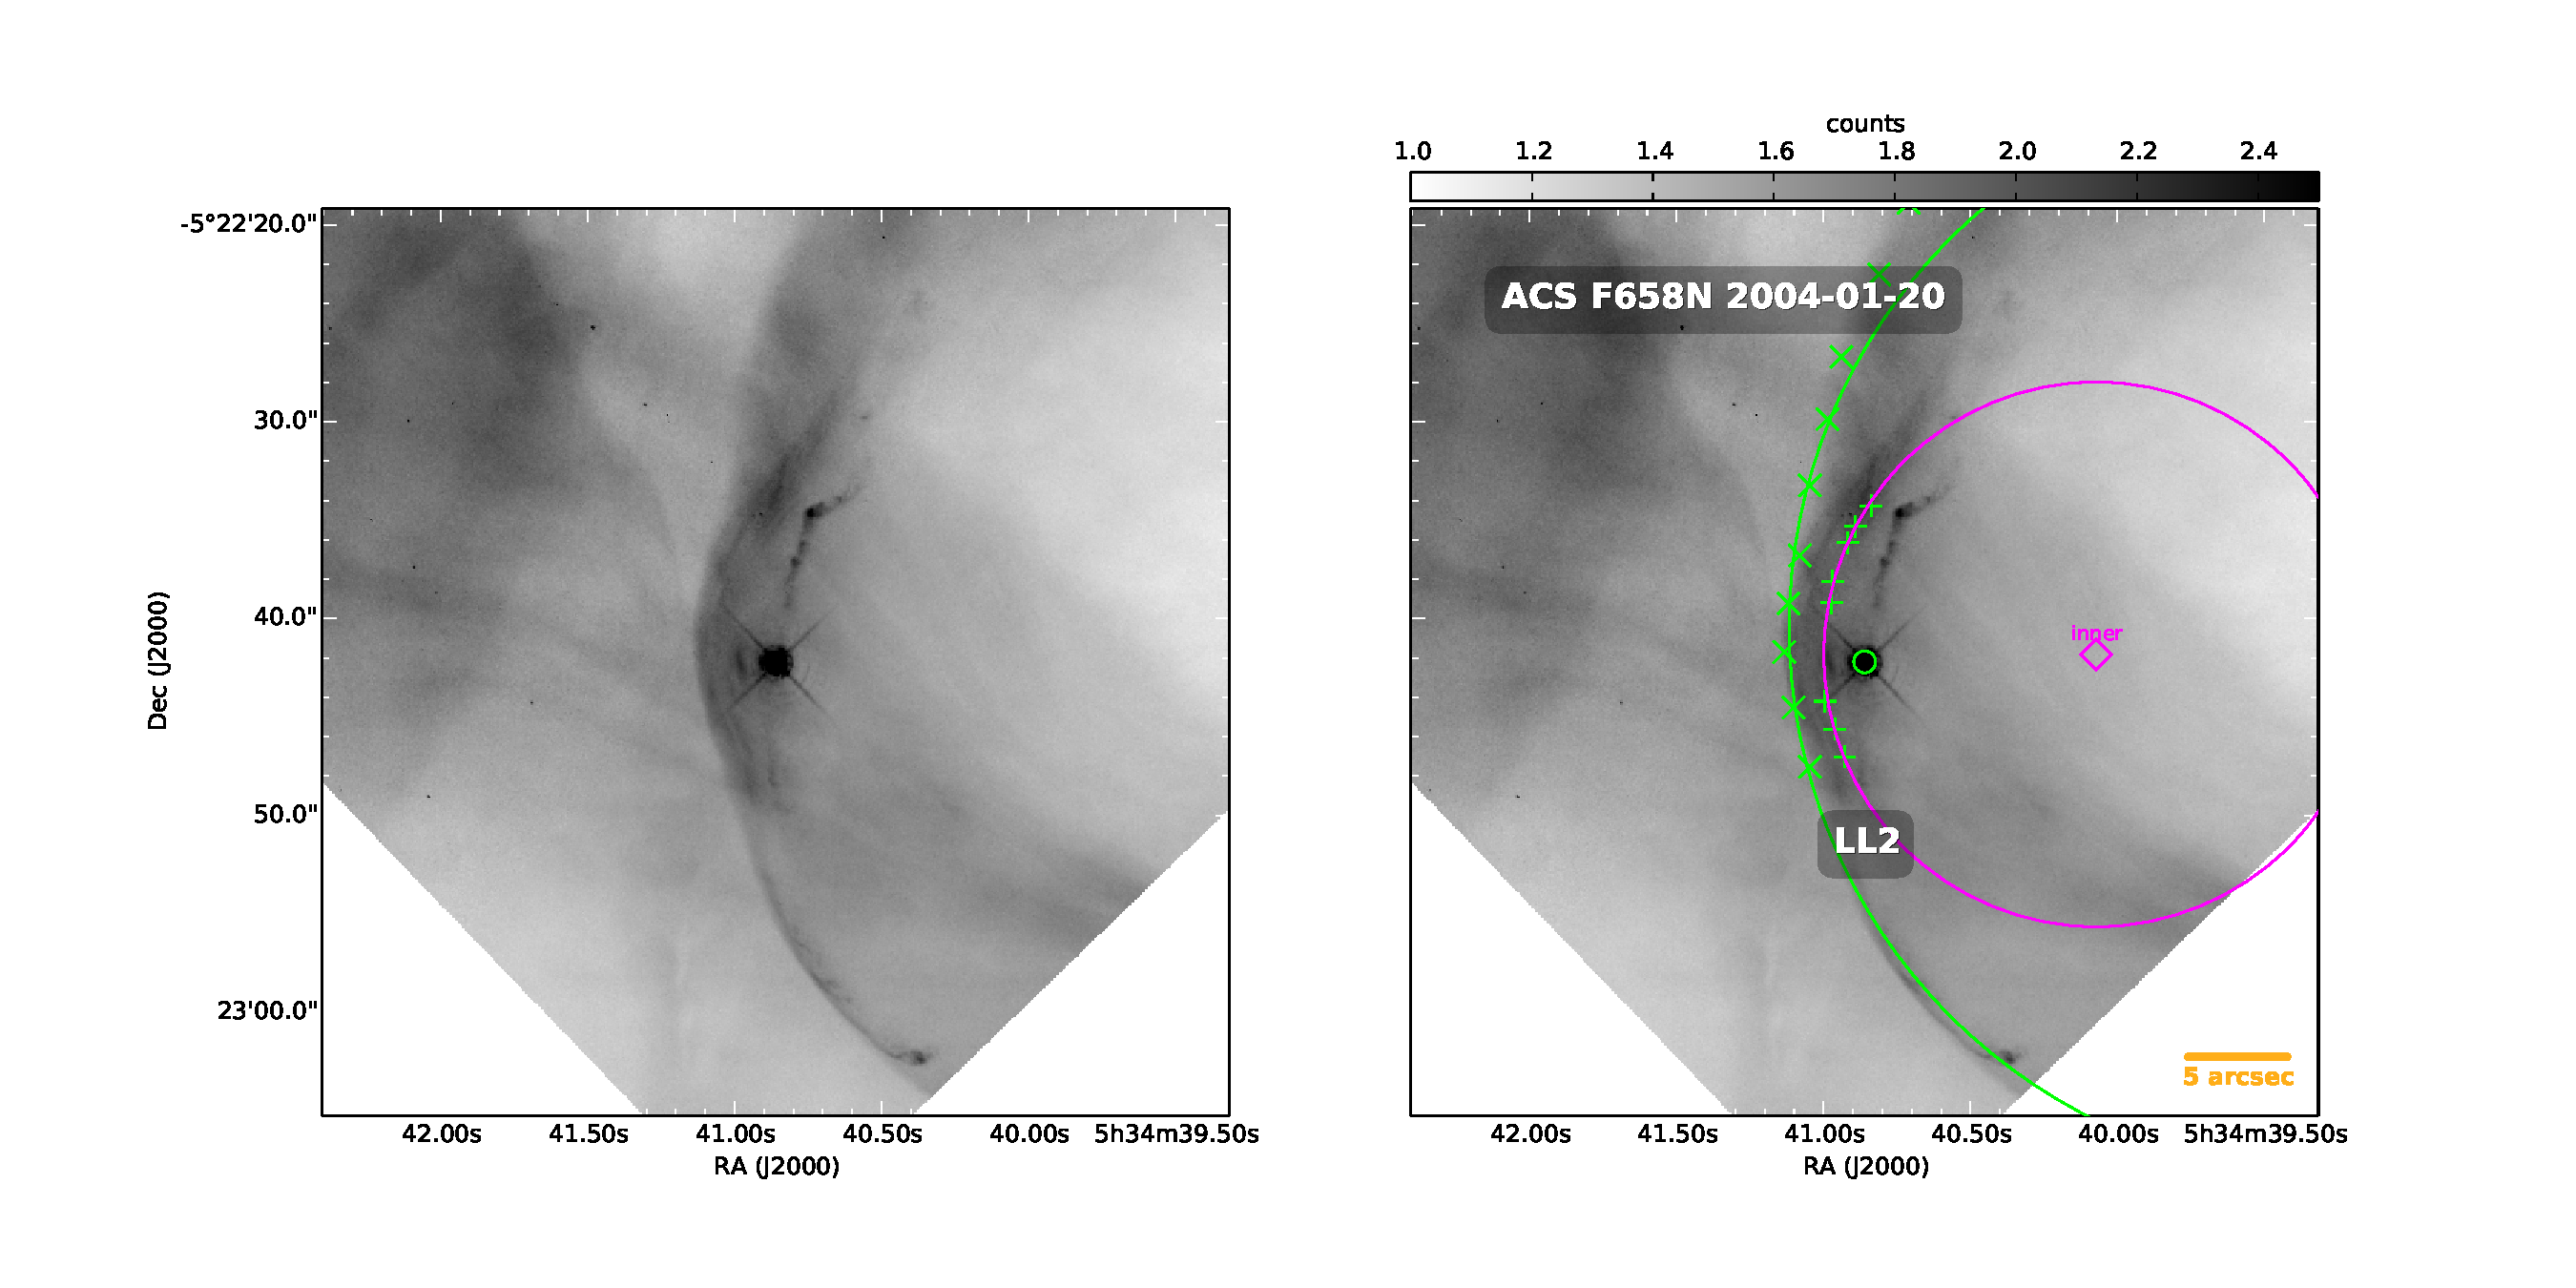
\includegraphics[width=\figwidth,  trim=60 50 100 50, clip]{j8oc18010_wcs/LL2-Bally_18-images.pdf}} 
   &\framebox{\includegraphics[width=\figwidth,  trim=60 50 100 50, clip]{j8oc17010_wcs/LL3-Bally_17-images.pdf}}\\ 
   \framebox{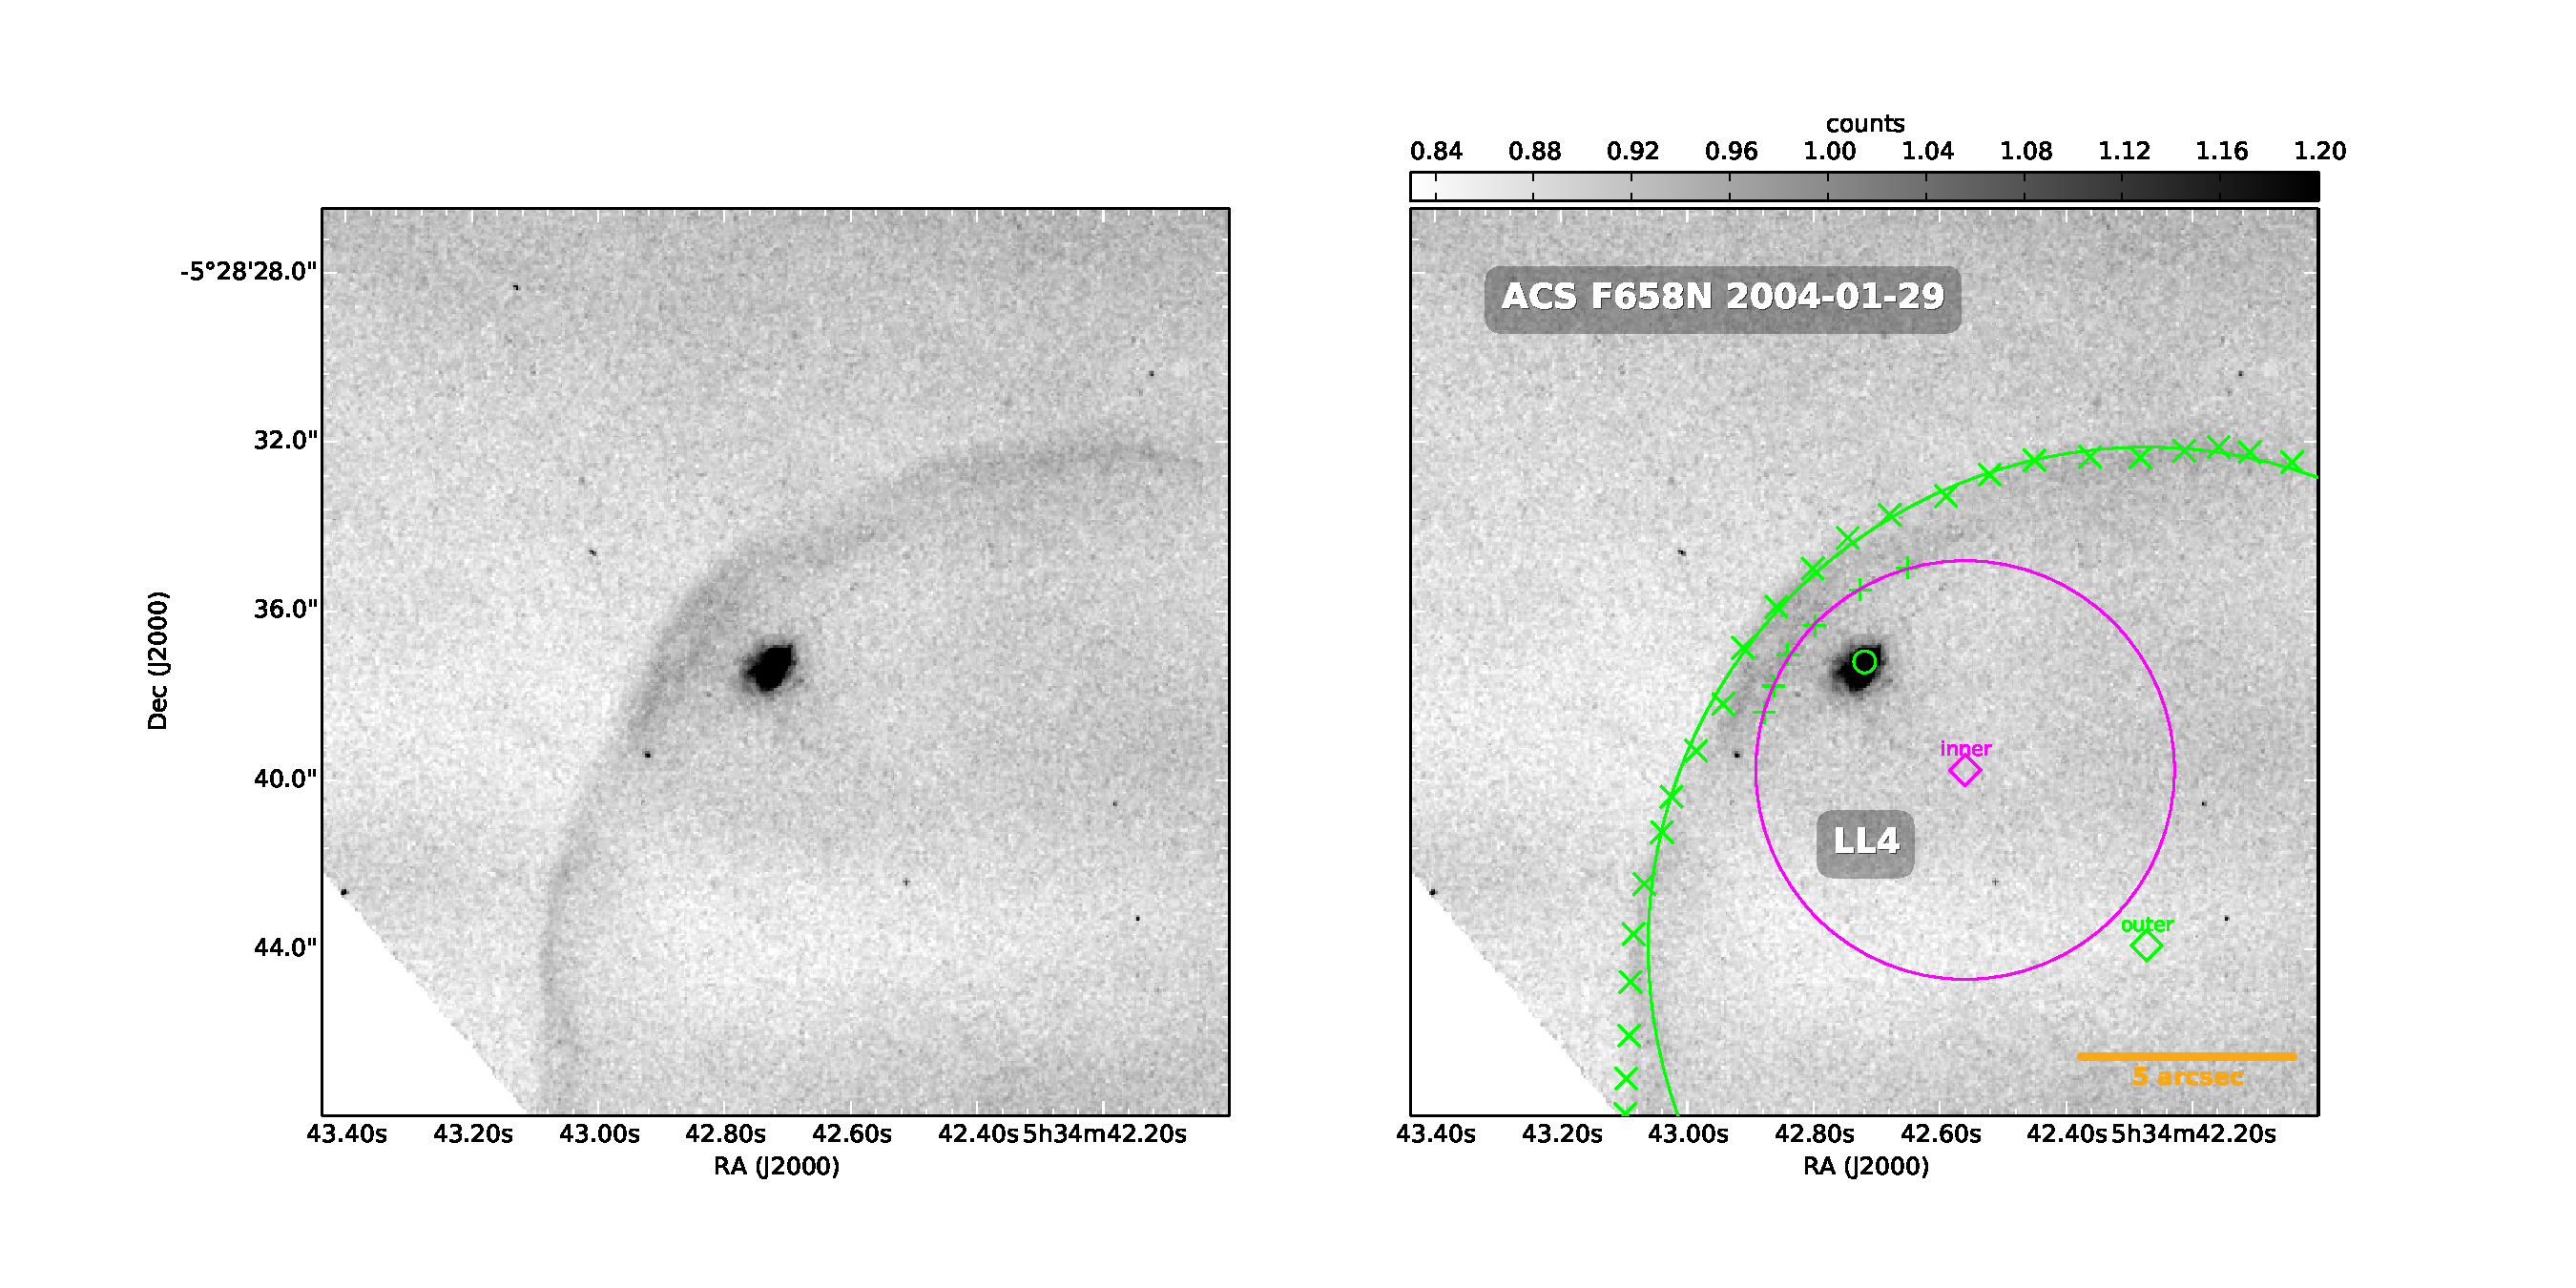
\includegraphics[width=\figwidth,  trim=60 50 100 50, clip]{j8oc24010_wcs/LL4-Bally_24-images.pdf}}
   &\framebox{\includegraphics[width=\figwidth,  trim=60 50 100 50, clip]{j8oc17010_wcs/4468-605-Bally_17-images.pdf}}\\
   \framebox{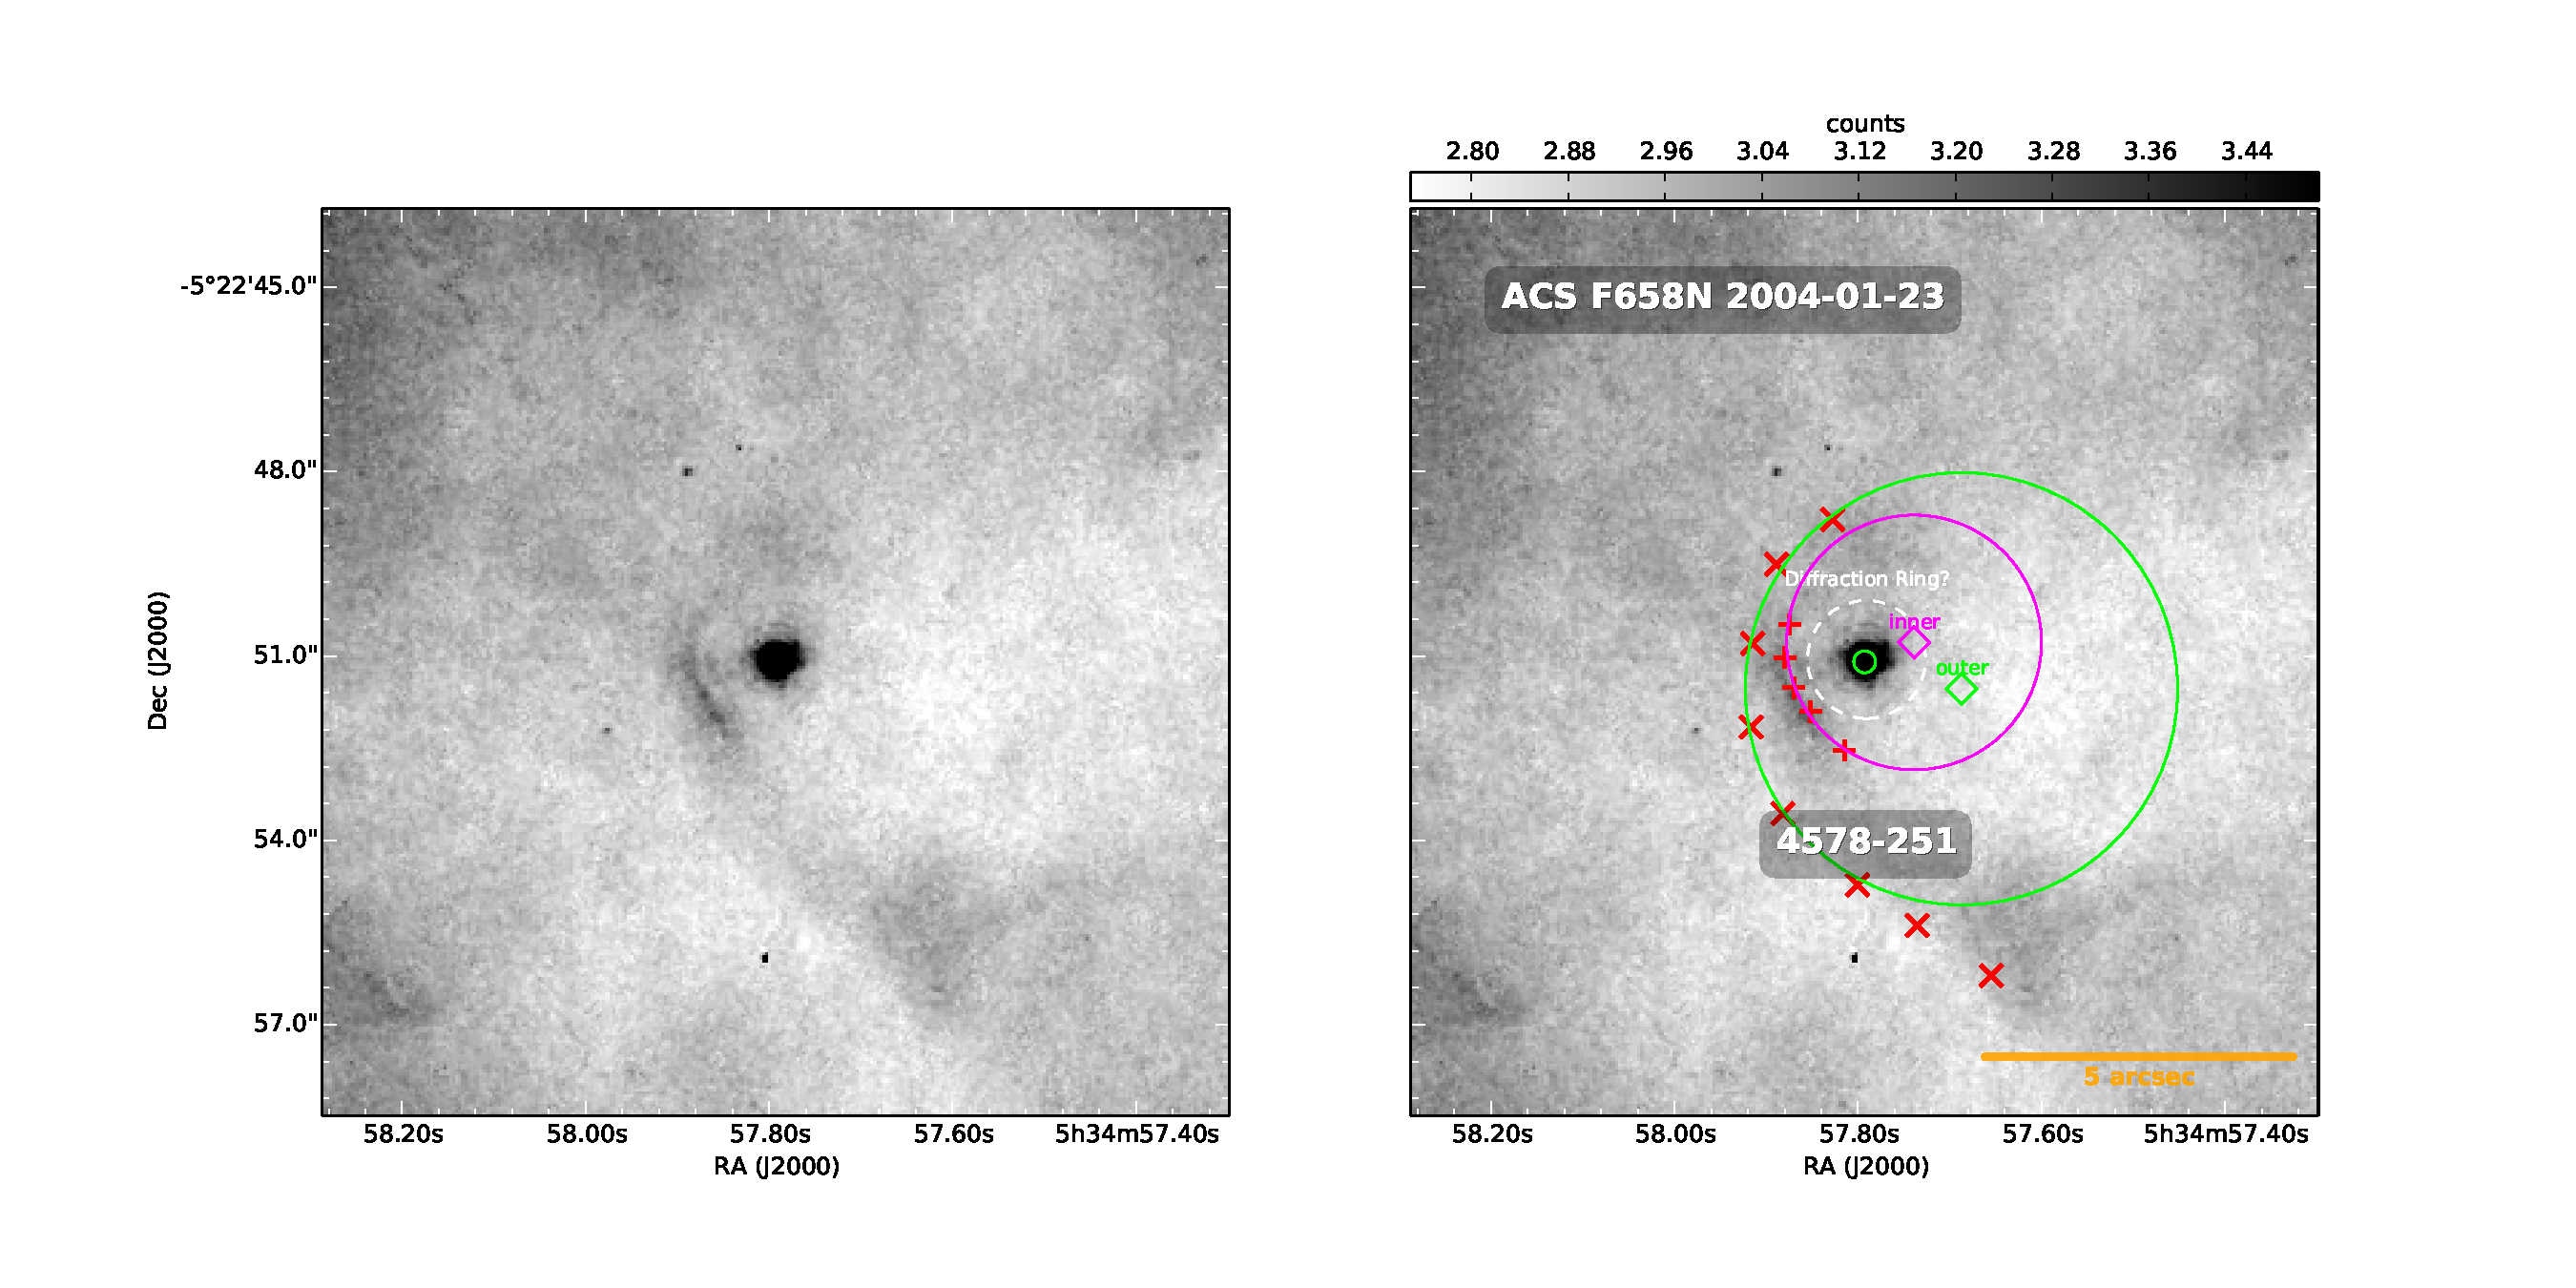
\includegraphics[width=\figwidth,  trim=60 50 100 50, clip]{j8oc09010_wcs/4578-251-Bally_09-images.pdf}}
   &\framebox{\includegraphics[width=\figwidth,  trim=60 50 100 50, clip]{j8oc16010_wcs/4582-635-Bally_16-images.pdf}}\\ 
    \framebox{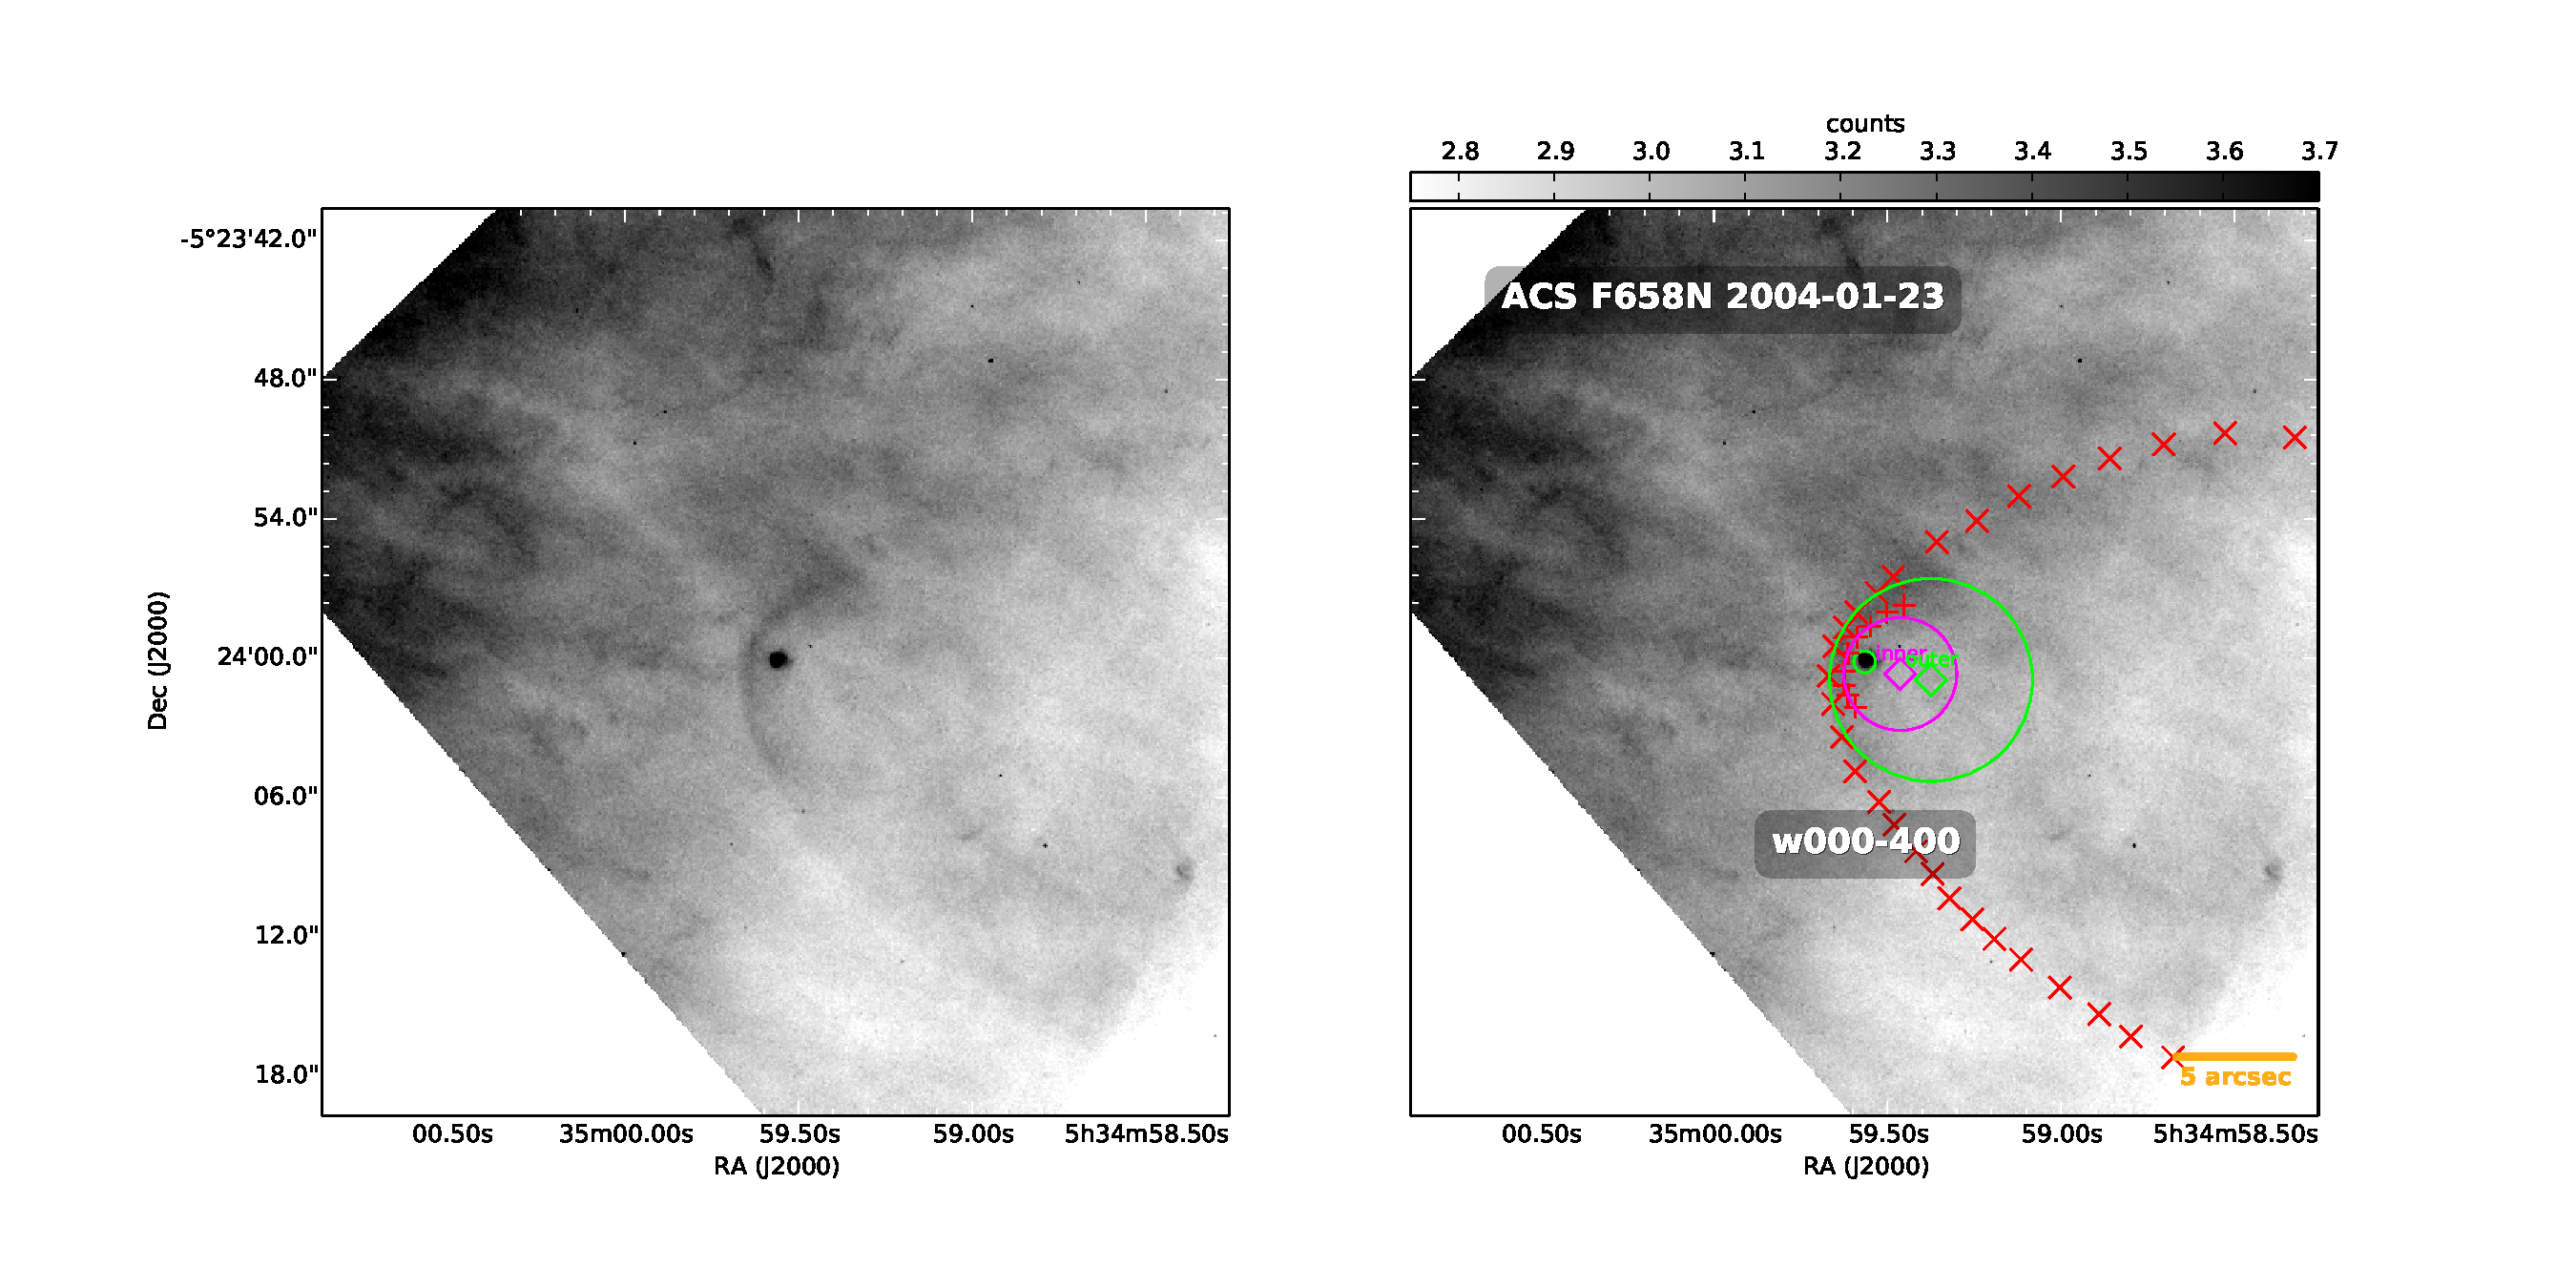
\includegraphics[width=\figwidth, trim=60 50 100 50, clip]{j8oc09010_wcs/w000-400-Bally_09-images.pdf}}
   &\framebox{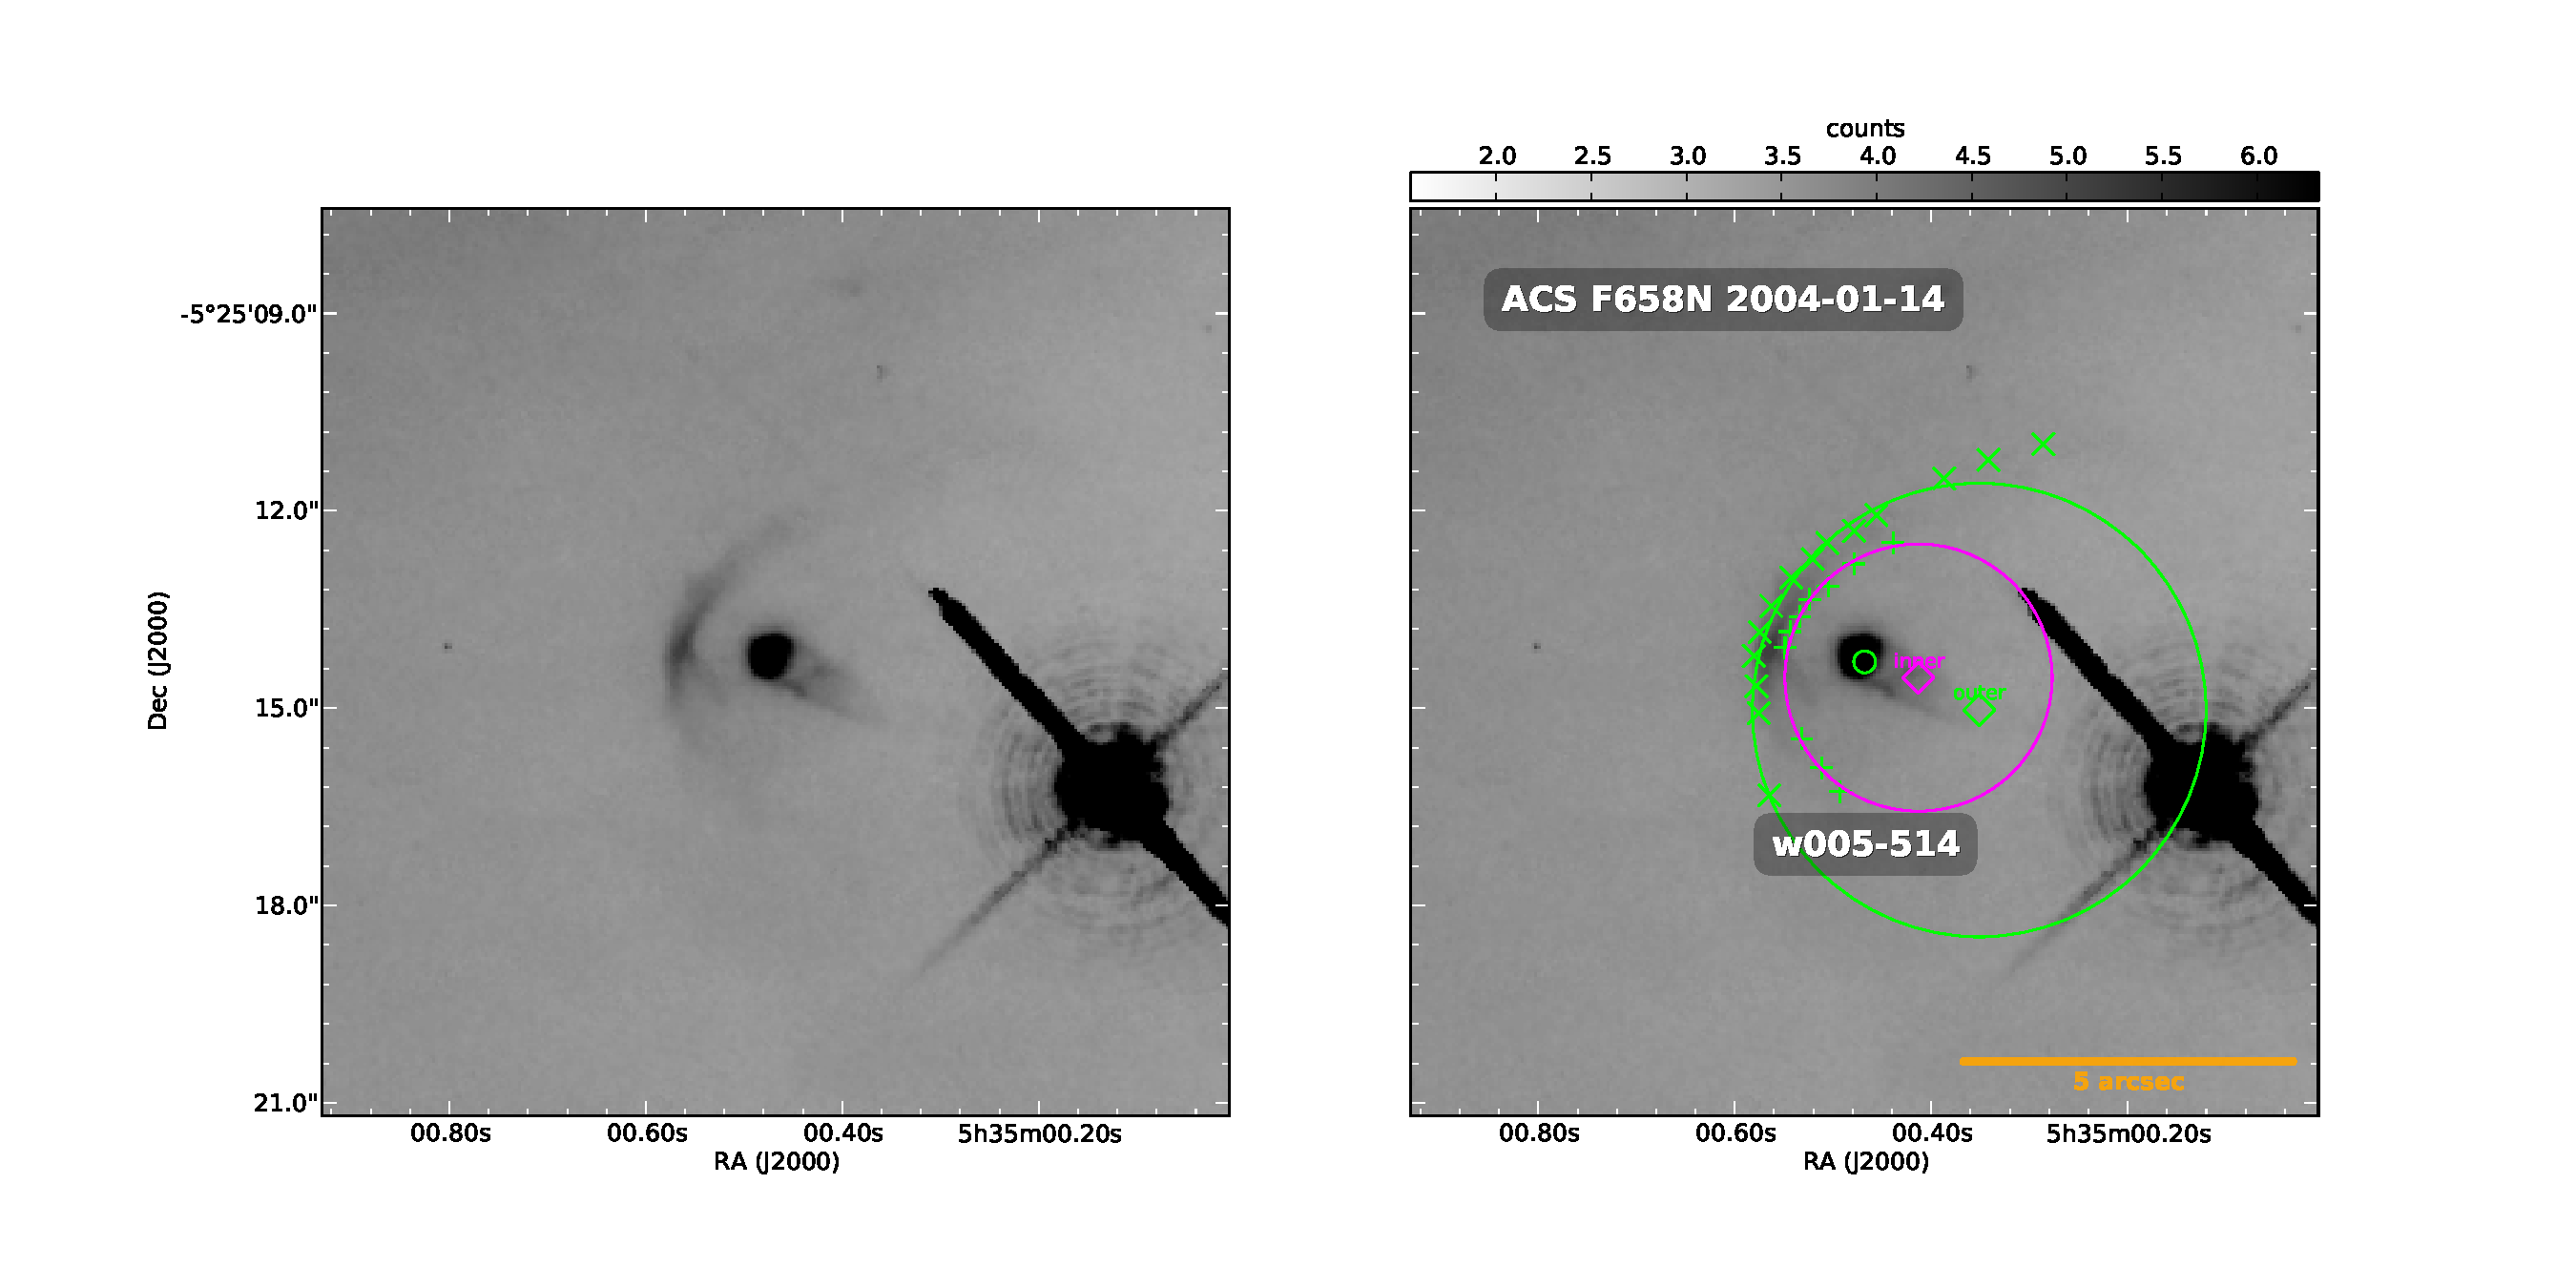
\includegraphics[width=\figwidth, trim=60 50 100 50, clip]{j8oc01010_wcs/w005-514-Bally_01-images.pdf}}\\  
   \framebox{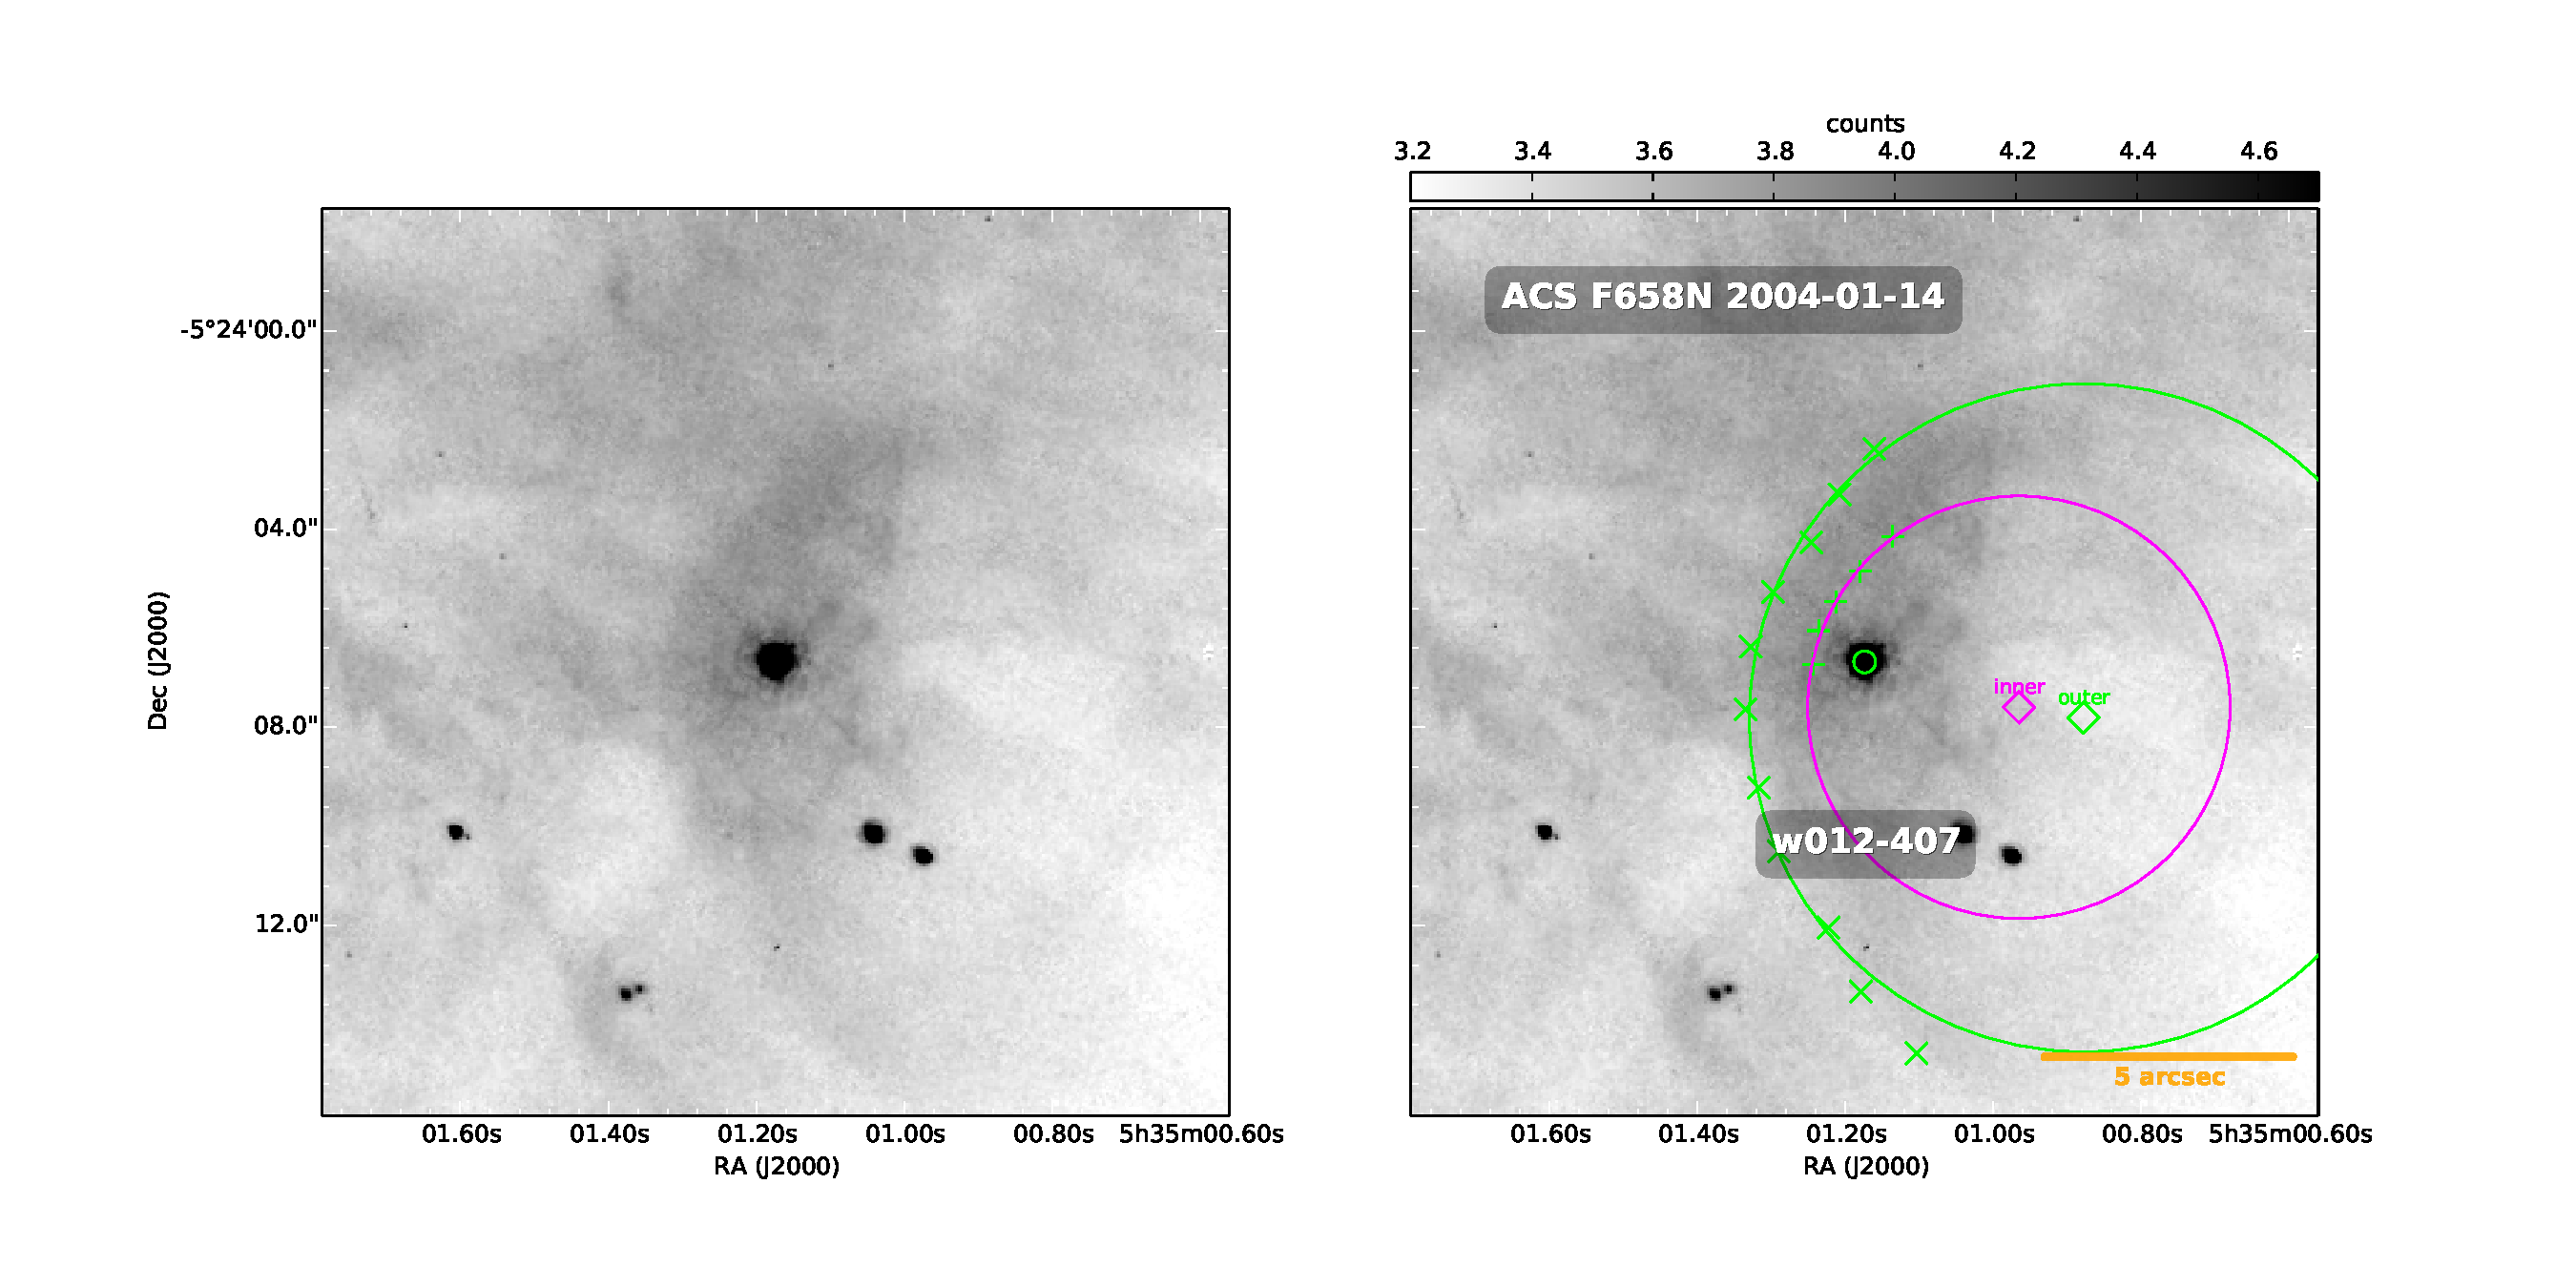
\includegraphics[width=\figwidth, trim=60 50 100 50, clip]{j8oc01010_wcs/w012-407-Bally_01-images.pdf}}
   &\framebox{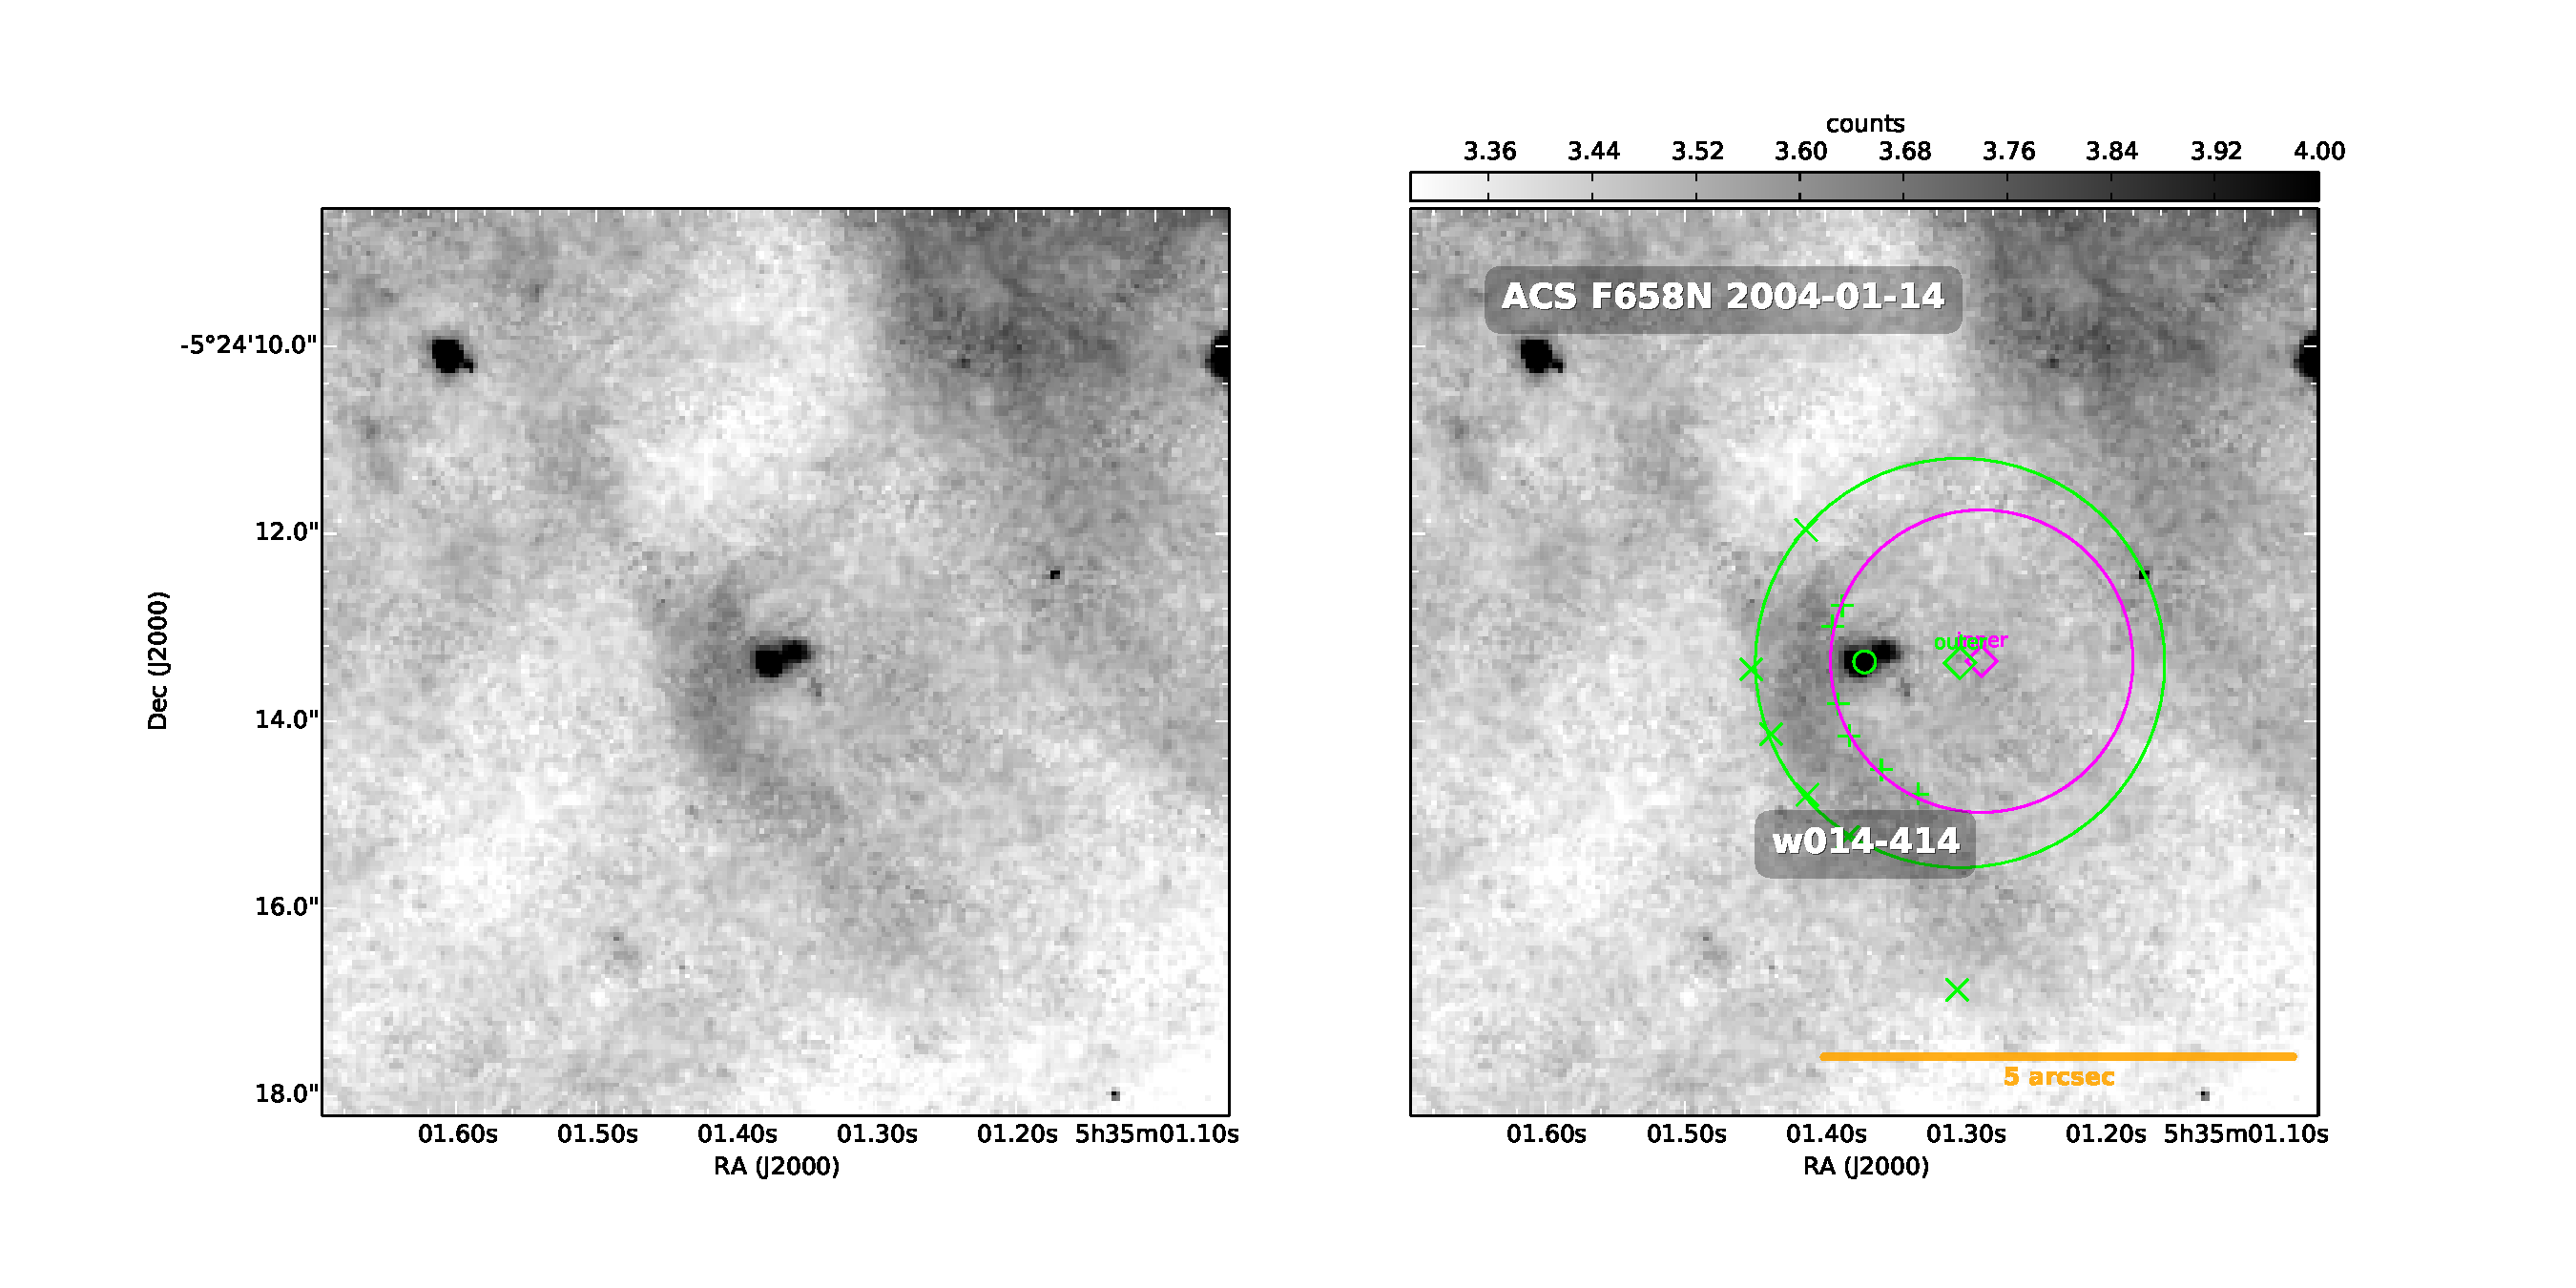
\includegraphics[width=\figwidth, trim=60 50 100 50, clip]{j8oc01010_wcs/w014-414-Bally_01-images.pdf}}\\ 
   \framebox{\includegraphics[width=\figwidth, trim=60 50 100 50, clip]{j8oc16010_wcs/022-635-Bally_16-images.pdf}}
   &\framebox{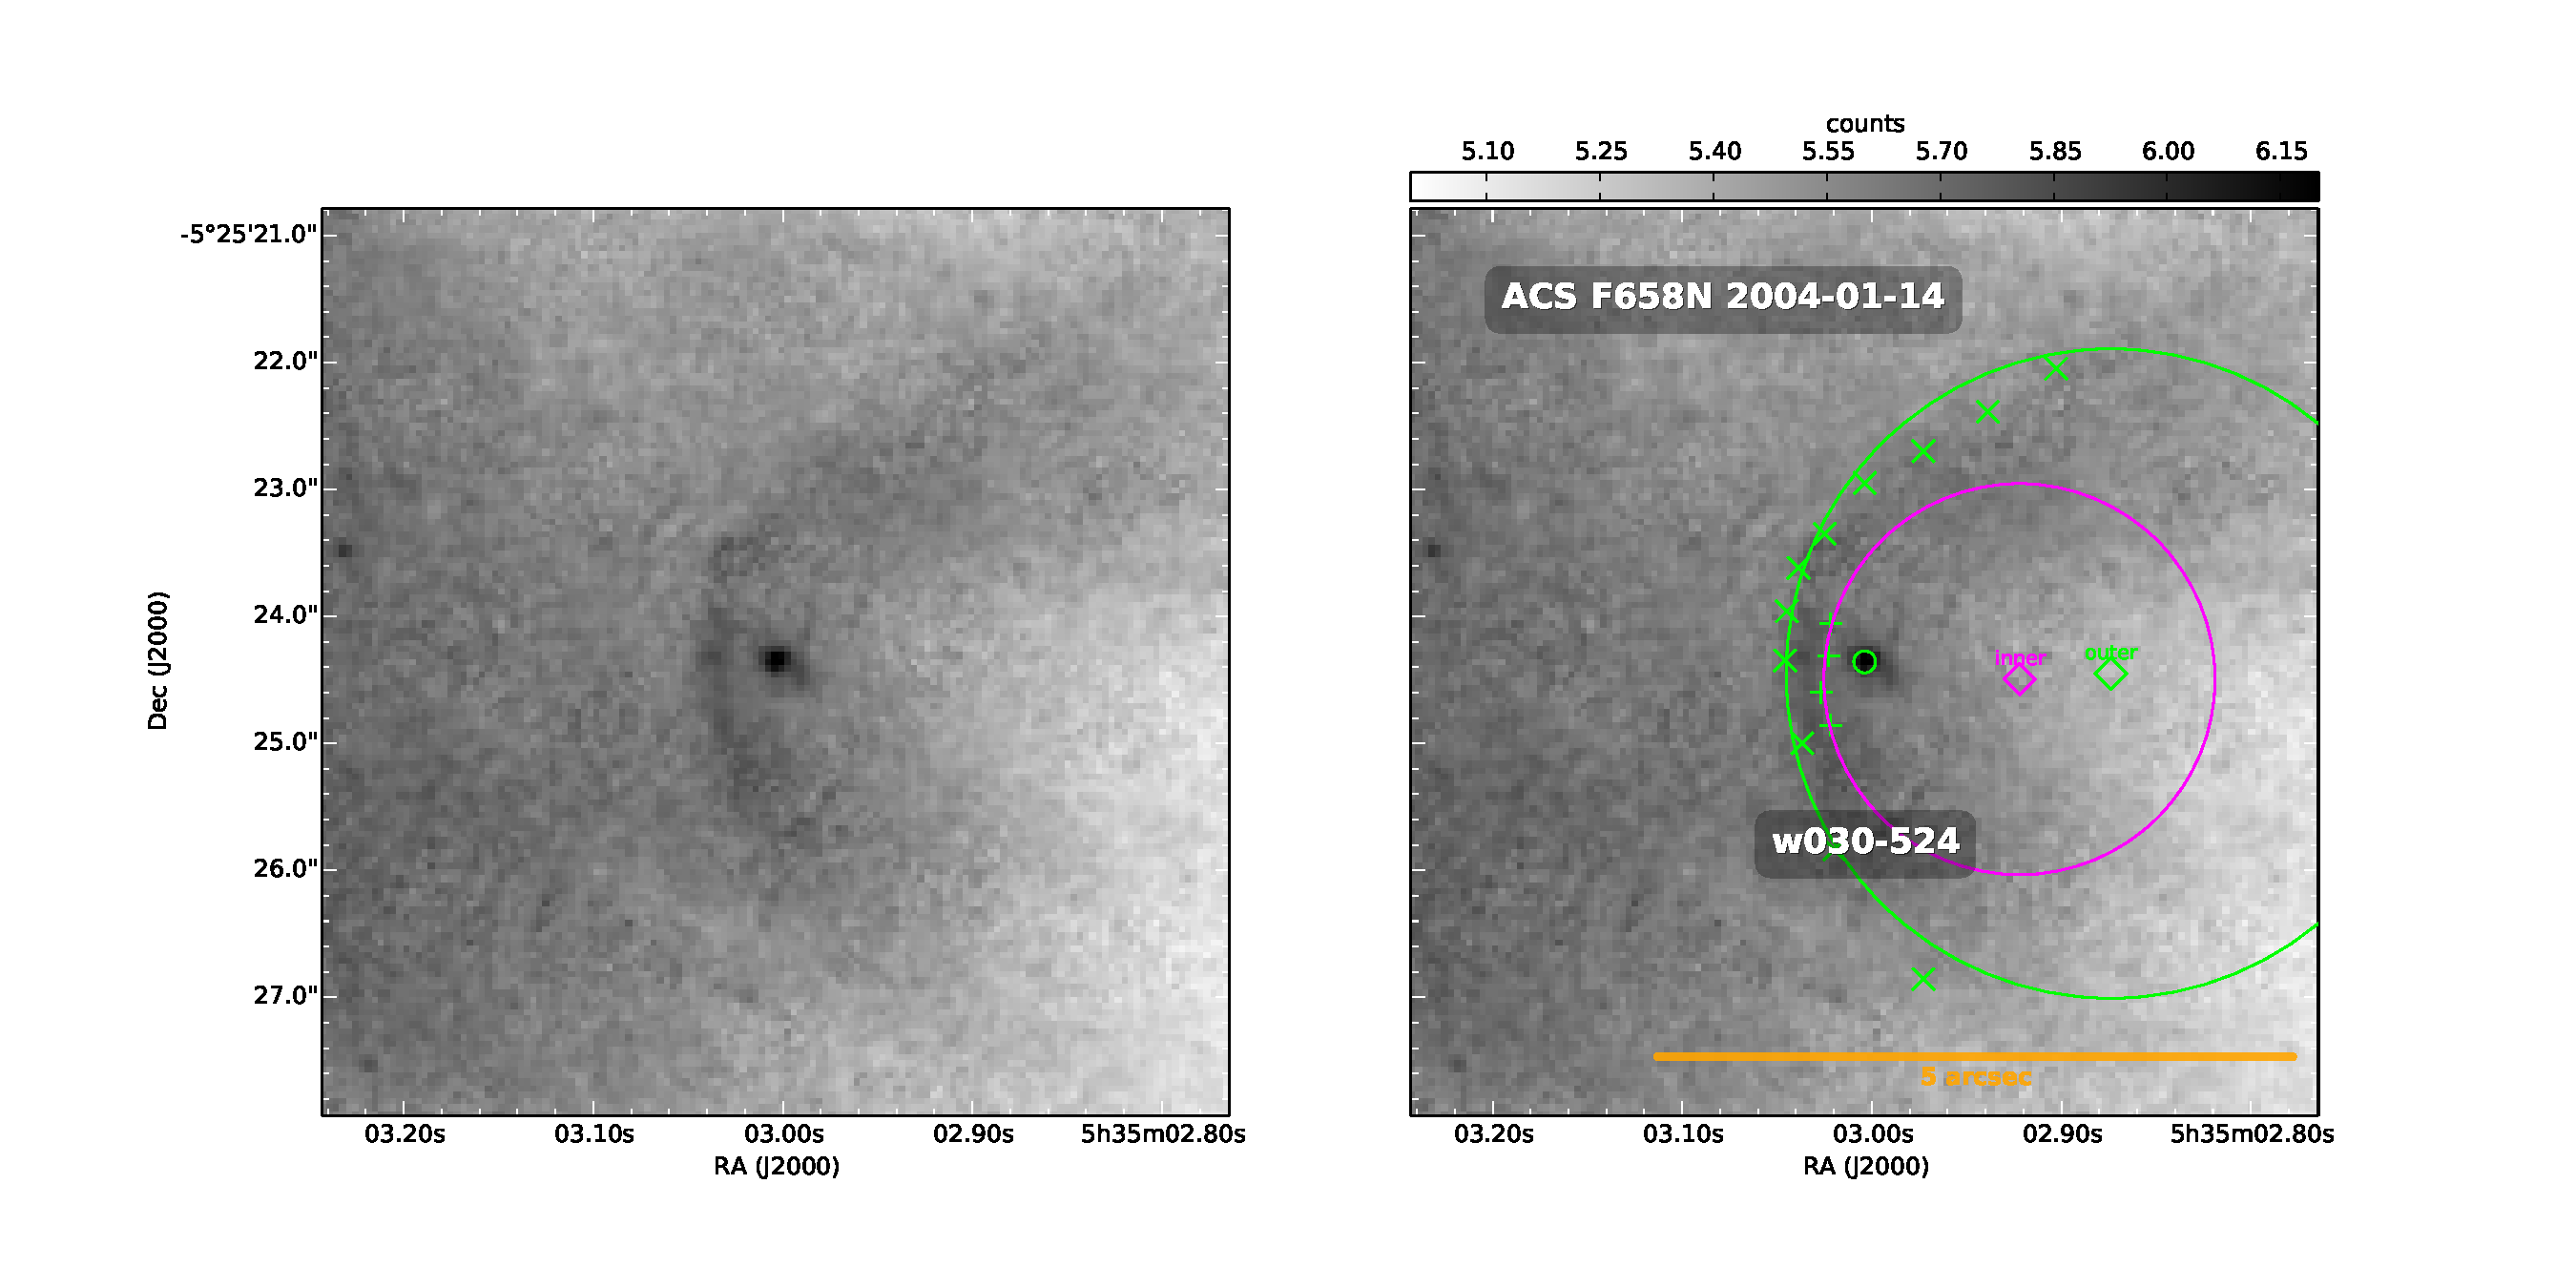
\includegraphics[width=\figwidth, trim=60 50 100 50, clip]{j8oc01010_wcs/w030-524-Bally_01-images.pdf}}\\ 
\end{tabular}
\end{figure*}

\begin{figure*}
\setlength\tabcolsep{1.5pt}
\begin{tabular}{l l}

   \framebox{\includegraphics[width=\figwidth,  trim=60 50 100 50, clip]{j8oc16010_wcs/041-637-Bally_16-images.pdf}}
   &\framebox{\includegraphics[width=\figwidth,  trim=60 50 100 50, clip]{j8oc16010_wcs/042-628-Bally_16-images.pdf}}\\ 
   \framebox{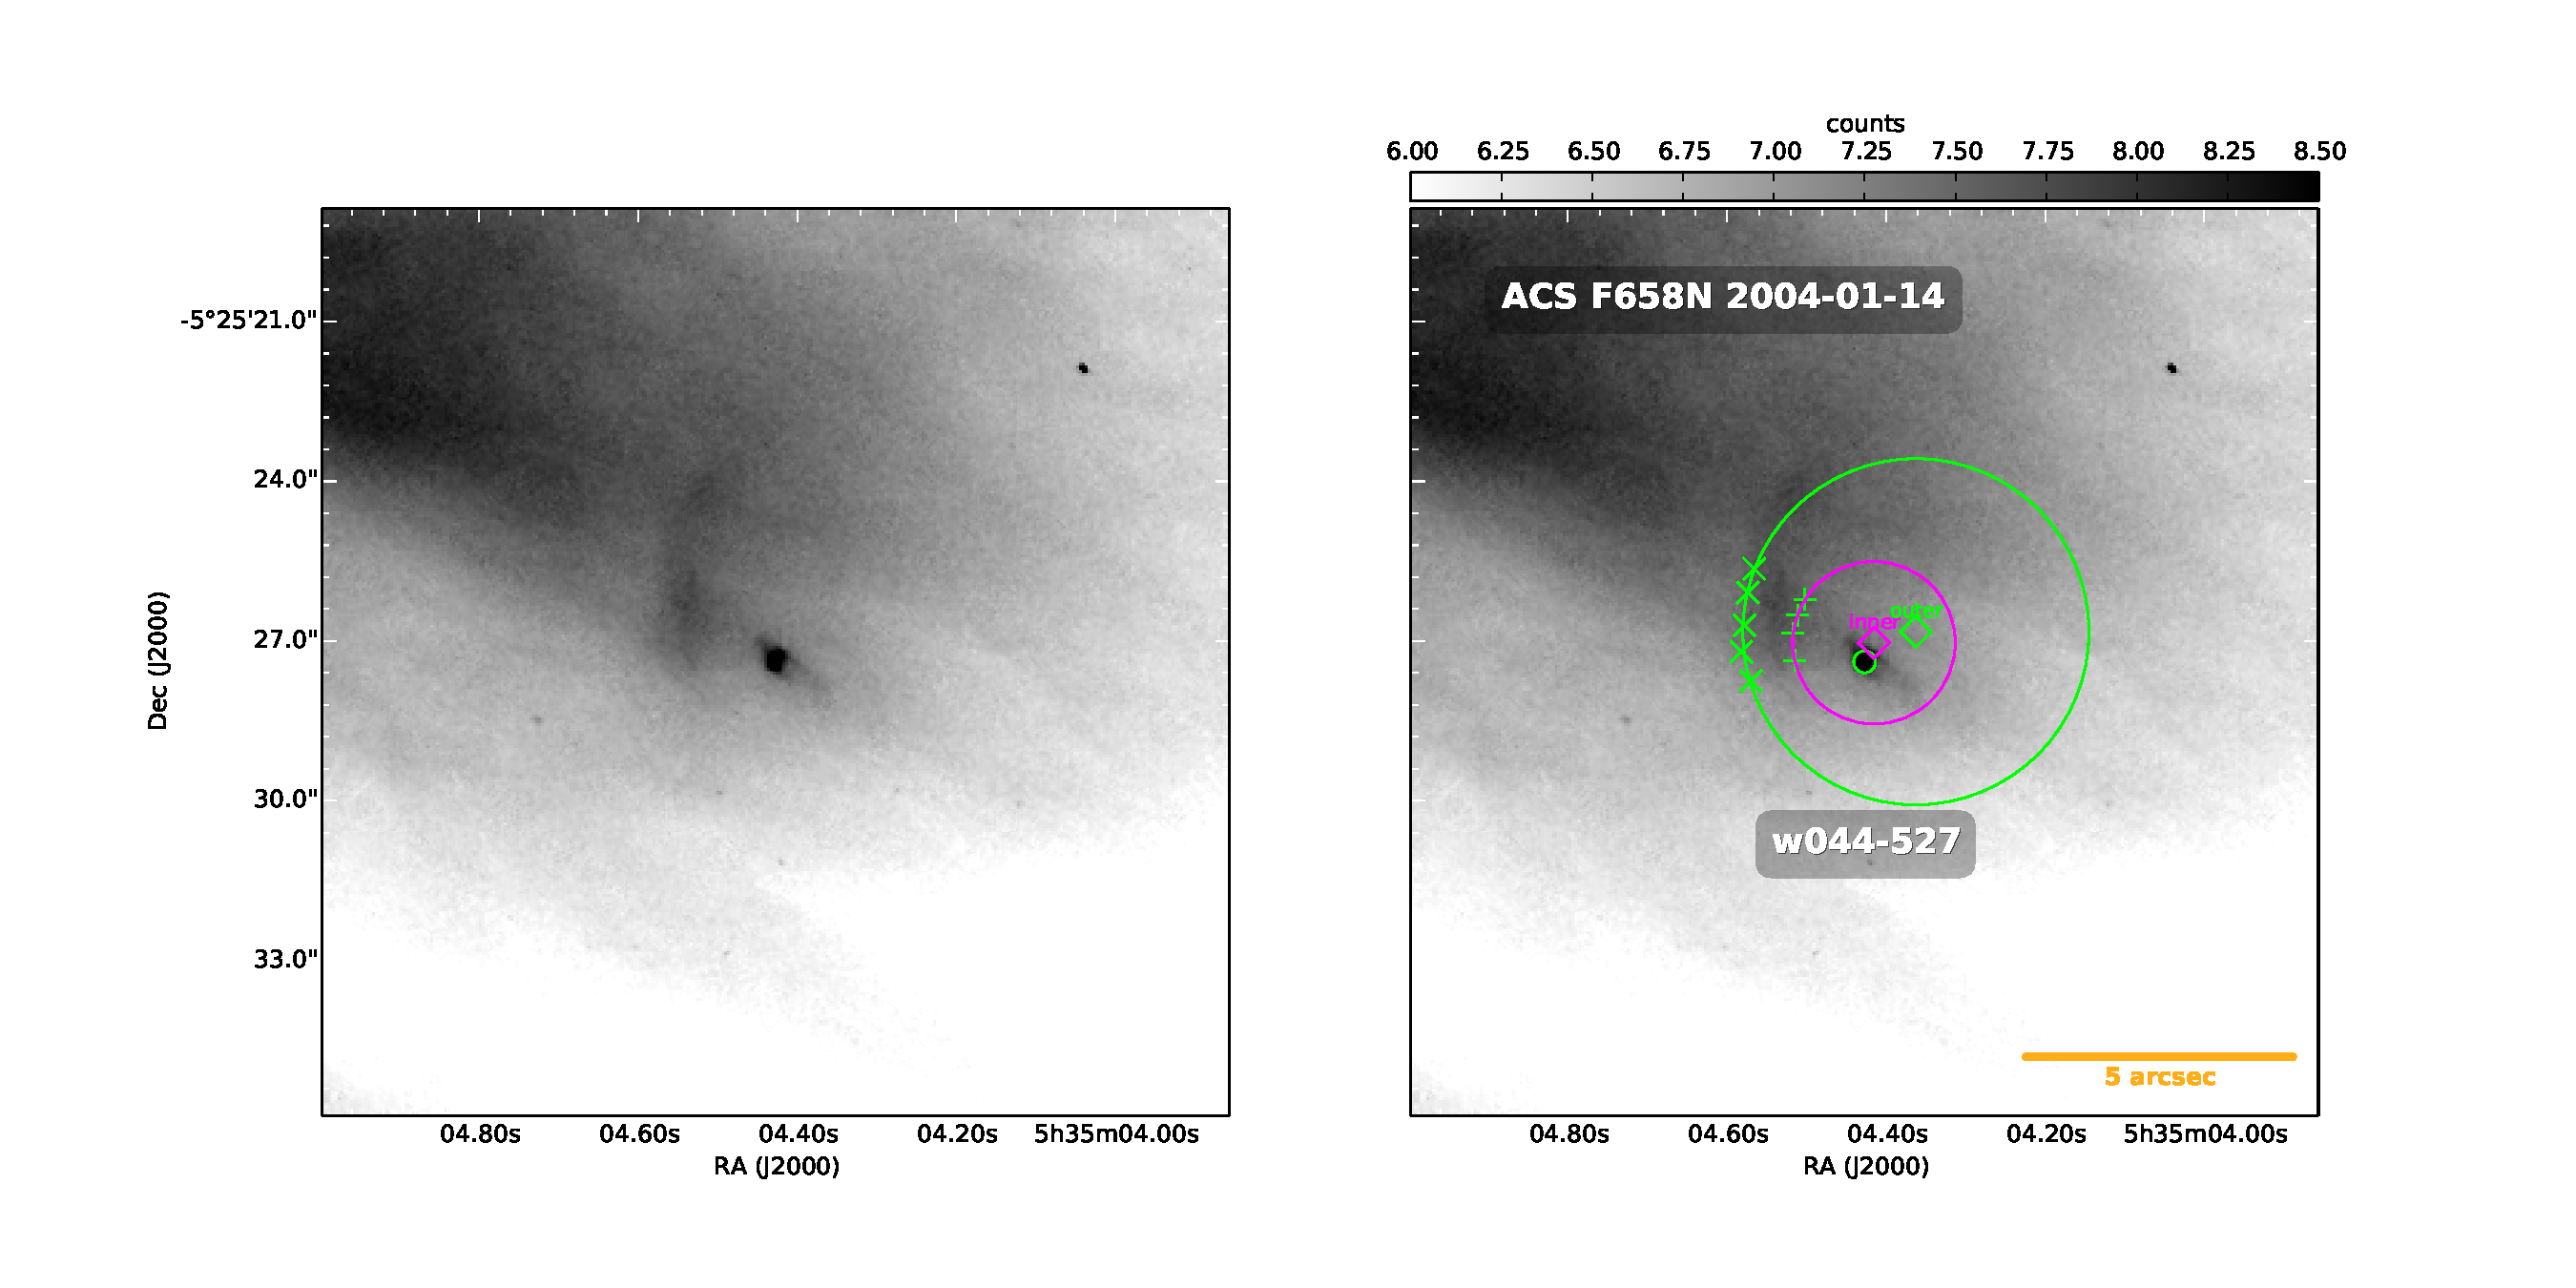
\includegraphics[width=\figwidth,  trim=60 50 100 50, clip]{j8oc01010_wcs/w044-527-Bally_01-images.pdf}}
   &\framebox{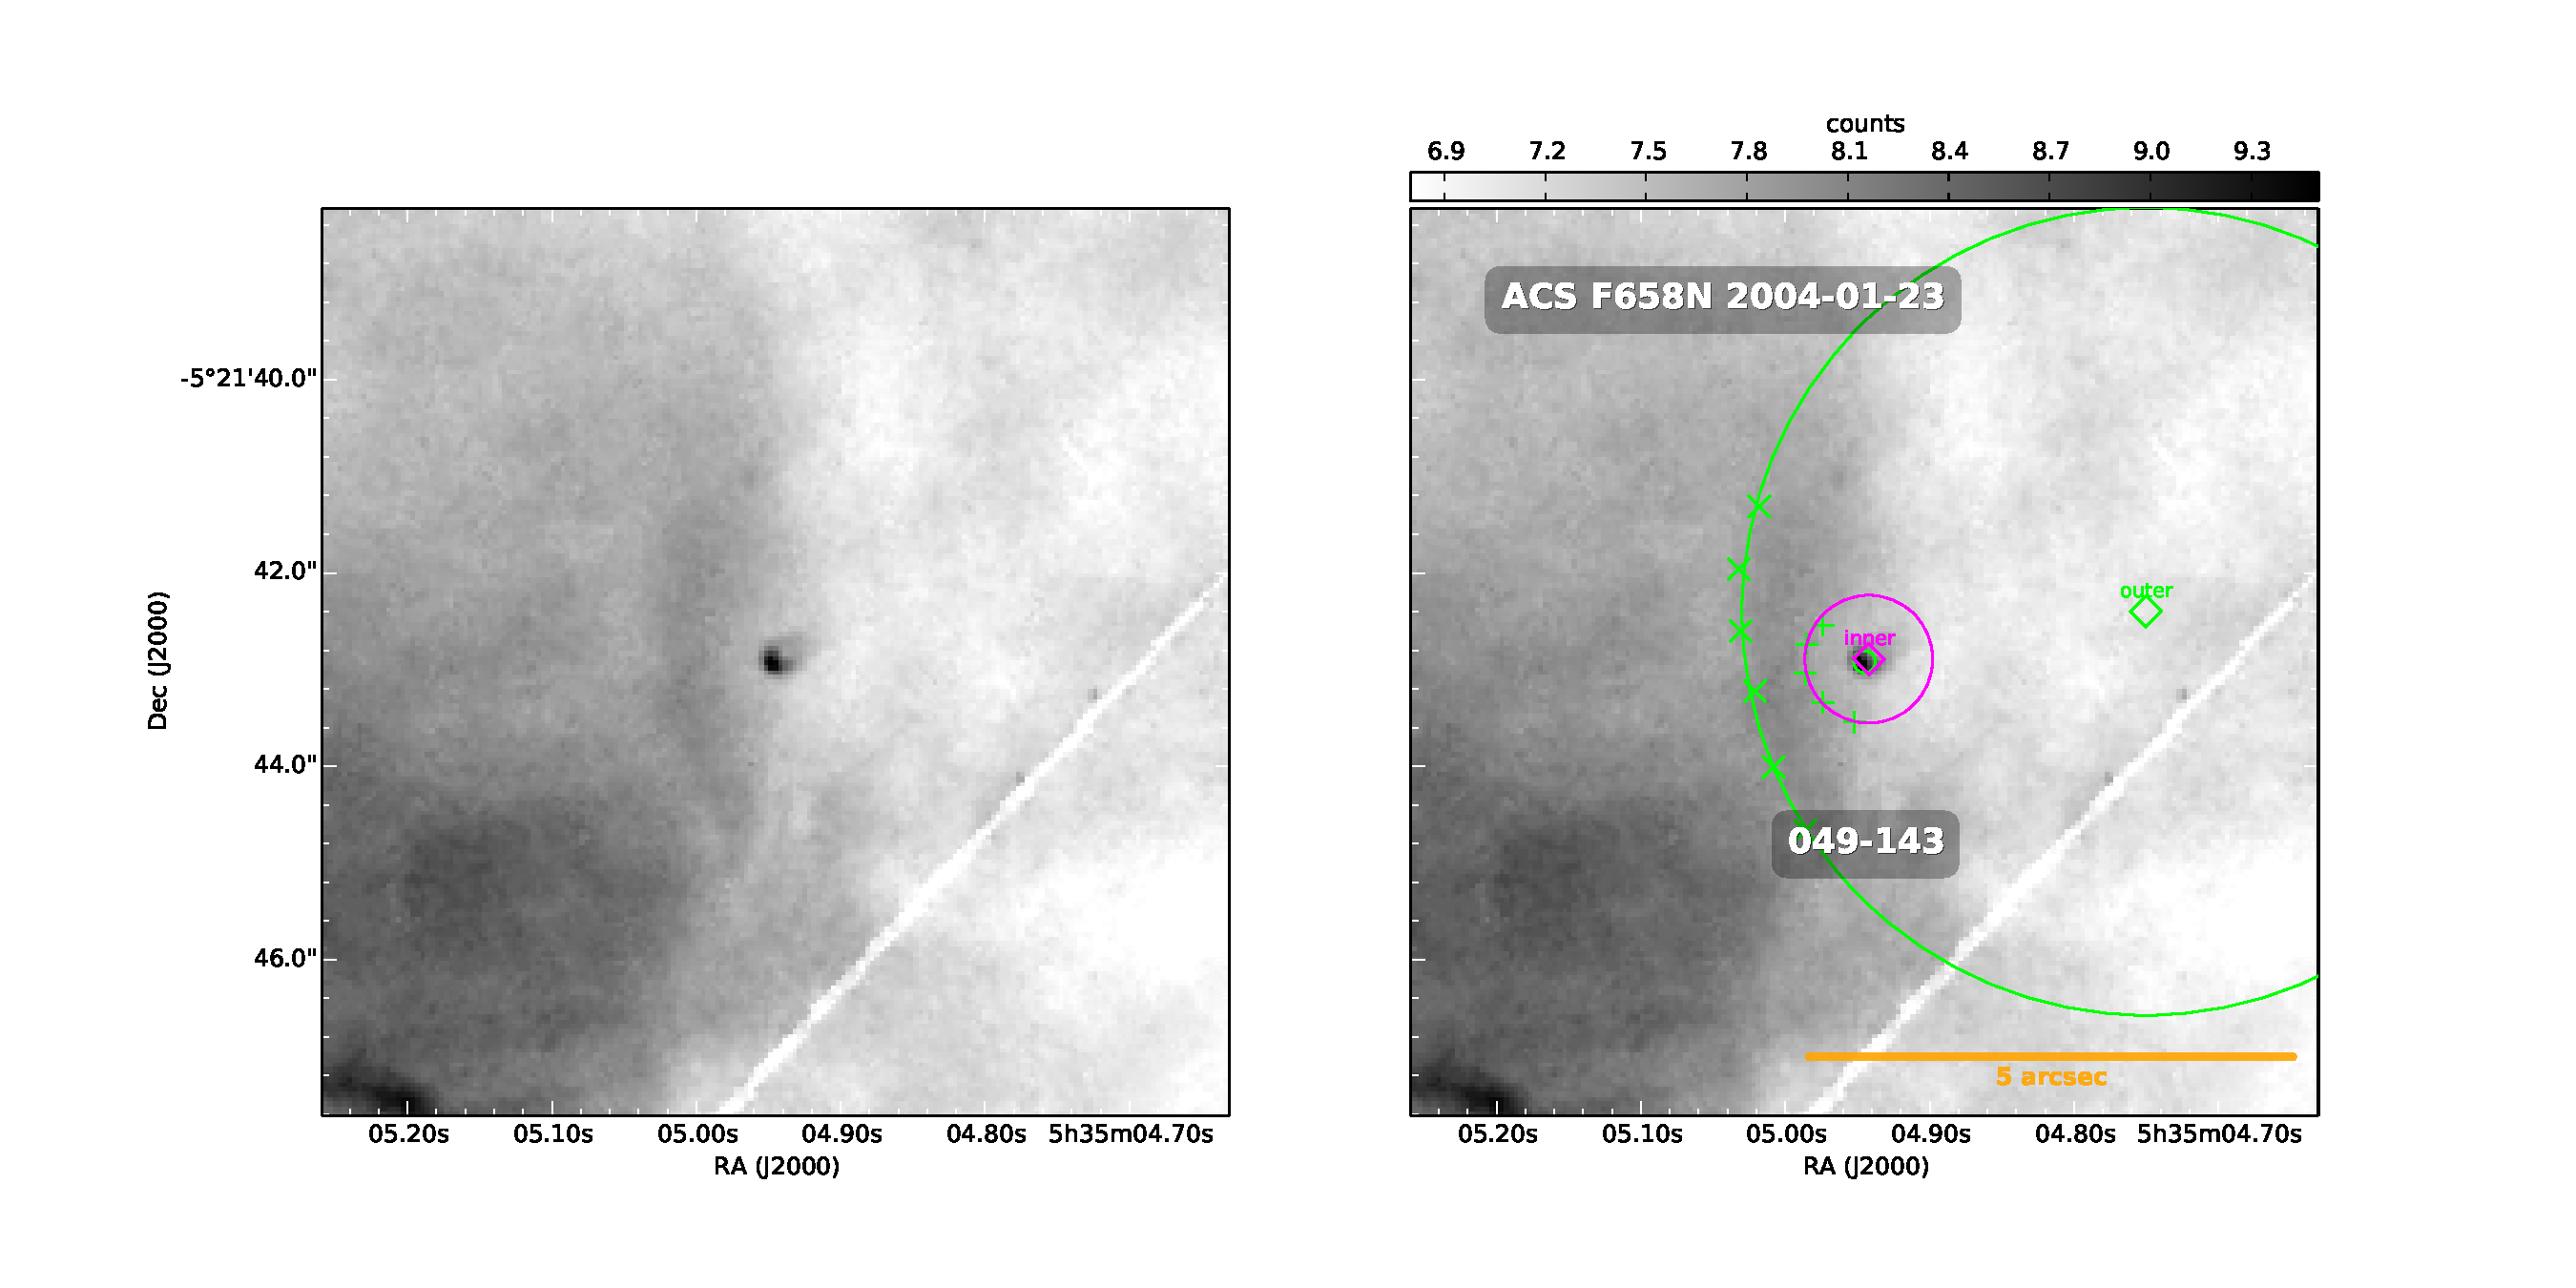
\includegraphics[width=\figwidth,  trim=60 50 100 50, clip]{j8oc09010_wcs/049-143-Bally_09-images.pdf}}\\ 
   \framebox{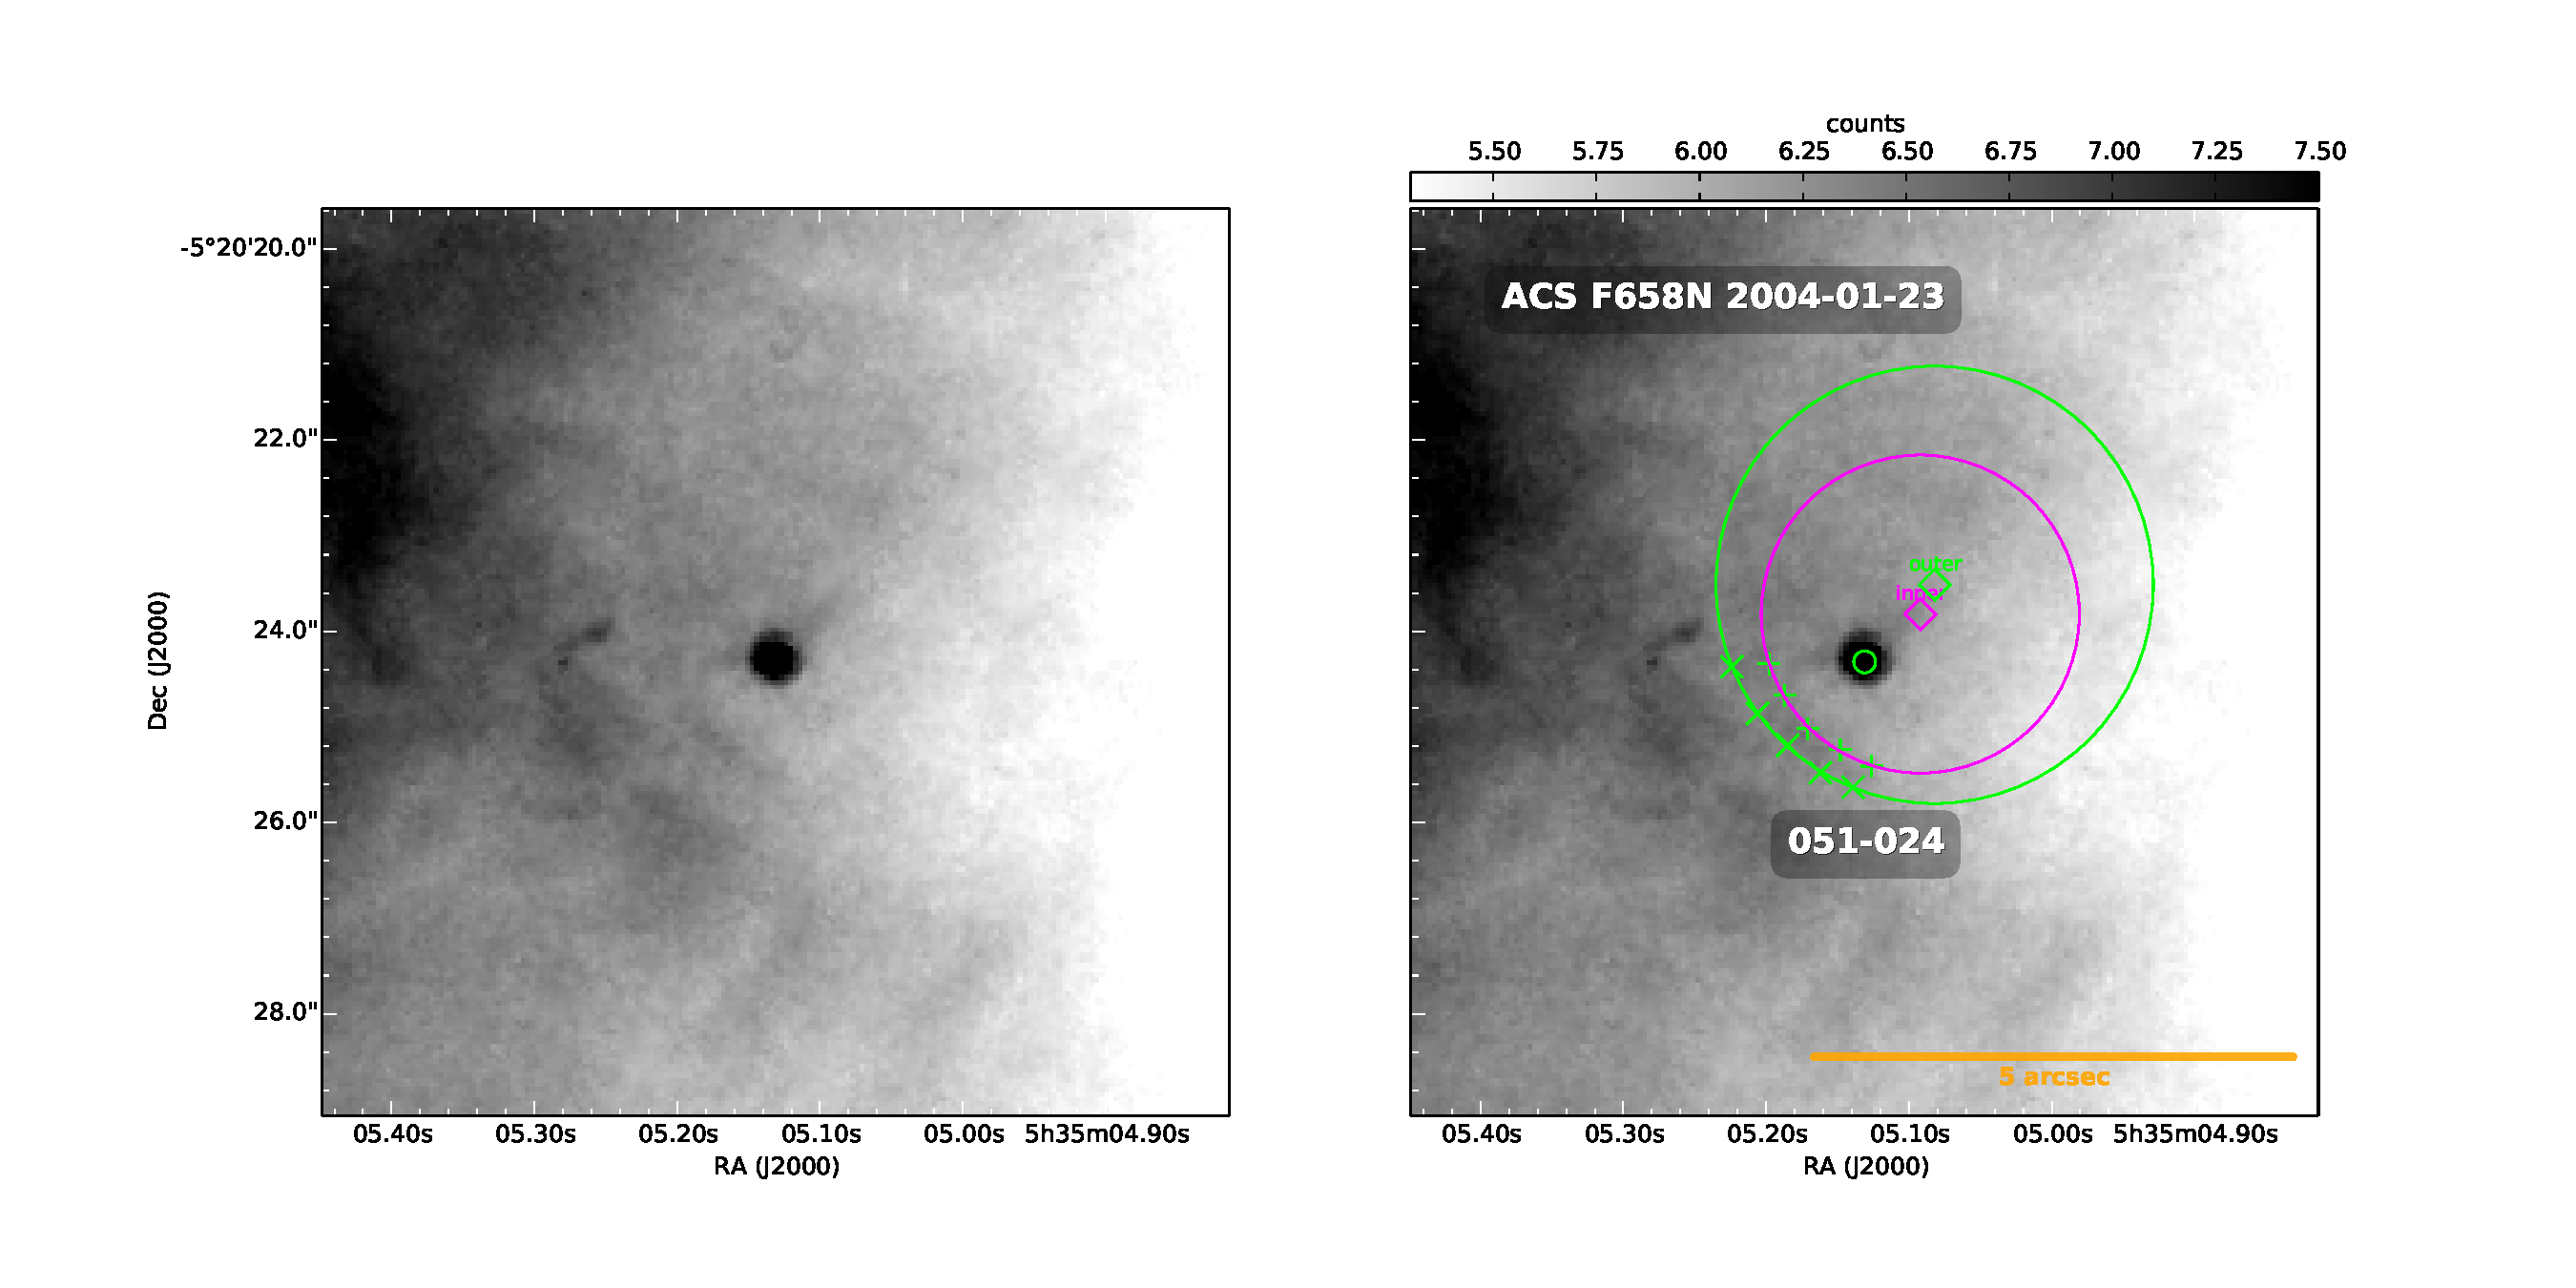
\includegraphics[width=\figwidth,  trim=60 50 100 50, clip]{j8oc09010_wcs/051-024-Bally_09-images.pdf}}
   &\framebox{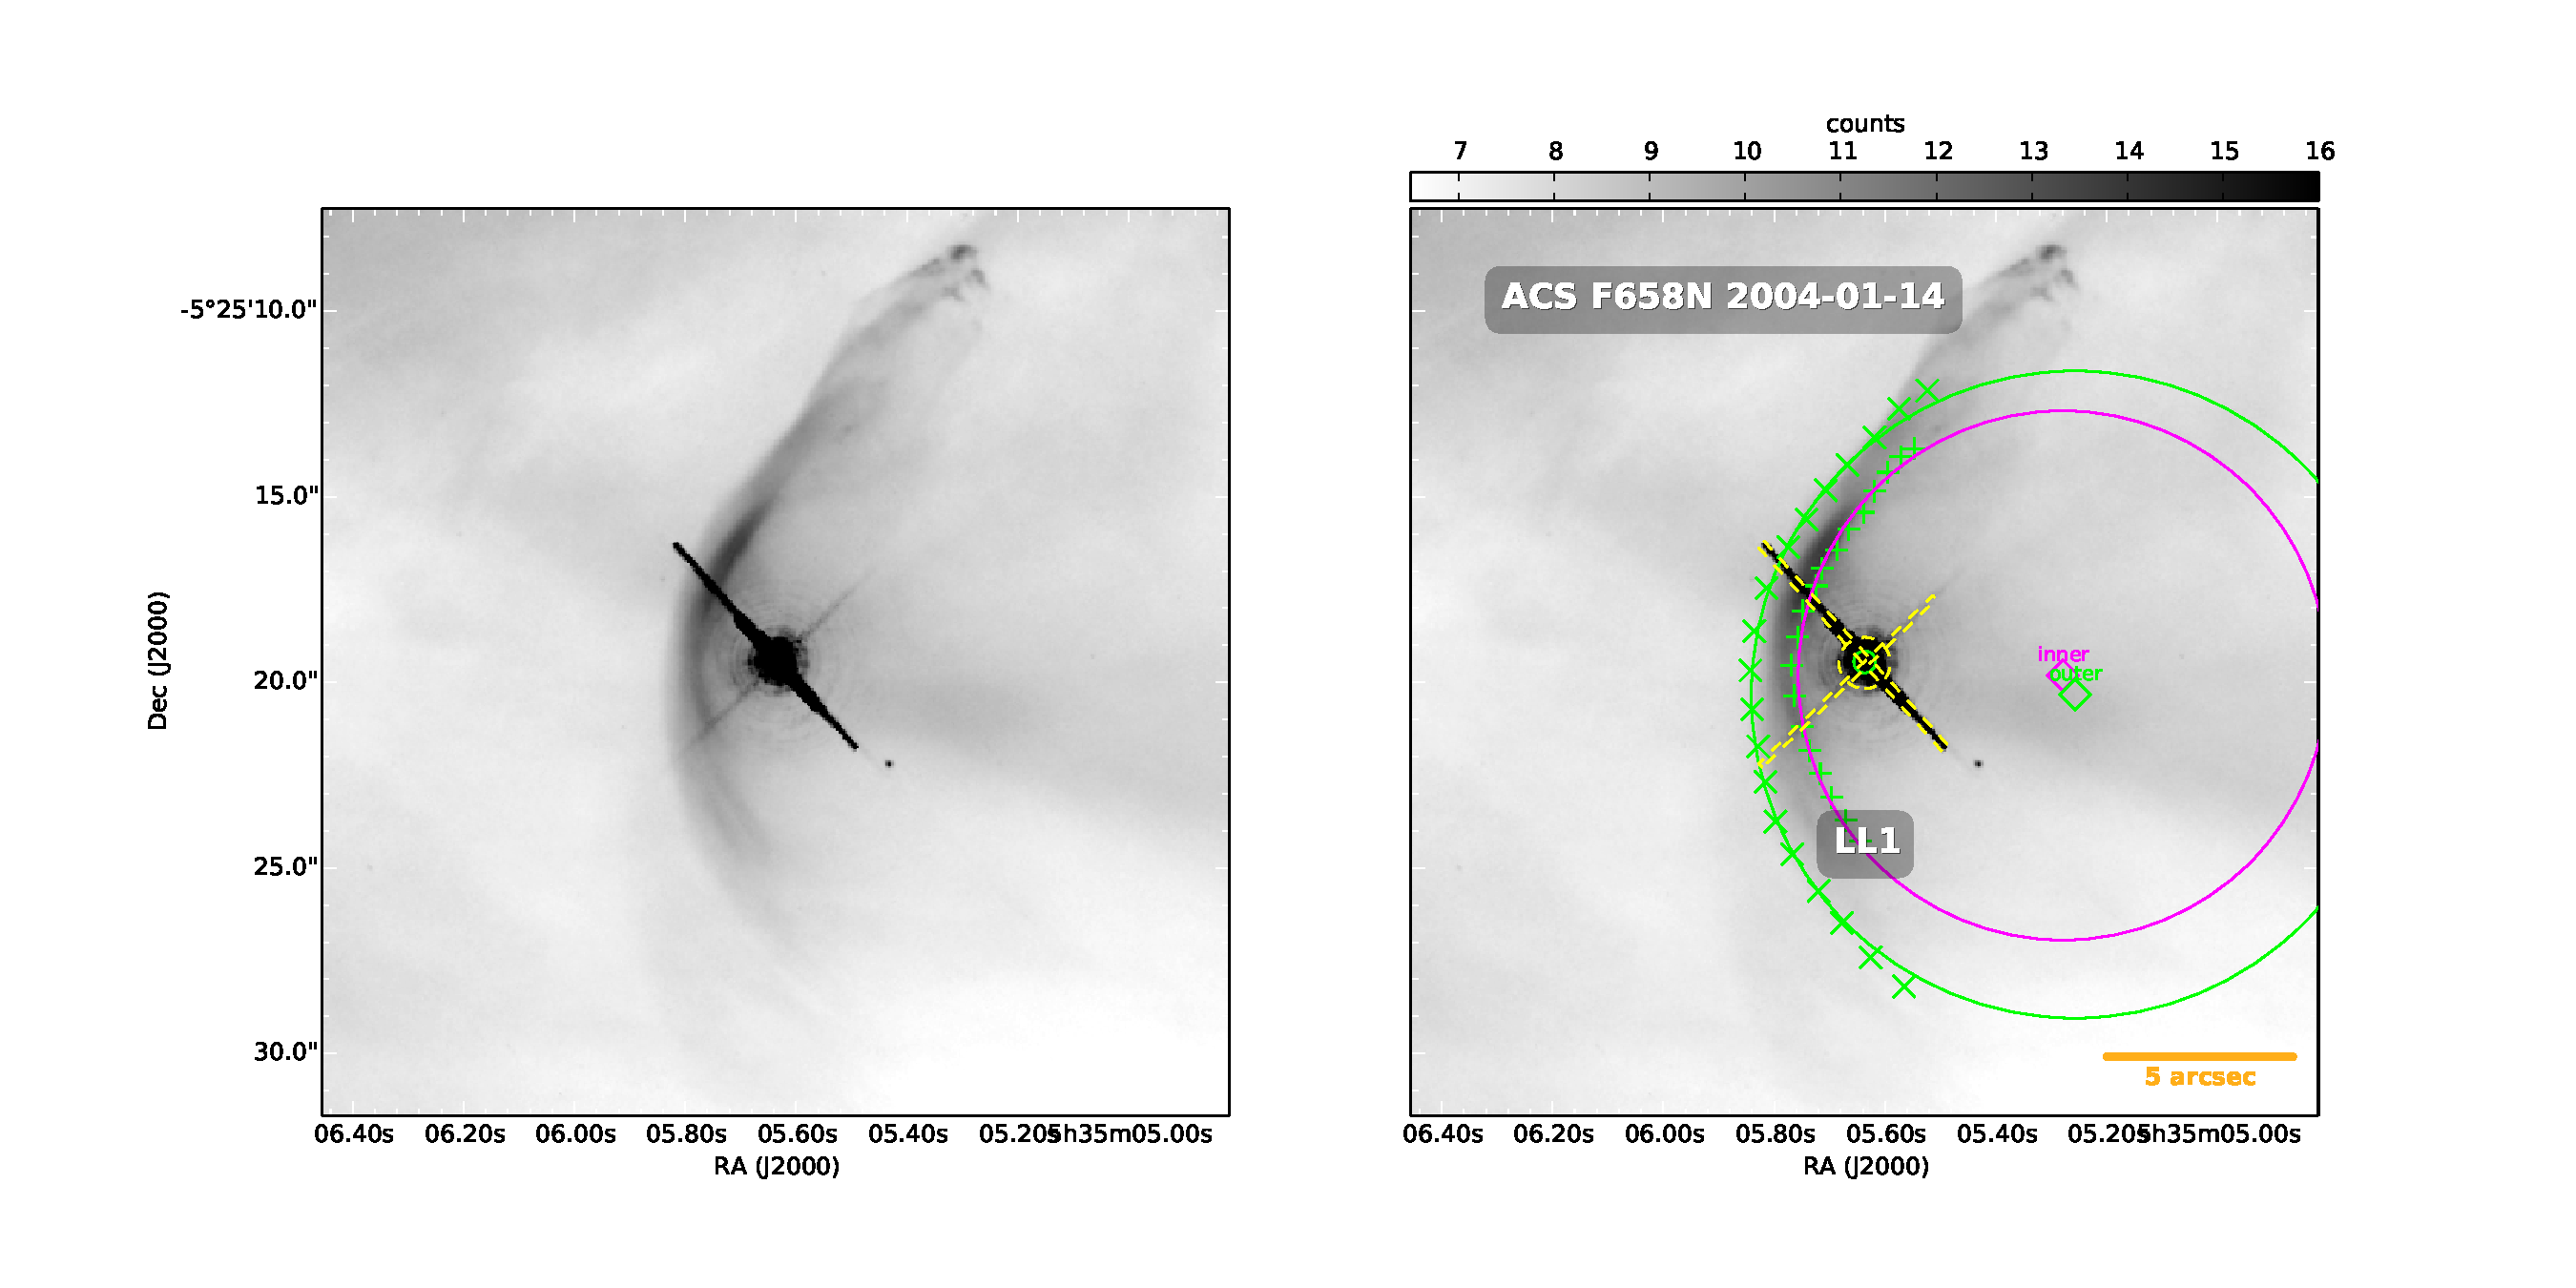
\includegraphics[width=\figwidth,  trim=60 50 100 50, clip]{j8oc01010_wcs/LL1-Bally_01-images.pdf}}\\ 
    \framebox{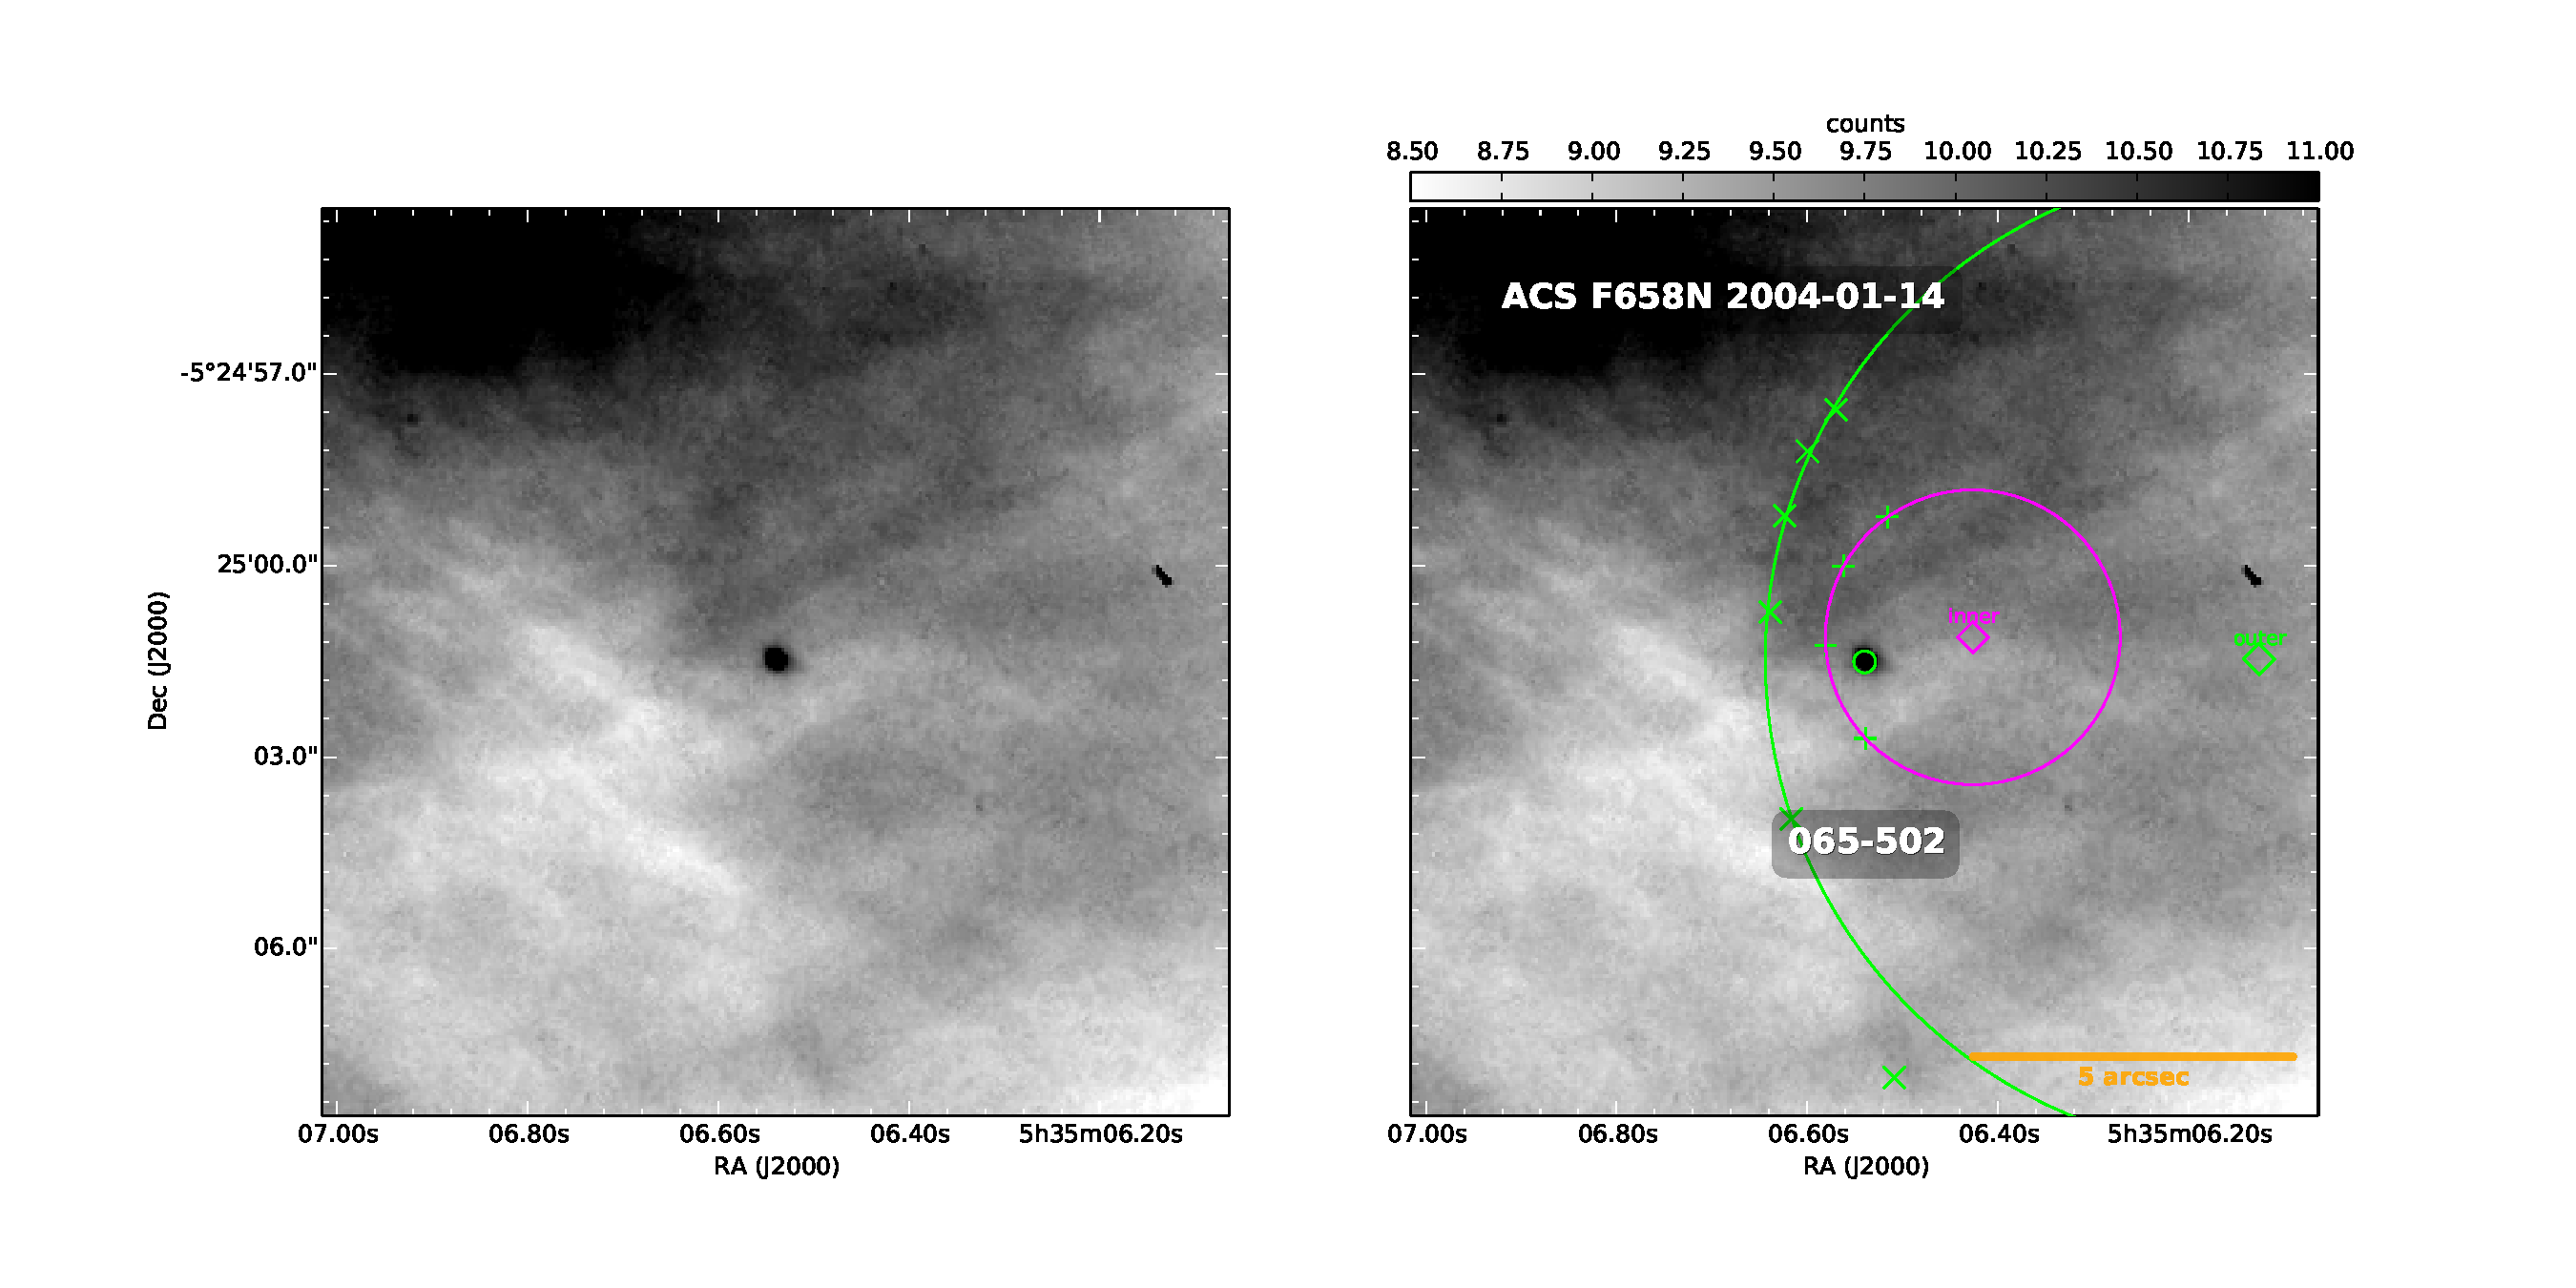
\includegraphics[width=\figwidth,  trim=60 50 100 50, clip]{j8oc01010_wcs/065-502-Bally_01-images.pdf}}
    %\includegraphics[width=0.47\linewidth,  trim=60 50 100 50, clip]{j8oc06010_wcs/066-652-Bally_06-images.pdf}%
   &\framebox{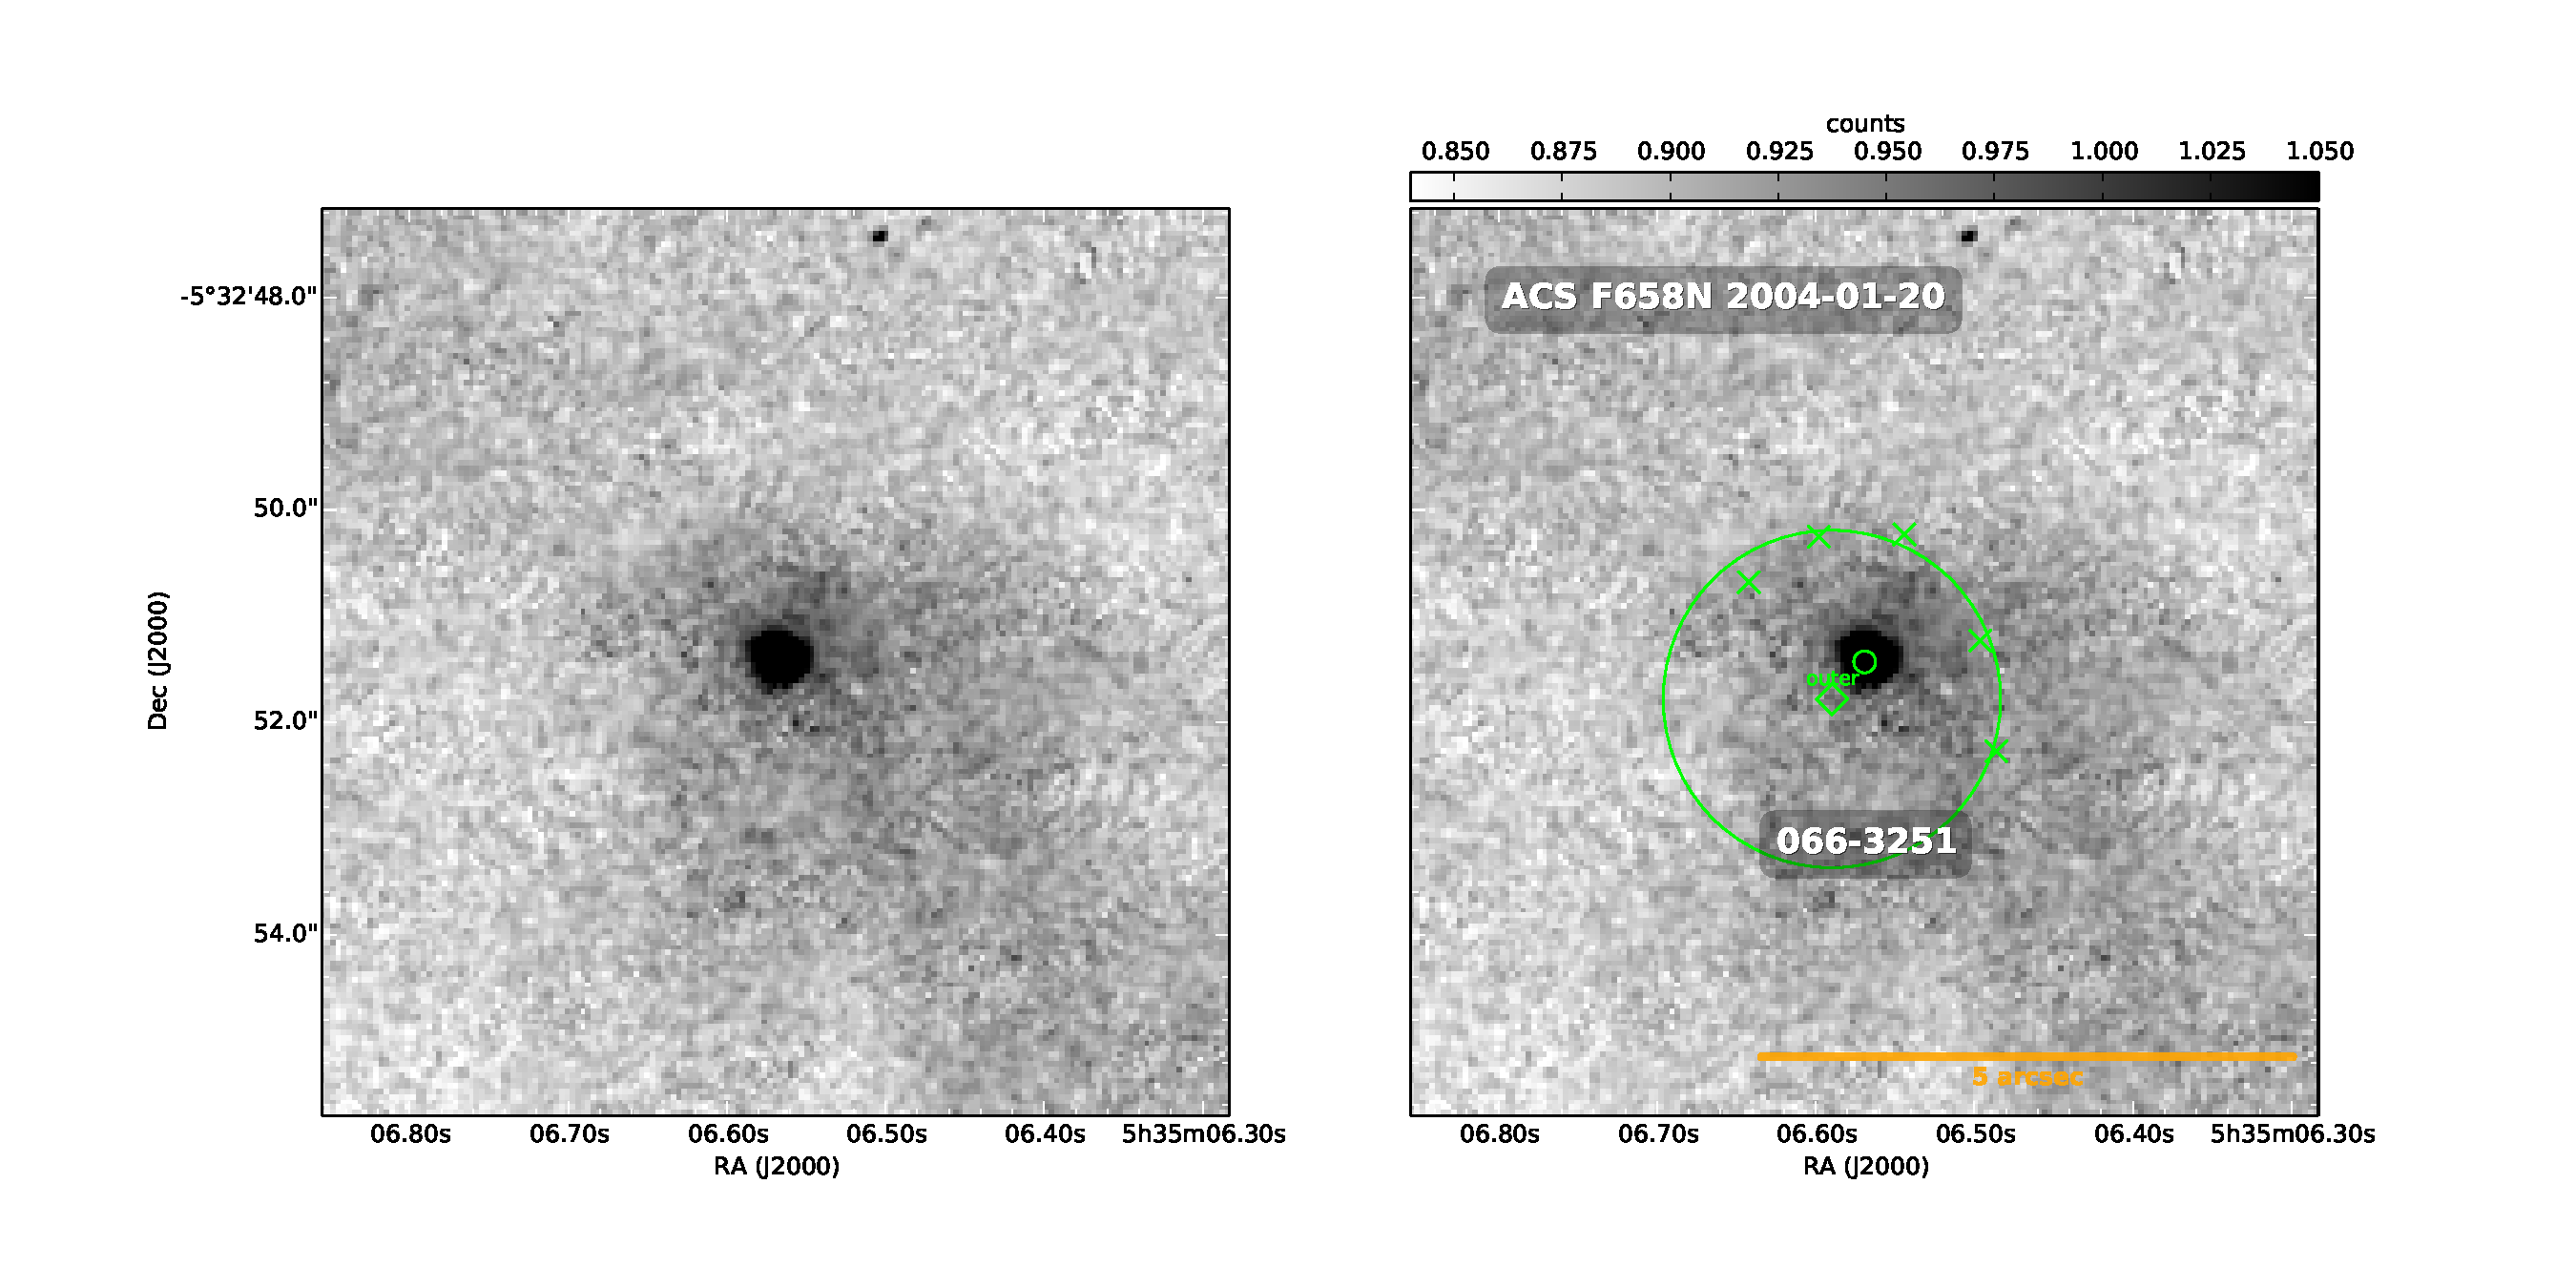
\includegraphics[width=\figwidth,  trim=60 50 90 50, clip]{j8oc14010_wcs/066-3251-Bally_14-images.pdf}}\\ 
   \framebox{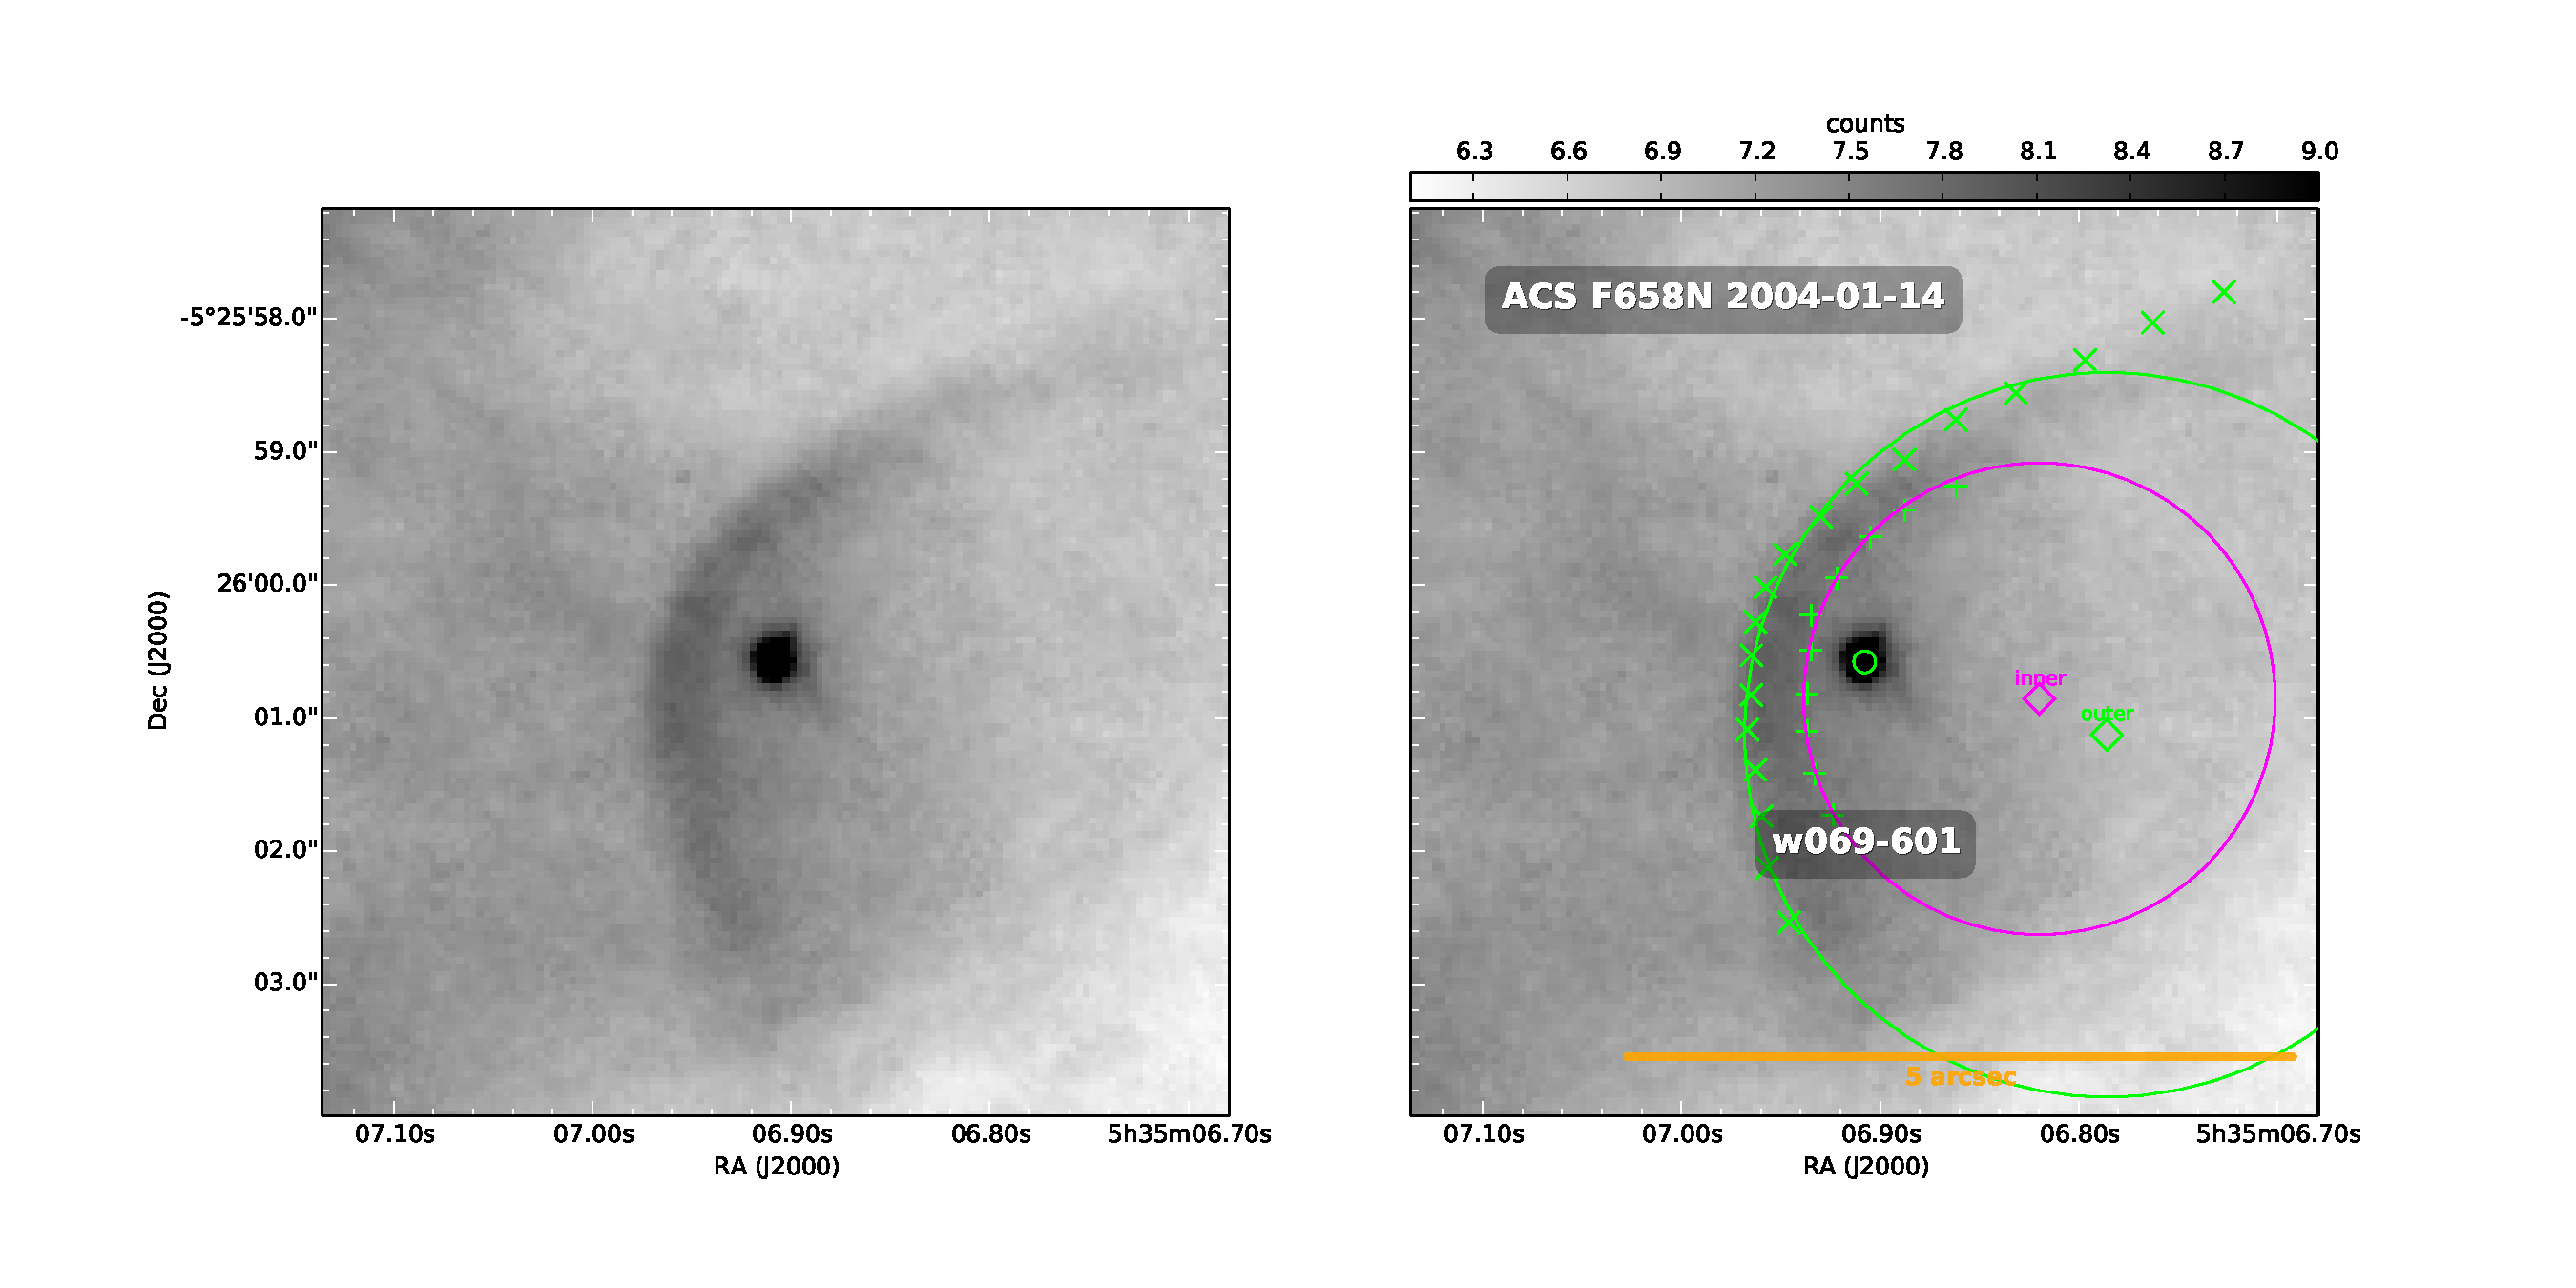
\includegraphics[width=\figwidth,  trim=60 50 100 50, clip]{j8oc01010_wcs/w069-601-Bally_01-images.pdf}}
   &\framebox{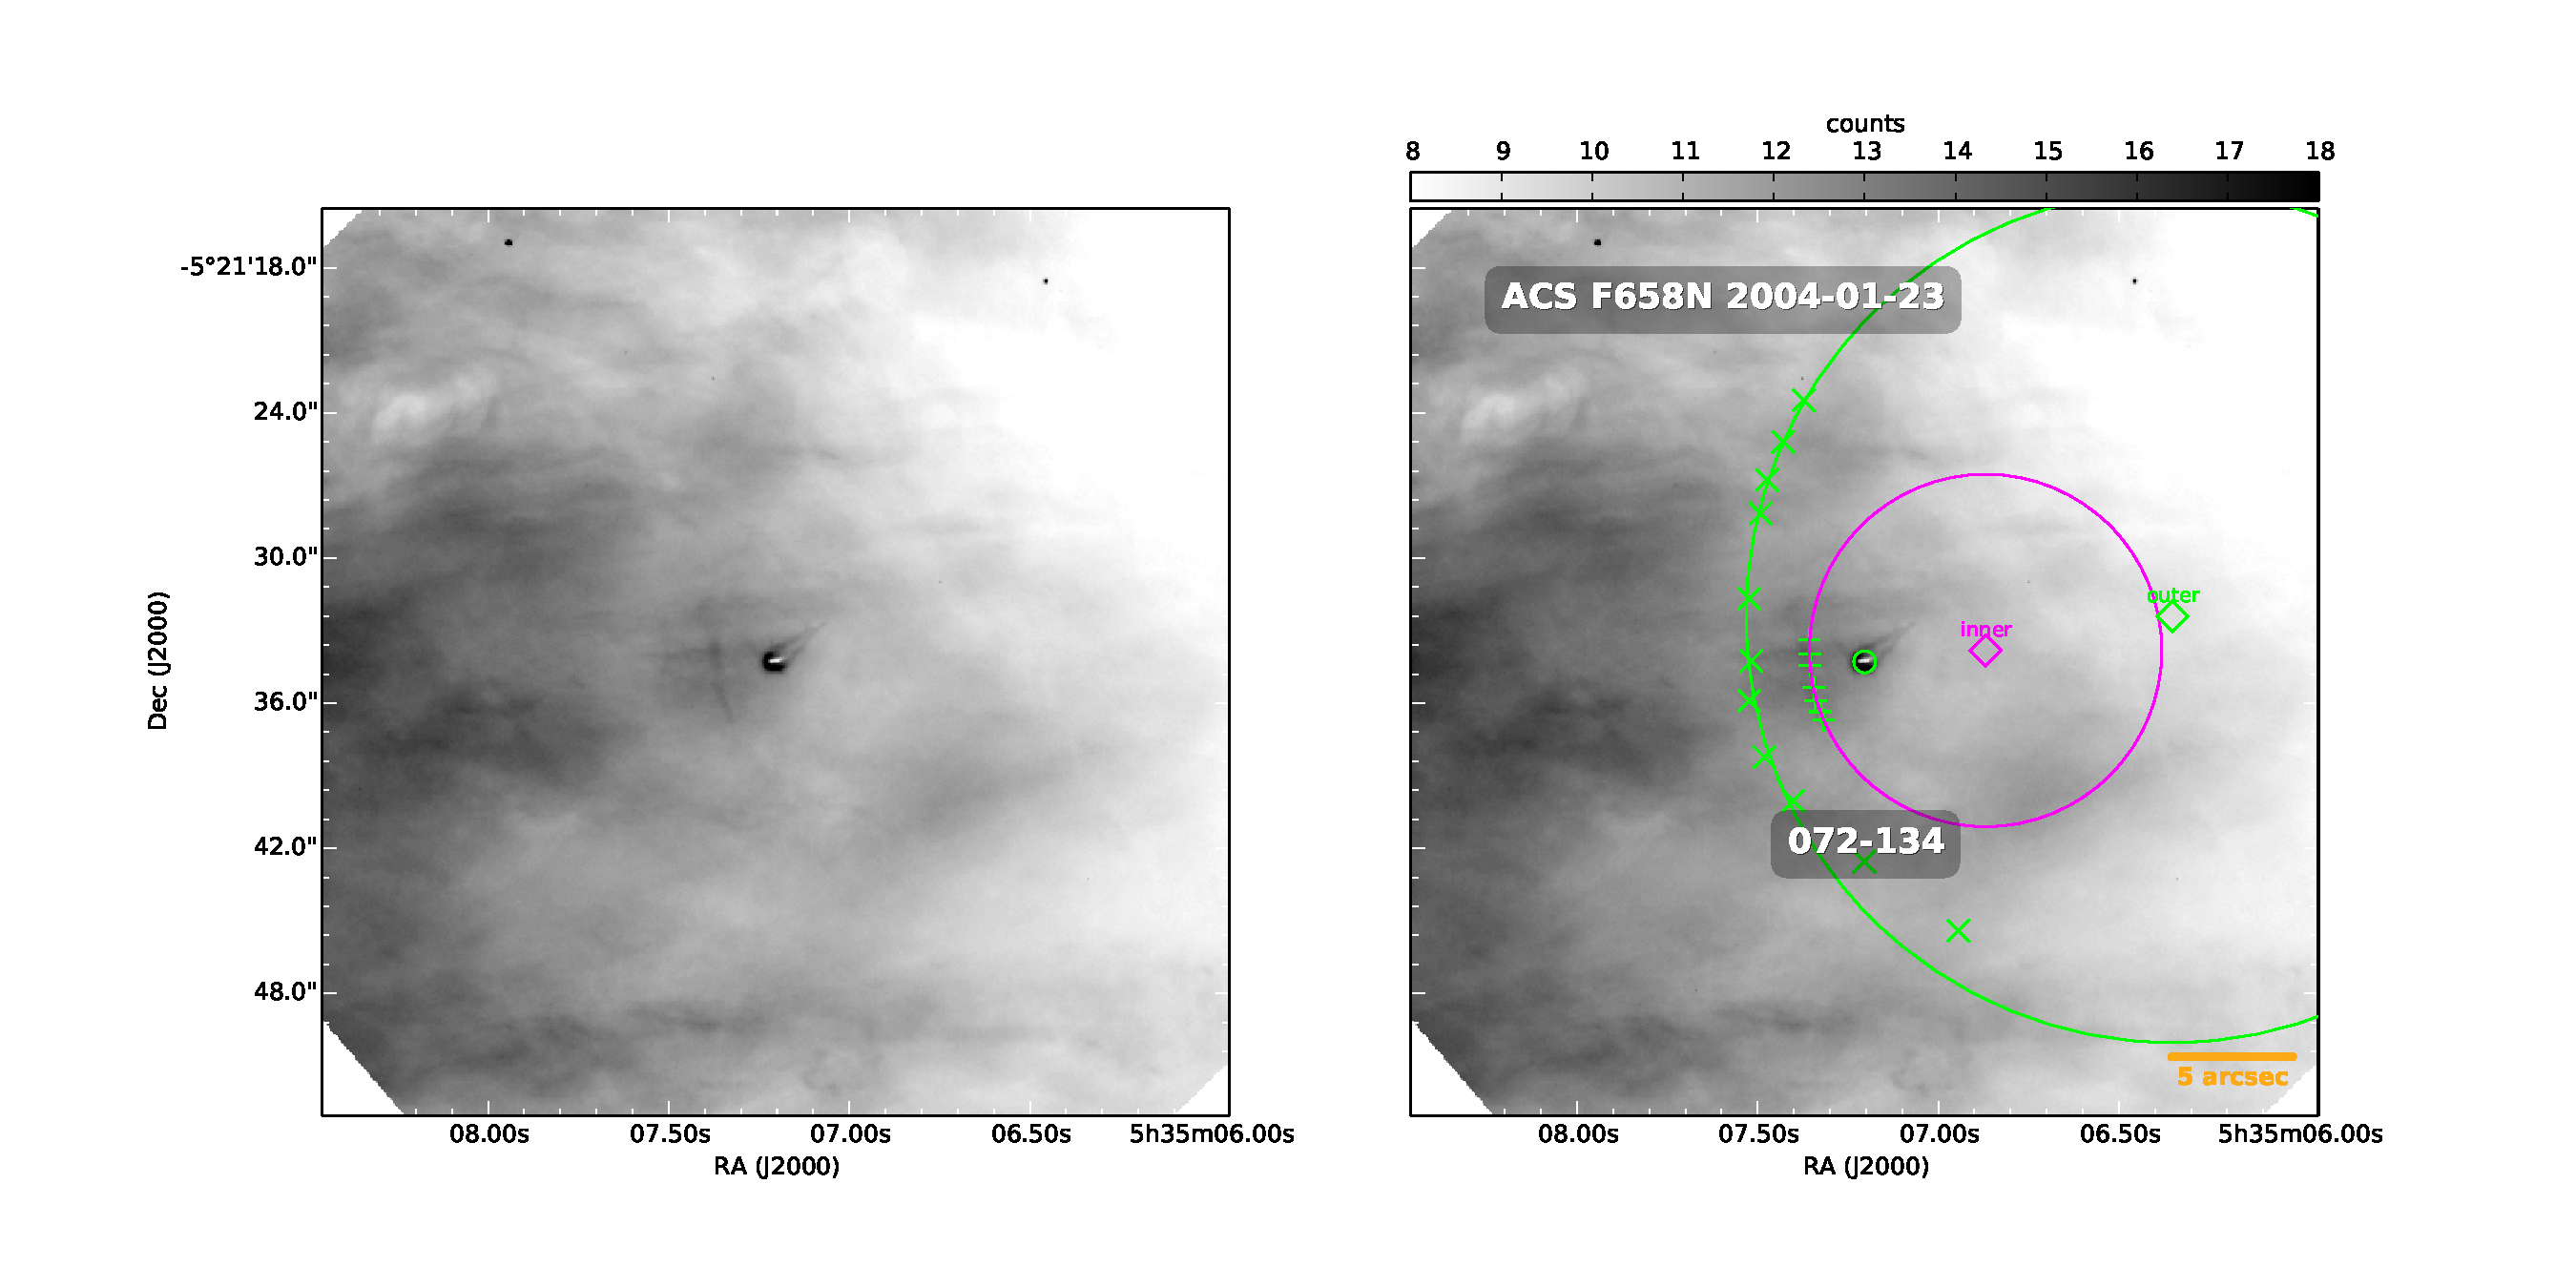
\includegraphics[width=\figwidth,  trim=60 50 100 50, clip]{j8oc09010_wcs/072-134-Bally_09-images.pdf}}\\ 
   \framebox{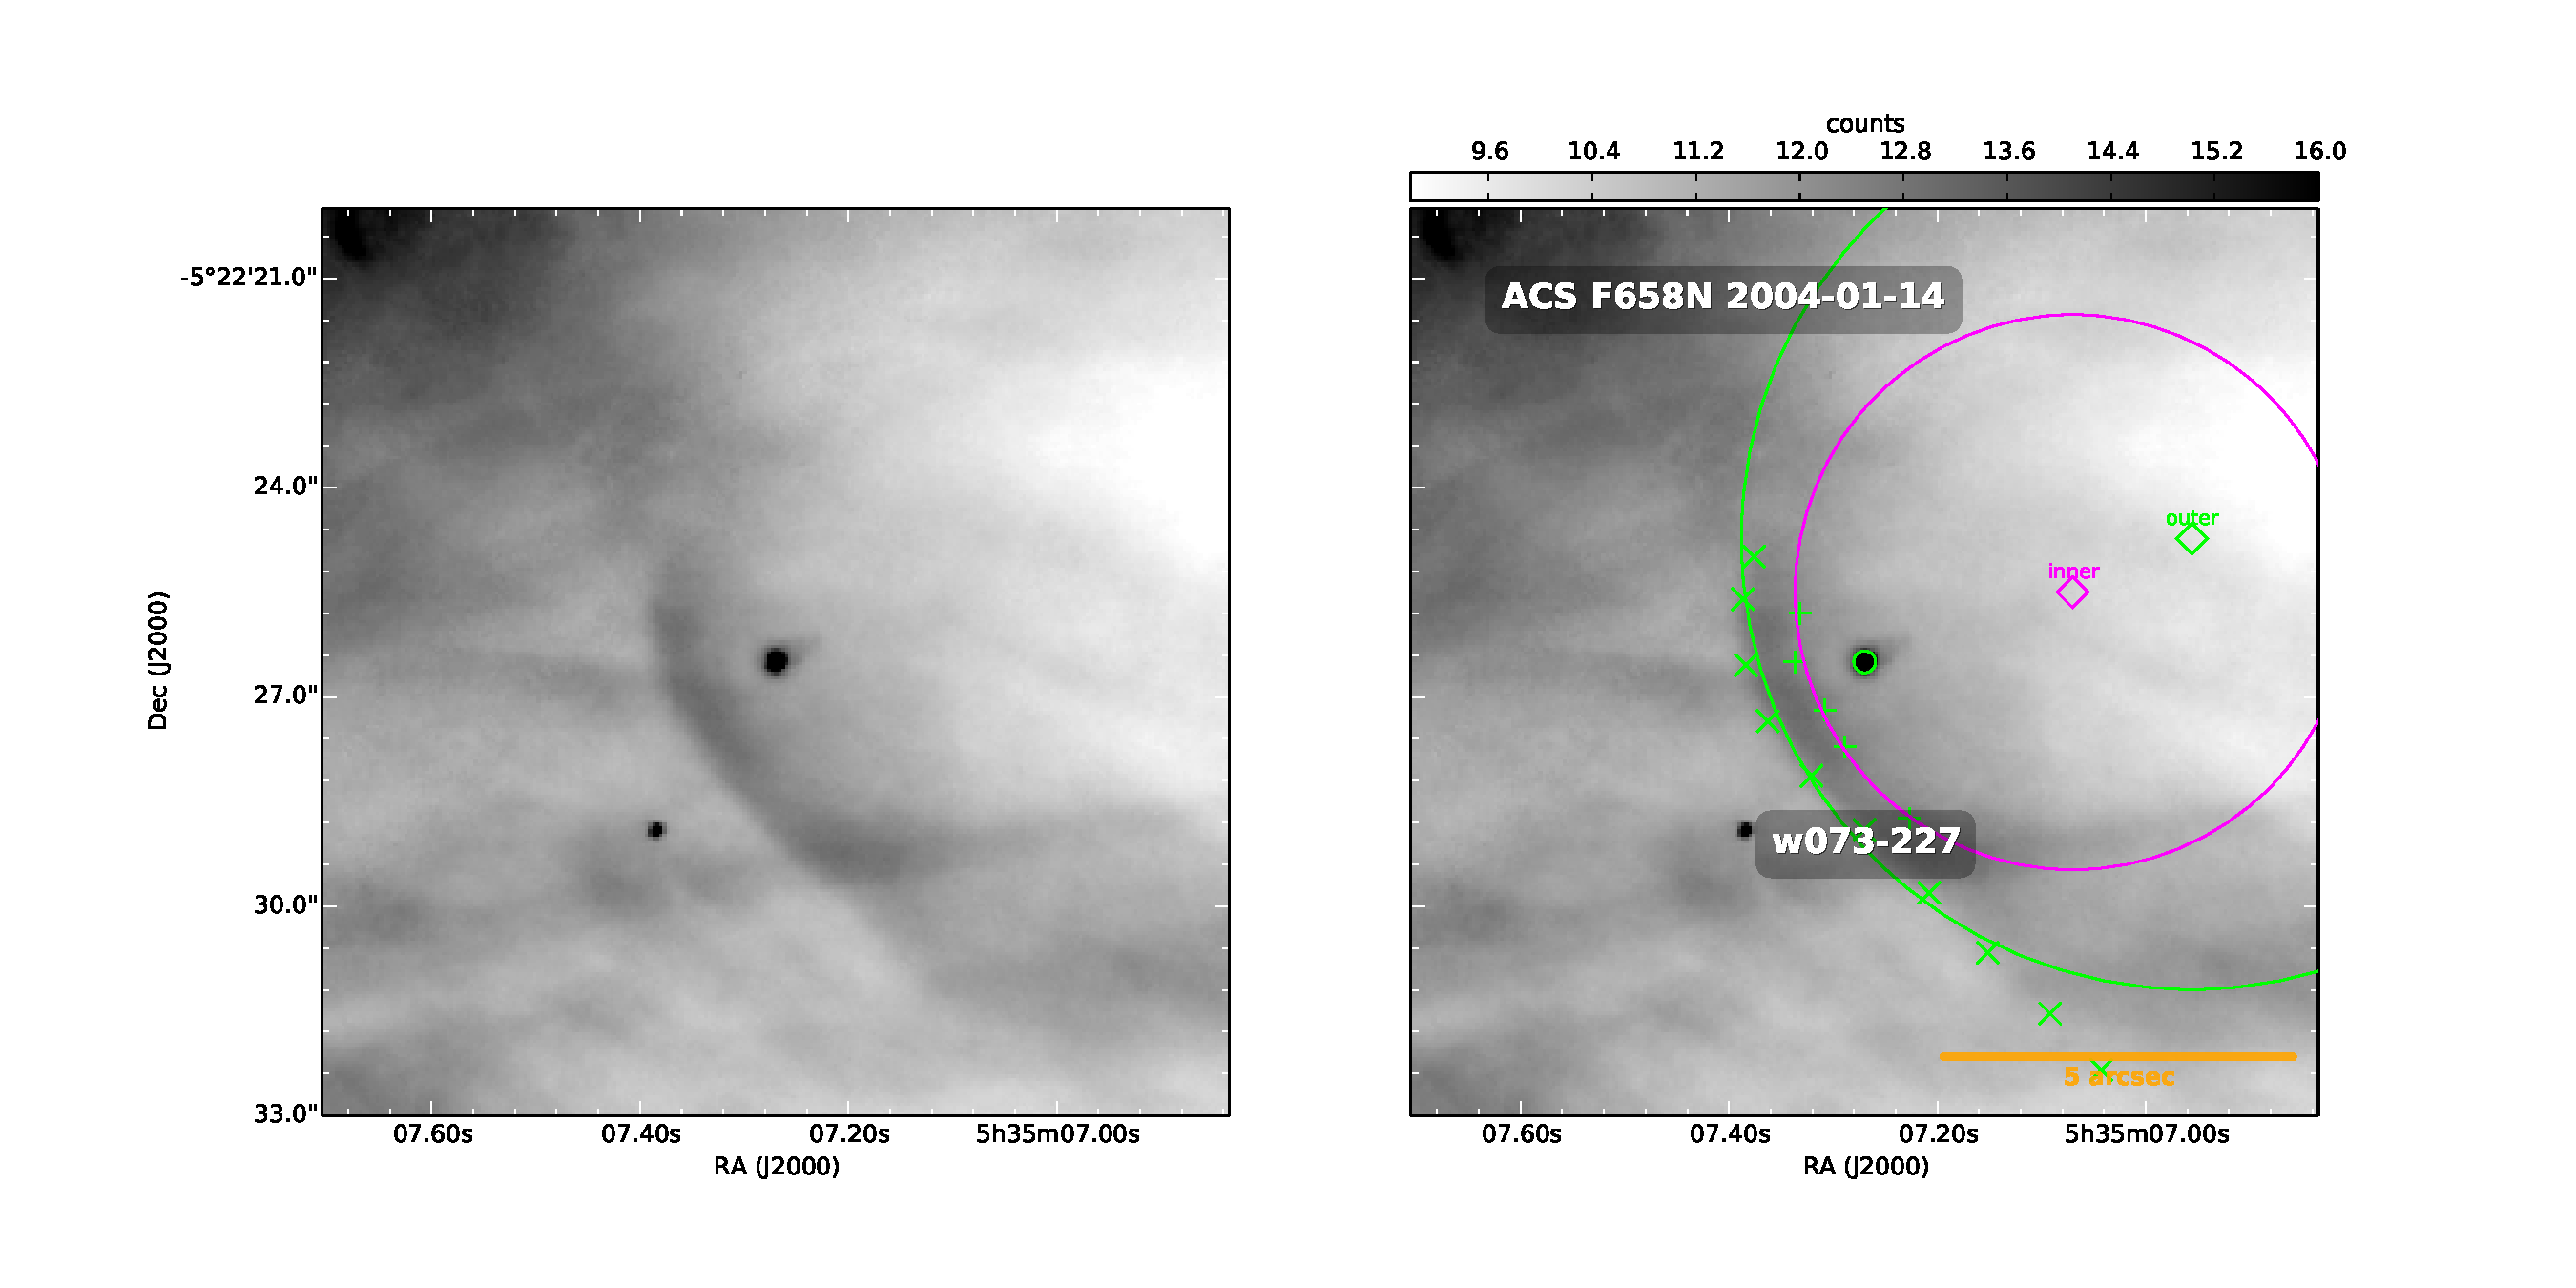
\includegraphics[width=\figwidth,  trim=60 50 100 50, clip]{j8oc01010_wcs/w073-227-Bally_01-images.pdf}}
 &\framebox{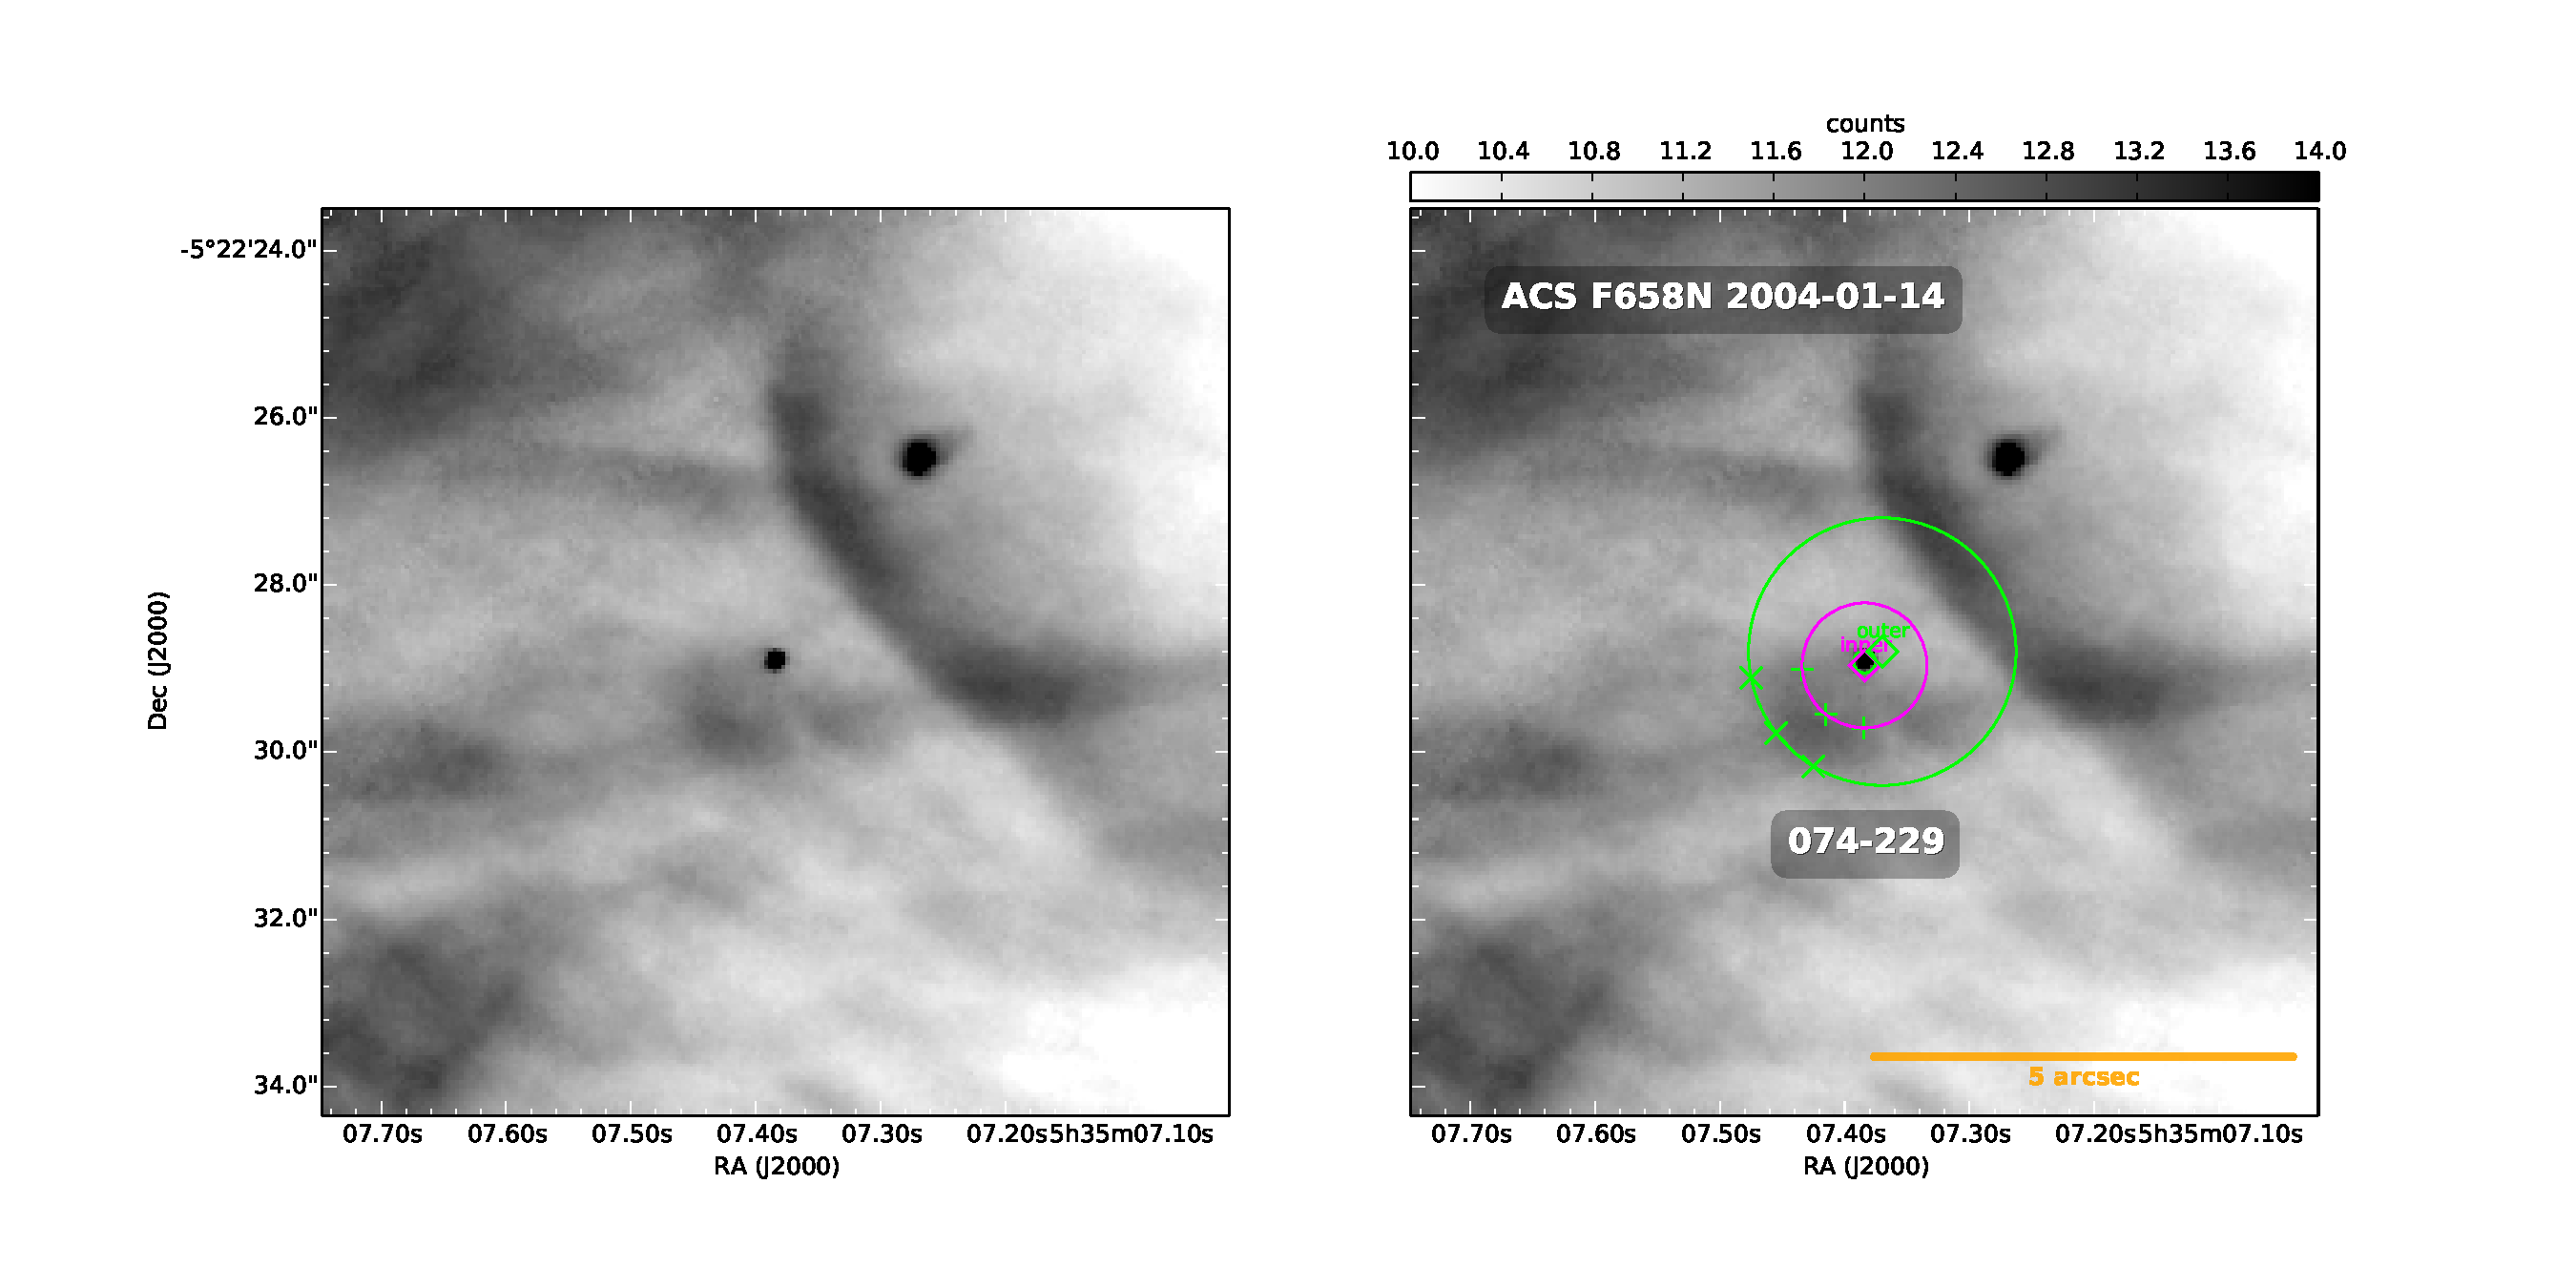
\includegraphics[width=\figwidth,  trim=60 50 100 50, clip]{j8oc01010_wcs/074-229-Bally_01-images.pdf}}\\ 
\end{tabular}
\end{figure*} 

\begin{figure*}
\setlength\tabcolsep{1.5pt}
\begin{tabular}{l l} 
  \framebox{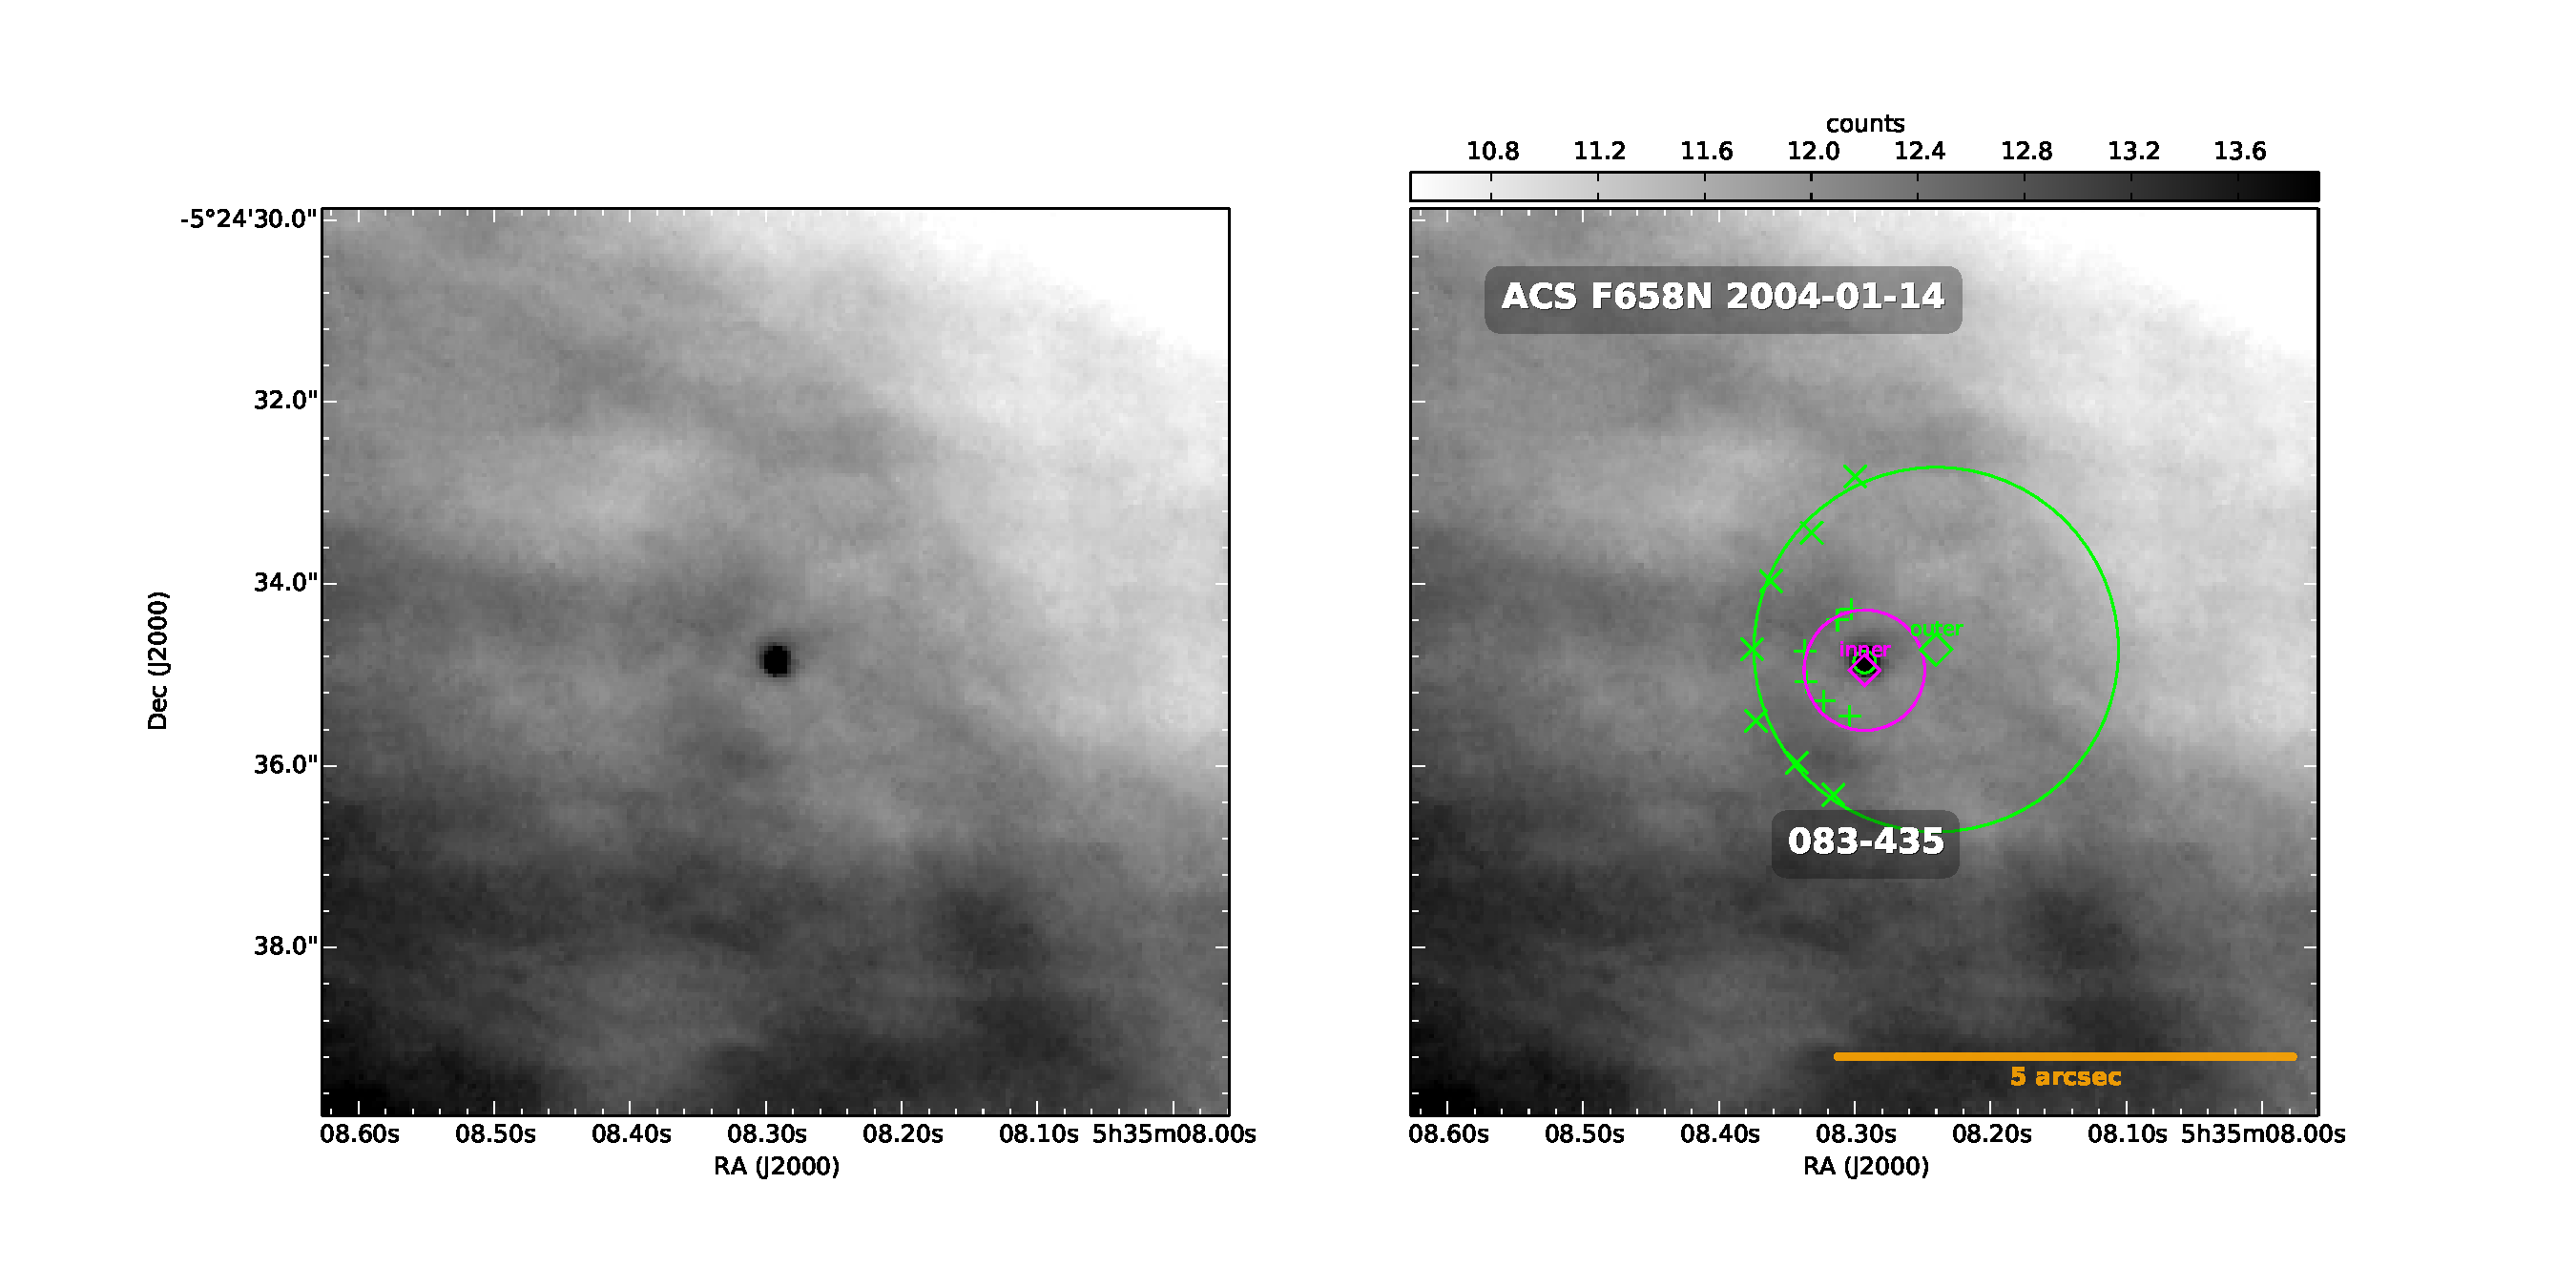
\includegraphics[width=\figwidth,  trim=60 50 100 50, clip]{j8oc01010_wcs/083-435-Bally_01-images.pdf}}
    &\framebox{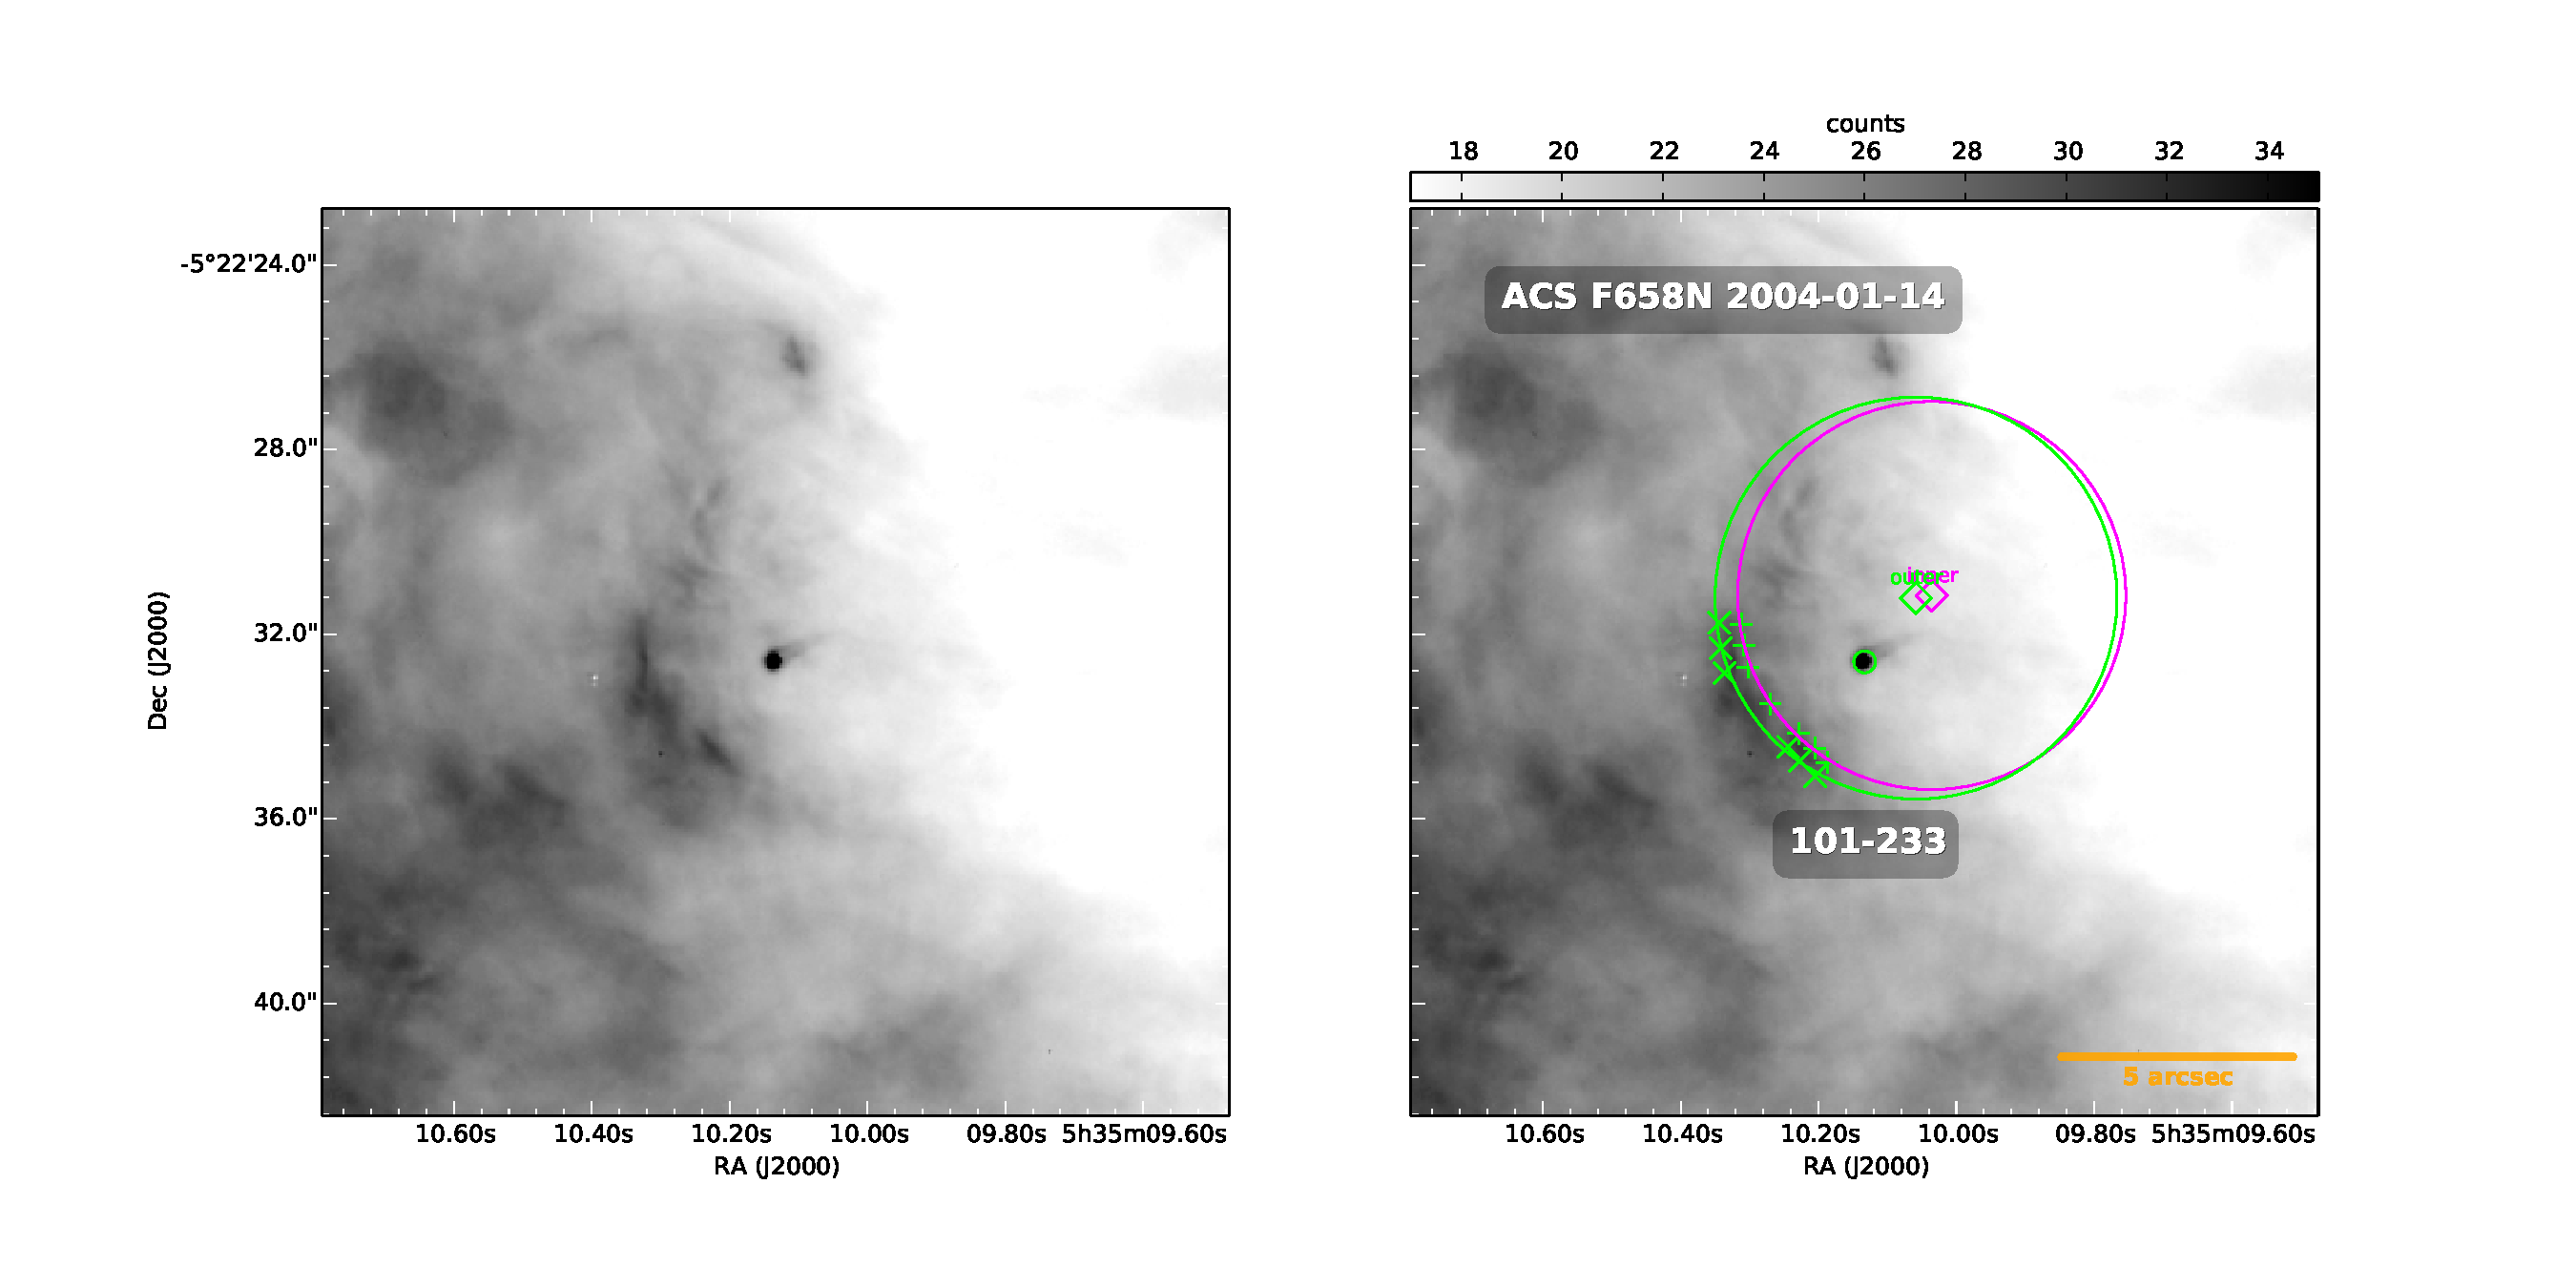
\includegraphics[width=\figwidth,  trim=60 50 100 50, clip]{j8oc01010_wcs/101-233-Bally_01-images.pdf}}\\
   \framebox{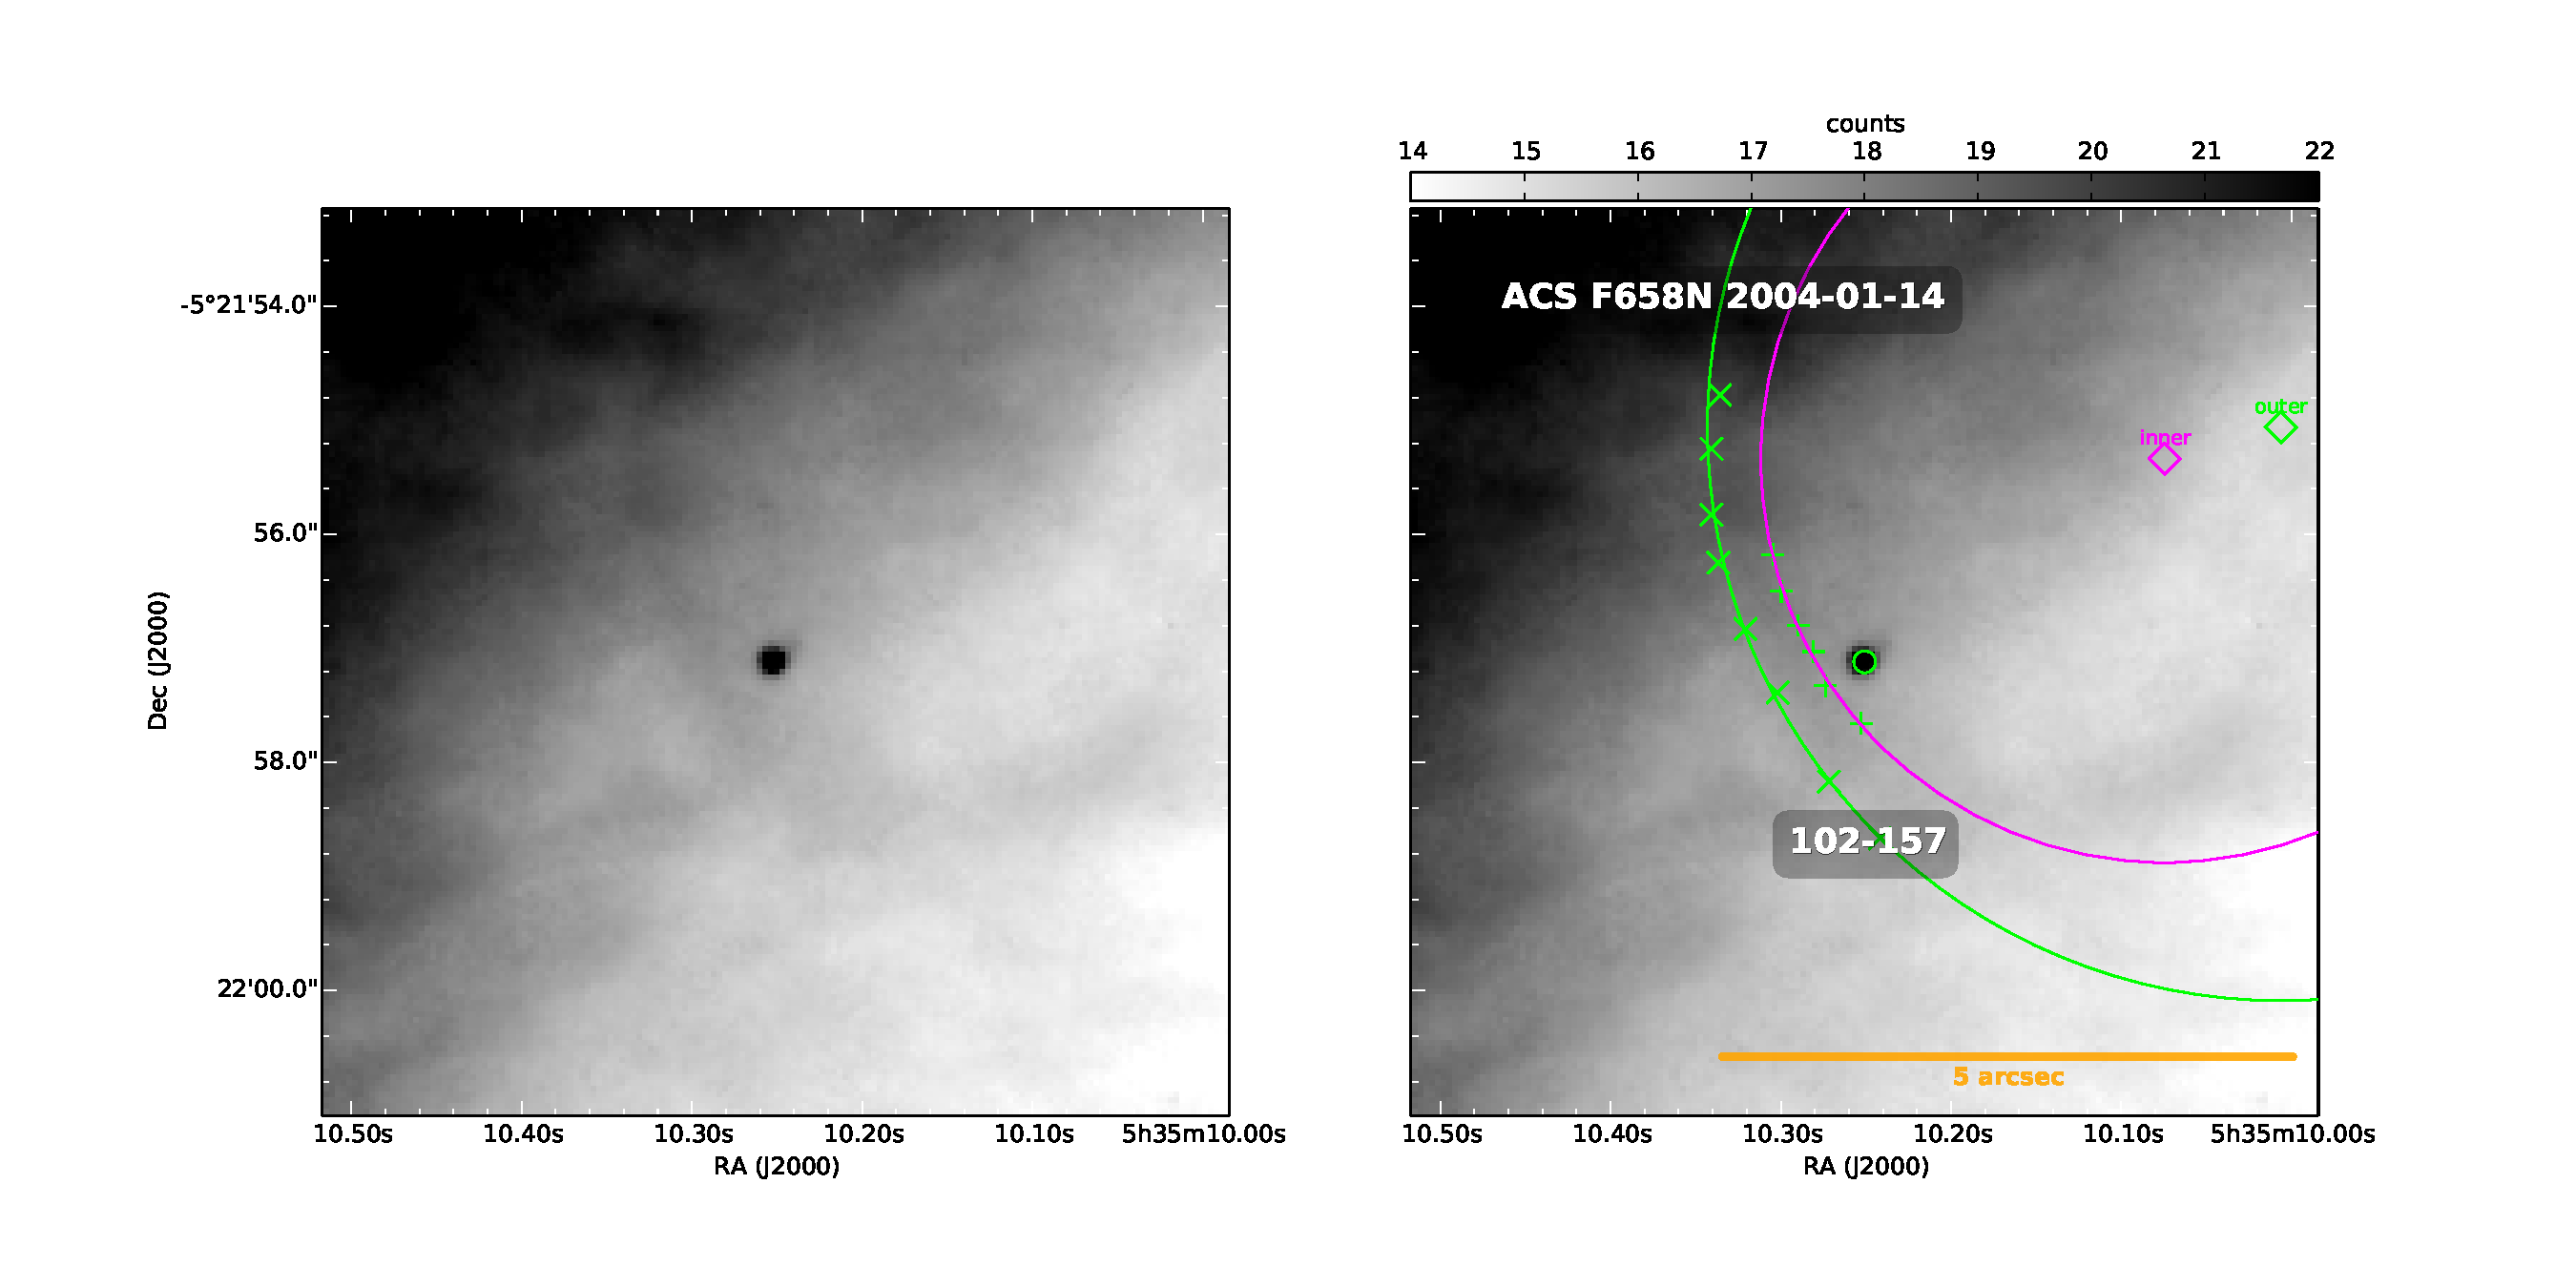
\includegraphics[width=\figwidth,  trim=60 50 100 50, clip]{j8oc01010_wcs/102-157-Bally_01-images.pdf}}
   &\framebox{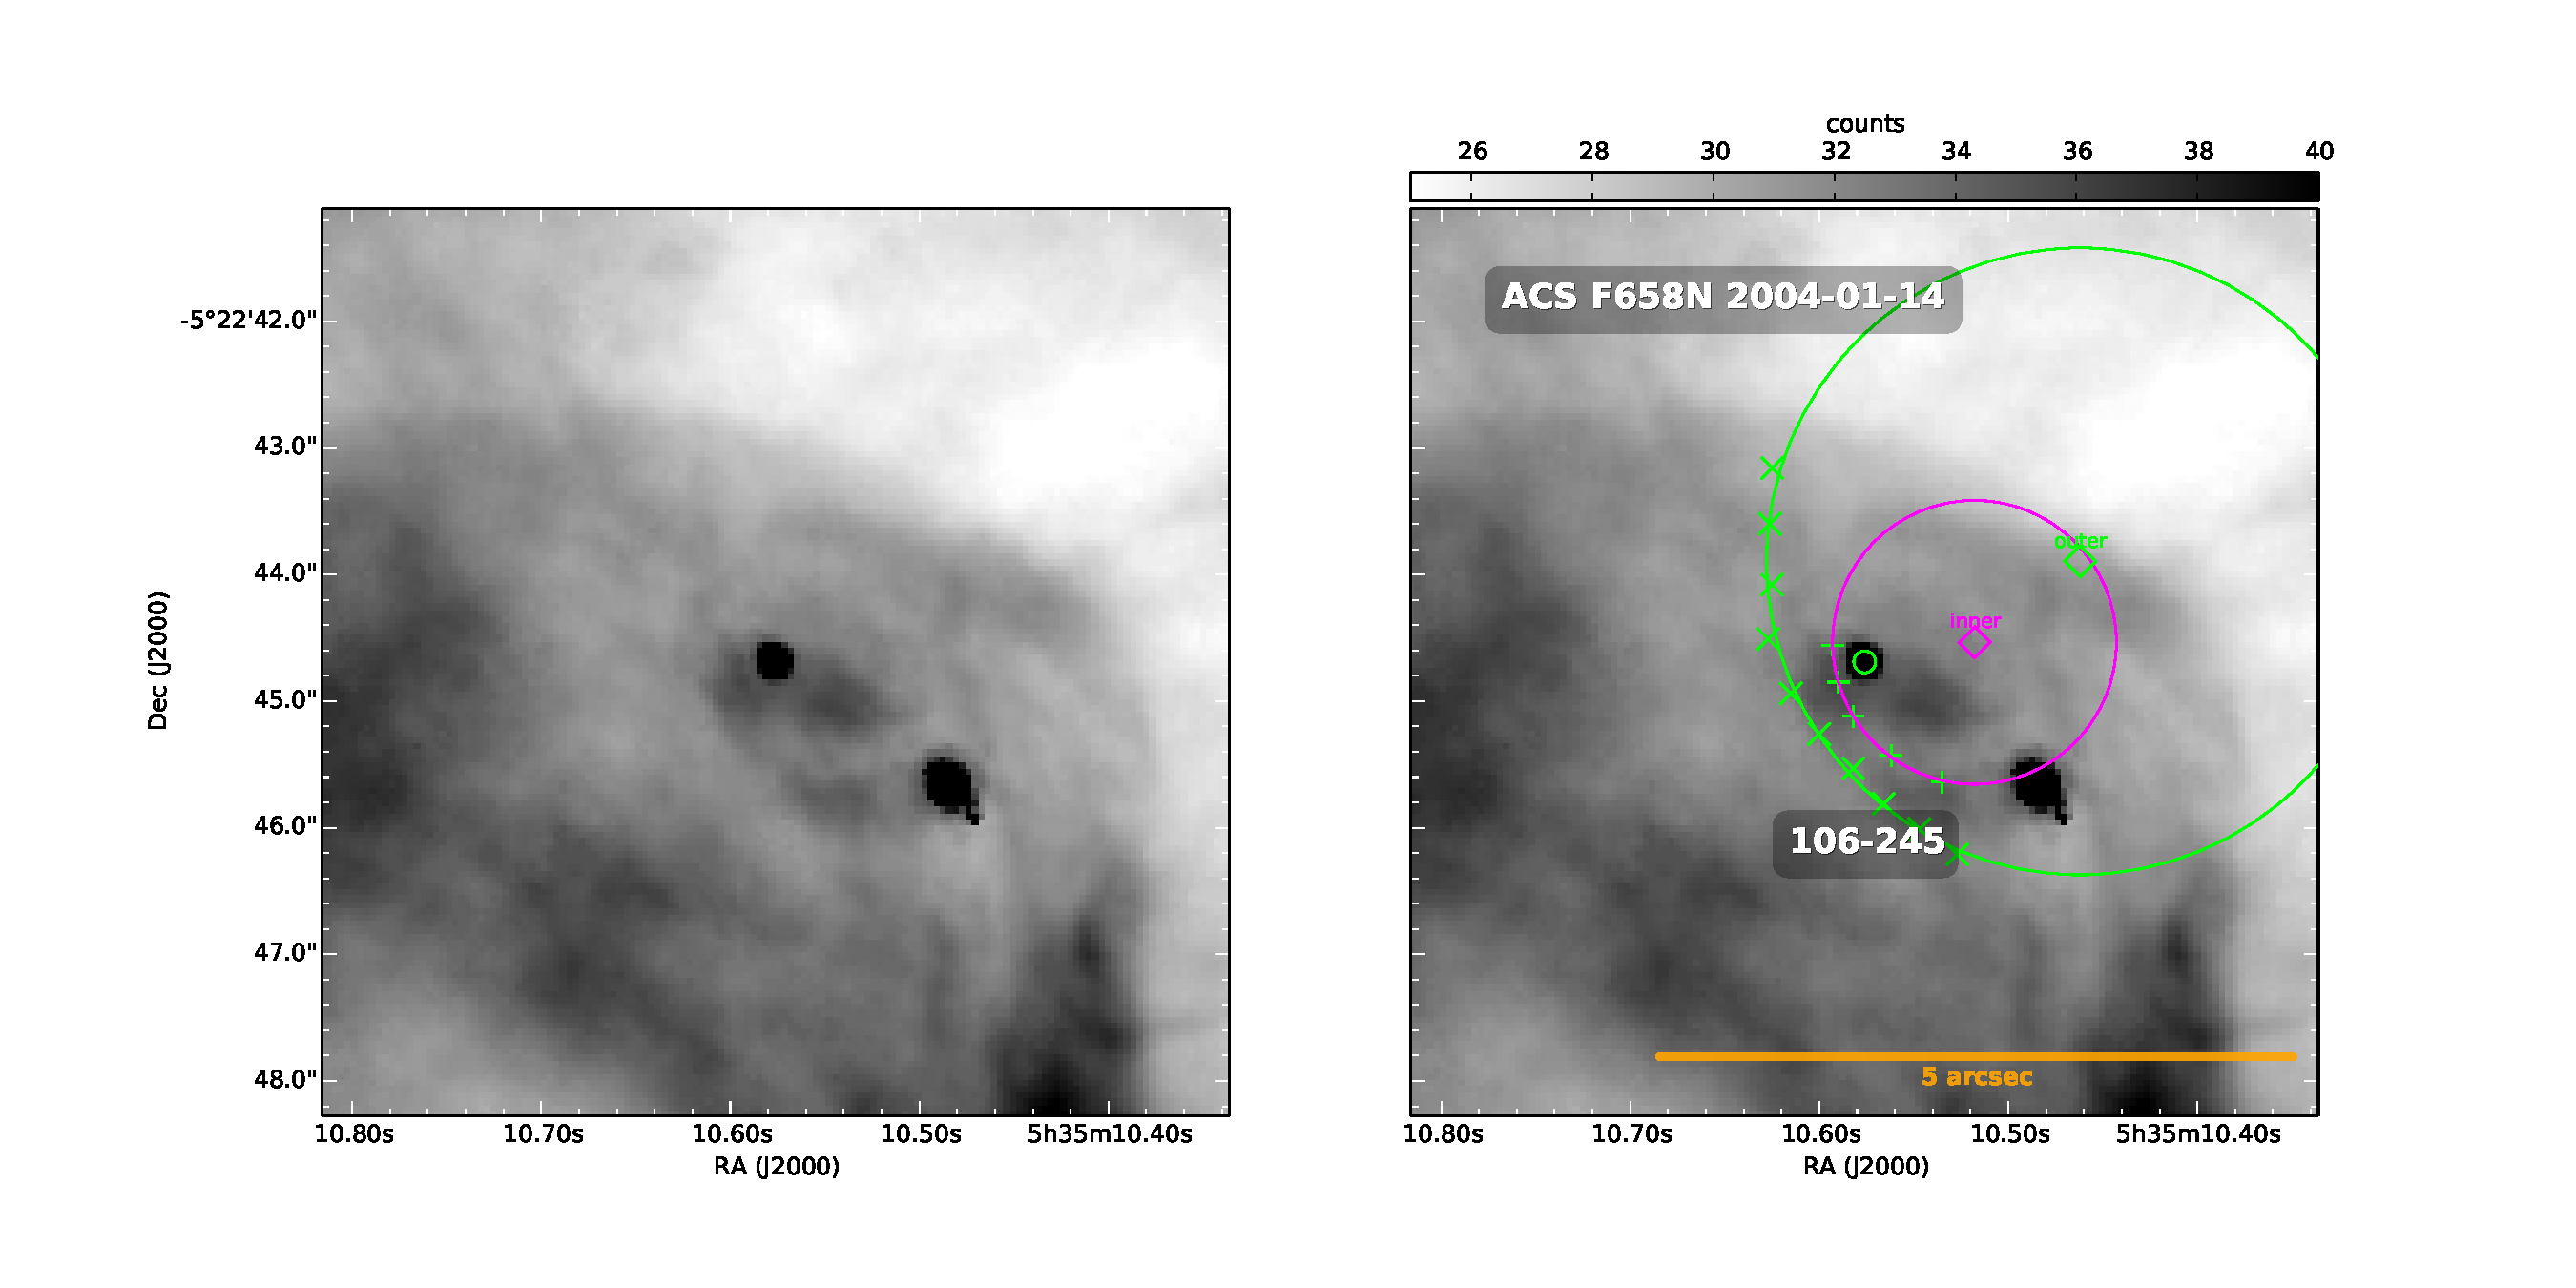
\includegraphics[width=\figwidth,  trim=60 50 100 50, clip]{j8oc01010_wcs/106-245-Bally_01-images.pdf}}\\
   \framebox{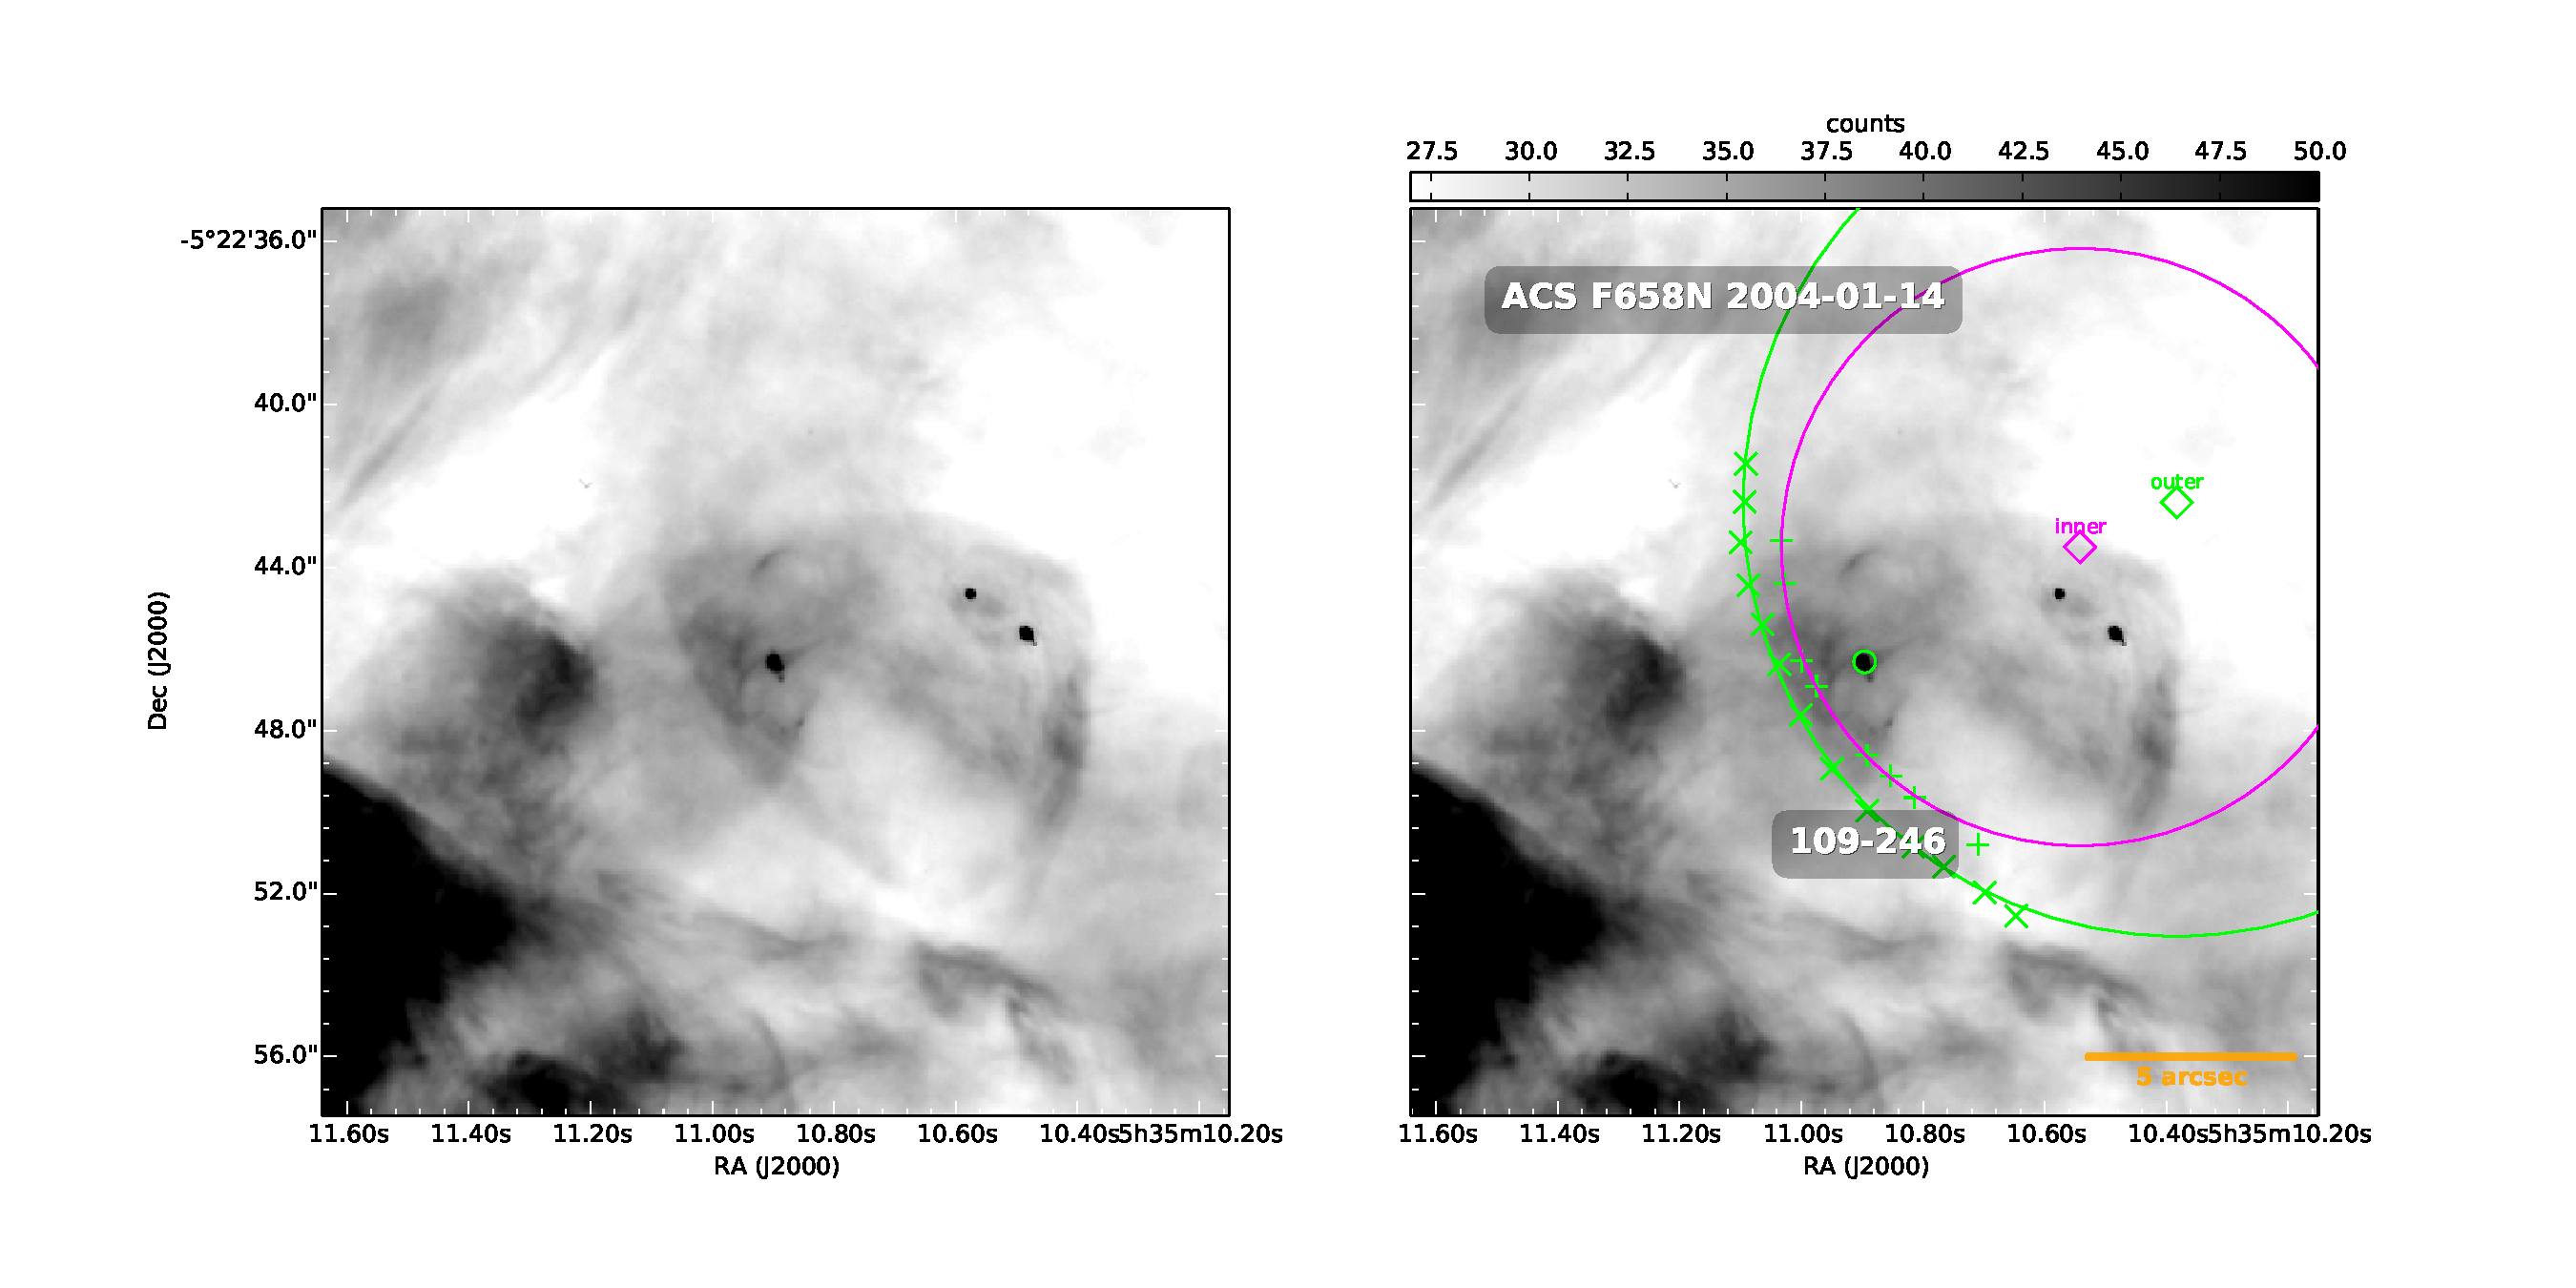
\includegraphics[width=\figwidth,  trim=60 50 100 50, clip]{j8oc01010_wcs/109-246-Bally_01-images.pdf}}
  & \framebox{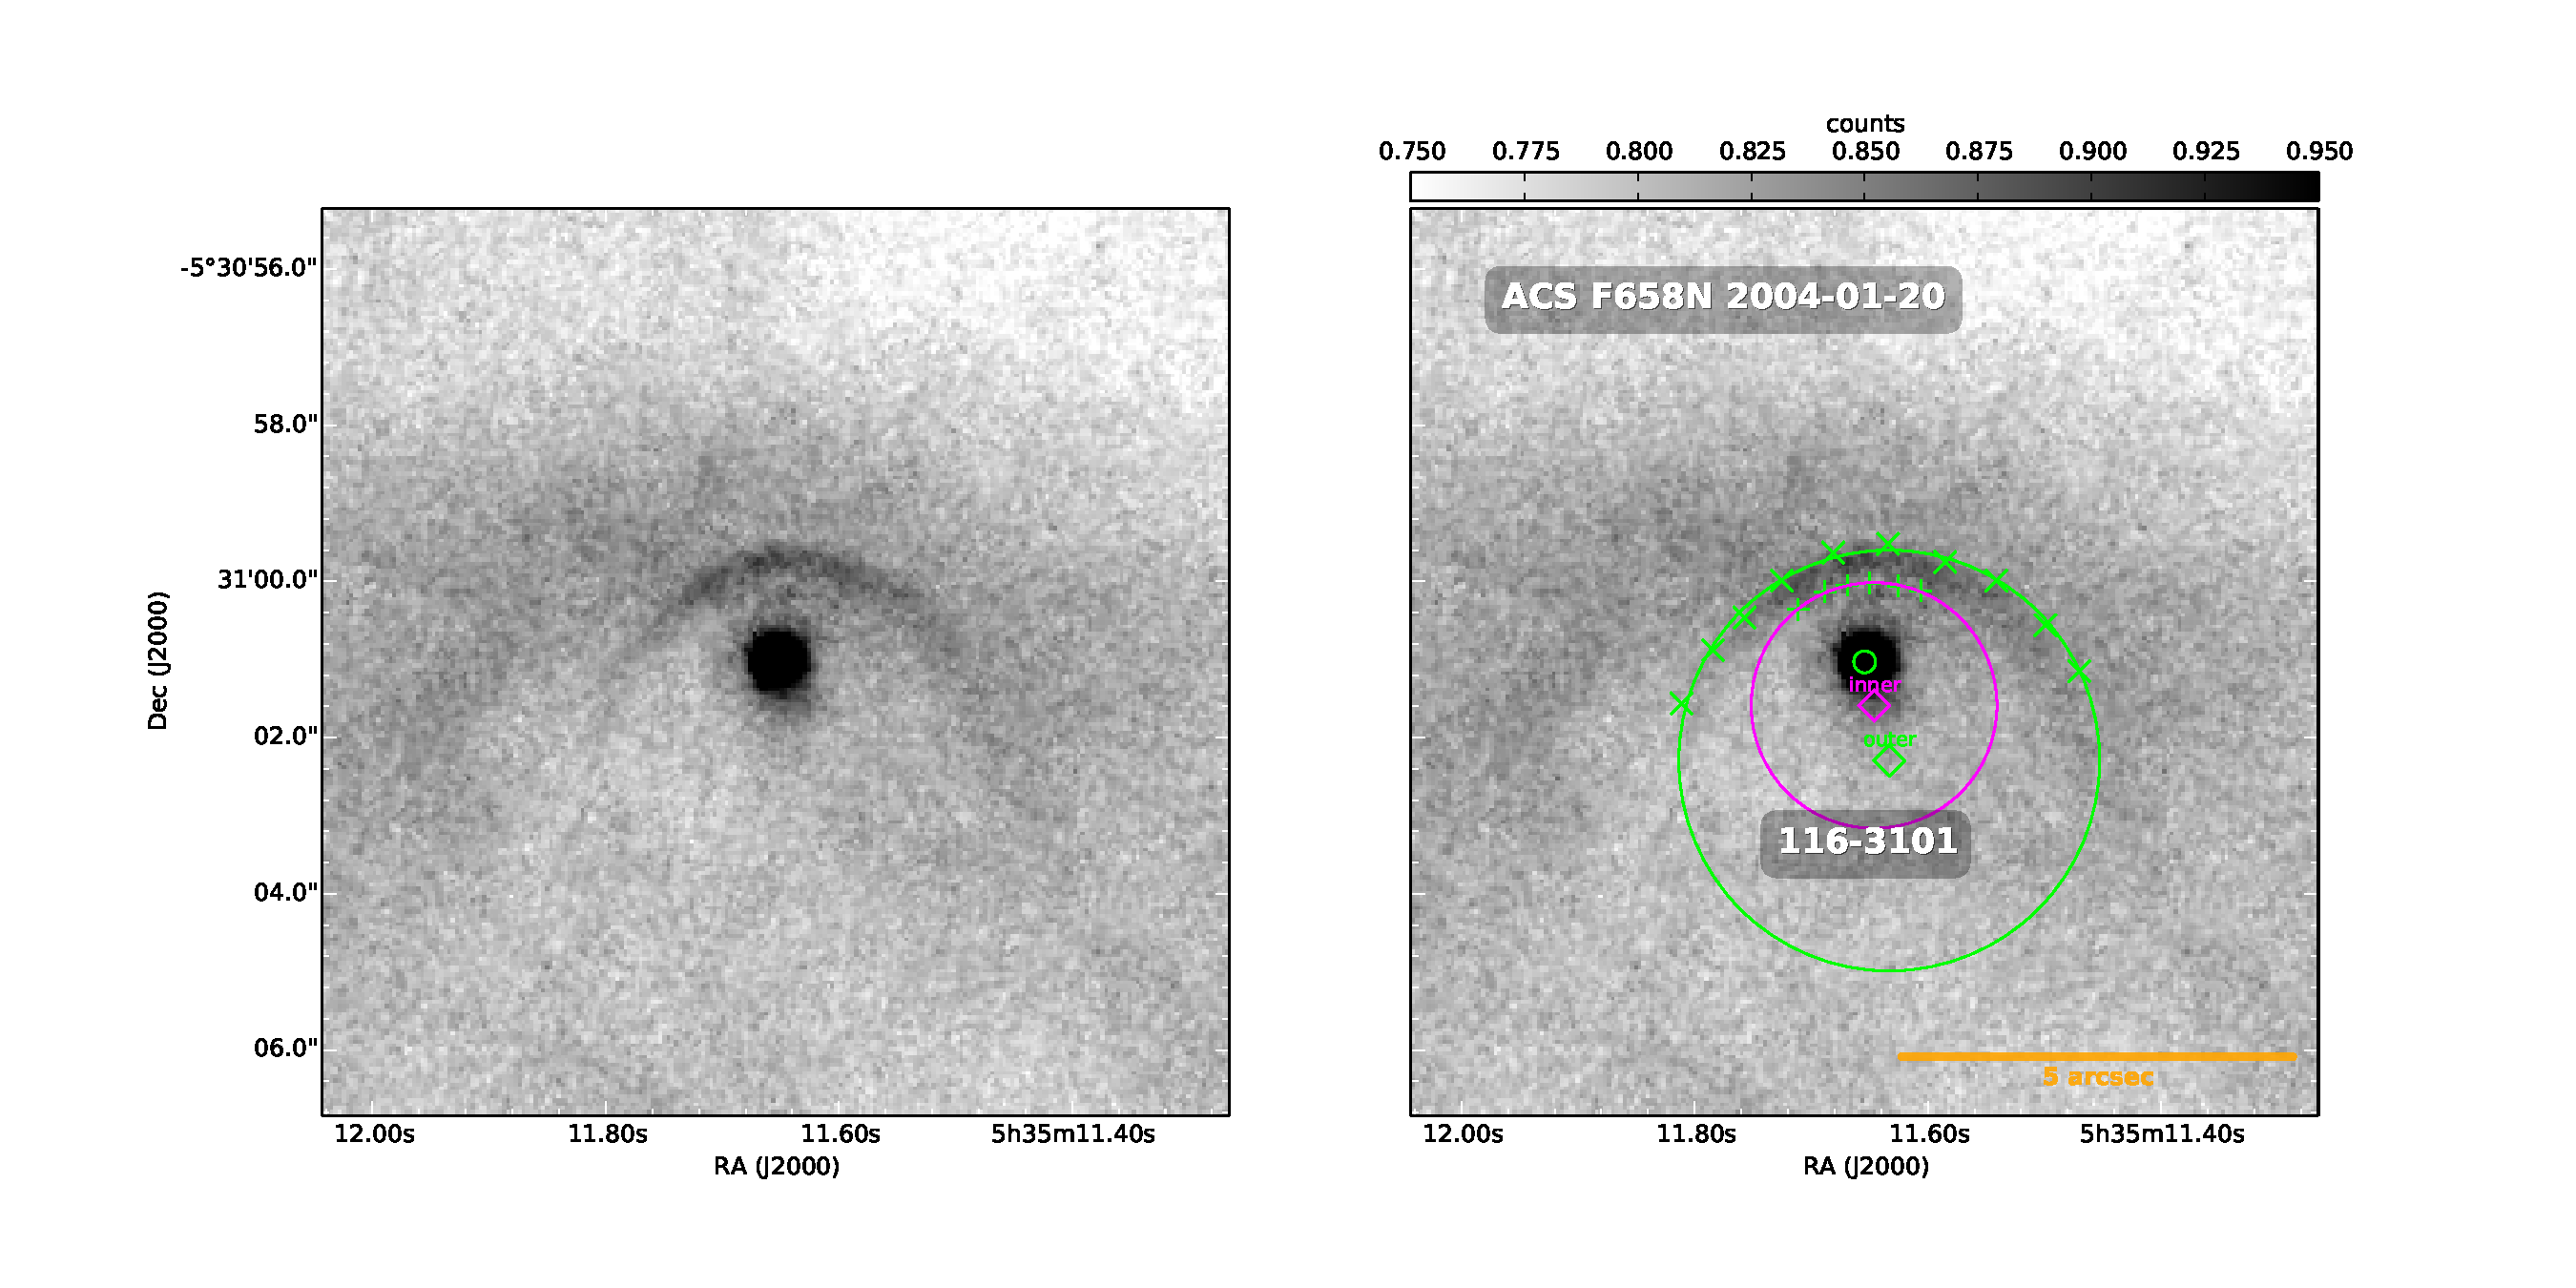
\includegraphics[width=\figwidth,  trim=60 50 100 50, clip]{j8oc14010_wcs/116-3101-Bally_14-images.pdf}}\\
   \framebox{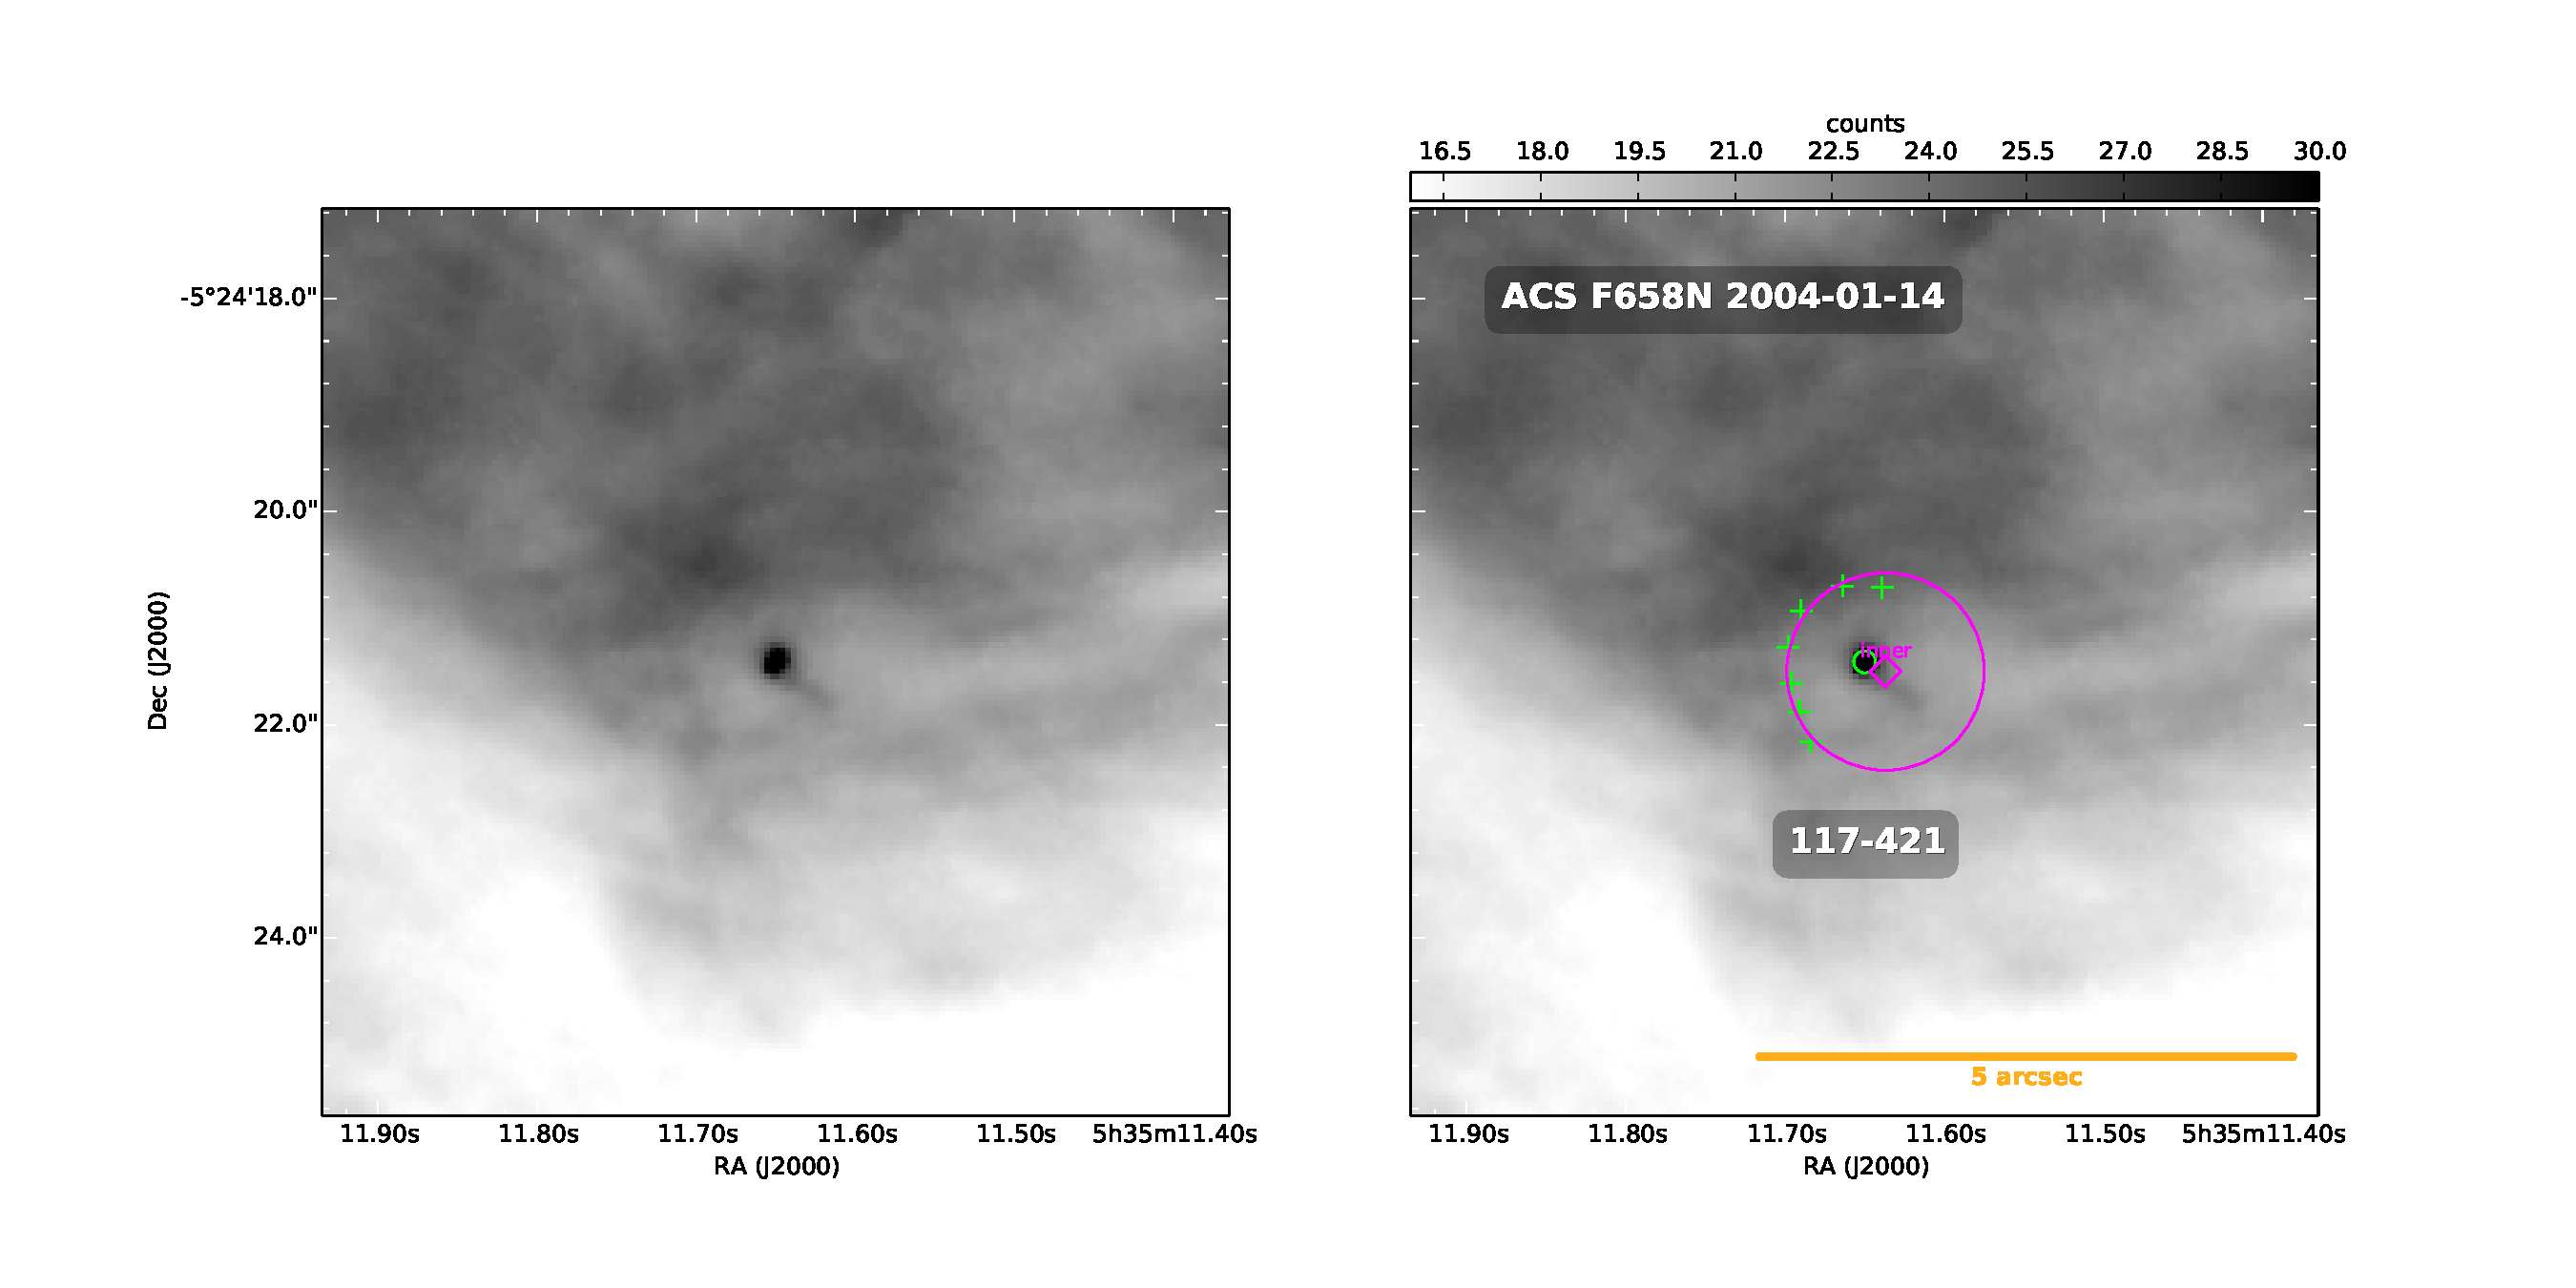
\includegraphics[width=\figwidth,  trim=60 50 100 50, clip]{j8oc01010_wcs/117-421-Bally_01-images.pdf}}
   &\framebox{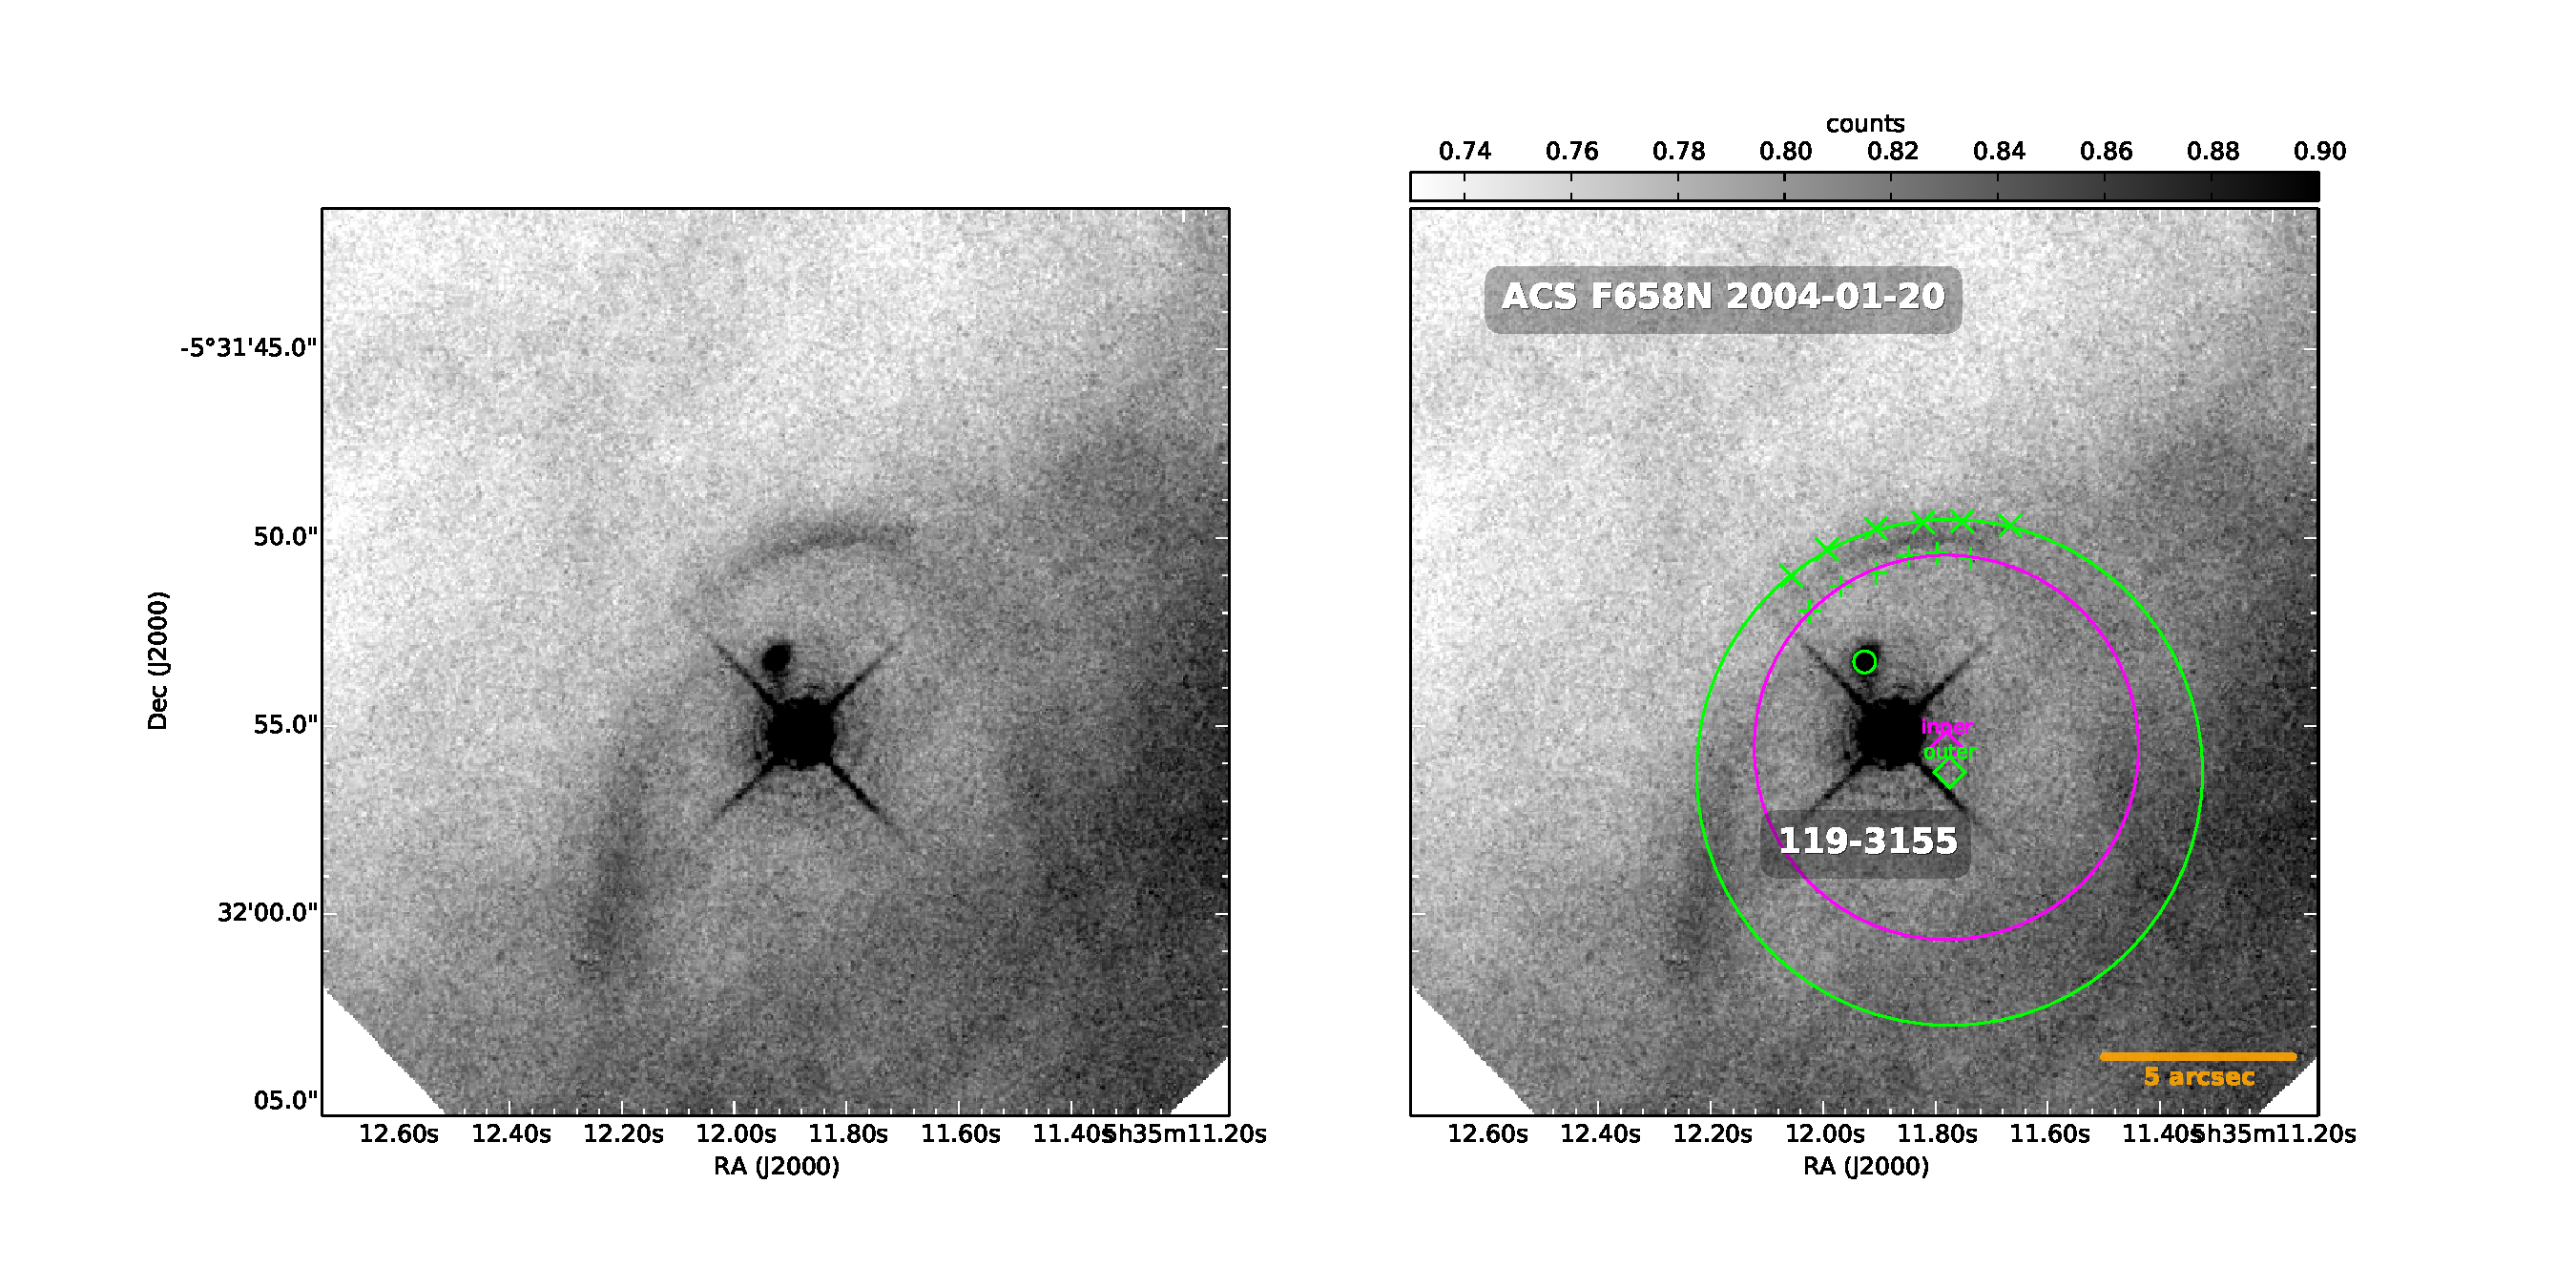
\includegraphics[width=\figwidth,  trim=60 50 100 50, clip]{j8oc14010_wcs/119-3155-Bally_14-images.pdf}}\\
   \framebox{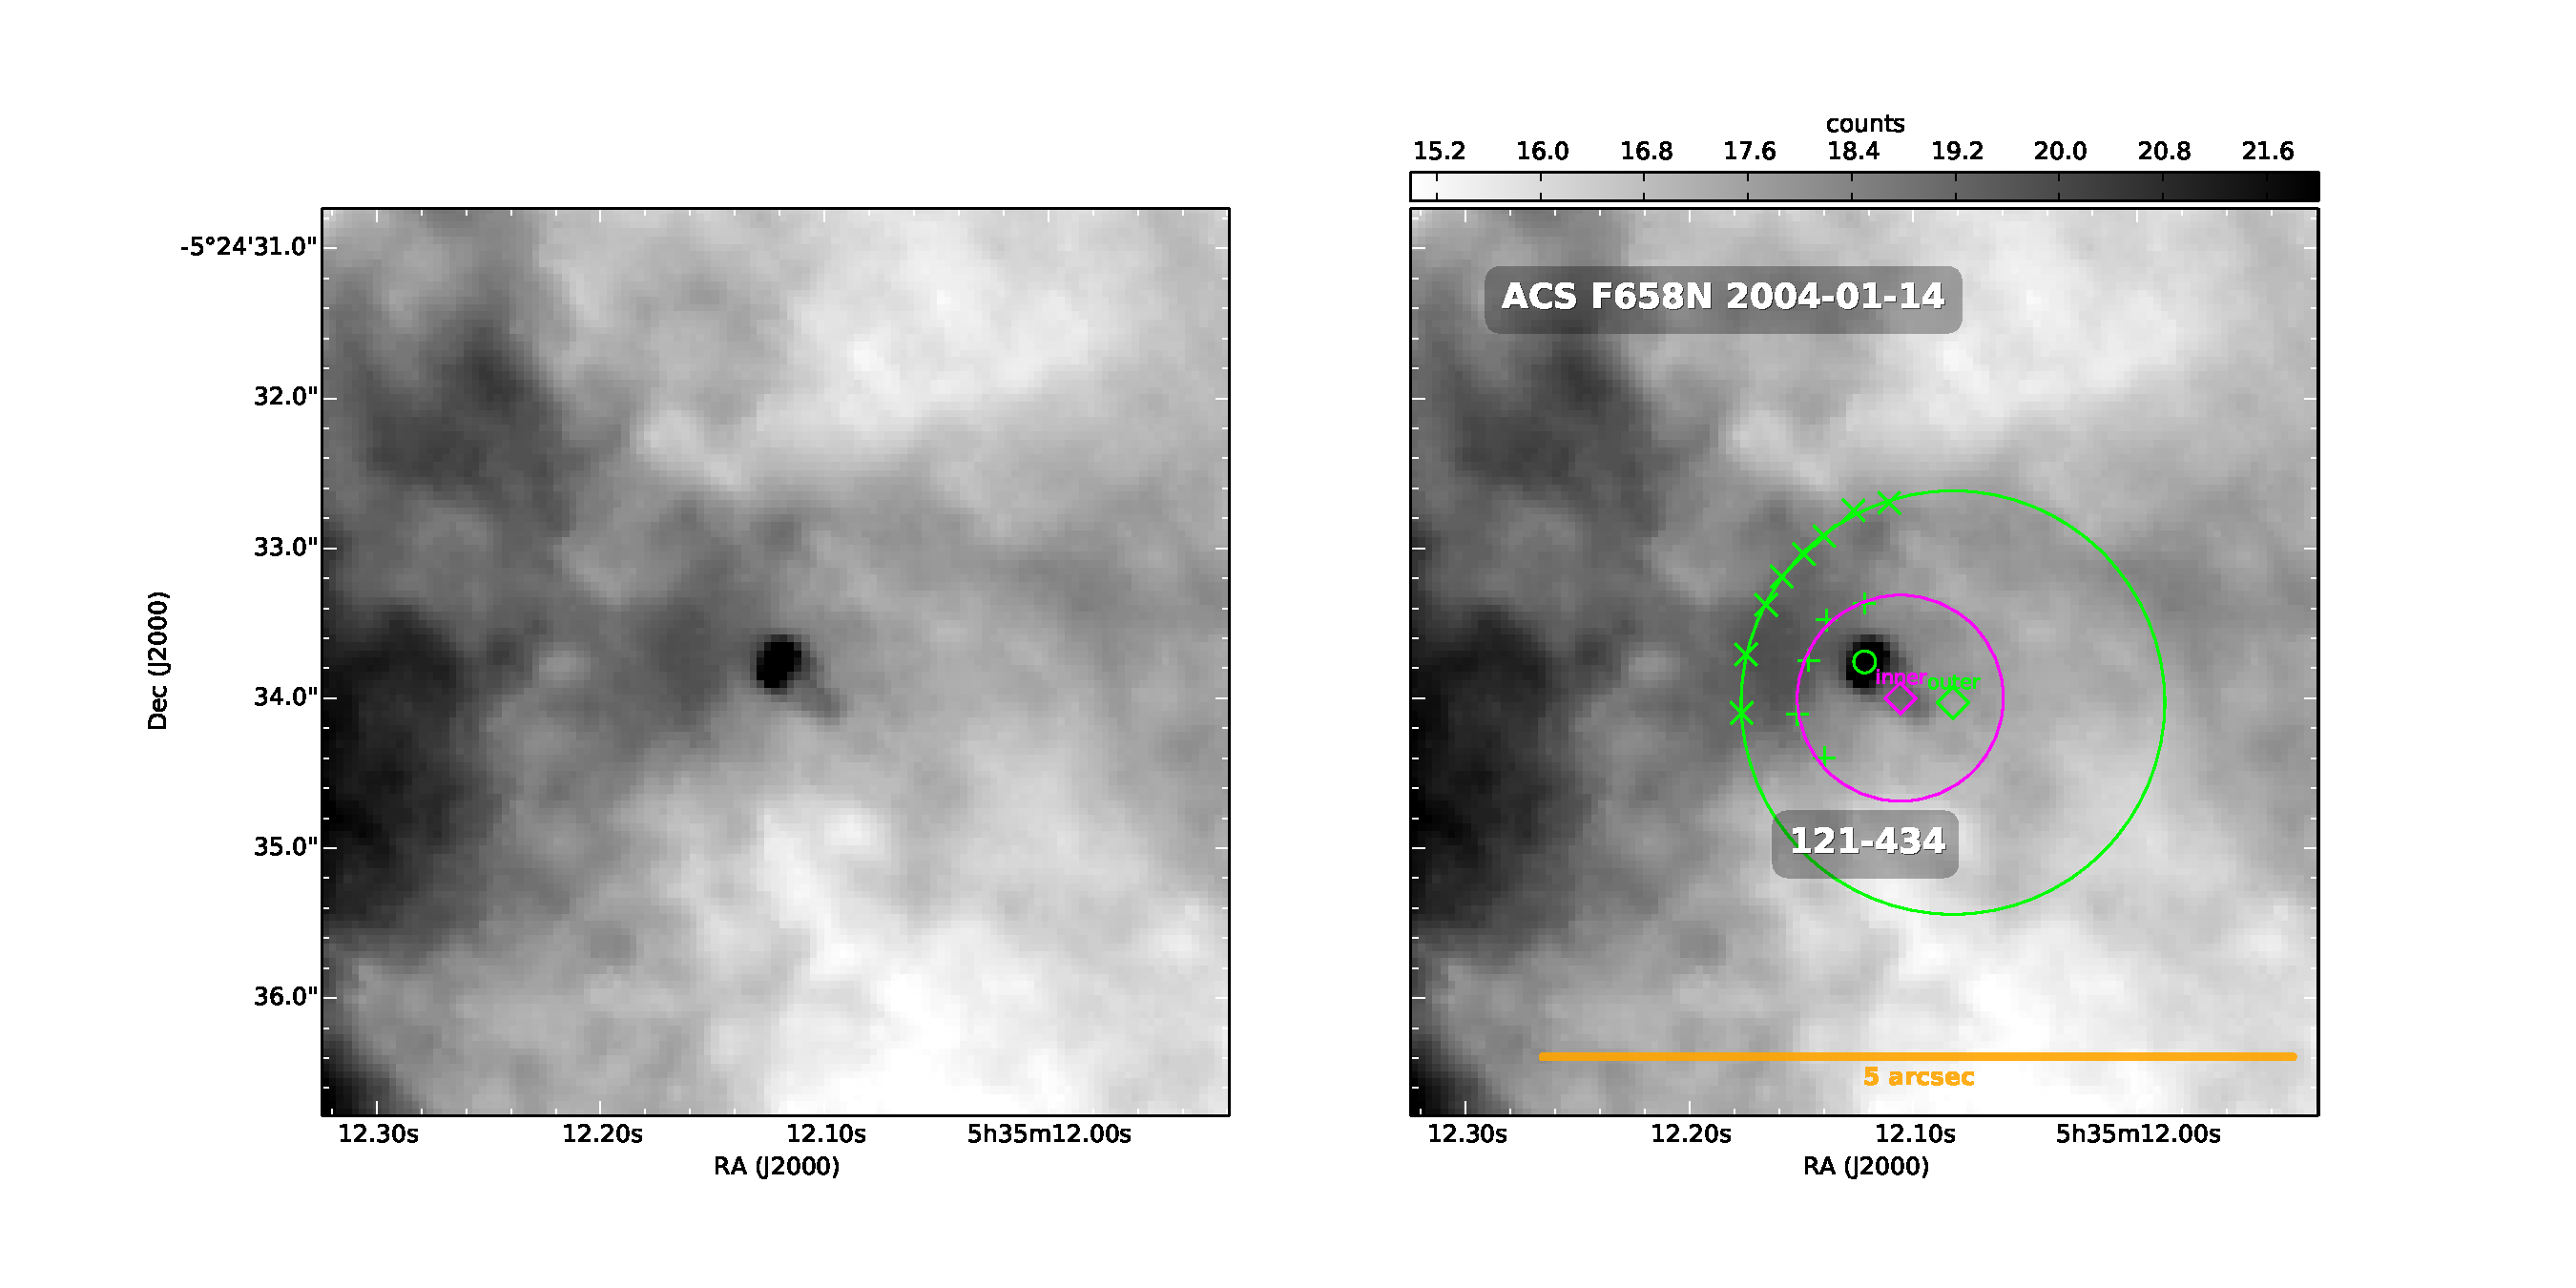
\includegraphics[width=\figwidth,  trim=60 50 100 50, clip]{j8oc01010_wcs/121-434-Bally_01-images.pdf}}
%   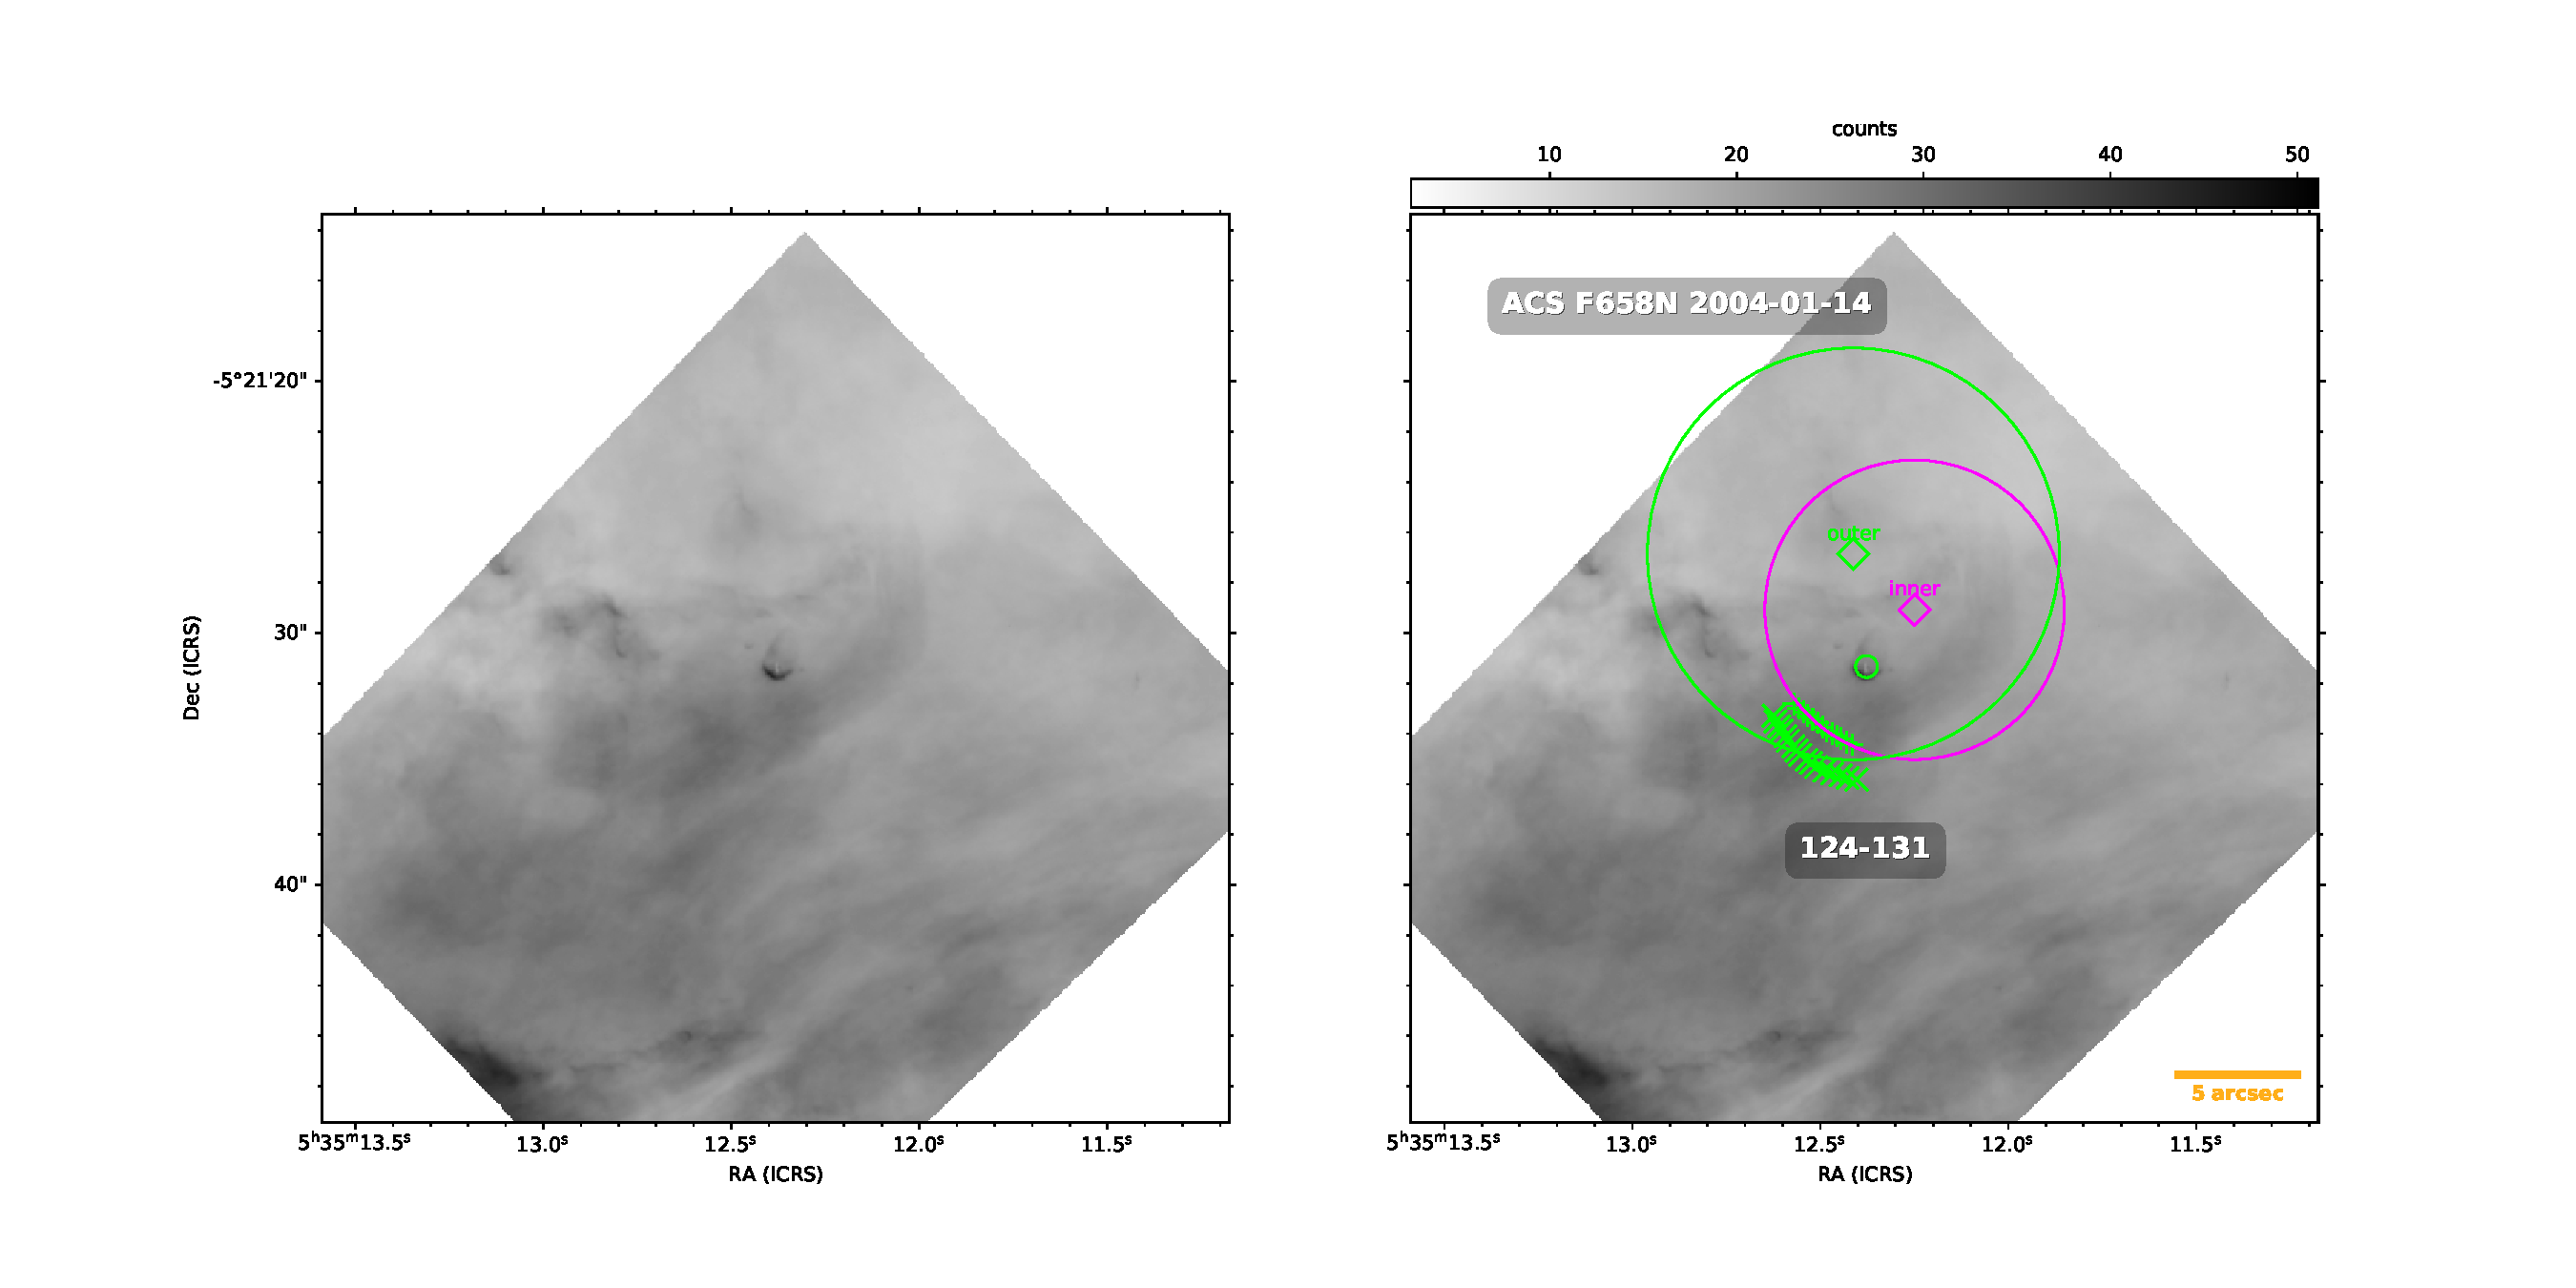
\includegraphics[width=0.47\linewidth,  trim=60 50 100 50, clip]{j8oc01010_wcs/124-131-Bally_01-images.pdf}
   &\framebox{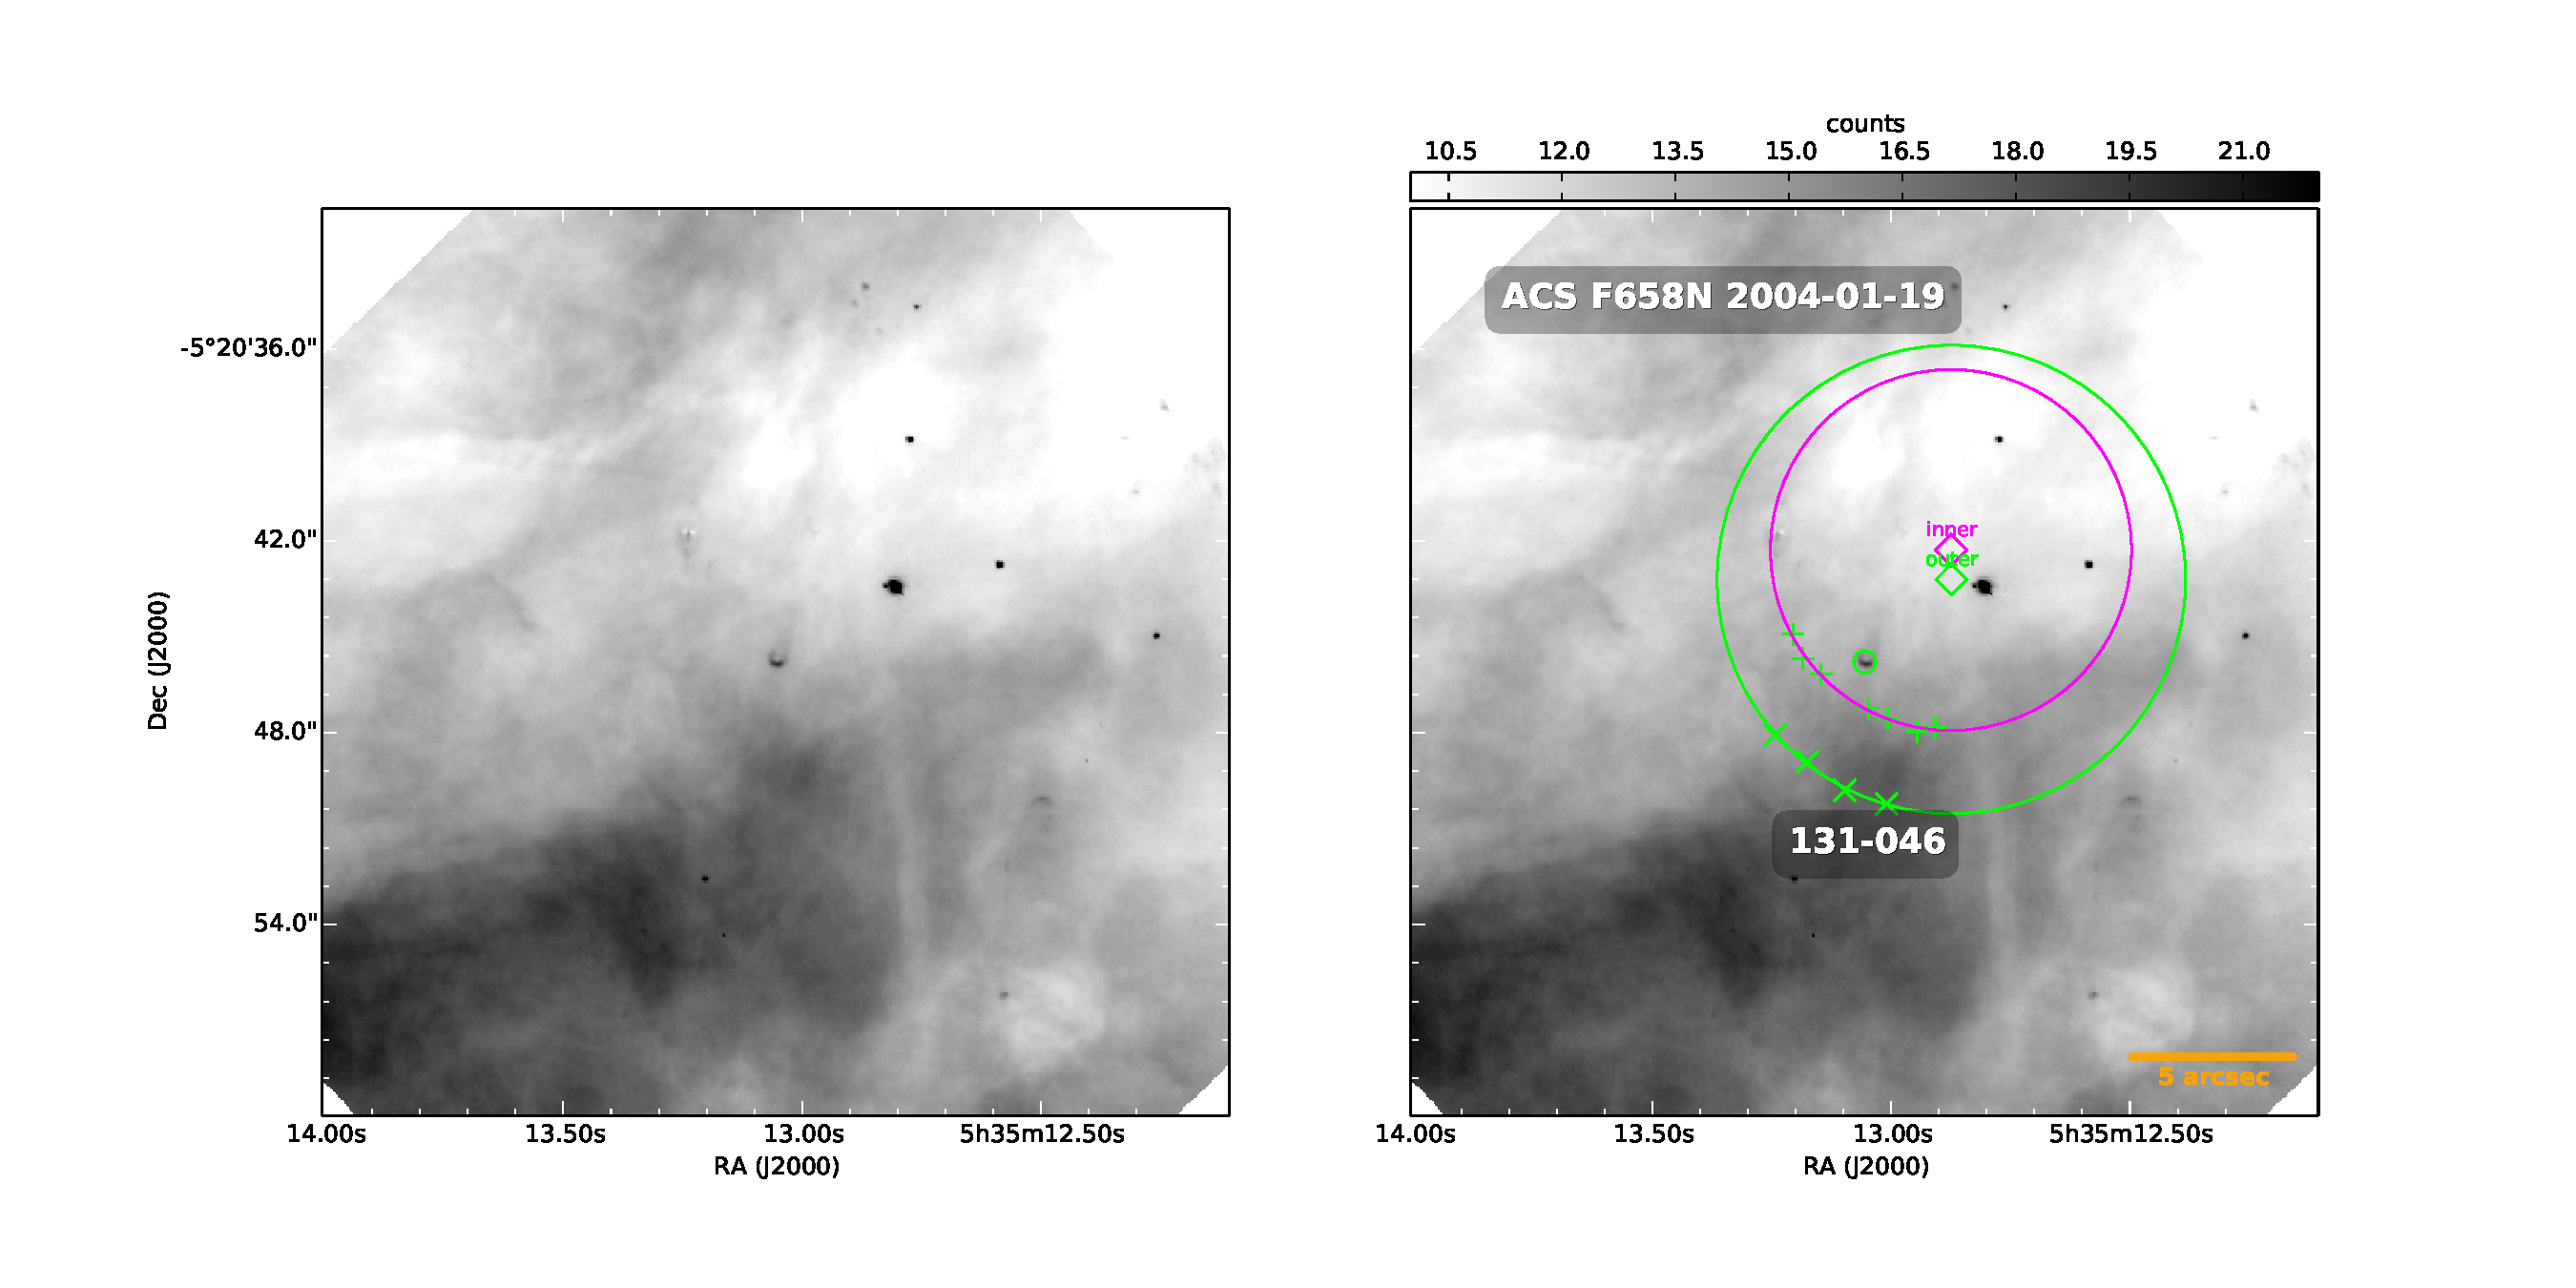
\includegraphics[width=\figwidth,  trim=60 50 100 50, clip]{j8oc02010_wcs/131-046-Bally_02-images.pdf}}\\
   \framebox{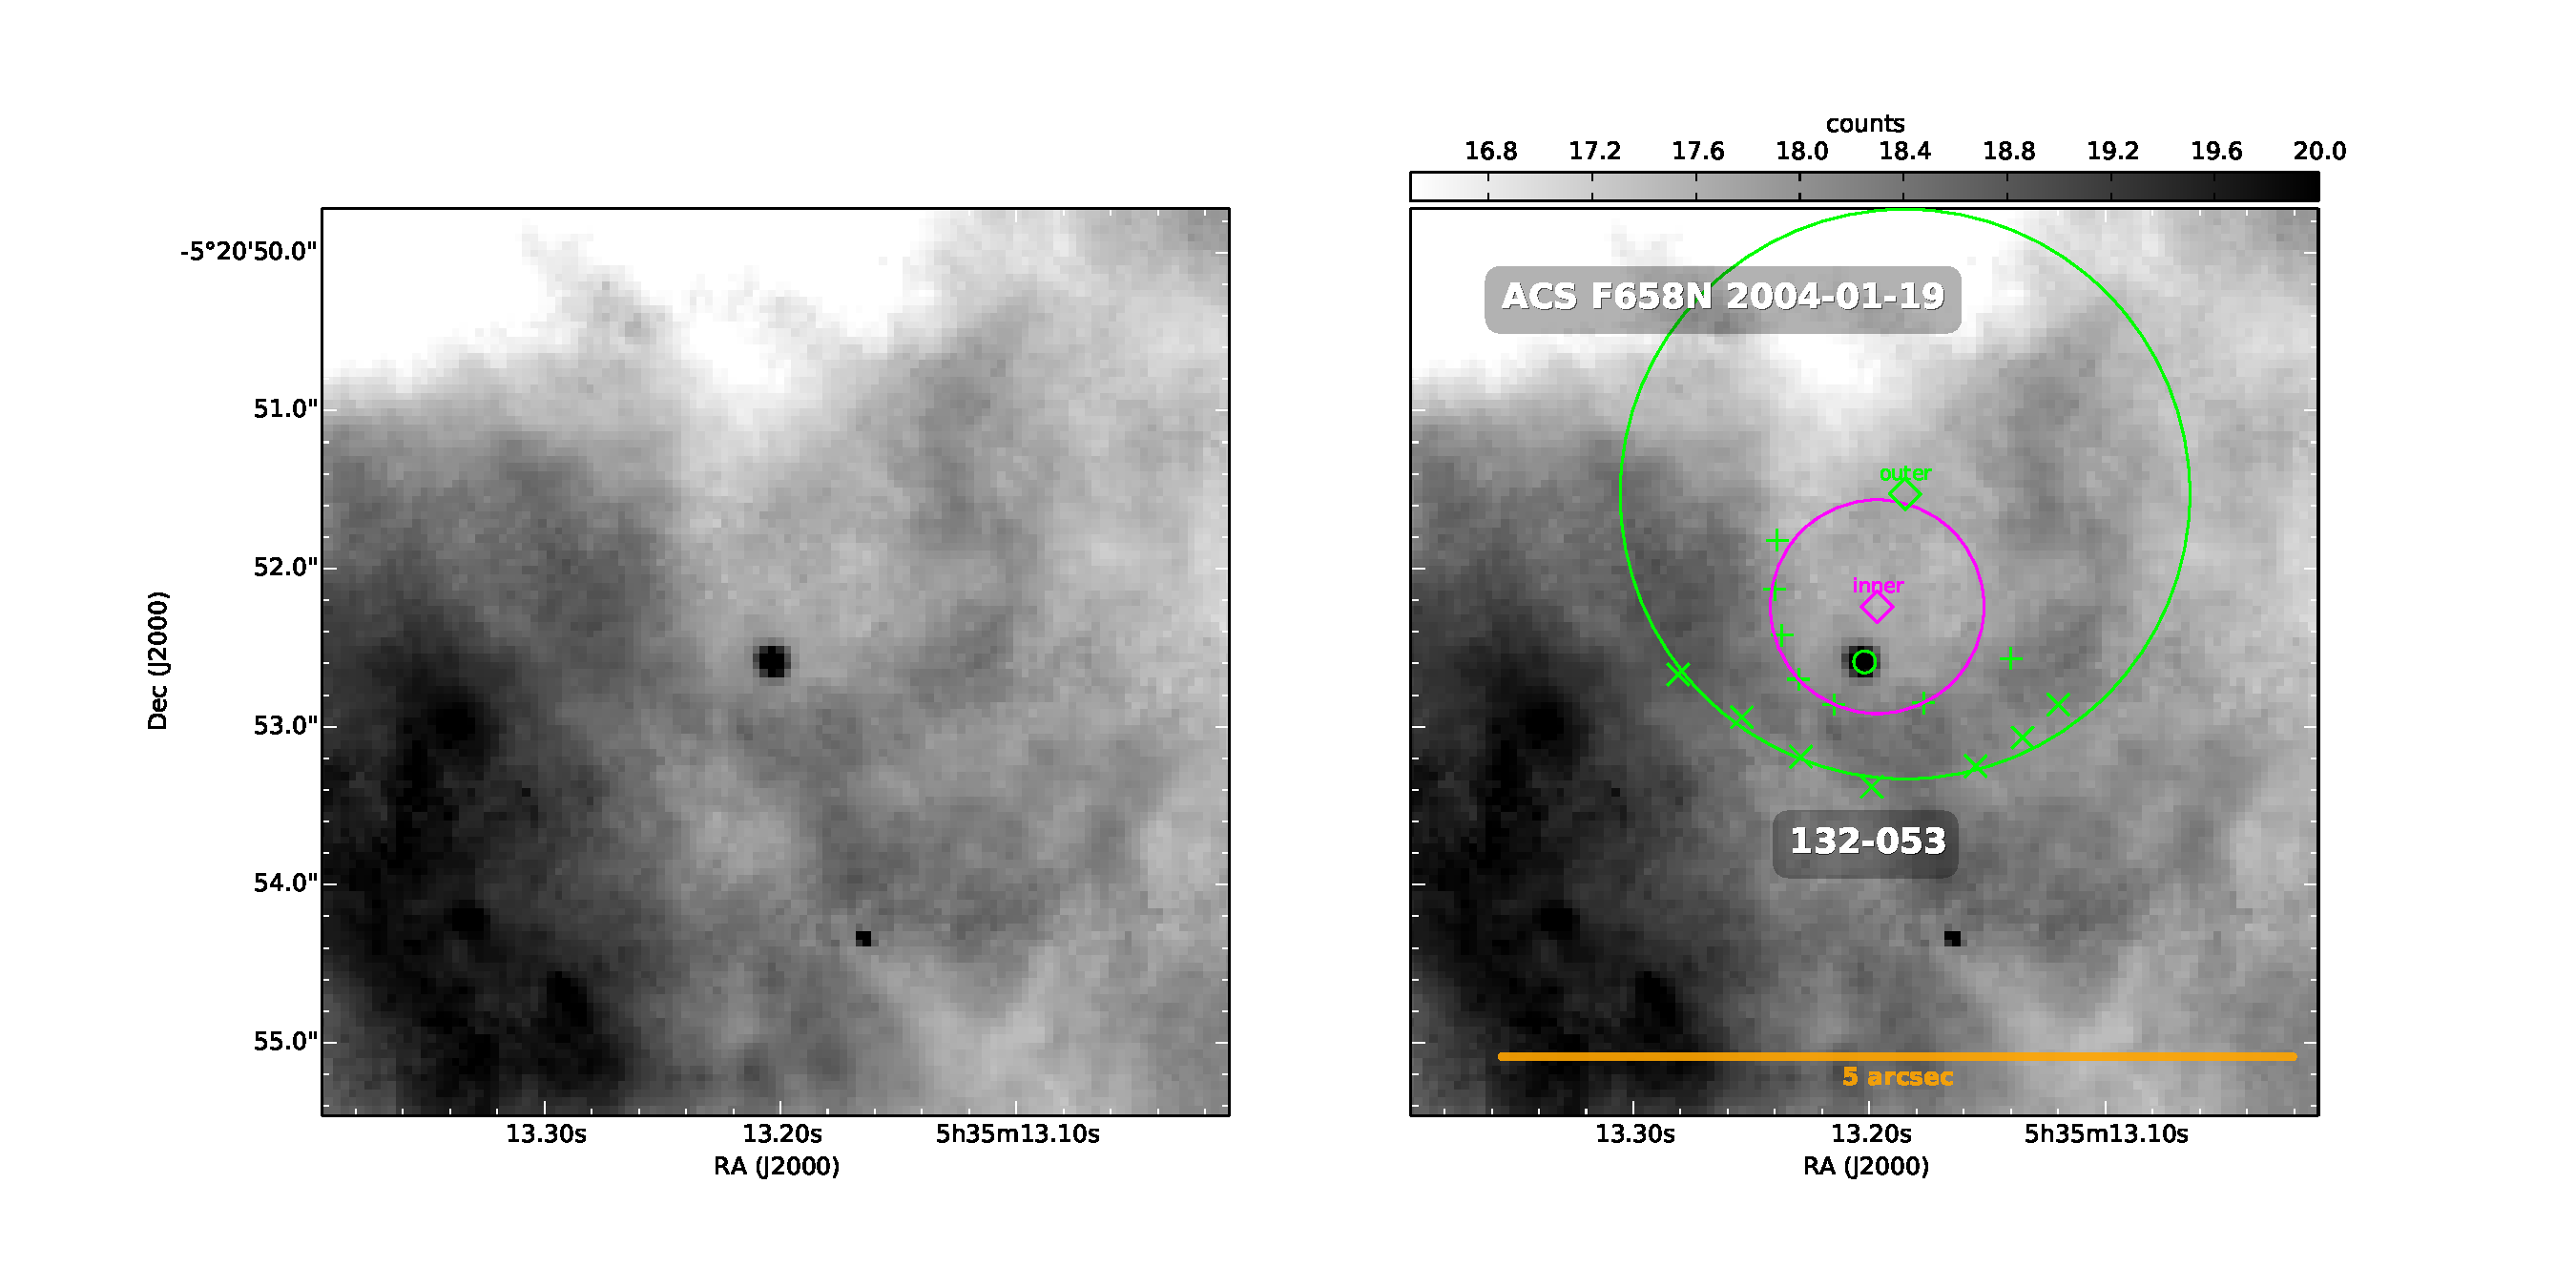
\includegraphics[width=\figwidth,  trim=60 50 100 50, clip]{j8oc02010_wcs/132-053-Bally_02-images.pdf}}
   & \framebox{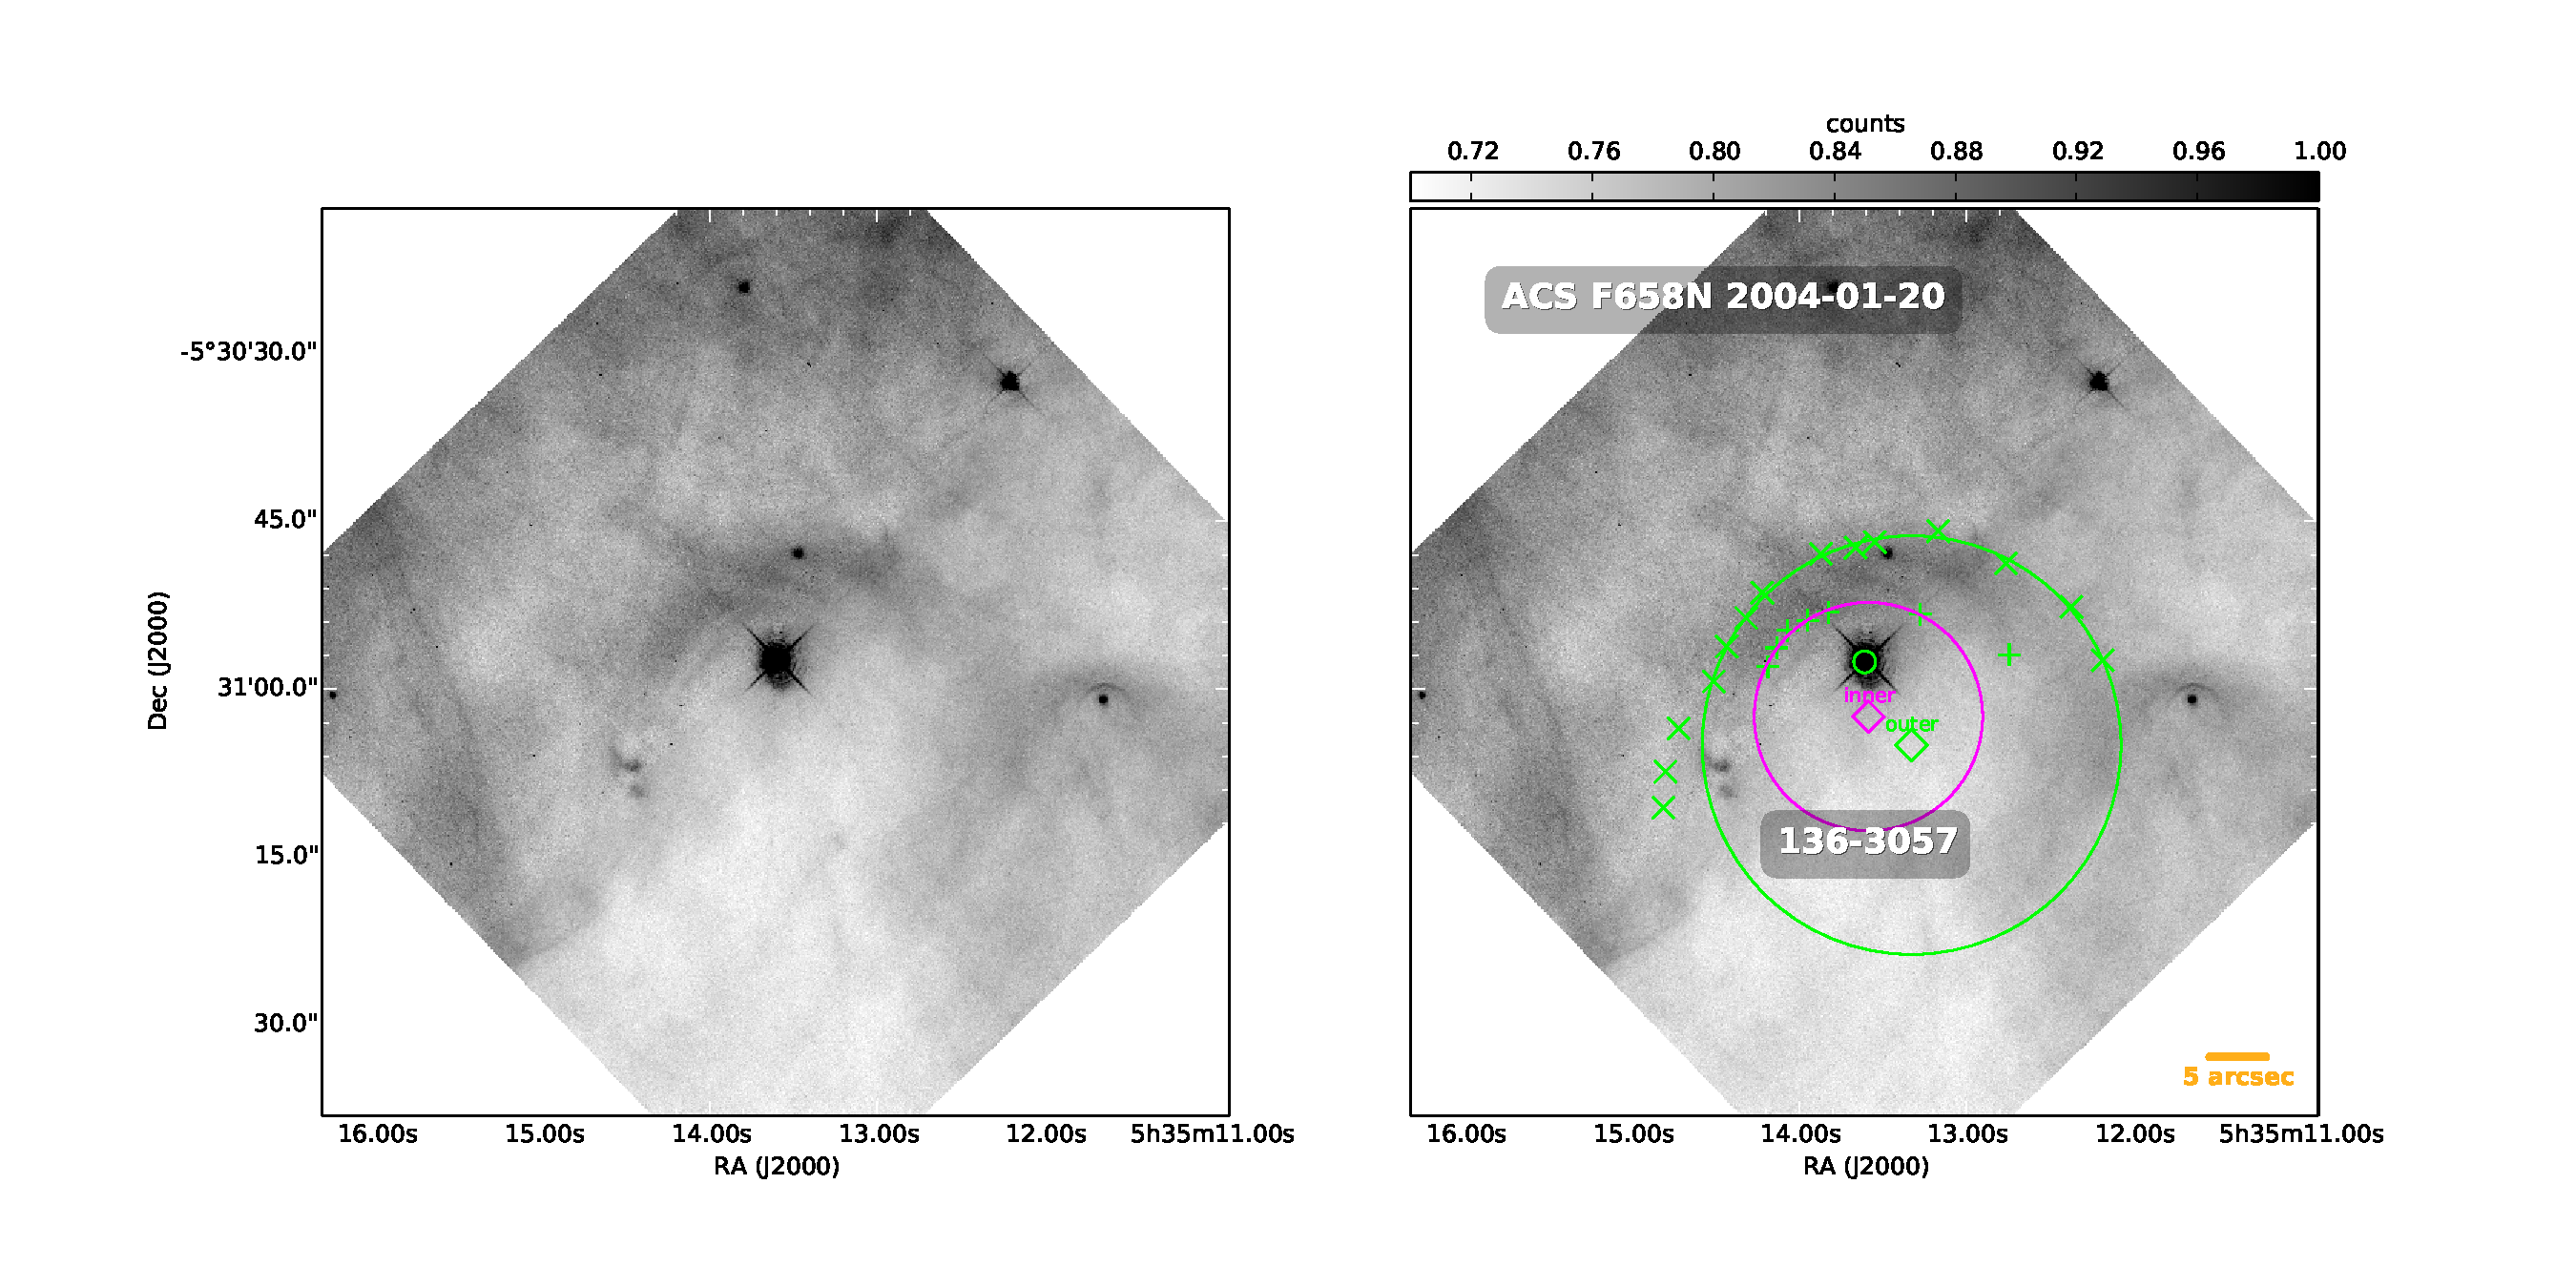
\includegraphics[width=\figwidth,  trim=60 50 100 50, clip]{j8oc14010_wcs/136-3057-Bally_14-images.pdf}}\\
\end{tabular}
\end{figure*}   

\begin{figure*}
\setlength\tabcolsep{1.5pt}
\begin{tabular}{l l}
 \framebox{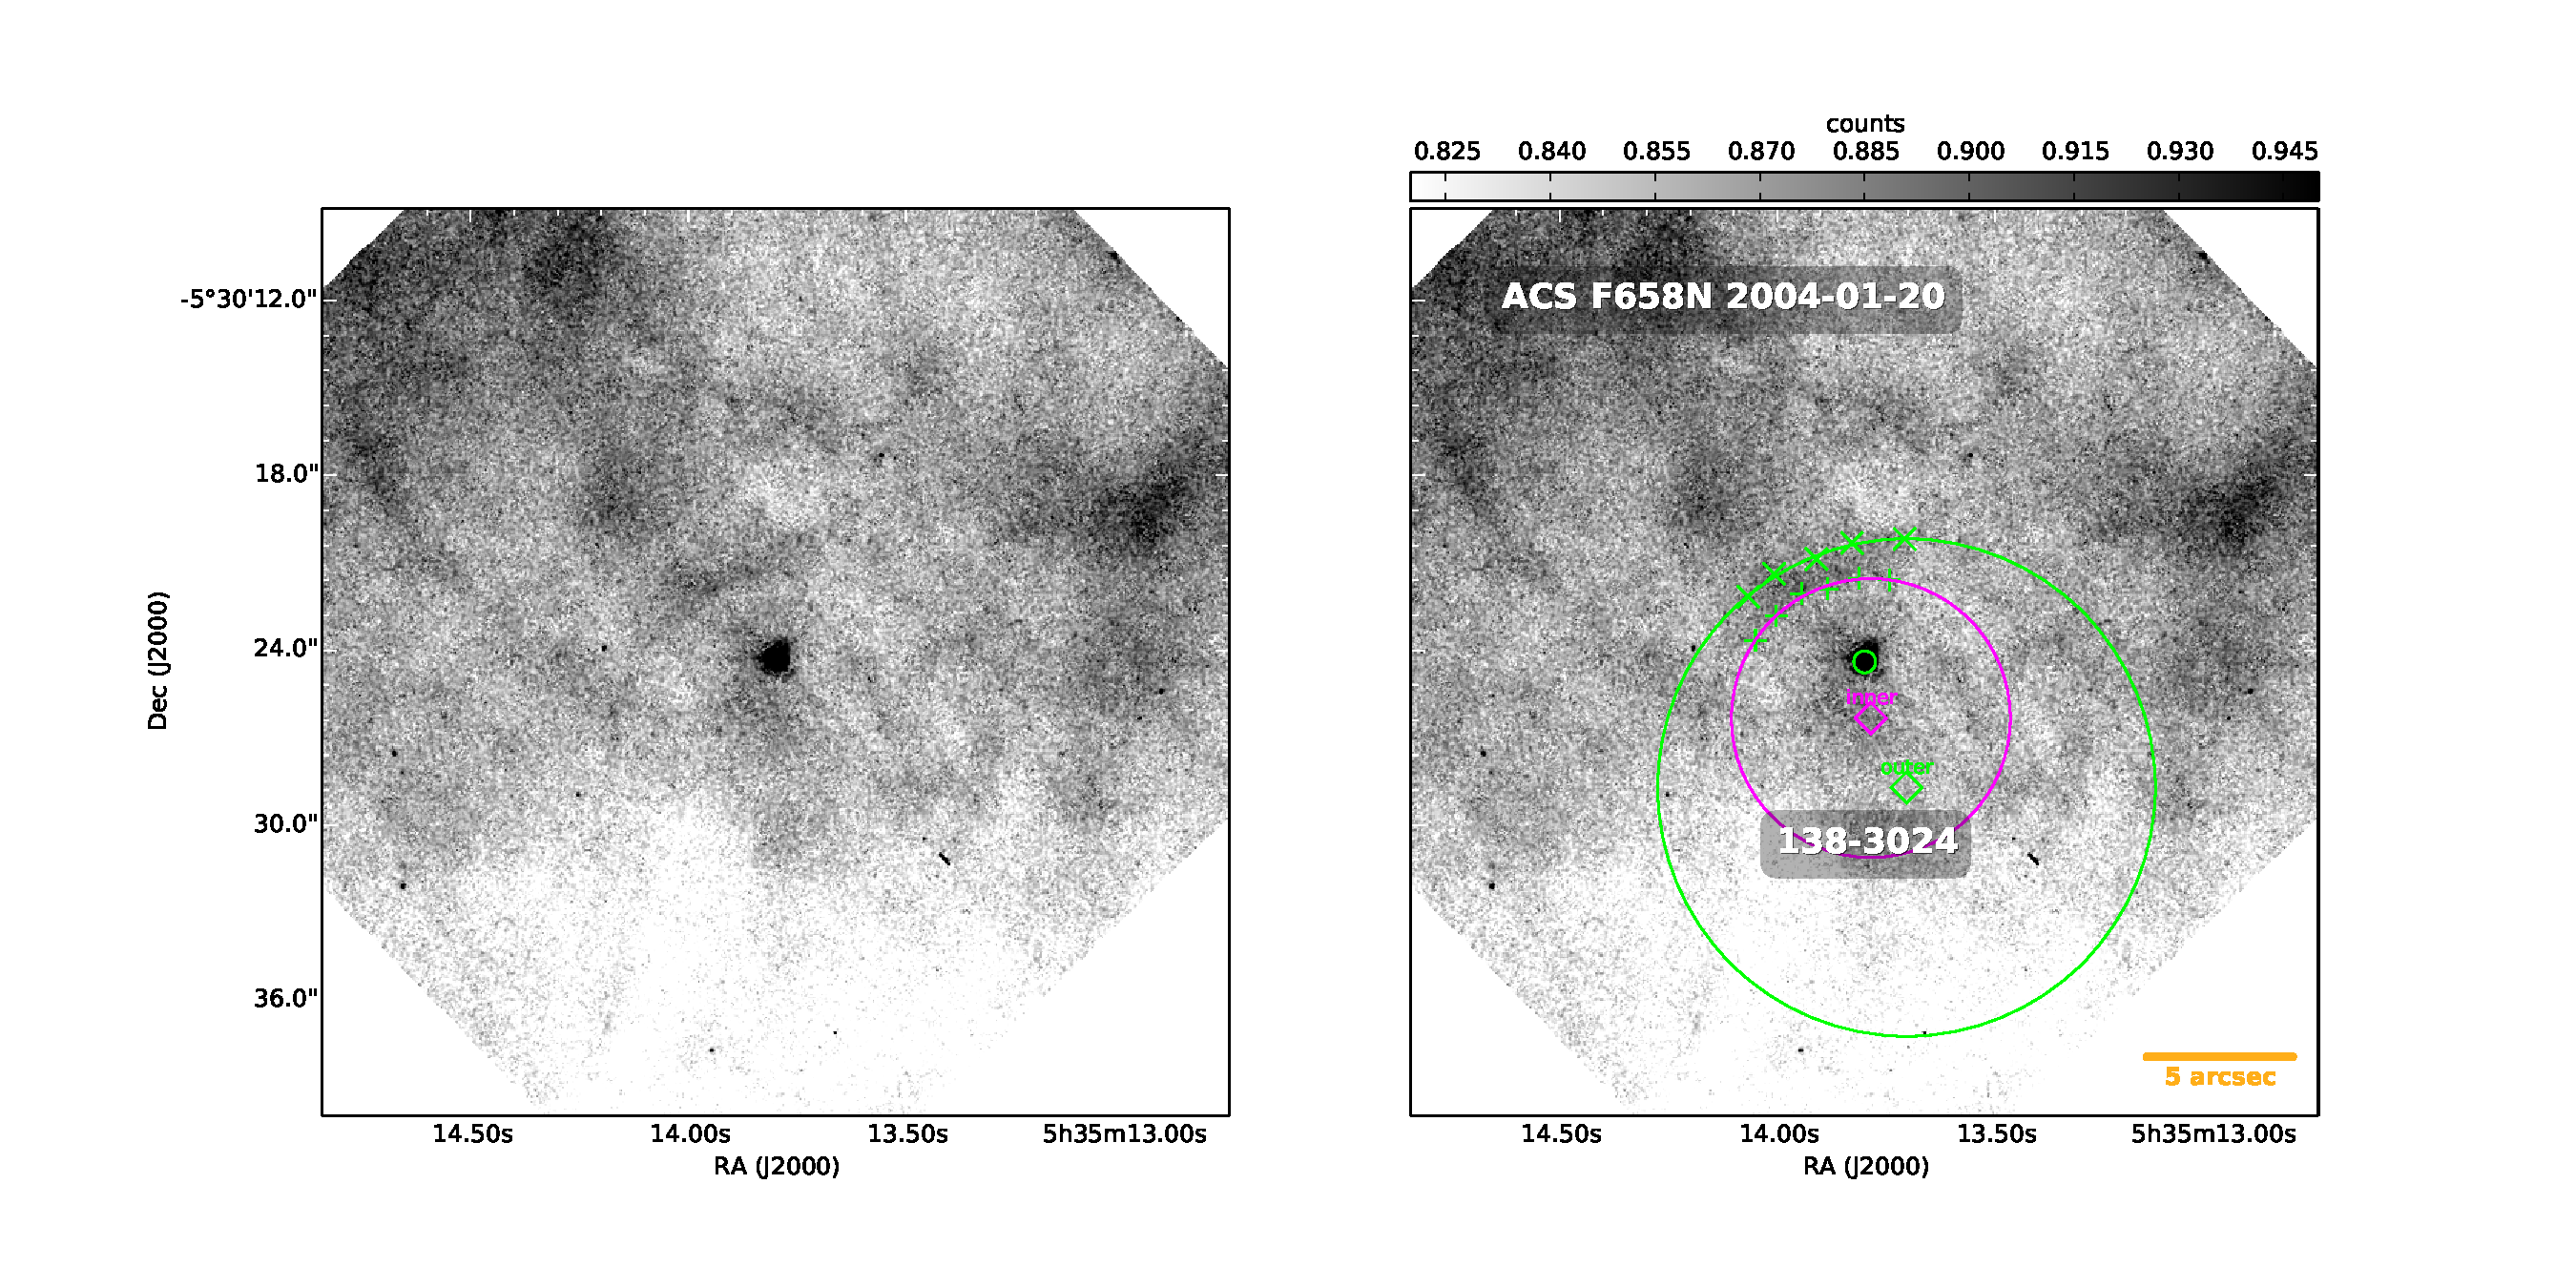
\includegraphics[width=\figwidth,  trim=60 50 100 50, clip]{j8oc14010_wcs/138-3024-Bally_14-images.pdf}}
   &\framebox{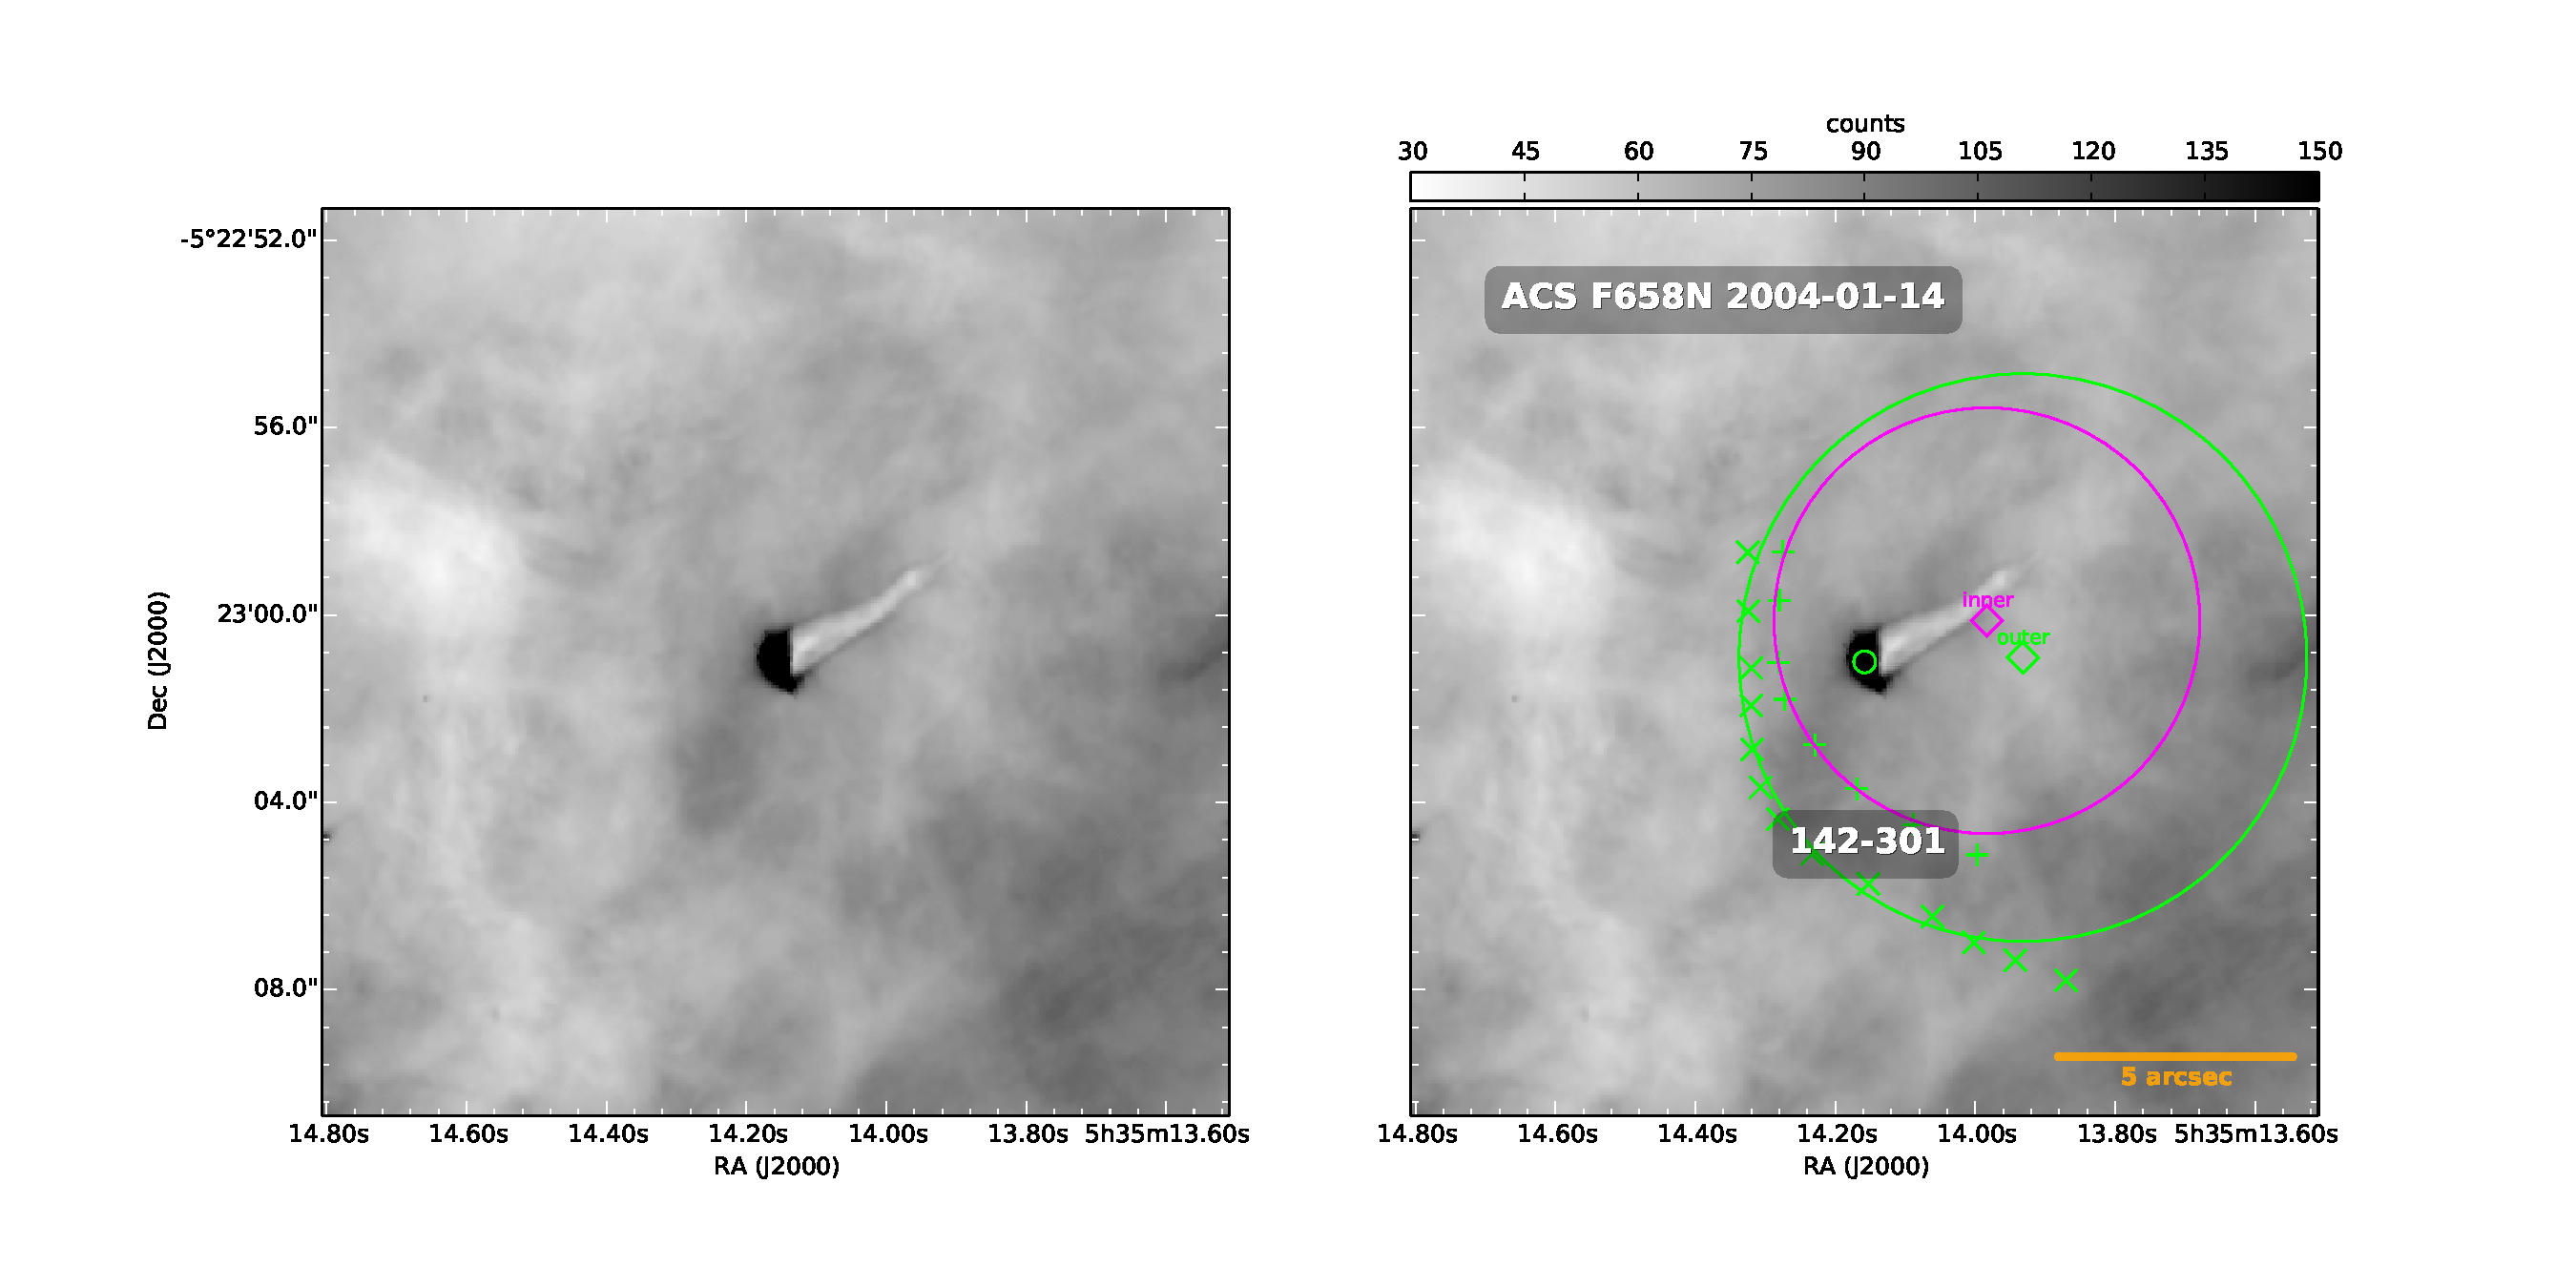
\includegraphics[width=\figwidth,  trim=60 50 100 50, clip]{j8oc01010_wcs/142-301-Bally_01-images.pdf}}\\
   \framebox{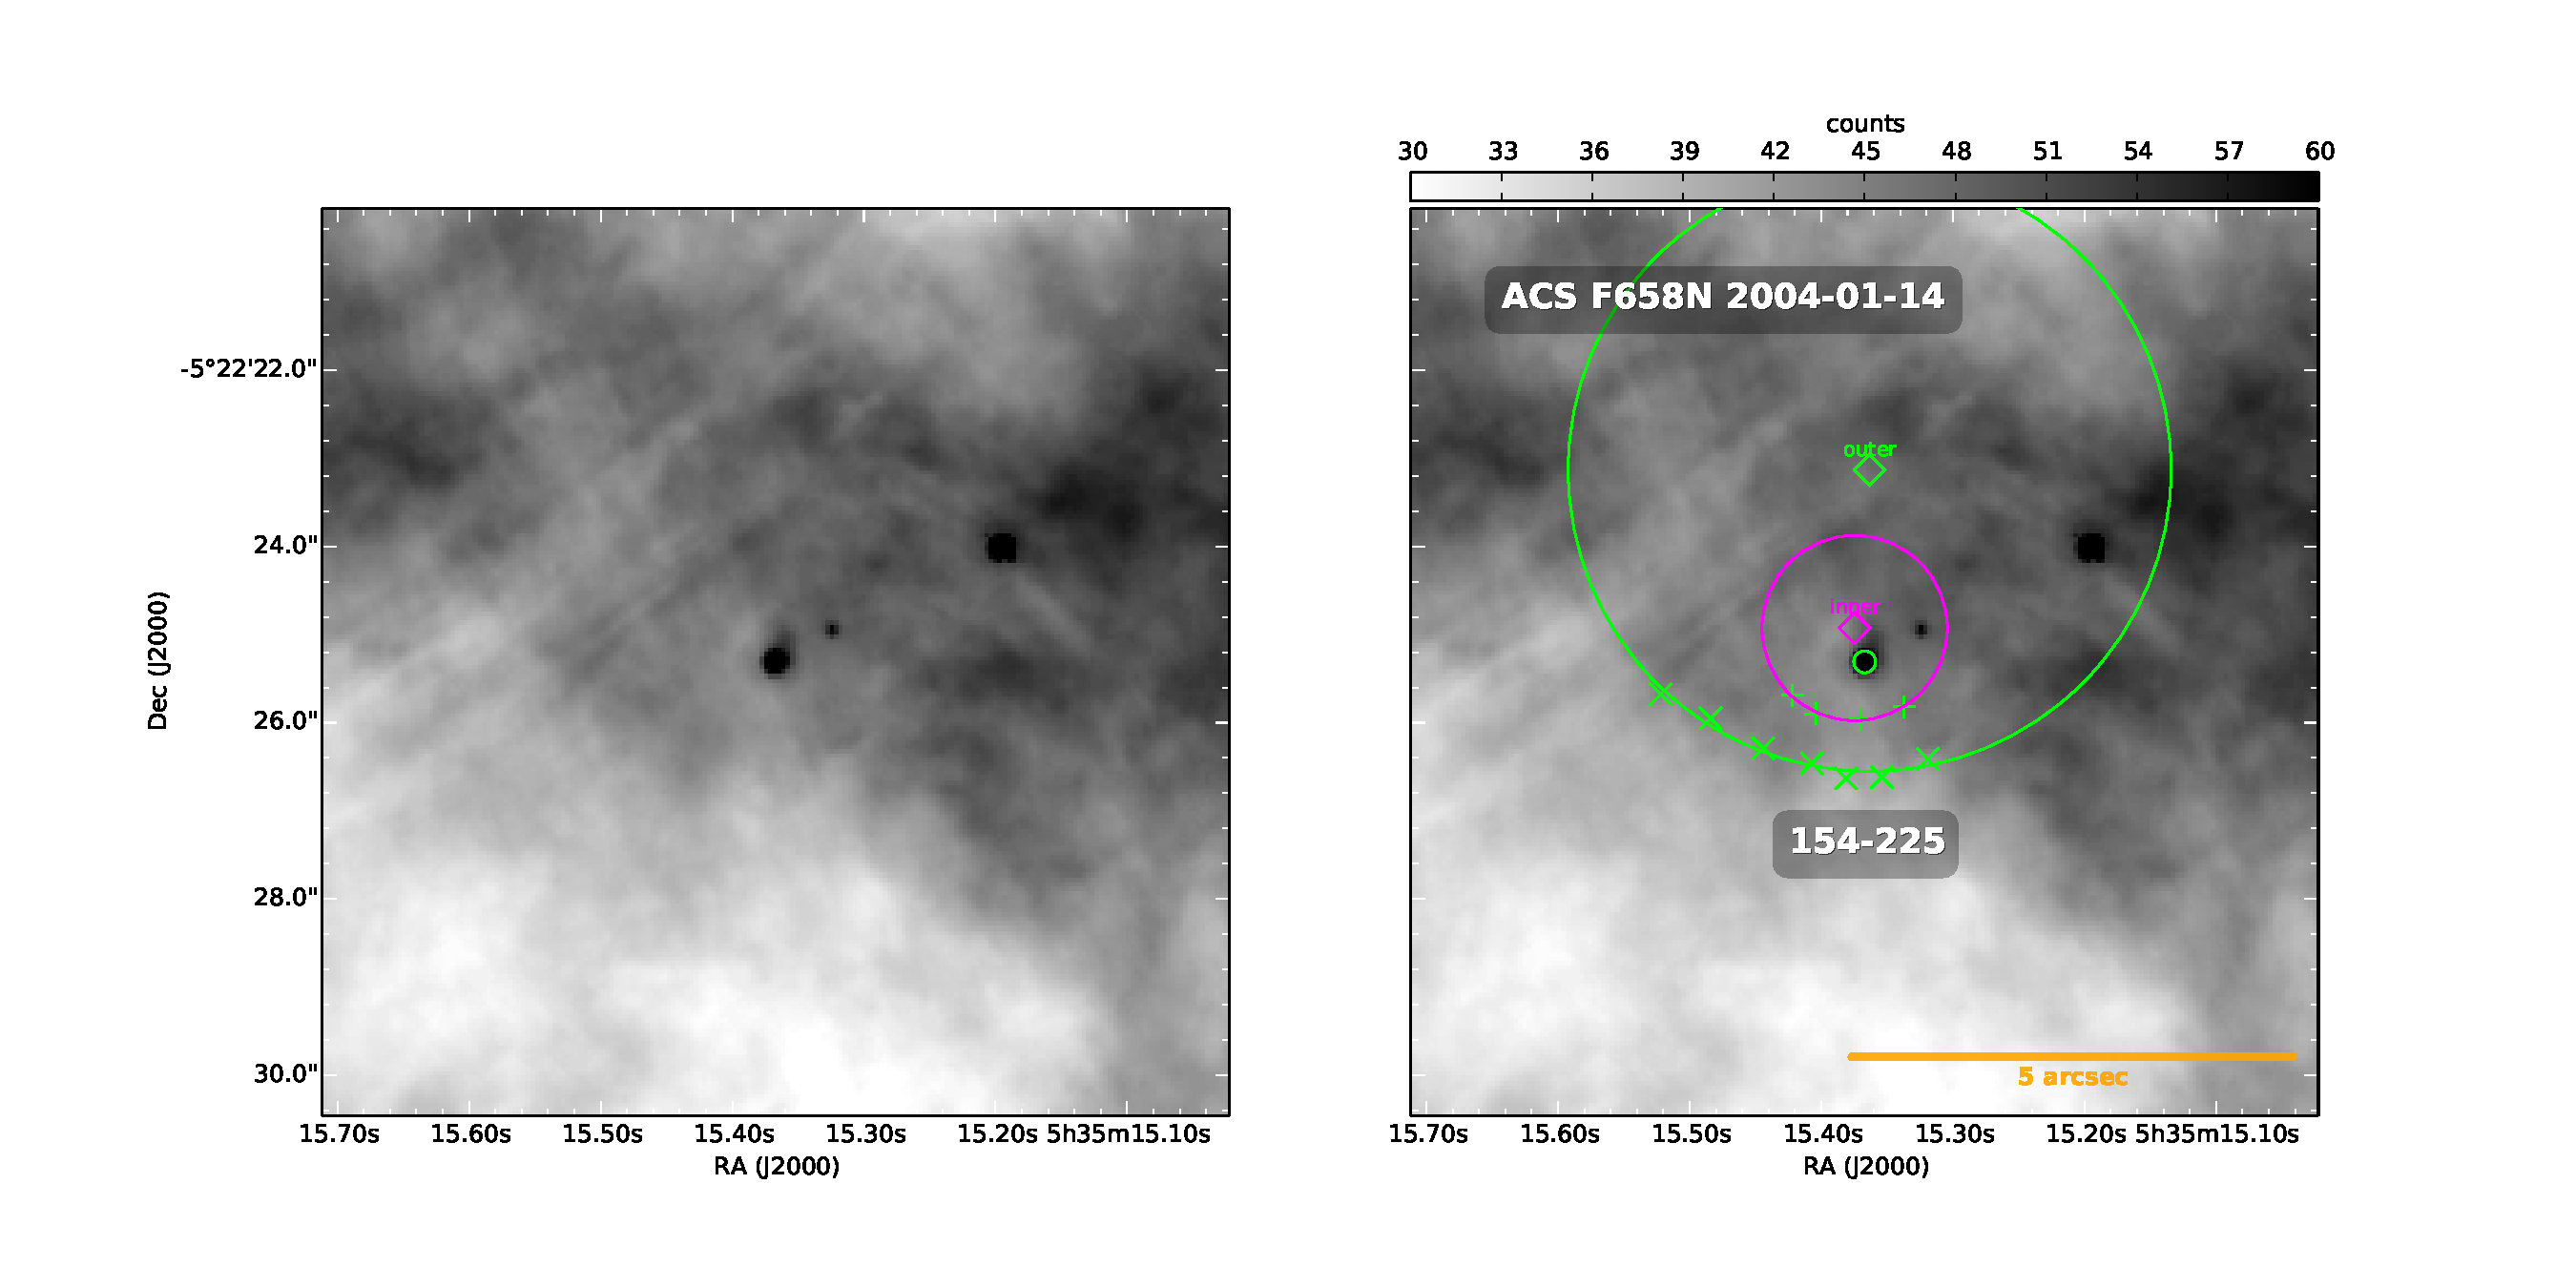
\includegraphics[width=\figwidth,  trim=60 50 100 50, clip]{j8oc01010_wcs/154-225-Bally_01-images.pdf}}
    &\framebox{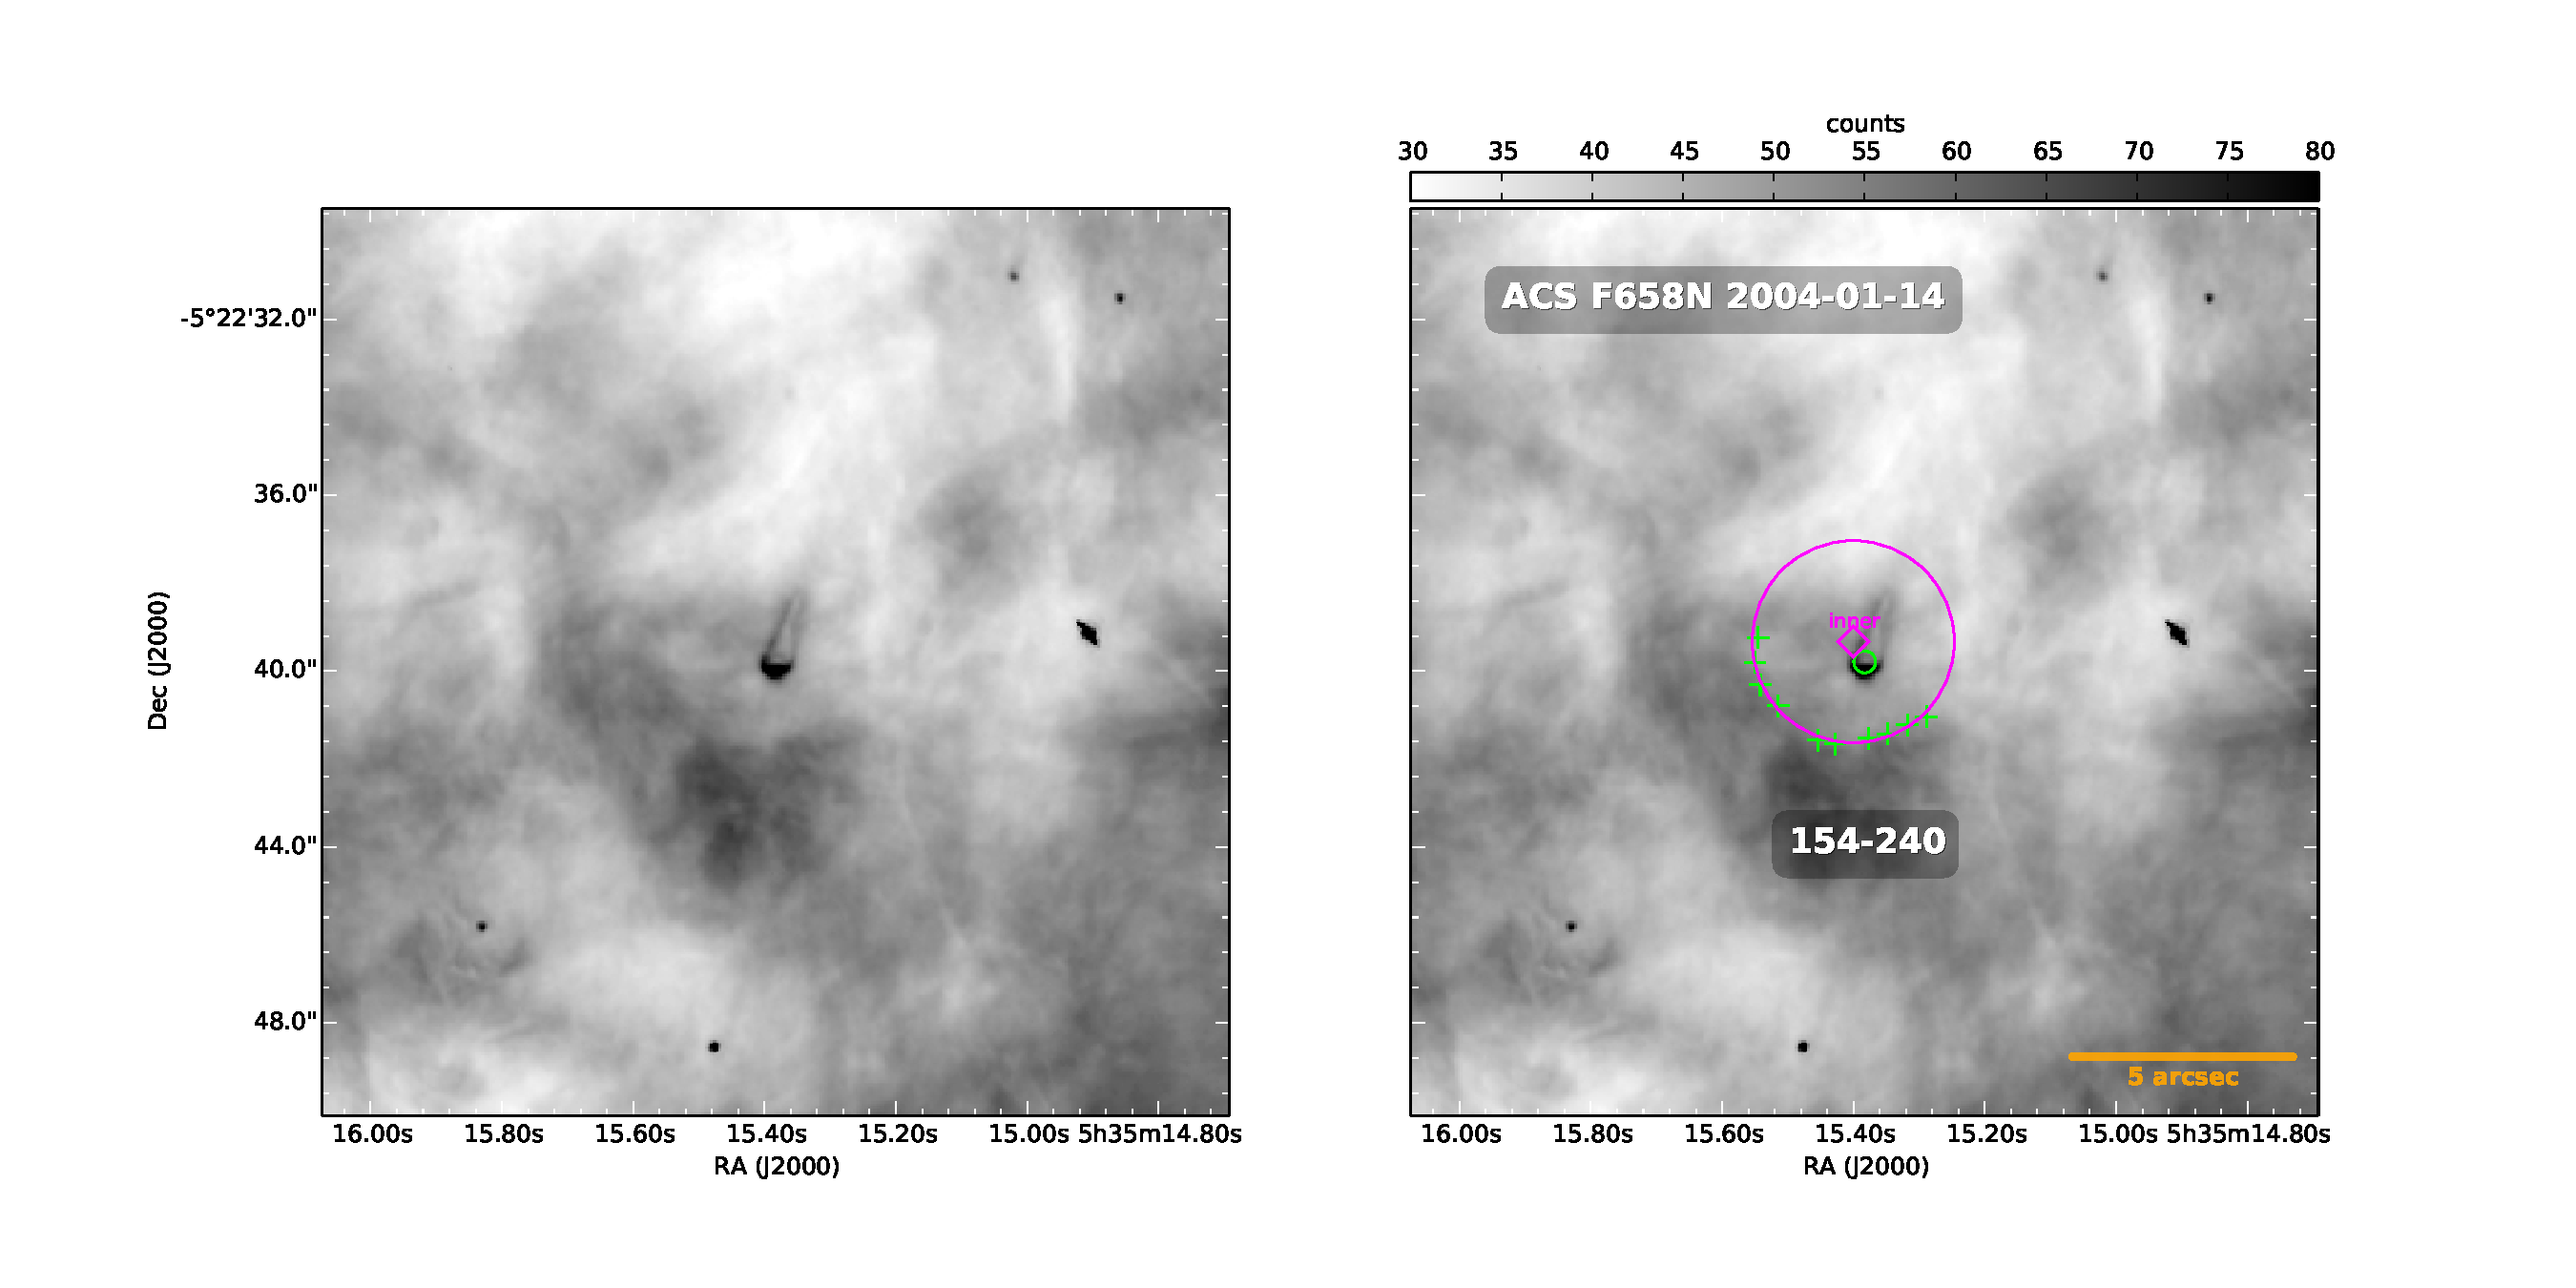
\includegraphics[width=\figwidth,  trim=60 50 100 50, clip]{j8oc01010_wcs/154-240-Bally_01-images.pdf}}\\
    \framebox{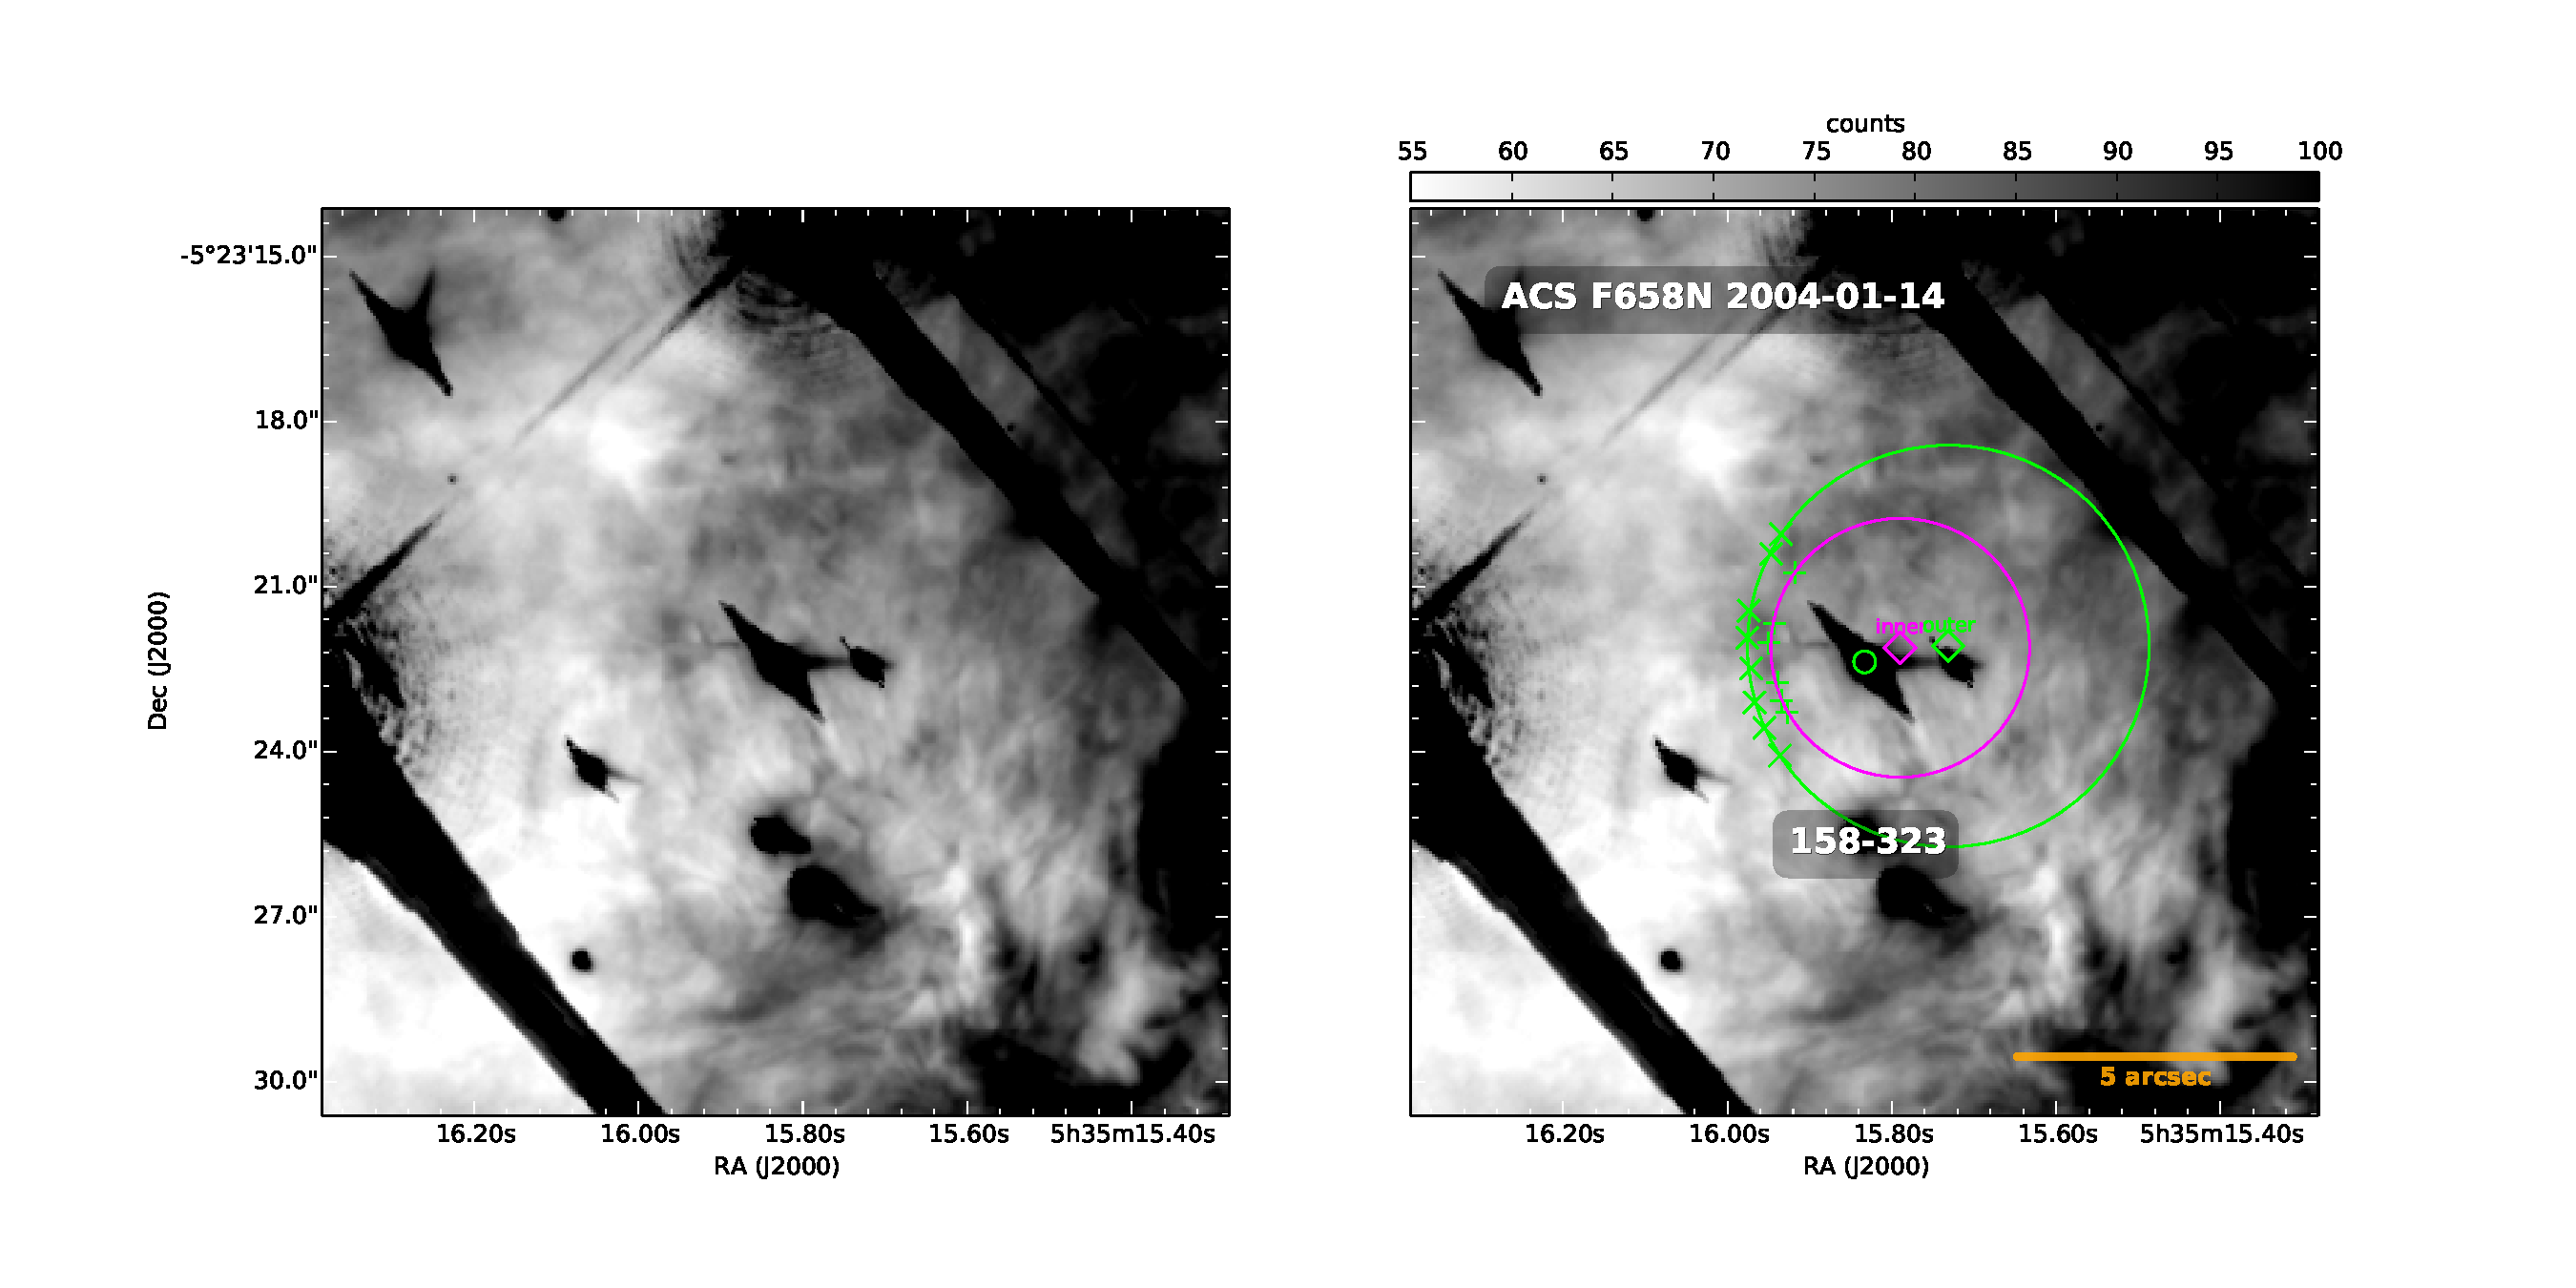
\includegraphics[width=\figwidth,  trim=60 50 100 50, clip]{j8oc01010_wcs/158-323-Bally_01-images.pdf}} 
    &\framebox{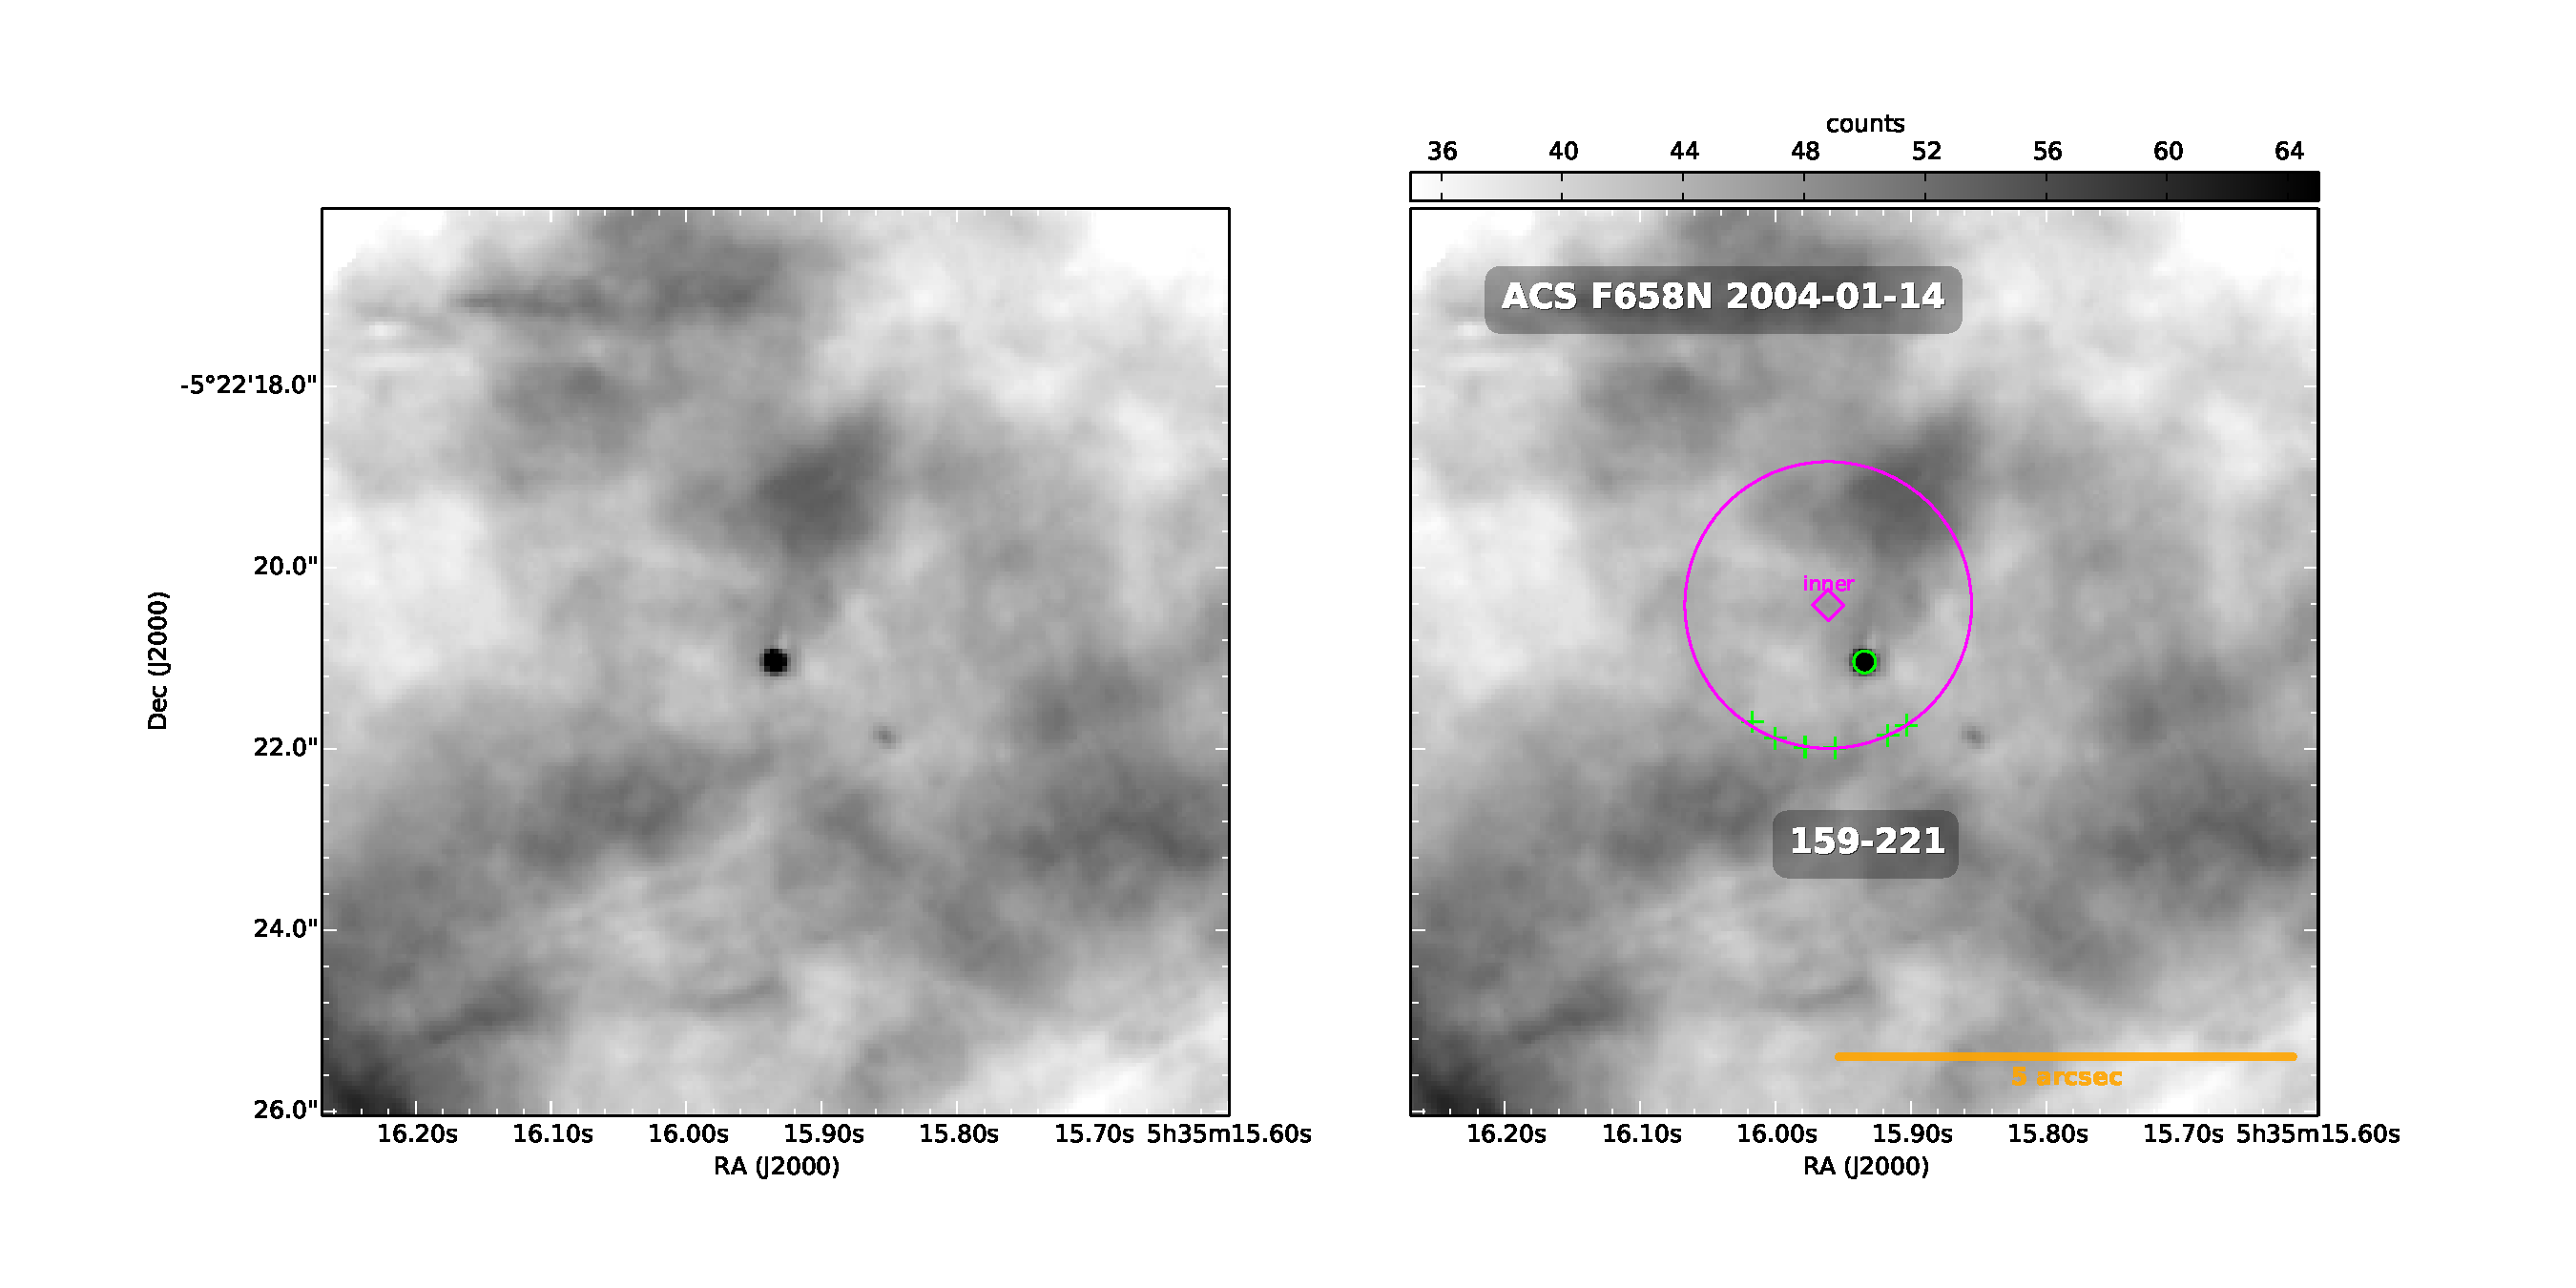
\includegraphics[width=\figwidth,  trim=60 50 100 50, clip]{j8oc01010_wcs/159-221-Bally_01-images.pdf}}\\
%   &\includegraphics[width=0.47\linewidth,  trim=60 50 100 50, clip]{j8oc01010_wcs/160-350-Bally_01-images.pdf}\\  
   \framebox{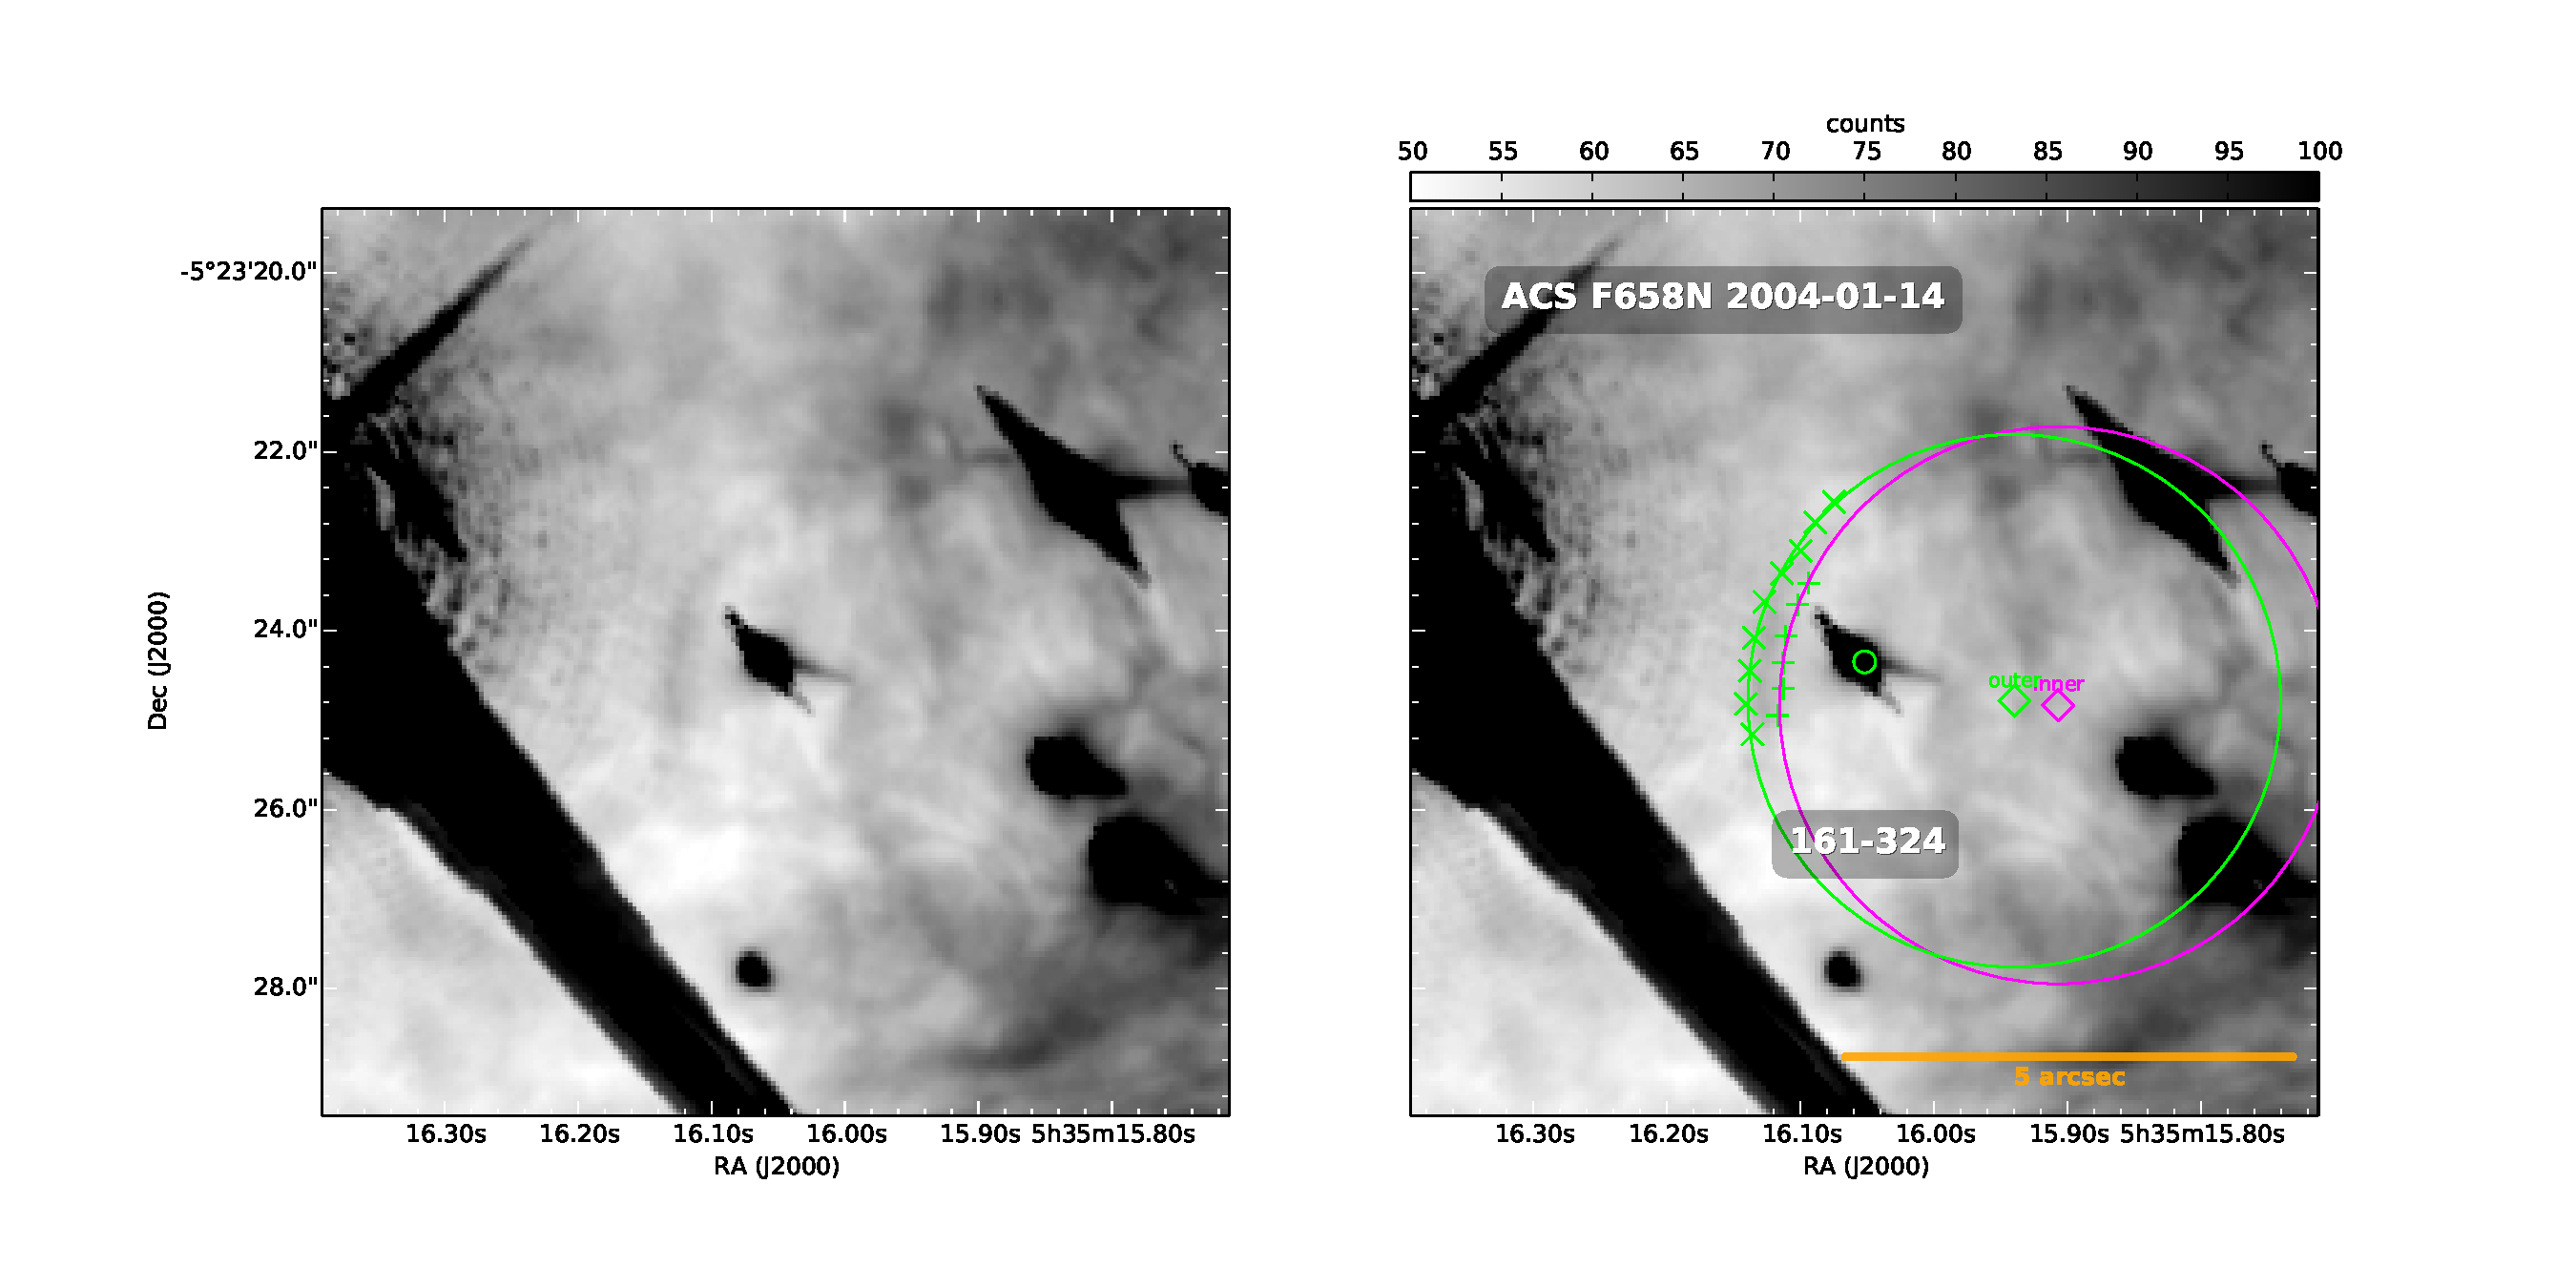
\includegraphics[width=\figwidth,  trim=60 50 100 50, clip]{j8oc01010_wcs/161-324-Bally_01-images.pdf}}
%    &\includegraphics[width=0.47\linewidth,  trim=60 50 100 50, clip]{j8oc06010_wcs/162-456-Bally_06-images.pdf}\\ \hline
    &\framebox{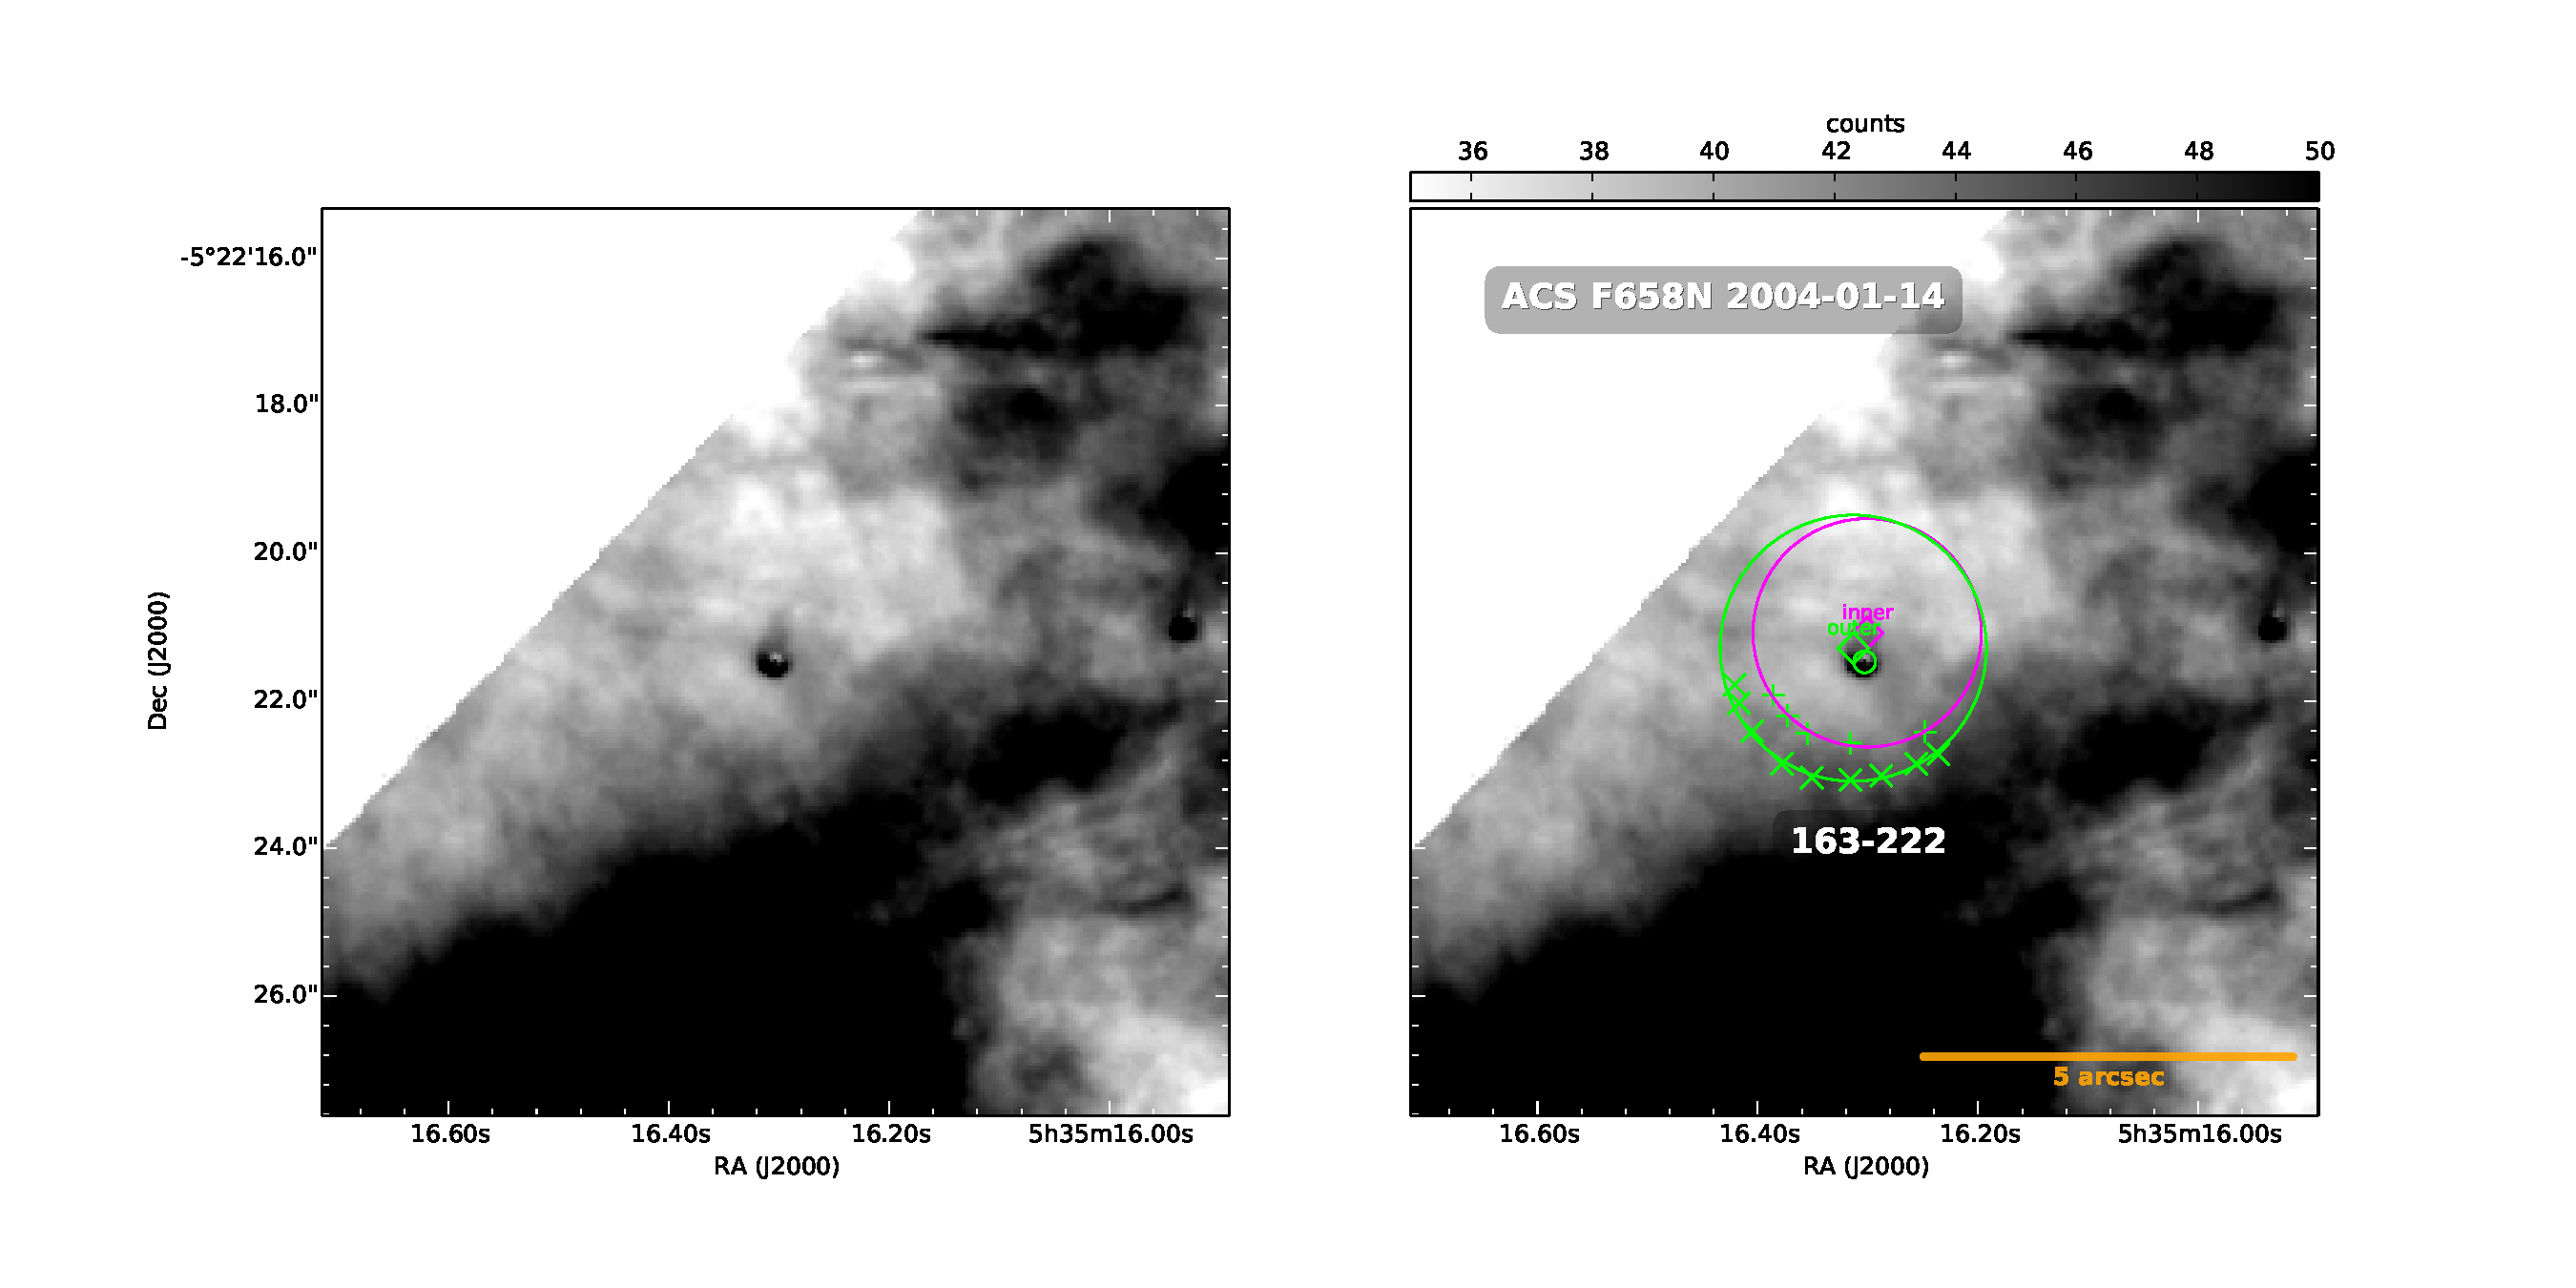
\includegraphics[width=\figwidth,  trim=60 50 100 50, clip]{j8oc01010_wcs/163-222-Bally_01-images.pdf}}\\
    \framebox{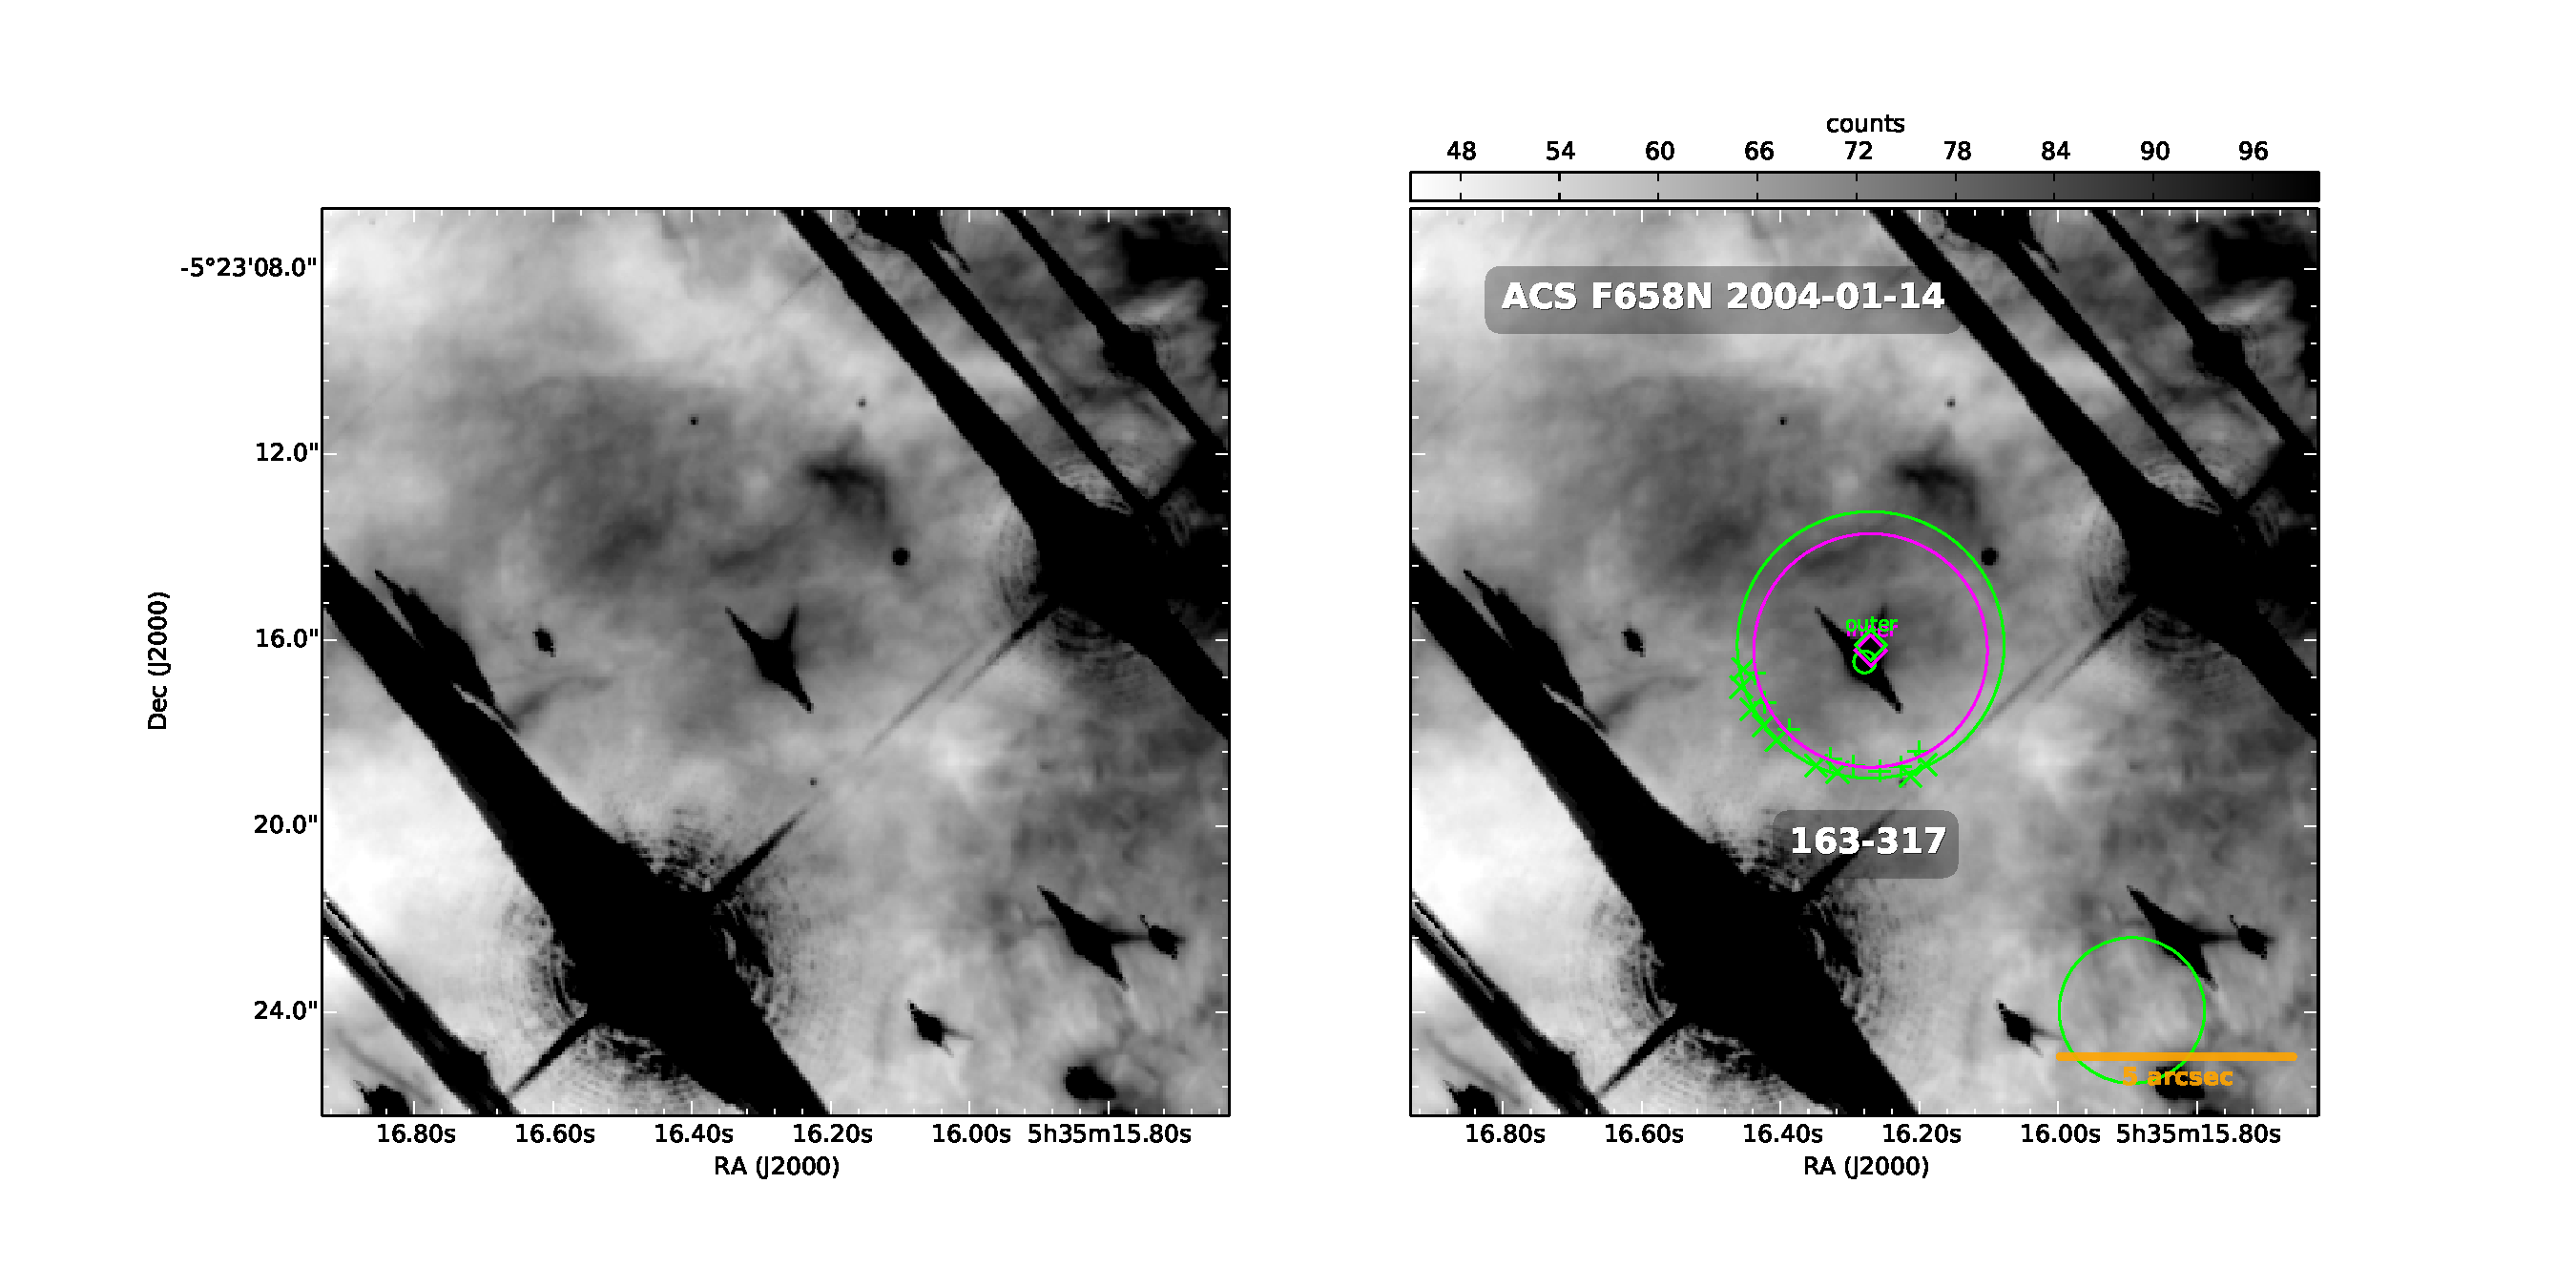
\includegraphics[width=\figwidth,  trim=60 50 100 50, clip]{j8oc01010_wcs/163-317-Bally_01-images.pdf}} 
    &\framebox{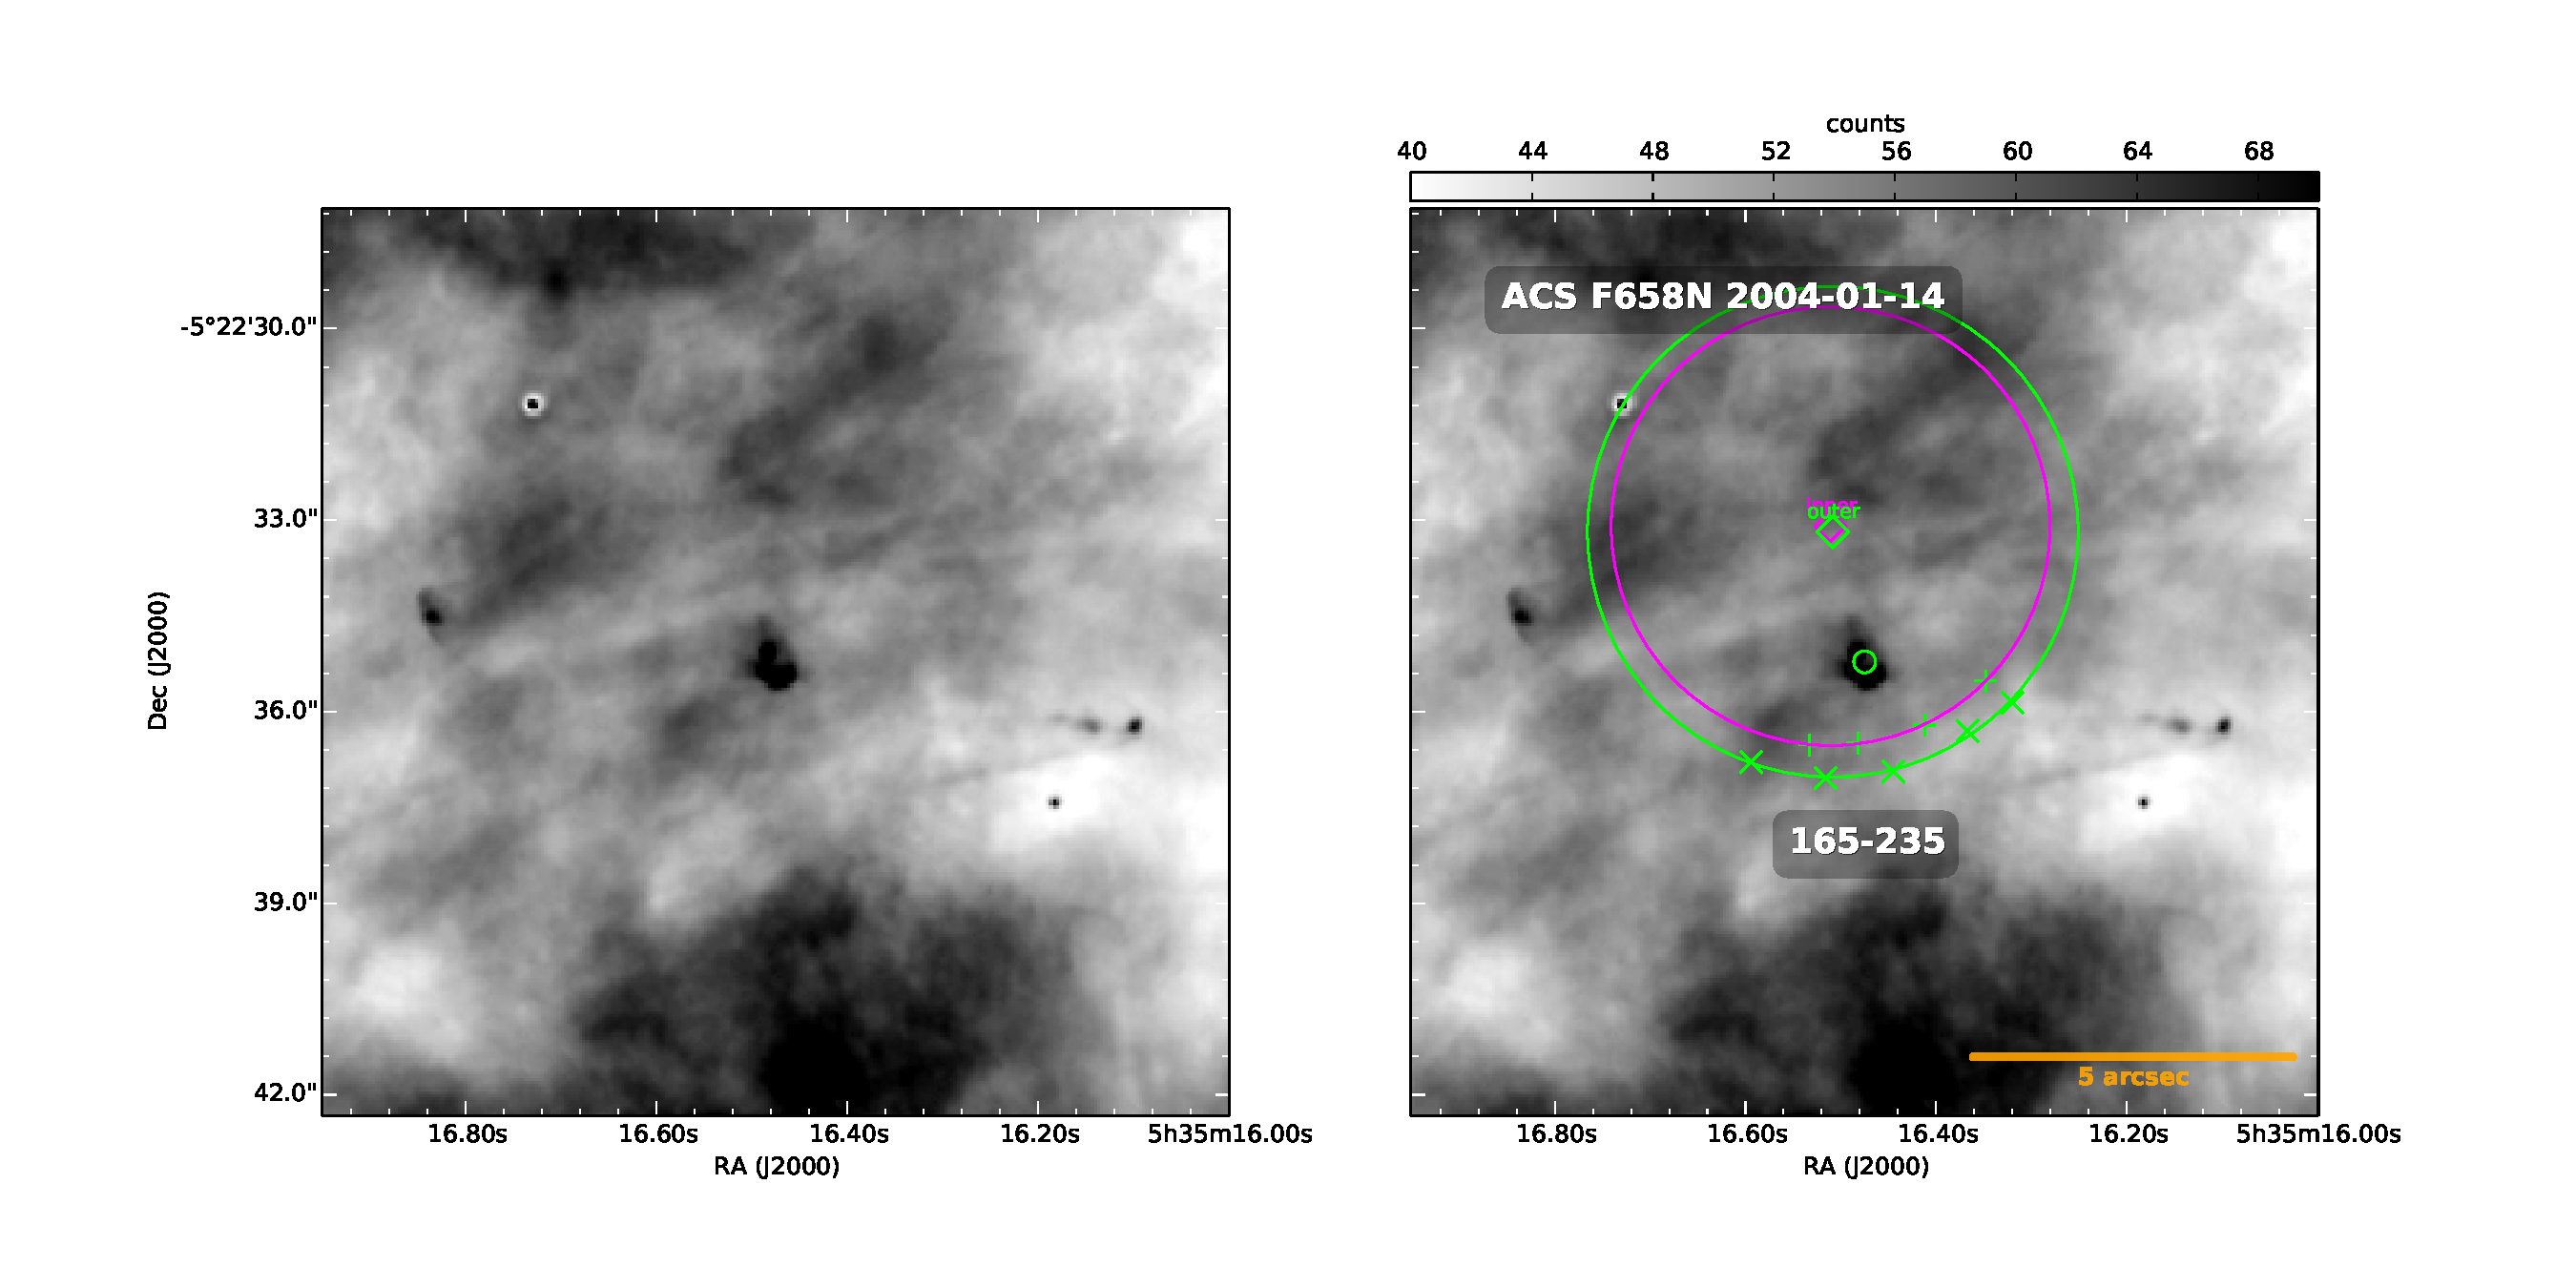
\includegraphics[width=\figwidth,  trim=60 50 100 50, clip]{j8oc01010_wcs/165-235-Bally_01-images.pdf}}\\
    \framebox{\includegraphics[width=\figwidth,  trim=60 50 100 50, clip]{j8oc01010_wcs/166-316-Bally_01-images.pdf}}
    &\framebox{\includegraphics[width=\figwidth,  trim=60 50 100 50, clip]{j8oc01010_wcs/167-317-Bally_01-images.pdf}}\\
\end{tabular}
\end{figure*}

\begin{figure*}
\setlength\tabcolsep{1.5pt}
\begin{tabular}{l l}
    \framebox{\includegraphics[width=\figwidth,  trim=60 50 100 50, clip]{j8oc01010_wcs/168-326-Bally_01-images.pdf}}
    &\framebox{\includegraphics[width=\figwidth,  trim=60 50 100 50, clip]{j8oc01010_wcs/168-326N-Bally_01-images.pdf}}\\
    \framebox{\includegraphics[width=\figwidth,  trim=60 50 100 50, clip]{j8oc01010_wcs/168-328-Bally_01-images.pdf}}
    &\framebox{\includegraphics[width=\figwidth,  trim=60 50 100 50, clip]{j8oc01010_wcs/169-338-Bally_01-images.pdf}}\\
    \framebox{\includegraphics[width=\figwidth,  trim=60 50 100 50, clip]{j8oc01010_wcs/170-249-Bally_01-images.pdf}}
    &\framebox{\includegraphics[width=\figwidth,  trim=60 50 100 50, clip]{j8oc01010_wcs/173-236-Bally_01-images.pdf}}\\
    \framebox{\includegraphics[width=\figwidth,  trim=60 50 100 50, clip]{j8oc01010_wcs/175-321-Bally_01-images.pdf}}
    &\framebox{\includegraphics[width=\figwidth,  trim=60 50 100 50, clip]{j8oc01010_wcs/177-341-Bally_01-images.pdf}}\\
    \framebox{\includegraphics[width=\figwidth,  trim=60 50 100 50, clip]{j8oc01010_wcs/173-342-Bally_01-images.pdf} }
    &\framebox{\includegraphics[width=\figwidth,  trim=60 50 100 50, clip]{j8oc01010_wcs/178-258-Bally_01-images.pdf}}\\
    \framebox{\includegraphics[width=\figwidth,  trim=60 50 100 50, clip]{j8oc01010_wcs/180-331-Bally_01-images.pdf} }
    &\framebox{\includegraphics[width=\figwidth,  trim=60 50 100 50, clip]{j8oc01010_wcs/189-329-Bally_01-images.pdf}}\\
\end{tabular}
\end{figure*}

\begin{figure*}
\setlength\tabcolsep{1.5pt}
\begin{tabular}{l l}
   \framebox{\includegraphics[width=\figwidth,  trim=60 50 100 50, clip]{j8oc14010_wcs/203-3039-Bally_14-images.pdf}}
    & \framebox{\includegraphics[width=\figwidth,  trim=60 50 100 50, clip]{j8oc06010_wcs/204-330-Bally_06-images.pdf}}\\
    \framebox{\includegraphics[width=\figwidth,  trim=60 50 100 50, clip]{j8oc02010_wcs/206-043-Bally_02-images.pdf}}
    &\framebox{\includegraphics[width=\figwidth,  trim=60 50 100 50, clip]{j8oc06010_wcs/212-400-Bally_06-images.pdf}}\\
    \framebox{\includegraphics[width=\figwidth,  trim=60 50 100 50, clip]{j8oc07010_wcs/261-3018-Bally_07-images.pdf}} 
    &\framebox{\includegraphics[width=\figwidth,  trim=60 50 100 50, clip]{j8oc06010_wcs/w266-558-Bally_06-images.pdf}} \\
    \framebox{\includegraphics[width=\figwidth,  trim=60 50 100 50, clip]{j8oc07010_wcs/305-811-Bally_07-images.pdf}}
     &\framebox{\includegraphics[width=\figwidth,  trim=60 50 100 50, clip]{j8oc08010_wcs/308-3036-Bally_08-images.pdf}}\\
    \framebox{\includegraphics[width=\figwidth,  trim=60 50 100 50, clip]{j8oc07010_wcs/LL5-Bally_07-images.pdf}}
    &\framebox{\includegraphics[width=\figwidth,  trim=60 50 100 50, clip]{j8oc08010_wcs/LL6-Bally_08-images.pdf}}\\
    \framebox{\includegraphics[width=\figwidth,  trim=60 50 100 50, clip]{j8oc08010_wcs/344-3020-Bally_08-images.pdf}}
    &\framebox{\includegraphics[width=\figwidth,  trim=60 50 100 50, clip]{wfpc2_64_f656n/LL7-Robberto_ACS_7l_f658n-images.pdf}}\\
\end{tabular}
\end{figure*}

\begin{figure}
\setlength\tabcolsep{1.5pt}
\begin{tabular}{l l }
    \framebox{\includegraphics[width=\figwidth,  trim=60 50 100 50, clip]{j8oc08010_wcs/362-3137-Bally_08-images.pdf}} 
 \end{tabular}  
\caption{Imágenes de \ha{}+\nii{} de los 73 objetos LL detectados en la Nebulosa de Orión. En ellas se puede apreciar la forma de los arcos, las estrellas jóvenes presecuencia principal en el interior y el ajuste de los círculos para los bordes internos y externos de la zona chocada. Imágenes tomadas con la cámara ACS-F658N como parte del programa GO-9825. }
  \label{fig:images}
\end{figure}

  
\section{Más sobre las observaciones: distancias, formas, tamaños y posiciones}
\label{sec:observations}

\begin{figure}
  \centering
  \includegraphics[width=\linewidth]{luis-programas/will-r0-vs-D}
  \caption{Radio de las cáscaras \(r0 = R_{0}\) (se tomaron los radios de las cáscaras externas) en función de la distancia proyectada. El tamaño de los símbolos indican la anchura relativa \(H=h/R_{0}\). La escala de colores representa el contraste de brillo superficial de \ha{} entre la cáscara y el fondo.}
  \label{fig:radio-cas}
\end{figure} 

Como se ha dicho anteriormente usando éstas observaciones hemos medido parámetros observacionales con el propósito de caracterizar los objetos LL y los choques de proa de los proplyds. En este orden de ideas hemos medido la distancia \(D\) de la fuente a \thC{}, la anchura \(h\) de la cáscara y los radios característicos, \(R_{0}\) y \(R_{c}\) tanto de los límites internos y externos de la cáscara chocada. La tabla~\ref{tab:test} es el resultado final de tales mediciones.\\

\begin{figure}
  \centering
  \includegraphics[width=\linewidth]{luis-programas/will-H-vs-q}
  \caption{Ancho de la cáscara chocada \(h\) dividida entre el radio del choque externo \(r0 = R_{0}\) a lo largo del eje de simetría, para obtener el ancho relativo \(H\), en función de  \(r0 = R_{0}\) normalizado con \(D\), esto es el término \(q\), que es un indicativo de los tamaños relativos de los objetos LL y choques de los proplyds. El color de los puntos indica la distancia proyectada desde la fuente al Trapecio (ver el panel de colores de la izquierda). Por último, cabe mencionar que el tamaño de los símbolos hace referencia a los valores del radio del borde característico  \(R_{0}\), el cual es el radio desde la estrella presecuencia principal al choque externo a lo largo del eje de simetría.}
  \label{fig:thikness}
\end{figure} 

 En la figura \ref{fig:radio-cas} se puede ver que el radio de las cáscaras (distancia de la estrella joven a los choques) no depende de la distancia proyectada del Trapecio, debido a que existe una dispersión muy marcada en los valores de estas mediciones en nuestras muestras. Mientras que en la figura~\ref{fig:thikness}, se logra apreciar que los choques de proa situados a grandes distancias  proyectadas desde \thC{}, tienden a tener  pequeños tamaños en términos relativos, porque hemos tomado el cociente \(q = R_{0}/D\) para indicar el tamaño de los objetos que es diferente a los valores medidos para el radio \(R_{0}\).  Entonces el cociente \(q = R_{0}/D\) es menor para estas distancias\footnote{Se ha tomado \(R_{0}\), como el radio del borde externo de la cáscara chocada.}, esto es en comparación a los objetos más distantes los cuales muestran que el radio relativo \(q\) es más grande, indicando por tanto que son de mayores tamaños relativamente hablando. Por otro lado esta figura también nos muestra que los choques de proa más distantes tienden a tener cáscaras más anchas que los arcos interiores, es decir que para los objetos de menor tamaño sus cáscaras chocadas son de mayor anchura. Esto es debido por un lado a que muchos de estos objetos LL tienen doble cáscara y también posiblemente podría deberse a que estos objetos están interactuando con el flujo de champaña proveniente del núcleo de la nebulosa (ver figura~\ref{fig:images}).\\ 

\begin{figure}
  \centering
  \includegraphics[width=\linewidth]{luis-programas/will-A-vs-q}
  \caption{Radios de curvaturas de los choques externos \(R_{c}\) dividido entre \(R_{0}\). A esta fracción la hemos llamado \(A\), en función de \(q\), como una forma para establecer que tan abiertos o cerrados son las alas de los choques LL. La escala de colores representa la distancia de los objetos a \thC{} y el tamaño de los símbolos es un indicativo de la longitud del radio \(R_{0}\).}
  \label{fig:radii-curvatures}
\end{figure} 

Es de notar que tenemos valores variados para los radios de curvaturas y puesto que con estos parámetros podemos hacernos una idea de la forma de los choques. Entonces tenemos que en la figura~\ref{fig:radii-curvatures} es perceptible que los radios de curvaturas\footnote{También se ha tomado el radio de curvatura externo.} normalizados con los radios axiales \(R_{0}\), esto es la fracción \(A=R_{c}/R_{0}\), aumentan con la distancia a la estrella ionizante; entonces es coherente argumentar que los choques ubicados en la regiones externas de la nebulosa tienden a mostrar arcos muy abiertos en sus formas. Es el caso de los objetos LL1, LL2, LL3, LL4, LL5, LL6, LL7,  203-3039, w266-558 y w000-400 por citar algunos. Es importante señalar que las cáscaras más abiertas están asociadas con jets perpendiculares al eje de los choques de proa, esto sucede con las cáscaras de los objetos LL2, LL6 y 203-3039. Los choques de proa situados en las cercanías de \thC{}, es decir a cortas distancias, tienen valores de \(A\) más pequeños en comparación a los valores de esta fracción para los objetos más distantes. Nos enfrentamos con el hecho de que los choques de proa ubicados en el interior de la nebulosa, van a tener arcos más cerrados, como sucede con 108-326, 142-301, 177-341, 167-317, 168-326N, 168-328, 173-236, 175-321, 180-331, entre otros (ver los valores de los radios de curvatura en la tabla~\ref{tab:test}  y las posiciones de los arcos es las figuras~\ref{fig:position-arc} y~\ref{fig:position-arc-zoom}).\\  

\begin{figure}
  \centering
  \includegraphics[width=\linewidth]{ll-pos-image}
  \caption{Posiciones de los arcos LL superpuestos en una imagen de \ha{} de la Nebulosa de Orión. Los arcos con las flechas representan los objetos LL y los proplyds con sus respectivos choques estacionarios, de nuestro catálogo. Las flechas verdes y violetas indican la orientación de los arcos externos e internos respectivamente. Además se han incluidos los proplyds y otros objetos del catálogo de \citet{Ricci:2008}, donde los puntos de color rojo representan los clásicos proplyds, los puntos de color negro representan los típicos discos de acreción, los de color verde representan jets radiativos sin evidencia de la presencia de discos ionizados y los símbolos de color cian son nebulosas de reflexión sin emisión externa de gas ionizado. El cuadro en la zona del Trapecio de la imagen es la región ampliada en la figura~\ref{fig:position-arc-zoom}.}
  \label{fig:position-arc}
\end{figure}

En la figura~\ref{fig:position-arc} se ilustran las posiciones de los arcos LL de nuestro catálogo en la Nebulosa de Orión, además se muestran las posiciones con simbolos de color rojo de los proplyds del catálogo de \citet{Ricci:2008}. Incluimos estos objetos para mostrar que muchos proplyds de la Nebulosa de Orión no tienen choques de proa asociados. Se observa que los objetos LL están distribuidos por toda la nebulosa, esto es que existe una gran cantidad de arcos de emisión en el noroeste y suroeste de la misma, una cantidad un poco menor de estos choques se observan en el sureste y es muy poco el número de arcos LL situados en el noreste de la nebulosa; además se indican las orientaciones de los arcos internos y externos de estos objetos. Los objetos LL y los choques de proa de los proplyds de la figura~\ref{fig:position-arc} de las que estamos hablando, son aquellos ubicados a largas distancias del Trapecio, puesto que en el interior de la nebulosa el mapa está muy saturado y no se logran ver de manera clara las posiciones y orientaciones de los arcos en esta región. Para eso contamos con la figura~\ref{fig:position-arc-zoom} el cual es una ampliación de la región donde se encuentran las estrellas masivas del Trapecio, en ella es posible ver las posiciones de los proplyds y las orientaciones de sus respectivos choques en el interior de la nebulosa de una forma más clara. Las direcciones de las flechas de los arcos radiativos LL en las afueras de la nebulosa sugieren a simple vista que estos arcos están orientados hacia el núcleo de la Nebulosa de Orión, de la misma forma los choques de los proplyds en las regiones internas al parecer están orientados hacia \thC{}, es decir en la dirección radial.\\

\begin{figure}
  \centering
  \includegraphics[width=\linewidth]{ll-pos-image-zoom}
  \caption{Posiciones de los arcos LL. Con un zoom de una pequeña área en el núcleo de la nebulosa. Las flechas y los colores de los símbolos representan los mismos conceptos y objetos que en la figura~\ref{fig:position-arc}.}
  \label{fig:position-arc-zoom}
\end{figure}

\newpage
\newcommand\TestTableHeader{
  \hline\hline
Objeto & \(\mathrm{A.R.}\) & \(\mathrm{Decli}\) & \(D\) & \(h\) & \(R_{0}(\mathrm{out})\) & \(R_{0}(\mathrm{in})\) & \(R_{c}(\mathrm{out})\) & \(R_{c}(\mathrm{in})\) \\
  %Object & \(D\) &   \(R_{\mathrm{out}}\) & \(R_{\mathrm{in}}\) \\
  \hline 
}

\begin{longtable}{lllcccccc}
  \caption{Distancias, tamaños y formas de los choques de proa en la Nebulosa de Orión. Las unidades de la distancia y los radios están en [arcsec]. \label{tab:test}}\\
  \TestTableHeader\endfirsthead 
  \caption[]{continuación  }\\
  \TestTableHeader\endhead
  \hline \endfoot
  %\begin{table}
%\begin{tabular}{ccccccccc}
%Object & RA & Dec & D & h & R_out & R_in & Rc_out & Rc_in \\
4285-458 & 5:34:28.520 & -5:24:57.88 & 721.182 & 0.0 & 1.913 & -- & 4.344 & -- \\
LL3 & 5:34:40.807 & -5:26:38.54 & 566.331 & 1.83 & 3.119 & 1.284 & 6.544 & 3.085 \\
LL2 & 5:34:40.860 & -5:22:42.20 & 532.124 & 1.133 & 4.035 & 2.074 & 27.93 & 13.844 \\
LL4 & 5:34:42.719 & -5:28:37.20 & 593.107 & 0.992 & 2.415 & 1.422 & 11.787 & 4.952 \\
4468-605 & 5:34:46.75775 & -5:26:04.81750 & 471.3 & 1.199 & 2.469 & 1.331 & 7.109 & 2.223 \\
4578-251 & 5:34:57.79275 & -5:22:51.09500 & 279.493 & 0.533 & 1.846 & 1.188 & 3.52 & 2.074 \\
4582-635 & 5:34:58.16675 & -5:26:35.12750 & 333.372 & 0.455 & 1.106 & 0.682 & 2.931 & 2.056 \\
w000-400 & 5:34:59.56575 & -5:24:00.14500 & 254.035 & 0.675 & 1.465 & 0.795 & 4.369 & 2.432 \\
w005-514 & 5:35:00.46775 & -5:25:14.29750 & 262.718 & 0.437 & 1.651 & 1.201 & 3.449 & 2.032 \\
w005-514 & 5:35:00.471 & -5:25:14.21 & 262.637 & 0.424 & 1.672 & 1.171 & 2.239 & 2.213 \\
w012-407 & 5:35:01.17375 & -5:24:06.67750 & 231.47 & 1.234 & 2.289 & 0.953 & 6.743 & 4.264 \\
w014-414 & 5:35:01.37175 & -5:24:13.36750 & 229.954 & 0.696 & 1.211 & 0.373 & 2.185 & 1.615 \\
022-635 & 5:35:02.200 & -5:26:35.33 & 286.472 & 0.341 & 1.104 & 0.75 & 4.456 & 2.29 \\
w030-524 & 5:35:03.00375 & -5:25:24.35750 & 234.087 & 0.315 & 0.626 & 0.288 & 2.559 & 1.541 \\
041-637 & 5:35:04.060 & -5:26:37.06 & 267.84 & 0.766 & 1.937 & 1.189 & 4.395 & 3.232 \\
042-628 & 5:35:04.19875 & -5:26:27.59750 & 259.592 & 1.339 & 3.069 & 1.76 & 6.901 & 3.606 \\
w044-527 & 5:35:04.427 & -5:25:27.39 & 217.945 & 0.851 & 2.13 & 0.78 & 3.25 & 1.527 \\
049-143 & 5:35:04.945 & -5:21:42.92 & 197.821 & 0.56 & 1.173 & 0.625 & 4.178 & 0.662 \\
051-024 & 5:35:05.131 & -5:20:24.32 & 245.01 & 0.269 & 1.186 & 0.895 & 2.287 & 1.663 \\
LL1 & 5:35:05.63675 & -5:25:19.44750 & 198.626 & 1.128 & 3.057 & 1.904 & 8.721 & 7.132 \\
065-502 & 5:35:06.53975 & -5:25:01.50750 & 177.288 & 1.214 & 1.422 & 0.491 & 7.737 & 2.31 \\
066-3251 & 5:35:06.56919 & -5:32:51.43000 & 587.491 & 0.0 & 1.068 & -- & 1.588 & -- \\
066-652 & 5:35:06.588 & -5:26:52.38 & 255.852 & 0.102 & 0.028 & -0.075 & 0.575 & 0.6 \\
w069-601 & 5:35:06.90775 & -5:26:00.57750 & 212.194 & 0.423 & 0.853 & 0.405 & 2.723 & 1.773 \\
072-134 & 5:35:07.20375 & -5:21:34.29500 & 174.737 & 2.419 & 4.69 & 2.261 & 17.626 & 7.286 \\
w073-227 & 5:35:07.26975 & -5:22:26.49750 & 147.268 & 0.696 & 1.626 & 0.811 & 6.462 & 3.979 \\
074-229 & 5:35:07.384 & -5:22:28.92 & 144.777 & 0.596 & 1.357 & 0.79 & 1.601 & 0.748 \\
083-435 & 5:35:08.29275 & -5:24:34.85750 & 140.892 & 0.579 & 1.247 & 0.544 & 2.005 & 0.664 \\
101-233 & 5:35:10.133 & -5:22:32.60 & 105.936 & 0.419 & 2.458 & 2.111 & 4.356 & 4.206 \\
102-157 & 5:35:10.25075 & -5:21:57.11750 & 125.297 & 0.45 & 0.796 & 0.402 & 5.03 & 3.542 \\
106-245 & 5:35:10.576 & -5:22:44.69 & 94.703 & 0.38 & 0.627 & 0.228 & 2.476 & 1.121 \\
109-246 & 5:35:10.89575 & -5:22:46.31750 & 89.677 & 0.704 & 1.948 & 1.322 & 10.638 & 7.325 \\
117-421 & 5:35:11.650 & -5:24:21.41 & 92.066 & 0.0 & -- & 0.71 & -- & 0.927 \\
116-3101 & 5:35:11.65419 & -5:31:01.03000 & 463.921 & 0.44 & 1.452 & 1.004 & 2.695 & 1.574 \\
119-3155 & 5:35:11.926 & -5:31:53.30 & 515.101 & 1.002 & 3.015 & 1.951 & 6.727 & 5.11 \\
121-434 & 5:35:12.12175 & -5:24:33.75750 & 95.578 & 0.39 & 0.757 & 0.344 & 1.413 & 0.688 \\
124-131 & 5:35:12.383 & -5:21:31.41 & 126.201 & 1.733 & 4.477 & 2.744 & 5.95 & 10.415 \\
131-046 & 5:35:13.05537 & -5:20:45.78625 & 164.46 & 2.168 & 3.546 & 0.999 & 7.325 & 5.645 \\
132-053 & 5:35:13.202 & -5:20:52.59 & 157.312 & 0.392 & 0.718 & 0.317 & 1.803 & 0.676 \\
136-3057 & 5:35:13.60719 & -5:30:57.56000 & 456.925 & 4.51 & 10.133 & 4.907 & 18.706 & 10.203 \\
138-3024 & 5:35:13.79919 & -5:30:24.40000 & 423.642 & 1.107 & 3.893 & 2.744 & 8.539 & 4.787 \\
142-301 & 5:35:14.158 & -5:23:01.00 & 39.672 & 0.6 & 2.422 & 1.822 & 6.062 & 4.547 \\
154-225 & 5:35:15.367 & -5:22:25.31 & 59.219 & 0.584 & 1.287 & 0.636 & 3.421 & 1.051 \\
154-240 & 5:35:15.383 & -5:22:39.79 & 45.303 & 0.0 & -- & 1.72 & -- & 2.3 \\
158-323 & 5:35:15.831 & -5:23:22.51 & 8.338 & 0.206 & 1.849 & 1.643 & 2.92 & 2.354 \\
159-221 & 5:35:15.934 & -5:22:21.04 & 61.862 & 0.0 & -- & 0.834 & -- & 1.582 \\
160-350 & 5:35:15.958 & -5:23:49.68 & 27.906 & 0.067 & 0.109 & 0.042 & 0.598 & 0.294 \\
161-324 & 5:35:16.056 & -5:23:24.33 & 5.295 & 0.255 & 1.159 & 0.904 & 3.013 & 2.027 \\
162-456 & 5:35:16.182 & -5:24:56.39 & 93.914 & 0.086 & 0.294 & 0.208 & 0.853 & 0.785 \\
163-317 & 5:35:16.282 & -5:23:16.63 & 6.111 & 0.395 & 2.323 & 1.928 & 4.904 & 4.437 \\
163-222 & 5:35:16.303 & -5:22:21.47 & 61.071 & 0.356 & 1.538 & 1.108 & 1.805 & 1.549 \\
165-235 & 5:35:16.475 & -5:22:35.22 & 47.325 & 0.472 & 1.776 & 1.225 & 3.842 & 3.437 \\
166-316 & 5:35:16.607 & -5:23:16.16 & 7.149 & 0.279 & 0.694 & 0.415 & 1.191 & 0.851 \\
167-317 & 5:35:16.739 & -5:23:16.50 & 7.974 & 0.706 & 1.96 & 1.254 & 3.286 & 2.052 \\
168-328 & 5:35:16.757 & -5:23:28.05 & 7.787 & 0.272 & 1.062 & 0.789 & 1.315 & 0.799 \\
168-326N & 5:35:16.835 & -5:23:25.97 & 7.493 & 0.111 & 0.229 & 0.118 & 1.044 & 0.79 \\
168-326 & 5:35:16.839 & -5:23:26.32 & 7.712 & 0.196 & 0.947 & 0.737 & 3.044 & 3.011 \\
169-338 & 5:35:16.880 & -5:23:38.02 & 17.138 & 0.351 & 1.031 & 0.68 & 2.037 & 0.719 \\
170-249 & 5:35:16.967 & -5:22:48.44 & 35.162 & 0.777 & 3.225 & 2.448 & 6.92 & 4.755 \\
173-342 & 5:35:17.324 & -5:23:41.39 & 23.465 & 0.462 & 1.29 & 0.828 & 3.312 & 1.719 \\
173-236 & 5:35:17.352 & -5:22:35.73 & 48.956 & 0.753 & 2.28 & 1.527 & 1.364 & 1.935 \\
175-321 & 5:35:17.458 & -5:23:21.06 & 16.026 & 0.598 & 2.031 & 1.384 & 2.478 & 2.626 \\
177-341 & 5:35:17.667 & -5:23:40.98 & 26.543 & 0.749 & 3.813 & 3.064 & 4.247 & 3.867 \\
178-258 & 5:35:17.819 & -5:22:58.06 & 32.473 & 0.524 & 1.479 & 0.923 & 3.944 & 3.43 \\
180-331 & 5:35:18.033 & -5:23:30.82 & 25.909 & 0.326 & 1.44 & 1.114 & 2.361 & 1.772 \\
189-329 & 5:35:18.868 & -5:23:28.88 & 37.556 & 0.856 & 1.397 & 0.538 & 6.318 & 0.833 \\
203-3039 & 5:35:20.289 & -5:30:39.38 & 440.716 & 3.06 & 5.384 & 1.761 & 17.897 & 14.501 \\
204-330 & 5:35:20.402 & -5:23:30.01 & 60.389 & 0.221 & 0.333 & 0.112 & 1.336 & 1.281 \\
206-043 & 5:35:20.561 & -5:20:43.11 & 171.159 & 0.443 & 1.609 & 1.117 & 2.186 & 2.077 \\
212-400 & 5:35:21.181 & -5:24:00.46 & 80.988 & 0.213 & 1.075 & 0.844 & 0.831 & 0.518 \\
261-3018 & 5:35:26.16875 & -5:30:18.01750 & 440.4 & 2.591 & 4.986 & 2.514 & 33.288 & 3.586 \\
w266-558 & 5:35:26.618 & -5:25:58.29 & 218.155 & 0.775 & 1.88 & 1.127 & 7.761 & 1.506 \\
305-811 & 5:35:30.43675 & -5:28:11.23750 & 356.86 & 0.8 & 1.721 & 0.891 & 4.924 & 3.993 \\
308-3036 & 5:35:30.79475 & -5:30:36.25250 & 484.126 & 1.125 & 2.557 & 1.438 & 4.497 & 1.782 \\
LL5 & 5:35:31.39775 & -5:28:16.35750 & 369.536 & 1.487 & 2.963 & 1.456 & 11.577 & 3.517 \\
LL6 & 5:35:32.86575 & -5:30:21.45250 & 485.816 & 2.049 & 3.628 & 1.626 & 29.899 & 14.201 \\
344-3020 & 5:35:34.36275 & -5:30:20.56250 & 496.758 & 0.947 & 1.659 & 0.673 & 3.155 & 4.423 \\
LL7 & 5:35:35.126 & -5:33:49.16 & 686.232 & 1.46 & 6.998 & 5.533 & 17.958 & 10.306 \\
362-3137 & 5:35:36.34775 & -5:31:37.75250 & 577.964 & 1.465 & 3.121 & 1.572 & 4.245 & 2.222 \\
%\end{tabular}
%\end{table}

\end{longtable}


\section{Detalles sobre las posiciones angulares y poblaciones de choques LL y proplyds }
\label{sec:disc}

\begin{figure}
  \centering
  \includegraphics[width=\linewidth, clip]{luis-programas/will-PA-vs-PA}
  \caption{Angulo entre el eje del choque de proa y la dirección radial (este último es en dirección a \thC{}), en función de la posición angular del eje desde \thC{} a la fuente en el plano del cielo, es decir tomando las coordenadas cartesianas (\(x, y\)). La línea azul y vertical representa el ángulo ``0'' entre las dos posiciones angulares. La escala de colores representa la distancia proyectada desde los objetos LL al Trapecio y el tamaño de los símbolos al igual que en las anteriores gráficas representa el radio característico \(R_{0}\).}
 \label{fig:pos-angular}
\end{figure}

Las mediciones de las posiciones de los 73 arcos de emisión detectados en la Nebulosa de Orión han permitido indicar las orientaciones de los choques, que entre otras cosas siguen la dirección del flujo externo de la nebulosa, como resultado intrínseco de la interacción de este con el viento interno de la estrella T-Tauri o proplyd. De acuerdo a las orientaciones mostradas en las figuras \ref{fig:position-arc} y \ref{fig:position-arc-zoom} de los arcos en la nebulosa, podemos pensar que el flujo proveniente del núcleo de la nebulosa es aproximadamente radial, como se ha interpretado en la sección \S\ref{sec:images}.\\

 No obstante, en la figura \ref{fig:pos-angular} se ilustran de manera más estricta que tanto siguen la dirección radial las orientaciones de los arcos radiativos en las regiones internas y externas  de la nebulosa, considerando la dirección radial, como la línea imaginaria que va desde la fuente hasta \thC{}. Para ello, con los valores medidos de las posiciones angulares de las fuentes a \thC{}, es decir el ángulo formado por la dirección radial en el plano del cielo (\(x, y\)), junto con los valores medidos de las posiciones angulares de los ejes de los choques o eje de simetría en el plano del cielo, se ha estimado el desplazamiento angular del eje del choque con respecto a la línea imaginaria trazada desde la fuente a \thC{}, tomando este último como eje de referencia\footnote{A excepción de los choques de proa producidos por la interacción de los vientos de dos proplyds, donde se ha tomado como eje de referencia la dirección de uno de los proplyds con respecto al otro.}; en otras palabras se ha calculado el ángulo entre el eje del choque y la dirección radial. Los resultados han mostrado que las direcciones de los ejes de los choques no son estrictamente radiales, puesto que están desplazadas en un intervalo que va desde \(0^{\circ}\) a \(-30^{\circ}\) en el noroeste y noreste de la nebulosa, mientras que los ejes de los arcos ubicados en el sureste y suroeste están desplazados en un intérvalo de ángulo que va desde \(0^{\circ}\) a \(30^{\circ}\). Estos ángulos positivos y negativos en los diferentes cuadrantes de la nebulosa indican un desplazamiento hacia la izquierda de la dirección radial, de los ejes de simetría de los choques de proa, es decir que no es estrictamente radial la orientación de los arcos. \\


\begin{figure}
\centering
\begin{tabular}{l l}
  (\textit{a})\\
  \includegraphics[width=0.76\linewidth]{proplyd-star-ratio}\\
  (\textit{b})\\
  \includegraphics[width=0.76\linewidth]{bowshock-proplyd-ratio}
  \end{tabular}  
  \caption{(\textit{a})~Fracción de todas las estrellas opticamente visibles que son proplyds (simbolos circulares oscuros) o que tienen choques de proa (símbolos cuadrados claros) como una función de la separación proyectada desde el Trapecio. (\textit{b})~Relación entre el número de choques de proa y el número de proplyds en función de la separación proyectada desde el Trapecio. Los símbolos circulares y oscuros representan todos los choques de nuestro catálogo (a excepción de los choques producidos pos la interacción de dos proplyds) mientras que los símbolos cuadrados y claros indican estos mismos choques de proa pero sólo aquellos asociados con conocidos y supuestos proplyds.}
\label{fig:bow-proplyd-star-ratios}
\end{figure}

En la figura~\ref{fig:bow-proplyd-star-ratios}, se observa que la fracción de proplyds entre el número de estrellas cae relativamente con facilidad con la distancia proyectada a \thC{}, mostrando una repentina caida después de unos 200~arcsec.\\

Por otro lado el cociente entre los choques de proa y los proplyds parece tener tres picos separados. En este orden de ideas, para distancias muy pequeñas se puede ver que el primer pico corresponde a la interacción del viento estelar con el viento ionizado de los proplyds, a continuación hay una escacez de choques de proa hasta el segundo pico cerca de unos 4~arcmin. Por último se puede apreciar que  a grandes distancias, donde podría haber un tercer pico dominan el número de objetos que no son proplyds.\\

 Una explicación alternativa para lo planteado anteriormente, podría ser que en este tercer pico todos los objetos son proplyds, pero como se piensa que a grandes distancias no se sabe con certeza que clase de objetos están originando los vientos en una escala más pequeña, entonces estaríamos subestimando  la fracción de proplyds para estas grandes distancias.\\

También hay evidencia de tres distintas poblaciones de la distribución azimutal alrrededor del Trapecio. Para el grupo ubicado a 4~arcmin de separación son principalmente aquellos objetos del oeste de la nebulosa, mientras que los objetos más distantes son principalmente los del sur.    

%\bibliography{luis-ref}

%\end{document}
